% Gelfand seminar notes, 1967-68 and 1968-69: source pages P000208-P000284.
% English translation (AI-made, checked against the scans), cut page by page from the cumulative working reader A4-reader-chapters01-27-first1252-separated-diplomatic-r4.
% \SourcePage{GELFAND-Pnnnnnn}{label} starts a scanned page; the second argument is the number written
% on the page, if any. Editorial notes give the page, a label and the transcriber's remark; \Unclear
% marks a doubtful reading.
\SourcePage{GELFAND-P000208}{1}
\begin{flushright}$1$\end{flushright}



\underline{\underline{Year 1967.}}\qquad\underline{Gelfand Seminar.}



$18/\overline{\underline{\mathrm{IX}}}$.\quad\underline{\underline{Kirillov.}}



\underline{Formula}\quad\underline{(without proof or contradictory examples)}\quad\underline{for characters}
\par\underline{of irreduc. repres. of Lie groups.}



\begin{equation*}\chi (x)=p (x)^{-1/2}\int_{\Omega}e^{i\langle F, x\rangle}\beta\qquad (\beta=\beta (F))\end{equation*}



$x\in\mathfrak g$,\quad$F\in\mathfrak g^*$,\quad$\Omega$ --- an orbit in $\mathfrak g^*$ under $G$,
\par$\beta$ --- a differ. form,\quad$p (x)$ --- the density of Haar measure.



\begin{GelfandAdjacentEvidence}{GELFAND-P000208}{1}
(Not all orbits, but certain ones satisfying integrality cond., precisely [formulated: ending -емый / -емым?]\}.
\Unclear{GELFAND-P000208}{integrality-ending}{The final word ending is merged: “формулируемый” / “формулируемым” (formulated/formulable, with different endings). The closing sign has bends like a curly delimiter; candidate in the line: $\}$.}
\end{GelfandAdjacentEvidence}

($G$ --- a group,\quad$T$ --- a unitary repres.,\quad$\chi (g)=\operatorname{tr}T (g)$\quad (in finite dim.)



\begin{GelfandAdjacentEvidence}{GELFAND-P000208}{2}
In the general case $\chi$ --- a gen. function
\begin{equation*}\langle\chi,\varphi\rangle=\int_G\varphi (g)T (g)\, dg\quad\text{--- already has a trace.}\end{equation*}
(Such a def. of the char.).)





\SourceFigure{GELFAND-P000208}{orbit-action}{\par\smallskip\centering{\color{black}$G$ acts in
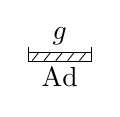
\begin{tikzpicture}[x=1mm, y=1mm, baseline=(alg.base)]
\node[inner sep=0pt] (alg) at (0,0) {$\mathfrak g$};
\draw[line width=.4pt] (-4,-1.3)--(-4,-3.2)--(4,-3.2)--(4,-1.3);
\draw[line width=.4pt] (-4,-2)--(4,-2);
\draw[line width=.3pt] (-3.5,-3.1)--(-2.7,-2.1) (-2,-3.1)--(-1.2,-2.1) (-.5,-3.1)--(.3,-2.1) (1,-3.1)--(1.8,-2.1) (2.5,-3.1)--(3.3,-2.1);
\node[anchor=north, inner sep=1pt] at (0,-3.5) {$\mathrm{Ad}$};
\end{tikzpicture}
and in $\mathfrak g^*$; there is a system of orbits there.
}}
\end{GelfandAdjacentEvidence}

All this is in a small nbhd of $e$ --- where there is \underline{\underline{$\exp$}}.



$\beta$ is constructed from the struct. const. of the algebra.



\begin{GelfandAdjacentEvidence}{GELFAND-P000208}{3}
[Crossed out: illegible.]
\Incomplete{GELFAND-P000208}{cancelled-word}{One word beneath dense repeated loops. Undetermined candidates: “Предложения” (Proposals) / “Продолжение” (Continuation). The letters beneath the strokes are illegible.}
\end{GelfandAdjacentEvidence}

\begin{center}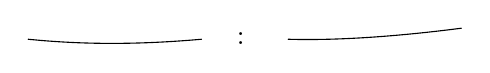
\begin{tikzpicture}[x=1mm, y=1mm]
\draw[line cap=round] (0,0).. controls (7,-.7) and (14,-.7)..(22,0);
\node[inner sep=0pt] at (27,.1) {:};
\draw[line cap=round] (33,0).. controls (40,-.2) and (48,.5)..(55,1.4);
\end{tikzpicture}\end{center}



\underline{Planned.}



1.\quad\uwave{Expository talks on logic.}\quad (including the solution of the continuum hypothesis)



2.\quad Lidskii “Asymptotics of eigenv. of self-adj. oper.”



3.\quad Work of Kirillov; Kazhdan; Graev.



\begin{center}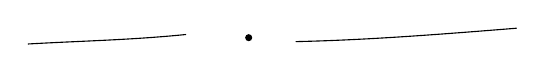
\begin{tikzpicture}[x=1mm, y=1mm]
\draw[line cap=round] (0,0).. controls (7,.4) and (13,.5)..(20,1.2);
\fill (28,.8) circle (.45mm);
\draw[line cap=round] (34,.3).. controls (43,.5) and (52,1.2)..(62,2);
\end{tikzpicture}\end{center}



\underline{Example.}\quad$G=SO (3)$,\quad$\mathfrak g=\mathbb R^3$,\quad$\mathfrak g^*=\mathbb R^3$,
\par the action --- rotations.
\par Orbit --- $S^2$.



\begin{GelfandAdjacentEvidence}{GELFAND-P000208}{4}
\begin{equation*}p (x)=\frac{\sin\tau}{\tau},\qquad\text{where }\tau=\lVert x\rVert.\end{equation*}
\Unclear{GELFAND-P000208}{radial-density}{The repeated radial-variable glyph has an upper stroke and a hooked leg: $\tau$ / $r$. Candidate in the line: $\tau$; the literal letter is undetermined. No square on the ratio is distinguishable.}
\end{GelfandAdjacentEvidence}

A fact from analysis\quad (on the Fourier transform of $\delta$ on $S_\lambda$)



\begin{GelfandAdjacentEvidence}{GELFAND-P000208}{5}
\begin{equation*}\left (\delta_{S_\lambda}\right)^{\vee}\equiv\frac{\sin\lambda\tau}{\tau}\end{equation*}
\Unclear{GELFAND-P000208}{fourier-sphere}{Above the closing parenthesis is a short two-stroke mark: $\sim$ / $\vee$. The densely inked sign between parenthesis and ratio: $\equiv$ / $=$. Candidates in the line: $\vee$, $\equiv$; neither reading is established. The radial variable is the same as in the preceding ratio: $\tau$ / $r$.}
\end{GelfandAdjacentEvidence}



\SourcePage{GELFAND-P000209}{unlabelled}
$\beta$ --- ordinary surface of the sphere.



\begin{GelfandAdjacentEvidence}{GELFAND-P000209}{1}
\underline{Answer.}
\begin{equation*}\chi (x)=\frac{\sin\lambda\tau}{\sin\tau}.\end{equation*}
\Unclear{GELFAND-P000209}{radial-character}{The radial grapheme is the same as on the preceding page: $\tau$ / $r$. Candidate in the ratio: $\tau$; the literal letter is undetermined.}
\end{GelfandAdjacentEvidence}

All this for $\lambda=2n+1$ (countably many repres.)



$\beta (x)$ --- $\int$ over cycles of the orbit of certain integral forms.



\uwave{Work of Fuchs and Gelfand.}



\underline{\underline{Fuchs.}} Study of principal bundles



\begin{GelfandAdjacentEvidence}{GELFAND-P000209}{2}
[Crossed out: illegible.]
\Incomplete{GELFAND-P000209}{cancelled-before-fiber}{A short, densely crossed-out entry between “bundles” and “with fiber”. The letters are undetermined.}
\end{GelfandAdjacentEvidence}

with fiber $G$ (top. group)



Types of invar. --- as top. spaces and classif. spaces.



\begin{GelfandAdjacentEvidence}{GELFAND-P000209}{3}
$\mathfrak g$ --- a group
\Unclear{GELFAND-P000209}{group-letter}{The looped group sign: lowercase fraktur-like $\mathfrak g$ / handwritten uppercase $G$. Candidate $\mathfrak g$ is repeated in subscripts, arrow labels, and under the hat; the upright $G$ above has a different form. The letter case is undetermined.}
\end{GelfandAdjacentEvidence}
\begin{GelfandAdjacentEvidence}{GELFAND-P000209}{4}




\SourceFigure{GELFAND-P000209}{universal-bundle}{\par\smallskip\centering{\color{black}\(\displaystyle 
\begin{tikzcd}[ampersand replacement=\&]E_{\mathfrak g}\arrow[d,"\mathfrak g"]\\B_{\mathfrak g}\end{tikzcd}
\qquad\text{--- universal bundle}
\)}}
\end{GelfandAdjacentEvidence}
\begin{GelfandAdjacentEvidence}{GELFAND-P000209}{5}

($E_{\mathfrak g}$ [Crossed out: illegible.]
\Incomplete{GELFAND-P000209}{cancelled-before-aspherical}{One word beneath repeated dense strokes before “aspherical”. The letters are undetermined.}
\end{GelfandAdjacentEvidence}

aspherical, i.e. $\pi_k (E_{\mathfrak g})=0$, $k>0$).



A char. class is determ. by specifying $\alpha\in H^q (B_{\mathfrak g}; A)$



\begin{GelfandAdjacentEvidence}{GELFAND-P000209}{6}
(Maps of principal bundles [перестан. / перестав. (commute?)] with the group action).
\Unclear{GELFAND-P000209}{equivariance-word}{The penultimate strokes before the period in the abbreviation “перестан.” / “перестав.” (commute?) are merged. Neither reading is established.}
\end{GelfandAdjacentEvidence}

Analogously, instead of $H^q$ --- any contravar. functor $h$ to the category of sets.



All char. classes --- $h (B_{\mathfrak g})$



(this is if $h$ --- a homotopy functor)



$\hat{\mathfrak g}$ --- a max. comp. subgroup



(all of them are $\underset{\text{and equiv. to }\mathfrak g.}{\text{homot. equiv.}}$ and their classif. spaces hom. equivalent.)



\begin{GelfandAdjacentEvidence}{GELFAND-P000209}{7}
G. \underline{Problem:} find the actual classif. space of noncomp. groups,
without identifying it with the max. comp. subgr.






\SourceFigure{GELFAND-P000209}{Hausdorff-bundle}{\par\smallskip\centering{\color{black}\(\displaystyle 
\begin{tikzcd}[ampersand replacement=\&]E\arrow[d,"\mathfrak g"]\\X\end{tikzcd}
\qquad\begin{aligned}
&\text{base \uwave{only Hausdorff}}\\
&\text{a condition replacing loc. triviality,}\\
&\text{which in the completely regul. case coincides}\\
&\text{with usu}\underline{\text{al}}\text{ loc. triv.}
\end{aligned}
\)}}
\end{GelfandAdjacentEvidence}



\SourcePage{GELFAND-P000210}{2}
\begin{flushright}$2$\end{flushright}



The following property is required to hold:



\begin{GelfandAdjacentEvidence}{GELFAND-P000210}{1}
\uwave{consider the cone over $\mathfrak g$}
\Unclear{GELFAND-P000210}{cone-heading}{The looped group sign is the same as on the preceding page: fraktur-like lowercase $\mathfrak g$ / handwritten uppercase $G$. Candidate in the lines and diagrams: $\mathfrak g$; the letter case is undetermined. The heading has a wavy underline.}
\end{GelfandAdjacentEvidence}
\begin{GelfandAdjacentEvidence}{GELFAND-P000210}{2}





\Unclear{GELFAND-P000210}{cone-sketch}{The outer cone outline, rounded base, and internal curved paths. Closure of the paths and possible arrow directions are undetermined.\par\smallskip\centering{\color{black}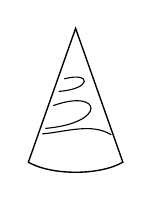
\begin{tikzpicture}[x=1mm, y=1mm, line cap=round]
\draw[line width=.5pt] (-6,0)--(0,17)--(6,0);
\draw[line width=.5pt] (-6,0)..controls(-3,-1.7)and(3,-1.7)..(6,0);
\draw[line width=.4pt] (-1.4,10.6)..controls(2,11.5)and(2.1,9.3)..(-2.1,9.0);
\draw[line width=.4pt] (-2.8,7.2)..controls(3.3,9.4)and(4.1,5.0)..(-3.8,4.3);
\draw[line width=.4pt] (-4.2,3.6)..controls(-1,3.9)and(2,5.0)..(4.5,3.5);
\end{tikzpicture}}}
\end{GelfandAdjacentEvidence}

$\mathfrak g$ acts on it with one fixed point.



$\forall x\in X$, $\exists$ a map $E\longrightarrow C\mathfrak g$, commuting



\begin{GelfandAdjacentEvidence}{GELFAND-P000210}{3}
with the group action; the fiber over [Crossed out: an illegible sign.]
\Incomplete{GELFAND-P000210}{cancelled-point}{Before $x$ a sign with a lower loop is densely crossed out. Undetermined candidates: $y$ / $g$.}
\end{GelfandAdjacentEvidence}

$x$ maps isomorphically onto the base of the cone



(Local triviality follows from this).



(For a completely regul. base (there exists a function $1$ at the point, $0$ outside a given nbhd)



loc. triviality $\Longrightarrow$ this property.)



(but in this case the theory becomes trivial and all computed invar. are trivial)



\begin{center}\begin{tikzpicture}[x=1mm, y=1mm]
\draw[line cap=round] (0,0)..controls(4,-.3)and(8,-.1)..(12,.1);
\fill (18,.3) circle(.22mm);
\draw[line cap=round] (24,.6)..controls(28,.9)and(33,.8)..(37,.9);
\end{tikzpicture}\end{center}



\uwave{D. Kazhdan's remark}: then the height of the cone determines a cont. function on $X$.



So this def. is incorrect.



\begin{center}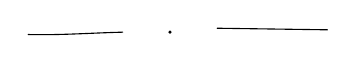
\begin{tikzpicture}[x=1mm, y=1mm]
\draw[line cap=round] (0,0)..controls(4,-.1)and(8,.2)..(12,.3);
\fill (18,.3) circle(.22mm);
\draw[line cap=round] (24,.8)--(38,.6);
\end{tikzpicture}\end{center}



\begin{GelfandAdjacentEvidence}{GELFAND-P000210}{4}
$\mathfrak g$ --- a Lie group,\quad$\mathfrak g\subset gL (n,\mathbb R)$ --- a closed subgr.
\Unclear{GELFAND-P000210}{linear-group-case}{The first letter before $L$ has a lower loop: $gL (n,\mathbb R)$ / $GL (n,\mathbb R)$. Candidate in the line: $gL$; the letter case is undetermined. The group sign itself is the same as in the cone heading.}
\end{GelfandAdjacentEvidence}

(i.e. $\mathfrak g$ acts on $\mathbb R^n$).



There exists a construction which makes a vector bundle (induced) from a principal bundle



$E^*=E\times\mathbb R^n/\mathfrak g$.



\begin{GelfandAdjacentEvidence}{GELFAND-P000210}{5}
$(x, y)=(gx, gy)$
\Unclear{GELFAND-P000210}{quotient-relation}{Between the pairs are two short dense strokes merged with the opening parenthesis of the right-hand pair: $=$ / $\sim$. Candidate in the line: $=$; the sign is undetermined.}
\end{GelfandAdjacentEvidence}
\begin{GelfandAdjacentEvidence}{GELFAND-P000210}{6}




\SourceFigure{GELFAND-P000210}{vector-bundle-diagram}{\par\smallskip\centering{\color{black}\(\displaystyle \begin{tikzcd}[ampersand replacement=\&]E^*\arrow[r]\arrow[d,"{\mathbb R^n}"]\&\mathbb R^n\\X\&\end{tikzcd}\)}}
\end{GelfandAdjacentEvidence}

There must exist a map $E^*\longrightarrow\mathbb R^n$,



\begin{GelfandAdjacentEvidence}{GELFAND-P000210}{7}
[Crossed out: illegible.]
\Incomplete{GELFAND-P000210}{cancelled-linear}{A short word before “linear” is crossed out by two strokes. The letters are undetermined.}
\end{GelfandAdjacentEvidence}

linear on the fibers and



such that at a certain point $x_0$\quad$\underset{\text{(given)}}{\phantom{x_0}}$



it --- an isomorphism.



(No compatibility with the group action).




\begin{tikzpicture}[x=1mm, y=1mm]
\draw[line cap=round] (0,25)..controls(-5,17)and(-5,7)..(0,0);
\fill (0,0) circle(.3mm);
\end{tikzpicture}



this is the def. of loc. triviality (for Hausd.) and this is precisely the requirement.



Kazhdan's remark cannot be repeated.





\SourcePage{GELFAND-P000211}{unlabelled}
$E$ is recovered from $E^*$.



One cannot construct a classif. space, but there is an analogue.



\underline{Example}:



\begin{GelfandAdjacentEvidence}{GELFAND-P000211}{1}
[An undetermined thickened sign.]
\Unclear{GELFAND-P000211}{before-group}{Before the group notation is a separate thickened sign with a lower loop and a transverse stroke: “в” (in) / a crossed-out earlier sign. Neither candidate is established.}
\end{GelfandAdjacentEvidence}
\begin{GelfandAdjacentEvidence}{GELFAND-P000211}{2}

$\mathfrak g=\mathbb R\subset gL (1,\mathbb R)$ --- matrices with $\det>0$.
\Unclear{GELFAND-P000211}{linear-group-case}{The first letter before $L$ has a lower loop: $gL$ / $GL$. Candidate in the line: $gL$; the letter case is undetermined. The looped group sign itself is the same as on the preceding pages: $\mathfrak g$ / $G$, candidate $\mathfrak g$.}
\end{GelfandAdjacentEvidence}

\uwave{A nontrivial} $\underset{\text{(principal)}}{\mathbb R\text{-bundle}}$ (also “universal”).



The direct product of countably many lines in the Tych. topology.



\begin{equation*}(x_1, x_2,\ldots)\quad\text{--- sequences}\end{equation*}



\begin{equation*}\alpha (x_1,\ldots)=(x_1e^\alpha,\ldots)\end{equation*}



The quotient space $S$ cannot be embedded in $E$ (!) ---
--- there are no sections.



\underline{Fact:} in $\mathbb R^\infty$ one cannot choose one point on each ray.



\Needspace{6\baselineskip}\underline{Proof.}



$S$ is Hausdorff, but every cont. function on it is $\mathrm{const}$,



so such a map --- to a point (coords. --- cont. functions).



\begin{GelfandAdjacentEvidence}{GELFAND-P000211}{3}
(Show that with [рассет. / рассеч.? (section?)]
\Unclear{GELFAND-P000211}{section-word}{After “with” the source abbreviation is “рассет.” / “рассеч.” (section?). The last letter has an upper stroke and a downward stroke; the reading is undetermined.}
\end{GelfandAdjacentEvidence}

\begin{equation*}\sum\frac{1}{2^n}\frac{|x_i|}{1+|x_i|}=1/2\end{equation*}



one obtains a discontinuous map.)



Suppose there is $f$. (a cont. function).



\begin{equation*}(x_1, x_2,\ldots)\end{equation*}



\begin{equation*}a_i=f (\underbrace{0,\ldots,0}_{i},1,\ldots,1,\ldots)\end{equation*}



\begin{equation*}a=f (x_1, x_2,\ldots)\end{equation*}



We shall prove that $a=\lim_{i\to\infty}a_i$.



$\forall\varepsilon>0$ $\exists$ a nbhd of the point



\begin{GelfandAdjacentEvidence}{GELFAND-P000211}{4}
[Crossed out: an illegible sign.]
\Incomplete{GELFAND-P000211}{cancelled-point}{Before the coordinate parenthesis a sign is densely crossed out. The original grapheme is undetermined.}
\end{GelfandAdjacentEvidence}

$(x_1, x_2,\ldots)\in S$,



where the difference is $<\varepsilon$. (from $a$).



\begin{equation*}(x_1^0, x_2^0,\ldots)\end{equation*}



(A neighborhood --- if the preimage is open)





\SourcePage{GELFAND-P000212}{3}
\begin{flushright}$3$\end{flushright}



A neighborhood in $E$



\begin{equation*}\begin{gathered}|x_1-x_1^0|<\delta\\\cdots\\|x_N-x_N^0|<\delta.\end{gathered}\end{equation*}



Make these coords. the same, the others very large.



\begin{equation*}\left (\frac{x_1^0}{M},\ldots,\frac{x_N^0}{M},1,1,\ldots\right),\end{equation*}



and by these the point $(0,\ldots,0,1,\ldots,1,\ldots)$ is approxim.



\begin{GelfandAdjacentEvidence}{GELFAND-P000212}{1}
A map always exists (but is not unique)






\Unclear{GELFAND-P000212}{bundle-square}{The upper-left vertex is rounded: calligraphic $\mathcal E$ / $\varepsilon$. Candidate in the diagram: $\mathcal E$; the letter is undetermined. Both horizontal arrows point right, both vertical arrows down with labels $\mathbb R$.\par\smallskip\centering{\color{black}\(\displaystyle \begin{tikzcd}[ampersand replacement=\&]\mathcal E\arrow[r]\arrow[d,"\mathbb R"]\&E\arrow[d,"\mathbb R"]\\X\arrow[r]\&S\end{tikzcd}\)}}
\end{GelfandAdjacentEvidence}

$S$ is constructed from a product of $\mathbb R$ of any cardinality (depends on $X$)



$25/\overline{\underline{\mathrm{IX}}}$.



\underline{\underline{A good formula}} (Feynman)



\begin{equation*}\frac{1}{ab}=\int_0^1\frac{dt}{(at+b (1-t))^2}\end{equation*}



(decomp. into partial fractions)



\begin{equation*}\frac{1}{abc}=\int_\Delta\frac{dt_1\, dt_2}{(at_1+bt_2+ct_3)^3},\end{equation*}



$\Delta$ --- a simplex
\begin{equation*}t_1+t_2+t_3=1,\quad t_i\geq0.\end{equation*}



Next time \uwave{Fuchs} and then \uwave{logic}.



There is a counterexample to the hypothesis of a common fixed point of commuting cont. maps of an interval, and it is proved
that if they are differentiable, there is a point fixed for one and of finite multiplicity for the other.





\SourcePage{GELFAND-P000213}{unlabelled}
\underline{Fuchs} (continuation).



\begin{GelfandAdjacentEvidence}{GELFAND-P000213}{1}
$\mathfrak g\subset gL (n;\mathbb R)$
\Unclear{GELFAND-P000213}{linear-group-case}{The first letter before $L$ has a lower loop: $gL$ / $GL$; a semicolon follows $n$. Candidate in the line: $gL$. The group sign itself is the same as before: $\mathfrak g$ / $G$, candidate $\mathfrak g$; the letter case is undetermined.}
\end{GelfandAdjacentEvidence}

principal bundles



\begin{equation*}\begin{aligned}(\xi)&\qquad p: E\longrightarrow X\\(\xi^{\#})&\qquad p^{\#}: E^{\#}\longrightarrow X\end{aligned}\end{equation*}



($X$ --- Hausdorff)



\begin{GelfandAdjacentEvidence}{GELFAND-P000213}{2}
($\mathfrak g$ acts on $E$ without fixed points]
\Unclear{GELFAND-P000213}{action-free}{The right-hand entry about an action without fixed points. The closing sign is angular: $]$ / $)$. Candidate in the line: $]$; the reading is undetermined.}
\end{GelfandAdjacentEvidence}

\begin{tikzpicture}[x=1mm, y=1mm]\draw[line cap=round] (0,4)..controls(-.3,2)and(.3,1)..(1,0);\end{tikzpicture}
\begin{equation*}\begin{gathered}xg_1=xg_2\Rightarrow\\\Rightarrow g_1=g_2\end{gathered}\end{equation*}



Loc. triviality: $\forall x$ $\exists$ a map $E^{\#}\longrightarrow\mathbb R^n$,
an isom. at the point $x$, linear on the fibers.



\begin{GelfandAdjacentEvidence}{GELFAND-P000213}{3}
(One cannot require $0$ outside small nbhds, since then even $X\times\mathbb R^n$ may
fail to qualify because of nonregularity)





\SourceFigure{GELFAND-P000213}{morphism}{\par\smallskip\centering{\color{black}A morphism --- a map
\begin{equation*}\begin{tikzcd}[ampersand replacement=\&]E_1\arrow[r]\arrow[d]\&E_2\arrow[d]\\X_1\arrow[r]\&X_2\end{tikzcd}\end{equation*}
, commuting with the action of $\mathfrak g$.
}}
\end{GelfandAdjacentEvidence}

\dashuline{Examples of functors}:



1) cohomology



2) $H$-bundles ($H$ --- another group)



correspondingly charact. classes.



$h_{\mathrm{alg}}(\mathfrak g)$ --- the set (group) of all char. classes constructed from the functor $h$.



1) For any top. space



\begin{GelfandAdjacentEvidence}{GELFAND-P000213}{4}
[Crossed out: an illegible sign.]
\Incomplete{GELFAND-P000213}{corrected-topological}{After “пр-ва” (space), before $X$, an additional sign is densely crossed out. The original grapheme is undetermined.}
\end{GelfandAdjacentEvidence}

$X$, the sheaf $\mathbb R$ of germs of cont. real functions on $X$ is defined.



Put



\begin{equation*}h (X)=H^q (X,\mathbb R).\end{equation*}



\begin{GelfandAdjacentEvidence}{GELFAND-P000213}{5}
(for [Crossed out: illegible.]
\Incomplete{GELFAND-P000213}{cancelled-paracompact}{A fragment between “for” and “paracomp.” is crossed out; a descender is visible. The letters are undetermined.}
\end{GelfandAdjacentEvidence}

paracomp. $X$ this is $0$)



\begin{GelfandAdjacentEvidence}{GELFAND-P000213}{6}
There is defined



\begin{equation*}H_{\mathrm{alg}}^q (\mathfrak g)\end{equation*}



\underline{\underline{Answer.}} For semisimple $\mathfrak g$ having finitely many connected components



\begin{equation*}H_{\mathrm{alg}}^q (\mathfrak g)=\underline{H^q (\bar{\mathfrak g}/\hat{\mathfrak g}; R)}\end{equation*}
\Unclear{GELFAND-P000213}{final-quotient}{Above the first right-hand group sign is a straight bar, above the second an angular hat; a slash separates them. Candidate in the line: $\bar{\mathfrak g}/\hat{\mathfrak g}$. A descender from the preceding line overlaps the upper strokes; the reading of the first superscript mark remains open. The whole right-hand side is underlined.}
\end{GelfandAdjacentEvidence}

\begin{flushright}\begin{minipage}{.55\linewidth}
with coeffs. in a constant sheaf ---\\--- real coeffs.
\end{minipage}\end{flushright}





\SourcePage{GELFAND-P000214}{4}
\begin{flushright}$4$\end{flushright}



Here $\bar{\mathfrak g}$ --- a compact form of $\mathfrak g$



$\hat{\mathfrak g}$ --- a max. comp. subgroup



\begin{GelfandAdjacentEvidence}{GELFAND-P000214}{1}
[Crossed out: $\bar{\mathfrak g}$?]
\Incomplete{GELFAND-P000214}{cancelled-subgroup}{Before the final group sign an entry is densely crossed out. Candidate $\bar{\mathfrak g}$ from the visible upper bar and lower loop; the precise form beneath the strokes is undetermined.}
\end{GelfandAdjacentEvidence}
\begin{GelfandAdjacentEvidence}{GELFAND-P000214}{2}

$\mathfrak g$.
(For $\mathfrak g=gL (n, R)$
\Unclear{GELFAND-P000214}{linear-group-case}{The initial letter before $L$ matches the looped lowercase group sign: $gL$ / $GL$. Candidate in the line: $gL$; the letter case is undetermined. The group sign itself is the same as before: $\mathfrak g$ / $G$, candidate $\mathfrak g$.}
\end{GelfandAdjacentEvidence}

there will be $\bar{\mathfrak g}=U (n)$, $\hat{\mathfrak g}=O (n)$



$\bar{\mathfrak g}$ is obtained as a max. comp. subgroup of the complexification of $\mathfrak g$)



\underline{2nd order}: as for $S^2$.



For a compact group everything is trivial.



For a nonsemisimple one, take $\mathfrak g/\hat{\mathfrak g}$ and differ. forms on $\mathfrak g/\hat{\mathfrak g}$ invariant under $\mathfrak g$.



$d (\text{invar.})$ --- invar. And the homologies of this complex are isomorphic to $H_{\mathrm{alg}}^q (\mathfrak g)$.



\begin{samepage}
\begin{equation*}H_{\mathrm{alg}}^q (\mathbb R;\mathbb R)=\begin{cases}R&q=0,1\\0&q>1.\end{cases}\end{equation*}



Check! (there are $1$ and $dx$)
\end{samepage}



2) $X$, $H$ --- a top. group



$EH (X)$ --- the set of all loc. triv. (in the usual sense) bundles (principal) on $X$.



\begin{tikzpicture}[x=1mm, y=1mm]\draw[line width=.3pt] (0,5)--(1,0);\end{tikzpicture}



\underline{Theorem.}



\begin{equation*}EH_{\mathrm{alg}}(\mathfrak g)=\operatorname{Hom}(\mathfrak g, H)\end{equation*}



\begin{GelfandAdjacentEvidence}{GELFAND-P000214}{3}
(cont. hom. [Crossed out: an illegible sign.]
\Incomplete{GELFAND-P000214}{cancelled-parenthesis}{After “cont. hom.” are doubled curved and oblique strokes: a cancelled $)$ / the sign $\varphi$. The reading is undetermined.}
\end{GelfandAdjacentEvidence}

, more precisely, classes of conjugate homom.)



The natural answer --- a hom. $\mathfrak g\longrightarrow H$ corresponds to a char. class, naturally defined.



\begin{GelfandAdjacentEvidence}{GELFAND-P000214}{4}
\begin{equation*}\varphi_1\sim\varphi_2,\ \text{if}\ \exists h\in H,\qquad\varphi_1(g)=h^{-1}\varphi_2(g)h\end{equation*}
\Unclear{GELFAND-P000214}{conjugacy}{The map signs have diverging upper strokes and a long stem: $\varphi$ / $\psi$. Candidate in the line: $\varphi$, in both indexed names. The exact Greek letter is undetermined. The sign $\sim$, $h^{-1}$, and order of factors are readable.}
\end{GelfandAdjacentEvidence}



\begin{GelfandAdjacentEvidence}{GELFAND-P000215}{1}
\SourcePage{GELFAND-P000215}{unlabelled}
\uwave{Construction of a universal bundle.}







\Unclear{GELFAND-P000215}{universal-inclusions}{At the top is an elongated inclusion with a rightward arrowhead on the upper stroke. The precise reading as $\hookrightarrow$ / $\subset$ with an added arrow is undetermined. There is a downward arrow on the left and $\subset$ below; there is no right vertical arrow. The rounded upper letter is rendered by candidate $\mathcal E$.\par\smallskip\centering{\color{black}\begin{tikzpicture}[x=1mm, y=1mm]
\node (EI) at (0,0) {$\mathcal E_{\mathfrak g}^I$};
\node (EJ) at (42,0) {$\mathcal E_{\mathfrak g}^J$};
\node (SI) at (0,-18) {$S_{\mathfrak g}^I$};
\node (SJ) at (42,-18) {$S_{\mathfrak g}^J$};
\draw[->] (EI.south)--(SI.north);
\draw[->,line width=.5pt] (14,2)--(28,2);
\draw[line width=.4pt] (14,1)..controls(12,1)and(12,-1.5)..(15,-1.5)--(27,-1.5);
\node at (21,-18) {$\subset$};
\end{tikzpicture}}}
\end{GelfandAdjacentEvidence}

$I\subset J$ --- arbitrary sets.



Any bundle maps into a universal one with $I$ of sufficiently large cardinality.



Consider $\mathbb R^I\ni (x_i,\ i\in I)$.



The topology --- Tychonoff.



and $\underset{\scriptstyle n\text{ lin. indep. vect.}}{n\text{-frames}}$ in it --- this is precisely $\mathcal E_{\mathfrak g}^I$.



\begin{GelfandAdjacentEvidence}{GELFAND-P000215}{2}
$gL (n,\mathbb R)$ and $\mathfrak g$ act there.
\Unclear{GELFAND-P000215}{linear-group-case}{The initial letter before $L$ matches the lower looped group sign on the right: $gL$ / $GL$. Candidate in the line: $gL$; the letter case is undetermined. The group sign itself is rendered by the same candidate $\mathfrak g$ as before.}
\end{GelfandAdjacentEvidence}

The quotient space is precisely our $S_{\mathfrak g}^I$.



Observe that $\mathcal E_{\mathfrak g}^I$ does not depend on $\mathfrak g$.



\underline{Lemma.} $\forall\mathcal E_{\mathfrak g}^I$ and a cont. function $f$ on it $\exists$



$J\subset I$ such that $I\setminus J$ is at most countable, and



and $\left.f\right|_{\mathcal E_{\mathfrak g}^J}=\mathrm{const}$.





\SourcePage{GELFAND-P000216}{6}
\begin{flushright}$6$\end{flushright}



$2/\overline{\underline{\mathrm X}}$.\quad\underline{\underline{Fuchs.}}



$T$ --- a space, $S\subset\operatorname{Map}(T, T)$, compact open top.



\begin{GelfandAdjacentEvidence}{GELFAND-P000216}{1}
$\mathfrak g$ acts on $T$ on the right
\Unclear{GELFAND-P000216}{group-letter}{The group sign is looped: lowercase fraktur-like $\mathfrak g$ / handwritten uppercase $G$. Candidate in the lines, subscripts, and diagrams: $\mathfrak g$. The element sign $g$ in the next line is simpler; the letter case of the group sign is undetermined.}
\end{GelfandAdjacentEvidence}

\begin{equation*}f\in S,\quad g\in\mathfrak g\Rightarrow fg\in S,\ gf\in S.\end{equation*}



\underline{Examples.}



\begin{GelfandAdjacentEvidence}{GELFAND-P000216}{2}
$1^{\circ}$. $\mathfrak g\subset gL (n; R)$,
\Unclear{GELFAND-P000216}{linear-group-case}{In the first example $gL (n; R)$ / $GL (n; R)$; the initial letter is looped. Candidate in the line: $gL$; the letter case is undetermined.}
\end{GelfandAdjacentEvidence}

$T=\mathbb R^n$; $S$ --- all lin. maps (including zero maps).



\begin{GelfandAdjacentEvidence}{GELFAND-P000216}{3}
$2^{\circ}$. $\mathfrak g$ --- a Hausdorff top. group, $T=C\mathfrak g$ --- the cone over $\mathfrak g$







\SourceFigure{GELFAND-P000216}{cone-diagram}{\par\smallskip\centering{\color{black}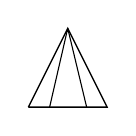
\begin{tikzpicture}[x=1mm, y=1mm]
\draw[line width=.5pt] (0,0)--(5,10)--(10,0)--(0,0);
\draw[line width=.4pt] (5,10)--(2.7,0) (5,10)--(7.4,0);
\end{tikzpicture}}}
\end{GelfandAdjacentEvidence}

$\mathfrak g$ acts naturally, $S$ is generated by them and similarities



\begin{GelfandAdjacentEvidence}{GELFAND-P000216}{4}
[Crossed out: растя... / растяже...? (dila...?)]
\Incomplete{GELFAND-P000216}{cancelled-dilation}{Before “contractions” a word or beginning of a word is crossed out; the opening “раст...” is distinguishable. The ending is undetermined.}
\end{GelfandAdjacentEvidence}

contractions toward the vertex (and to a point).



\underline{Axioms.}



$1^{\circ}$. $T$ is contractible by transformations in $S$ to a marked point $\ast$.



$2^{\circ}$. $\mathfrak g$ is closed in the group of all homeom. of $T$ to itself.



$3^{\circ}$. $\ast$ is fixed under all transf. in $S$.



$4^{\circ}$. $\varphi_t: T\longrightarrow T$



\begin{GelfandAdjacentEvidence}{GELFAND-P000216}{5}
\begin{equation*}\begin{gathered}\varphi_0=\text{identity},\quad\varphi_t\in S\quad\text{---}\\\varphi_1(T)=\ast\end{gathered}\end{equation*}
\Unclear{GELFAND-P000216}{axiom-four-homotopy}{The Greek map sign has diverging upper strokes and a stem: $\varphi$ / $\psi$. Candidate in the fourth axiom and following phrase: $\varphi$; the exact letter is undetermined. Subscripts $0$, $t$, $1$, identity, and image $\ast$ are readable.}
\end{GelfandAdjacentEvidence}

--- the homotopy of axiom $1^{\circ}$.



Then there exist $\varphi_t$ such that $\varphi_t$ for $t<1$ are topological embeddings.



$5^{\circ}$. $S$ contains all transf. of $\mathfrak g$, and maps
close to maps of $\mathfrak g$ in $S$ are top. embeddings.



$U (1)\subset S$ consists of embeddings.



\begin{GelfandAdjacentEvidence}{GELFAND-P000216}{6}
In this situation spaces are defined






\SourceFigure{GELFAND-P000216}{universal-map}{\par\smallskip\centering{\color{black}\(\displaystyle \begin{tikzcd}[ampersand replacement=\&]\mathcal E_{\mathfrak g}\arrow[d]\\S_{\mathfrak g}\end{tikzcd}\)


, the action of $\mathfrak g$ on $\mathcal E_{\mathfrak g}$ --- a universal principal bundle.
}}
\end{GelfandAdjacentEvidence}





\begin{equation*}\underbrace{T\times\cdots\times T}_{I\text{ times}}\qquad\text{Tych. topology.}\end{equation*}



\begin{GelfandAdjacentEvidence}{GELFAND-P000216}{7}
$6^{\circ}$. $\mathfrak g$ acts effectively on $T$,



(otherwise [удвл. / удовл.?] point)
\Unclear{GELFAND-P000216}{final-abbreviation}{The final parenthesis contains the abbreviation “удвл.” / “удовл.”. The reading and expansion of the word are undetermined.}
\end{GelfandAdjacentEvidence}



\begin{GelfandAdjacentEvidence}{GELFAND-P000217}{1}
\SourcePage{GELFAND-P000217}{unlabelled}
An element of $\mathcal E_{\mathfrak g}$ --- any embedding $T\subset T^I$ such
that its compositions with all projections lies in $S$.
\Unclear{GELFAND-P000217}{group-letter}{In the subscript of the rounded E and subsequently in $C\mathfrak g$, the action, and cohomology, the group sign is looped: $\mathfrak g$ / handwritten uppercase $G$. Candidate: $\mathfrak g$; the letter case is undetermined.}
\end{GelfandAdjacentEvidence}

1) $T=\mathbb R^n$ --- all $n$-frames.



2) $T=C\mathfrak g$, $\mathcal E_{\mathfrak g}=C\mathfrak g\times\ldots\times C\mathfrak g\setminus\{\ast,\ldots,\ast\}$.



$\mathfrak g$ acts on $\mathcal E_{\mathfrak g}$ by multiplication by transf. in $\mathfrak g$.



\begin{GelfandAdjacentEvidence}{GELFAND-P000217}{2}
\begin{equation*}
I\text{ finite}\quad\Rightarrow\quad
\begin{aligned}
&1)\ \text{the usual classif. space}\\
&2)\ \text{Milnor's constr. with a not very substantial modification.}
\end{aligned}
\end{equation*}







\SourceFigure{GELFAND-P000217}{ray-example}{\par\smallskip\centering{\color{black}$\mathfrak g=\mathbb R$, $T={}$
\begin{tikzpicture}[baseline=-0.5ex]
\draw (0,0)--(1.6,0);
\fill (0,0) circle (1.5pt);
\end{tikzpicture}}}
\end{GelfandAdjacentEvidence}

$\mathcal E_{\mathfrak g}$ --- sequences of nonneg. numbers.



\begin{GelfandAdjacentEvidence}{GELFAND-P000217}{3}
For each $T$ its own definition of loc. triviality.







\SourceFigure{GELFAND-P000217}{principal-diagram}{\par\smallskip\centering{\color{black}\begin{tikzcd}[row sep=small, ampersand replacement=\&]
E \arrow[d,"\mathfrak g"]\\ X
\end{tikzcd}}}
\end{GelfandAdjacentEvidence}
\begin{GelfandAdjacentEvidence}{GELFAND-P000217}{4}

is loc. triv. if the induced bundle







\SourceFigure{GELFAND-P000217}{induced-diagram}{\par\smallskip\centering{\color{black}\begin{tikzcd}[row sep=small, ampersand replacement=\&]
E^{\#} \arrow[d,"T"]\\ X
\end{tikzcd}}}
, has the property:
$\forall x\ \exists$ a map $E^{\#}\longrightarrow T$, a homeom. on the fiber over $x$, and
on $\forall$ fiber it is a transf. in $S$.




\end{GelfandAdjacentEvidence}
\underline{Theorem.}



Every bundle maps into this one.



($X$ --- all Hausdorff)



Defined $H^q_{\mathrm{alg}}(\mathfrak g;\mathbb R)$



\underline{Theorem.}



Whatever $T$ and $S$ may be, $H^q_{\mathrm{alg}}(\mathfrak g,\mathbb R)$
does not depend on their choice



(Instead of $\mathbb R$ one may take a group $A$)



\underline{What will there be?}



Uspenskii, Lectures on logic 2



Lidskii, Asymptotics of eigenfns. (after Hörmander)



Sinai, Conditions on diffeom. under which there is an invar. measure



Kazhdan, Discr. groups --- solution of Selberg's problem



Kushnirenko, Analyt. action of a semisimple group in a nbhd. of a fixed point --- linear







\SourcePage{GELFAND-P000218}{7}
Tyurina and S. Gelfand\quad survey of Pham's works.

Anosov and Maslov

I. Bernstein\quad $P^{\lambda}$

Gelfand, Graev

\begin{GelfandAdjacentEvidence}{GELFAND-P000218}{1}
S. G. Krein\quad \Unclear{GELFAND-P000218}{list-interpolation}{Интерполяции / Интерполяция (interpolation); the ending is uncertain.}
\end{GelfandAdjacentEvidence}


$\begin{gathered}\text{Berezin}\\\text{Kirillov}\end{gathered}$,\quad Grassmann analysis.

\begin{center}
$\text{—}\,\bullet\,\text{—}$
\end{center}





\begin{GelfandAdjacentEvidence}{GELFAND-P000219}{1}
\SourcePage{GELFAND-P000219}{unlabelled}
$16/\underline{\overline{\mathrm{X}}}$\quad \Unclear{GELFAND-P000219}{heading-cancelled}{[Crossed out: illegible.]}
\end{GelfandAdjacentEvidence}
\quad \underline{S. G. Krein.}

\begin{GelfandAdjacentEvidence}{GELFAND-P000219}{2}
\underline{On interpolation of linear operators.}






\SourceFigure{GELFAND-P000219}{endpoint-map}{\par\smallskip\centering{\color{black}\(\displaystyle 
\left.
\begin{aligned}
 E_0,\ &\overset{A}{\longrightarrow}\ F_0,\\
 E_1,\ &\overset{A}{\longrightarrow}\ F_1,
\end{aligned}
\right\}\quad\text{Banach spaces,}
\)}}
\end{GelfandAdjacentEvidence}
\begin{GelfandAdjacentEvidence}{GELFAND-P000219}{3}

\Unclear{GELFAND-P000219}{upper-embedding}{all embedded / all are embedded}
\end{GelfandAdjacentEvidence}
 into one T. L. S. (the left and the right ones)

$A$ is bounded.

$E$, $F$ — an interpolation pair if, for $\forall\ A$, boundedness
at $0$ and $1$ implies boundedness of $A: E\longrightarrow F$.



All spaces will be spaces of summable functions.



\begin{GelfandAdjacentEvidence}{GELFAND-P000219}{4}
A Banach space of summable functions [Inserted below the line: on $[0,1]$.]
\Unclear{GELFAND-P000219}{definition-abbreviation}{на / наз. (on / called)}
\end{GelfandAdjacentEvidence}
 symmetric if

1) $y (t)\in E$
\begin{equation*}
 |x (t)|\leq |y (t)|\quad\Longrightarrow\quad x\in E
 \qquad\text{and}\qquad \|x\|\leq\|y\|
\end{equation*}



2) The norm does not change under transformations preserving measure
(one may consider an equimeasurable monotone one)



Then $L_\infty\subset E\subset L_1$.



\begin{GelfandAdjacentEvidence}{GELFAND-P000219}{5}
\underline{Examples.} 1)
\begin{equation*}
 \int_0^1 x^*(t)\, d\psi (t),\qquad \psi (t)\text{ — monot.}
 \qquad\text{— }\underline{\text{of Lorentz type}}
\end{equation*}
\Unclear{GELFAND-P000219}{lorentz-example}{In the differential, the monotonicity label, and the denominator of the next example, the Greek sign has three upper arms and a lower stroke: $\psi$ / $\Psi$. Candidate: $\psi$; the letter case is undetermined.}
\end{GelfandAdjacentEvidence}

$x^*(t)$ — a rearrangement of $|x (t)|$



2) Dual.\quad
$\displaystyle\sup_e\frac{\int_e|x (t)|\, dt}{\psi (me)}$



3) and Orlicz spaces (these include $L_p$)



[At the left above the line:] 1st step.

Riesz–Thorin theorem.





\SourcePage{GELFAND-P000220}{unlabelled}
2nd step.

Marcinkiewicz theorem.

(Less is required at the endpoints)



\begin{equation*}
 n_x (\tau)=\operatorname{mes}\{t:|x (t)|\geq\tau\}
\end{equation*}



\begin{equation*}
 [n_{Ax}(\tau)]^{1/q_i}\leq\frac{C}{\tau}\|x\|_{L_{p_i}}
\end{equation*}
— a less restrictive condition.



Most operators of analysis satisfy the Marcinkiewicz conditions at the endpoints



\underline{Matsaev and Dikarev} — more precisely, from $L_p$ into a space narrower than $L_q$
(of Lorentz type)! — and it is already minimal (in the middle)



(Minimal for \underline{all} operators
under conditions both of Marcinkiewicz and of Riesz–Thorin) —



— this is for improving operators:
\begin{equation*}
\begin{gathered}q_1>p_1\\q_2>p_2\end{gathered}
\quad\Big\Vert\quad\text{— as in the Marcinkiewicz theorem.}
\end{equation*}



$p=q$ — maps into itself — then all the other scales do too.



Let
$\begin{gathered}L_1\longrightarrow L_1\\L_\infty\longrightarrow L_\infty\end{gathered}$
\quad and $\|A\|\leq1$



\begin{GelfandAdjacentEvidence}{GELFAND-P000220}{1}
List all \Unclear{GELFAND-P000220}{middle-cancelled}{[Crossed out: illegible.]}
\end{GelfandAdjacentEvidence}
\begin{GelfandAdjacentEvidence}{GELFAND-P000220}{2}
 spaces for which $\|A\|\leq1$ as well.







\SourceFigure{GELFAND-P000220}{diagram-pair}{The purpose and direction of the additional oblique strokes are undetermined.\par\smallskip\centering{\color{black}
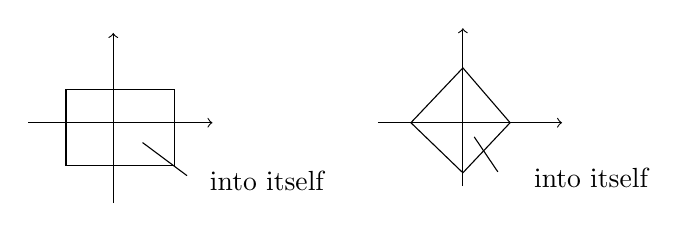
\begin{tikzpicture}[x=12mm, y=12mm, baseline=0pt]
\draw (-0.5,0.35)--(0.65,0.35)--(0.65,-0.45)--(-0.5,-0.45)--cycle;
\draw[->] (-0.9,0)--(1.05,0);
\draw[->] (0,-0.85)--(0,0.95);
\draw (0.31,-0.21)--(0.78,-0.56);
\node[anchor=west] at (0.92,-0.62) {into itself};
\begin{scope}[shift={(3.7,0)}]
\draw (-0.55,0)--(0,0.58)--(0.5,0)--(0,-0.53)--cycle;
\draw[->] (-0.9,0)--(1.05,0);
\draw[->] (0,-0.67)--(0,1);
\draw (0.12,-0.15)--(0.37,-0.52);
\node[anchor=west] at (0.65,-0.58) {into itself};
\end{scope}
\end{tikzpicture}
}}
\end{GelfandAdjacentEvidence}

[To the right of the figures:] linear oper. (2-dimensional case).

\begin{GelfandAdjacentEvidence}{GELFAND-P000220}{3}
Док. [prove / proved], that these are all symmetric norms and only they.
\Unclear{GELFAND-P000220}{linear-2d}{The abbreviation “Док.” is readable; the full verb form is not written. Possible expansions: prove / proved.}
\end{GelfandAdjacentEvidence}

General theorem — B. S. Mityagin.

It is necessary and sufficient that the space be symmetric.

(also in the $\infty$-dimensional case)



$L_p\overset{A}{\longrightarrow}L_p$\qquad what then?

$p\ne1,\infty$

(Marcinkiewicz case)



\begin{equation*}
 \bigl\Vert\underset{\substack{\vert\\\text{char. fn. }e}}{\chi_e}\bigr\Vert_E=\varphi (me).
\end{equation*}



(symmetry is again necessary)



the resulting function $\varphi (t)$ — a characteristic of the space $E$.



\begin{equation*}
 \ell_E=\underline{\lim}_{t\to0}\frac{\varphi (2t)}{\varphi (t)}
 \qquad
 u_E=\overline{\lim}_{t\to0}\frac{\varphi (2t)}{\varphi (t)}
 \qquad 1\leq\ell_E\leq u_E\leq2
\end{equation*}





\SourcePage{GELFAND-P000221}{9}
For $L_p$ they are both equal to $2^{1/p}$

Boundedness of all such $A$ in $E$ $\Longleftrightarrow$ $1<\ell_E\leq u_E<2$

(Semyonov's 1st theorem)



\begin{GelfandAdjacentEvidence}{GELFAND-P000221}{1}
Mityagin's theorem has not been generalized.
\begin{equation*}
 L_{1/\alpha}\longrightarrow L_{1/\alpha-\Delta}
\end{equation*}
\Unclear{GELFAND-P000221}{upper-target-exponent}{The right subscript is written as a diagonal fraction without parentheses: $1/\alpha-\Delta$ / $1/(\alpha-\Delta)$. The grouping is undetermined.}
\end{GelfandAdjacentEvidence}

$0<\Delta\leq\alpha_0<\alpha<\alpha_1$.



How can one list the spaces in which operators of this type are bounded?



\begin{equation*}
 2^{\alpha_0}<\ell_E\leq u_E<2^{\alpha_1}\quad\Longrightarrow\quad E\longrightarrow E_\Delta,
\end{equation*}



\begin{GelfandAdjacentEvidence}{GELFAND-P000221}{2}
where \Unclear{GELFAND-P000221}{after-where-cancelled}{After “where” there are two dense short signs; their exact reading and whether they are crossed out are undetermined.}
\end{GelfandAdjacentEvidence}

\begin{equation*}
 \|x\|_{E_\Delta}=\|x^*(t)t^{-\Delta}\|_E
\end{equation*}
(This generalizes the theorem of Dikarev and Matsaev — the best space)



\begin{GelfandAdjacentEvidence}{GELFAND-P000221}{3}
\underline{Applic.:}\quad Hausdorff–Young inequality
\begin{equation*}
 \sqrt[p]{|c_k|^p}\leq\|x\|_{L_p}\qquad\text{— from Riesz's theorem}
\end{equation*}
\Unclear{GELFAND-P000221}{hausdorff-formula}{The first radicand visibly contains $|c_k|^p$; no separate summation sign is distinguishable. The root index is $p$, and the right-hand norm is in $L_p$.}
\end{GelfandAdjacentEvidence}

Poia inequality:
\begin{equation*}
 \sqrt[p]{\sum k^{p-2}c_k^{*p}}\leq C\|x\|_{L_p}
\end{equation*}



$c_k^*$ — the monotone rearrangement of the $|\ |$ coefficients.



For monotone decreasing Fourier coefficients — two-sided inequalities (Hardy–Littlewood)



Between $L_1$ and $L_{1,5}$ there is no Hilbert interpolation space (Semyonov)



\underline{Gelfand's question:} an abstract description of interpolation spaces.
(it is unknown whether they are spaces of functions.)



\underline{Ya. Sinai.}

\begin{GelfandAdjacentEvidence}{GELFAND-P000221}{4}
\underline{Construction of invar. measures of smooth maps}\quad\underline{Markov partitions}





\SourceFigure{GELFAND-P000221}{torus-cell}{\par\smallskip\centering{\color{black}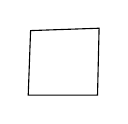
\begin{tikzpicture}
\draw (0,0)--(0.03,0.82)--(0.9,0.85)--(0.88,0)--cycle;
\end{tikzpicture}\par\smallskip
$T (x_1, x_2)=(ax_1+bx_2,\ cx_1+dx_2)$ — a map of the torus
}}
\end{GelfandAdjacentEvidence}

and $T_1$. — another.

\begin{GelfandAdjacentEvidence}{GELFAND-P000221}{5}
When does there exist a measurable map of the torus, $M\overset{U}{\longrightarrow}M$,
such that $UT_1=T_2U$.
\Unclear{GELFAND-P000221}{torus-map-indices}{First $T$, then $T_1$; in the equation, $T_1$ and $T_2$. The sign on the arrow and on both sides of the equation is looped: $U$ / $u$; candidate: $U$, with letter case undetermined.}
\end{GelfandAdjacentEvidence}

Irrational eigenvalues $\Rightarrow$ real $\Rightarrow$ ergodic, the spectrum
is Lebesgue of countable multiplicity.



Entropy $h (T)=\ln\lambda$\quad $(\lambda>1)$





\SourcePage{GELFAND-P000222}{unlabelled}
If $h$ agrees, this does not yet give linear conjugacy (there are other-inv.)

But metrically they are similar! ($U$ — discontinuous, but measurable)

\begin{GelfandAdjacentEvidence}{GELFAND-P000222}{1}
$U$ — a homeom. $\Longrightarrow$ it is linear (one can prove this)
(for any compact abelian groups)
\Unclear{GELFAND-P000222}{top-conjugacy}{The looped map sign in both lines: $U$ / $u$. Candidate: $U$; letter case is undetermined.}
\end{GelfandAdjacentEvidence}

$\Omega_\Pi$ — the space of seq. $\omega=\{i_n\}$ — sequences infinite in both directions.

$i_n\in\{1,\ldots, S\}$



\begin{equation*}
 \underset{\text{of order }S}{\Pi}=\|x_{ij}\|,\quad x_{ij}=1,0
 \qquad \pi_{i_n i_{n+1}}=1
\end{equation*}
(only such sequences $\omega$ are admissible.)



We shall assume that $\Pi^k$ consists of positive entries.

Consider the shift (the shift transformation on $\Omega$).



\begin{GelfandAdjacentEvidence}{GELFAND-P000222}{2}
\underline{Example.}\quad
$\begin{pmatrix}1&0\\0&1\end{pmatrix}$ — does not satisfy the cond., but $\Omega$ — sequences
only of $1$ or \Unclear{GELFAND-P000222}{identity-example-cancelled}{[Crossed-out sign: illegible.]}
\end{GelfandAdjacentEvidence}
 only of $2$



$\begin{pmatrix}1&1\\1&1\end{pmatrix}$ — anything may be put in



$\begin{pmatrix}1&1\\1&0\end{pmatrix}$ — look into it.



\begin{GelfandAdjacentEvidence}{GELFAND-P000222}{3}
on $\Omega_\Pi$ we would like to specify an invariant measure $\mu$ with $\max$ entropy:



\Unclear{GELFAND-P000222}{before-entropy-cancelled}{[An illegible crossed-out entry to the left of the formula.]}
\end{GelfandAdjacentEvidence}
\begin{GelfandAdjacentEvidence}{GELFAND-P000222}{4}

\begin{equation*}
 h=\max_\mu h_\mu (T)
\end{equation*}
(\Unclear{GELFAND-P000222}{shift-parenthesis-cancelled}{[Crossed out: where / shift.]}
\end{GelfandAdjacentEvidence}
 $T$ — this is the shift).

One must consider $e$ with positive coordinates.\quad $\lambda e=\Pi^*e$, $\lambda>0$

(unique.)



( G. If all entries and all minors of order 2 are $>0$, then
there exist 2 eigenvectors, the 1st with positive entries, the 2nd — with
the 1st change of sign —

— the matrix of minors of order 2 — a representation of the matrix itself in the exterior product.)



Consider a Markov chain with probabilities $\displaystyle p_{ij}=\frac{e_j\pi_{ij}}{\lambda e_i}$ —

[At the right:] — entropy — $\ln\lambda$



\begin{equation*}
\left[
\begin{gathered}
\text{In general, the entropy of a Markov chain}\\
 h=\sum_i e_i\left (-\sum_j\ln p_{ij}\, p_{ij}\right)
\end{gathered}
\right.
\end{equation*}



the measure of $\max$ entropy is unique.



The measure in $\Omega_\Pi$ on the $\Sigma$-alg. generated by cylindrical sets.





\SourcePage{GELFAND-P000223}{10}
a) $\{a_1^1,\ldots, a_p^1;\ a_1^2,\ldots, a_q^2;\ b_1^1,\ldots, b_r^1;\ b_1^2,\ldots, b_s^2\}$



\begin{GelfandAdjacentEvidence}{GELFAND-P000223}{1}
$\Pi$
\begin{equation*}
 \text{from }\left.\begin{gathered}\alpha^1\\\alpha^2\end{gathered}\right\}
 \longrightarrow\alpha^1\text{ or }B^1
\end{equation*}
\begin{equation*}
 \text{from }\left.\begin{gathered}\beta^1\\\beta^2\end{gathered}\right\}
 \longrightarrow\alpha^2\text{ or }B^2
\end{equation*}
\Unclear{GELFAND-P000223}{alphabet-type-letters}{In the transitions the shapes $\alpha/a/A$ and $\beta/b/B$ are not uniquely established; the B-like signs on the right are larger. The alphabet above has $a$ and $b$. The displayed candidates are $\alpha,\beta$ on the left and $B$ on the right.}
\end{GelfandAdjacentEvidence}

[In the right margin:] $\Vert$\quad a partition is constructed from an integer matrix of order 2.



\begin{equation*}
\lambda^2-(p+s)\lambda+(ps-qr)=0,\qquad
\begin{gathered}\boxed{\boxed{ps-qr=1}}\\\text{condition.}\end{gathered}
\end{equation*}



b) $\Omega_{\Pi_1}$\qquad $\pi_{ij}=1$ and $\pi_{N1}=0$ (only in the 1st position)



\underline{\underline{Prop.}}\quad\underline{The shifts in a) and b) are isomorphic.}



\begin{equation*}
\left[\begin{gathered}
\text{Everything now reduces to proving that}\\
\text{an algebraic automorphism }\Rightarrow\\
\Rightarrow\text{ a partition.}
\end{gathered}\right.
\end{equation*}



Proof of the proposition.

Alphabet b): $A_1,\ldots, A_p$,\quad $B_1,\ldots, B_s$.



(Isomorphism of any 2 $\Omega_\Pi$ with the same entropy).



Different groups are encoded (using the symbols $A_i, B_i$).



The space with the 1st $\max$ measure passes into a space with another $\max$ measure.



\underline{Next time:} Markov partitions and how invariant measures are constructed with their help.



$23/\underline{\overline{\mathrm{X}}}$.\quad \underline{\underline{Leray}}.
\quad\underline{Singularities of Feynman integrals.}



N. Nilsson, Arkiv för Math. (Swede)\quad 1964–1965

\begin{GelfandAdjacentEvidence}{GELFAND-P000223}{2}
(student of Gording)



\Incomplete{GELFAND-P000223}{lower-crossed-formula}{A short formula below “(student of Gording)” is crossed out. Possible beginning: $J (\ldots)$; the remaining symbols are illegible.}
\end{GelfandAdjacentEvidence}
\begin{GelfandAdjacentEvidence}{GELFAND-P000223}{3}

\Unclear{GELFAND-P000223}{lower-crossed-symbol}{A separate crossed-out sign below the formula: $J$ / $\gamma$; its reading is undetermined.}
\end{GelfandAdjacentEvidence}
\begin{GelfandAdjacentEvidence}{GELFAND-P000223}{4}





\Unclear{GELFAND-P000223}{integral-annotated}{The cycle superscript is $q$ / $a$; candidate: $q$. The coordinate sign in the argument of $\omega$ and below is $\xi$ / $\zeta$; candidate: $\xi$. The labels “cycle relative to $W (t)$”, “homog. deg. $0$”, and “$=0$ on $W (t)$” are readable.\par\smallskip\centering{\color{black}
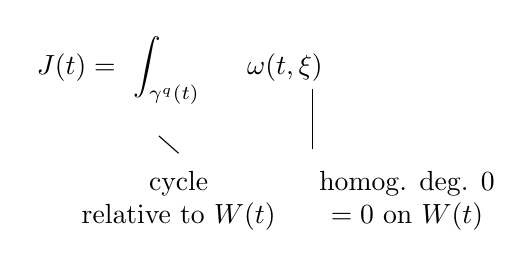
\begin{tikzpicture}[x=10mm, y=10mm, baseline=0pt]
\node[anchor=base] at (0,0) {$J (t)=$};
\node[anchor=base] at (1.15,0) {$\displaystyle\int_{\gamma^q (t)}$};
\node[anchor=base] at (2.65,0) {$\omega (t,\xi)$};
\draw (1.05,-0.78)--(1.30,-1.00);
\node[anchor=north] at (1.30,-1.10) {cycle};
\node[anchor=north] at (1.30,-1.50) {relative to $W (t)$};
\draw (3.00,-0.18)--(3.00,-0.95);
\node[anchor=north] at (4.20,-1.10) {homog. deg. $0$};
\node[anchor=north] at (4.20,-1.50) {$=0$ on $W (t)$};
\end{tikzpicture}
}}
\end{GelfandAdjacentEvidence}

$t\in T=C^n$,

$\xi\in C^{\ell+1}$



$\omega (t,\xi)$ on $P^\ell$, since it is homogeneous; the cycle is there too.





\SourcePage{GELFAND-P000224}{unlabelled}
$W (t)=\bigcup_k W_k (t)$ — hyperplanes, algebraic functions of $t$, singularities may occur (not in general position)



$t\in S_0[W]\Longleftrightarrow$ the dimension of the intersection of any number changes there.



\begin{GelfandAdjacentEvidence}{GELFAND-P000224}{1}
Def:
\begin{equation*}
 \gamma^{q-m}(t)=\bigcap_{j=1}^m V_j (t),
\end{equation*}
\Unclear{GELFAND-P000224}{intersection-sign}{Large sign: $\bigcap$ / $\bigwedge$; displayed candidate: $\bigcap$.}
\end{GelfandAdjacentEvidence}

\begin{center}
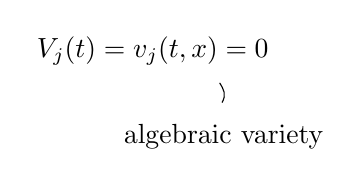
\begin{tikzpicture}[x=10mm, y=10mm, baseline=0pt]
\node[anchor=base] at (2.3,0) {$V_j (t)=v_j (t, x)=0$};
\draw (3.15,-0.32) .. controls (3.20,-0.40) and (3.24,-0.47) .. (3.18,-0.57);
\node[anchor=north] at (3.2,-0.72) {algebraic variety};
\end{tikzpicture}
\end{center}



\begin{GelfandAdjacentEvidence}{GELFAND-P000224}{2}

One must assume
\begin{equation*}
 \frac{\omega (t,\xi)}{[v_1(t,\xi)]^{1+\beta_1}\ldots[v_m]^{1+\beta_m}}
 \qquad\text{— defined on }P
\end{equation*}
\Unclear{GELFAND-P000224}{projective-rational-form}{The coordinate signs in the argument of $\omega$ and first denominator: $\xi$ / $s$; displayed candidate: $\xi$. The last factor is written $[v_m]^{1+\beta_m}$.}
\end{GelfandAdjacentEvidence}
\begin{GelfandAdjacentEvidence}{GELFAND-P000224}{3}

[On the left:] Residue
\begin{equation*}
 J (t)=\int_{\gamma^{q-m}(\xi)}
 \frac{d^{\beta_1+\ldots+\beta_m}\omega}
 {[dv_1]^{1+\beta_1}\wedge\ldots\wedge[dv_m]^{1+\beta_m}}
\end{equation*}
\Unclear{GELFAND-P000224}{residue-cycle-argument}{Argument below the integral: $\xi$ / $s$; displayed candidate: $\xi$.}
\end{GelfandAdjacentEvidence}




The singular support is also described in the general case

(On the covering space of the complement the form will be holomorphic)



\begin{GelfandAdjacentEvidence}{GELFAND-P000224}{4}
\underline{\underline{Thm.}} Then $J (t)$ has algebraic singular support.



\Unclear{GELFAND-P000224}{theorem-margin-note}{Right-margin note: “of type st. algebraic” / “of type sm. algebraic”; the first word and middle abbreviation are not uniquely established.}
\end{GelfandAdjacentEvidence}

(i.e. in $T$ there exists an algebraic variety such that $J (t)$ is holomorphic on a covering of the complement.)



Leray described the singular support in the case of planes.



$30/\underline{\overline{\mathrm{X}}}$\quad\underline{\underline{Sinai.}}
\begin{center}

\begin{tikzpicture}[x=10mm, y=10mm, baseline=0pt]
\node[anchor=base] at (2.6,0) {$U$-diffeom.};
\draw (0,-0.24) .. controls (0.16,-0.10) and (0.35,-0.10) .. (0.52,-0.24)
 .. controls (0.69,-0.38) and (0.87,-0.38) .. (1.04,-0.24)
 .. controls (1.21,-0.10) and (1.39,-0.10) .. (1.56,-0.24)
 .. controls (1.73,-0.38) and (1.91,-0.38) .. (2.08,-0.24)
 .. controls (2.25,-0.10) and (2.43,-0.10) .. (2.60,-0.24)
 .. controls (2.77,-0.38) and (2.95,-0.38) .. (3.12,-0.24)
 .. controls (3.29,-0.10) and (3.47,-0.10) .. (3.64,-0.24)
 .. controls (3.81,-0.38) and (3.99,-0.38) .. (4.16,-0.24)
 .. controls (4.33,-0.10) and (4.51,-0.10) .. (4.68,-0.24)
 .. controls (4.85,-0.38) and (5.03,-0.38) .. (5.20,-0.24);
\end{tikzpicture}
\end{center}




characteristic $\exp$ growth of the distance between nearby points (separation)

either as $t\longrightarrow+\infty$, or as $t\longrightarrow-\infty$.



\begin{equation*}
 \frac{d (T^n x, T^n y)}{d (x, y)}\geq ae^{cn}
 \qquad\begin{gathered}n>0\\\text{or }n<0\end{gathered}
 \qquad (x, y\text{ — nearby})
\end{equation*}



Consider the points $d (T^n y, T^n x)\leq ae^{-cn}d (y, x)$,



\begin{GelfandAdjacentEvidence}{GELFAND-P000224}{5}
Suppose that $\forall\ x$ this is a $k$-dimensional submanifold.







\SourceFigure{GELFAND-P000224}{manifold-sketch}{\par\smallskip\centering{\color{black}
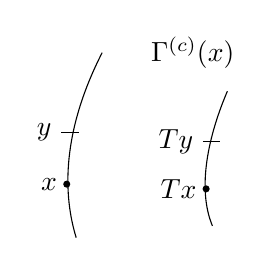
\begin{tikzpicture}[x=10mm, y=10mm]
\draw (0.15,0) .. controls (-0.05,0.65) and (0.02,1.45) .. (0.48,2.35);
\fill (0.03,0.68) circle (0.045);
\node[left] at (0.03,0.68) {$x$};
\draw (-0.04,1.34)--(0.19,1.34);
\node[left] at (-0.04,1.34) {$y$};
\draw (1.88,0.15) .. controls (1.68,0.63) and (1.83,1.3) .. (2.07,1.86);
\fill (1.8,0.62) circle (0.045);
\node[left] at (1.8,0.62) {$Tx$};
\draw (1.76,1.22)--(1.98,1.22);
\node[left] at (1.76,1.22) {$Ty$};
\node at (1.63,2.35) {$\Gamma^{(c)}(x)$};
\end{tikzpicture}
}}
\end{GelfandAdjacentEvidence}

This is a contracting submanifold (hence the index \underline{\underline{$c$}})



\begin{equation*}
 d (T^n y', T^n x)\leq ae^{+cn}d (y', x)
 \qquad (n\longrightarrow-\infty).
\end{equation*}



Similarly we obtain $\Gamma^{(p)}(x)$ — an expanding submanifold.

($\ell$-dimensional).



Then the choice does not depend on $a$ and $c$.





\SourcePage{GELFAND-P000225}{11}
$U$-system:
$k+\ell=n$ and the tangent spaces to the submanifolds are uniformly transverse



1. $k+\ell=n$

2. transversality.

3. Smoothness (not written out explicitly).



We obtain 2 foliations $\gamma^{(\mathrm{c})}$ and $\gamma^{(\mathrm{p})}$.



\begin{GelfandAdjacentEvidence}{GELFAND-P000225}{1}
\underline{Example:} linear transformation of the torus
$(x, y)\longrightarrow (ax+by, cx+dy)$.
\begin{equation*}
 \begin{vmatrix}a&b\\c&d\end{vmatrix}=1.
\end{equation*}





\Unclear{GELFAND-P000225}{lattice-diagram}{Two families of inclined lines and axes with arrows upwards and rightwards. The number of coinciding lines and continuations within dense crossings are not uniquely established. Individual lines have no labels.\par\smallskip\centering{\color{black}\begin{minipage}{68mm}\centering 
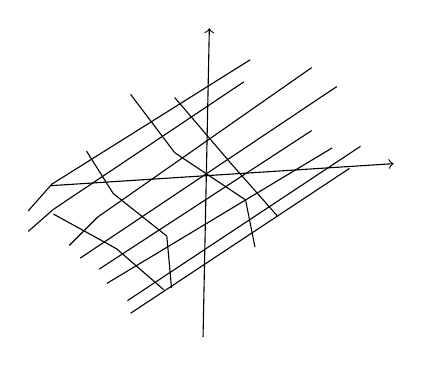
\begin{tikzpicture}[x=0.20mm, y=-0.20mm]
\draw (25,136)--(40,119)--(166,40);
\draw (25,149)--(41,135)--(162,54);
\draw (51,158)--(69,140)--(205,45);
\draw (58,166)--(221,57);
\draw (70,173)--(205,85);
\draw (75,182)--(218,96);
\draw (88,193)--(236,95);
\draw (90,201)--(229,109);
\draw (90,62)--(118,99)--(163,129)--(169,159);
\draw (118,64)--(153,105)--(183,139);
\draw (62,98)--(79,125)--(113,152)--(116,185);
\draw (41,138)--(81,160)--(111,186);
\draw[->] (136,216)--(140,20);
\draw[->] (39,120)--(257,106);
\end{tikzpicture}


(parallel to the eigendirections).
\end{minipage}}}
\end{GelfandAdjacentEvidence}

A nonlinear perturbation (periodic and smooth) is also a
$U$-diffeomorphism and the rotation number is the same.



\begin{center}

\begin{tikzpicture}[x=10mm, y=10mm, baseline=0pt]
\node[anchor=base] at (3.6,0) {Method of constructing $U$-diffeomorphisms.};
\draw (0,-0.24) .. controls (0.2,-0.07) and (0.4,-0.07) .. (0.6,-0.24)
 .. controls (0.8,-0.41) and (1.0,-0.41) .. (1.2,-0.24)
 .. controls (1.4,-0.07) and (1.6,-0.07) .. (1.8,-0.24)
 .. controls (2.0,-0.41) and (2.2,-0.41) .. (2.4,-0.24)
 .. controls (2.6,-0.07) and (2.8,-0.07) .. (3.0,-0.24)
 .. controls (3.2,-0.41) and (3.4,-0.41) .. (3.6,-0.24)
 .. controls (3.8,-0.07) and (4.0,-0.07) .. (4.2,-0.24)
 .. controls (4.4,-0.41) and (4.6,-0.41) .. (4.8,-0.24)
 .. controls (5.0,-0.07) and (5.2,-0.07) .. (5.4,-0.24)
 .. controls (5.6,-0.41) and (5.8,-0.41) .. (6.0,-0.24)
 .. controls (6.2,-0.07) and (6.4,-0.07) .. (6.6,-0.24)
 .. controls (6.8,-0.41) and (7.0,-0.41) .. (7.2,-0.24);
\end{tikzpicture}
\end{center}




$g$ — a Lie group, $\Gamma$ — a discrete subgroup.

\begin{GelfandAdjacentEvidence}{GELFAND-P000225}{2}
$g/\Gamma$ — compact.
\Unclear{GELFAND-P000225}{group-notation}{Lie-group notation: $g$ / $\mathfrak{G}$; displayed candidate: $g$, distinct from the subsequent $G$.}
\end{GelfandAdjacentEvidence}

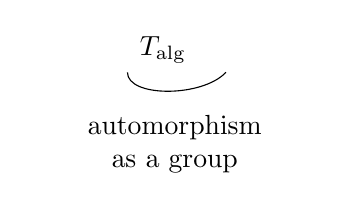
\begin{tikzpicture}[x=10mm, y=10mm, baseline=(symbol.base)]
\node (symbol) at (0,0) {$T_{\mathrm{alg}}$};
\draw (-0.45,-0.28) .. controls (-0.45,-0.60) and (0.50,-0.60) .. (0.80,-0.28);
\node[anchor=north, align=center, text width=35mm] at (0.15,-0.70) {automorphism as a group};
\end{tikzpicture}
 — an algebraic automorphism of $g$, leaving $\Gamma$ fixed
\quad$(T_{\mathrm{alg}}\Gamma=\Gamma)$



Then it acts on $g/\Gamma$.



Consider $G$ — the Lie algebra; $\hat T_{\mathrm{alg}}$ — the corresponding automorphism of $G$; if its

[At the left edge of the following line:] eigenvalues.



\begin{GelfandAdjacentEvidence}{GELFAND-P000225}{3}
Among them there are no
\Unclear{GELFAND-P000225}{cancelled-before-eigenvalues}{Crossed out: $\Longleftrightarrow$ / $\Longrightarrow$; endpoint directions are not established.}
\end{GelfandAdjacentEvidence}
\begin{GelfandAdjacentEvidence}{GELFAND-P000225}{4}

eigenvalues $=1$ in $\operatorname{mod}$



\Unclear{GELFAND-P000225}{terminal-arrow}{Sign after mod: $\Leftrightarrow$ / a crossed-out sign.}
\end{GelfandAdjacentEvidence}

$\Longleftrightarrow$ this is a $U$-diffeomorphism.



\begin{GelfandAdjacentEvidence}{GELFAND-P000225}{5}
(They exist $\Longleftrightarrow G$ is nilpotent).
\Unclear{GELFAND-P000225}{nilpotence-parenthesis}{Initial word in the parenthesis: “They exist” / “It exists”; the first candidate is displayed. The original fragment contains the entire parenthesis.}
\end{GelfandAdjacentEvidence}

Further. A small nonlinear perturbation $T=T_{\mathrm{alg}}+\Delta T$ is also a $U$-diffeomorphism.



\underline{Main problem:} topological similarity to the algebraic one.



For small perturbations — from Anosov's general theorem

(A small perturbation of a $U$-diffeomorphism is topologically similar to the original).



Always.
\begin{equation*}
 M=M_1\cup M_2
\end{equation*}



$M_2$ — wandering points



$M_1$ — nonwandering points. — the condition $U$ holds on them



[In the right margin:]
\begin{center}
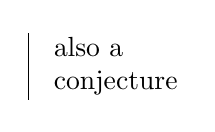
\begin{tikzpicture}[x=10mm, y=10mm]
\draw (0,0)--(0,0.85);
\node[anchor=west, align=left] at (0.2,0.43) {also a\\conjecture};
\end{tikzpicture}
\end{center}






\begin{GelfandAdjacentEvidence}{GELFAND-P000226}{1}
\SourcePage{GELFAND-P000226}{unlabelled}
An important construction:







\SourceFigure{GELFAND-P000226}{holonomy-diagram}{\par\smallskip\centering{\color{black}
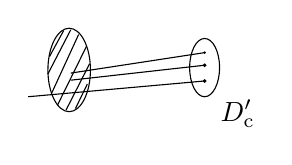
\begin{tikzpicture}[x=10mm, y=10mm]
\draw (0,0) ellipse (0.27 and 0.53);
\draw (-0.22,-0.29)--(0.12,0.45);
\draw (-0.27,-0.05)--(0.02,0.51);
\draw (-0.25,0.17)--(-0.07,0.50);
\draw (-0.15,-0.45)--(0.22,0.30);
\draw (-0.04,-0.51)--(0.26,0.08);
\draw (0.08,-0.49)--(0.23,-0.18);
\draw (1.72,0.03) ellipse (0.19 and 0.37);
\draw (0.02,-0.04)--(1.72,0.22);
\draw (0.02,-0.13)--(1.72,0.06);
\draw (-0.52,-0.34)--(1.72,-0.14);
\fill (1.72,0.22) circle (0.018);
\fill (1.72,0.06) circle (0.025);
\fill (1.72,-0.14) circle (0.025);
\node[below right] at (1.80,-0.26) {$D'_{\mathrm{c}}$};
\end{tikzpicture}
}}
\end{GelfandAdjacentEvidence}

natural isomorphism of our pieces. of contracting leaves (along noncontracting leaves).



$D_{\mathrm{c}}$ — a contracting submanifold, $\dim=k$.



($\pi$ — the canonical isomorphism.)



\begin{GelfandAdjacentEvidence}{GELFAND-P000226}{2}
$\pi$ is not always smooth (!), but it is absolutely continuous, i.e. the natural measures pass into one another.





\Unclear{GELFAND-P000226}{parallelogram-diagram}{Two nearly vertical curved strokes and transverse curves; the number of coinciding strokes and their continuations at the dense middle crossings are not uniquely established. No labels or arrows are visible.\par\smallskip\centering{\color{black}\begin{minipage}{68mm}\centering A parallelogram:
\begin{center}
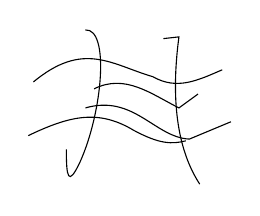
\begin{tikzpicture}[x=0.22mm, y=-0.22mm]
\draw (80,28) .. controls (94,27) and (90,75) .. (77,104)
 .. controls (70,119) and (69,113) .. (69,97);
\draw (125,33)--(134,32) .. controls (130,62) and (131,94) .. (146,117);
\draw (50,58) .. controls (79,34) and (95,48) .. (119,55)
 .. controls (133,63) and (145,57) .. (159,51);
\draw (85,62) .. controls (103,53) and (118,65) .. (134,73)--(145,65);
\draw (80,73) .. controls (108,65) and (120,90) .. (140,91)--(164,81);
\draw (47,89) .. controls (72,77) and (88,74) .. (108,86)
 .. controls (123,94) and (130,94) .. (138,92);
\end{tikzpicture}
\end{center}

made of segments of foliations
\end{minipage}}}
\end{GelfandAdjacentEvidence}

(all its leaves are canonically isomorphic: both contracting and expanding.)



\begin{equation*}
 \Gamma (U)=\Gamma_{\mathrm{p}}(U)\cup\Gamma_{\mathrm{c}}(U)
\end{equation*}



Suppose there is a system of parallelograms $U_i$ adjoining one another.



\begin{equation*}
 \begin{gathered}
 M=\bigcup\overline{U}_i\\
 U_i\cap U_j\subset\Gamma (U_i)\cap\Gamma (U_j)
 \end{gathered}
 \qquad (\Gamma\text{ — boundaries}).
\end{equation*}



$\alpha$ — such a partition into parallelograms. Consider the boundaries:



\begin{equation*}
 \begin{gathered}
 \Gamma_{\mathrm{p}}(\alpha)=\bigcup_i\Gamma_{\mathrm{p}}(U_i)\\
 \Gamma_{\mathrm{c}}(\alpha)=\bigcup_i\Gamma_{\mathrm{c}}(U_i)
 \end{gathered}
\end{equation*}



\begin{GelfandAdjacentEvidence}{GELFAND-P000226}{3}
[Drawing on the right:]




\SourceFigure{GELFAND-P000226}{boundary-diagram}{\par\smallskip\centering{\color{black}
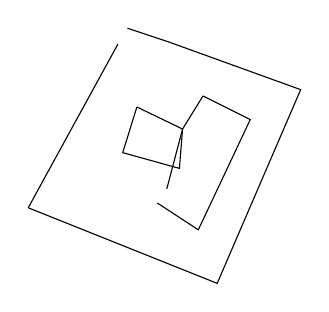
\begin{tikzpicture}[x=0.20mm, y=-0.20mm]
\draw (25,142)--(82,38);
\draw (88,28)--(115,37)--(198,67)--(145,190)--(25,142);
\draw (136,71)--(166,86)--(133,156)--(107,139);
\draw (113,130)--(123,92)--(136,71);
\draw (94,78)--(85,107)--(121,117)--(123,92)--(94,78);
\end{tikzpicture}
}}
\end{GelfandAdjacentEvidence}

This $\alpha$ is called Markov if there exists an $m$ such that



\begin{equation*}
 \fbox{$\begin{gathered}
 \Gamma_{\mathrm{p}}(T^{-m}\alpha)\subset\Gamma_{\mathrm{p}}(\alpha)\\
 \Gamma_{\mathrm{c}}(T^{+m}\alpha)\subset\Gamma_{\mathrm{c}}(\alpha)
 \end{gathered}$}
\end{equation*}



\begin{center}
\begin{tikzpicture}[x=10mm, y=10mm]
\node[anchor=north west, align=left, text width=126mm, inner sep=2mm] (statement) at (0,0) {\underline{Thm.} (technical) Markov partitions exist and there are many of them: $\forall$ \begin{tikzpicture}[x=10mm, y=10mm, baseline=(parameter.base)]
\node (parameter) at (0,0) {$\alpha$};
\draw (-0.02,-0.23)--(-0.22,-0.70);
\node[anchor=north, align=center] at (-0.22,-0.78) {partition into\\parallelograms};
\end{tikzpicture}, $\forall\varepsilon>0$ $\exists m$ and a partition $\widetilde\alpha$, such that it will be at a distance of less than $\varepsilon$ from the original.};
\draw (statement.north east)--(statement.north west)--++(-0.35,0)--++(0,-0.45)--++(-0.65,0)--++(0,-1.15)--++(0.65,0) |- (statement.south west)--(statement.south east);
\end{tikzpicture}
\end{center}



\begin{GelfandAdjacentEvidence}{GELFAND-P000226}{4}

[On the left:]




\Unclear{GELFAND-P000226}{bottom-diagrams}{A separate inclined quadrilateral and a narrow inclined strip with transverse quadrilaterals at its ends. The continuations of several superposed contours at the upper right end are not uniquely established. There are no arrows.\par\smallskip\centering{\color{black}
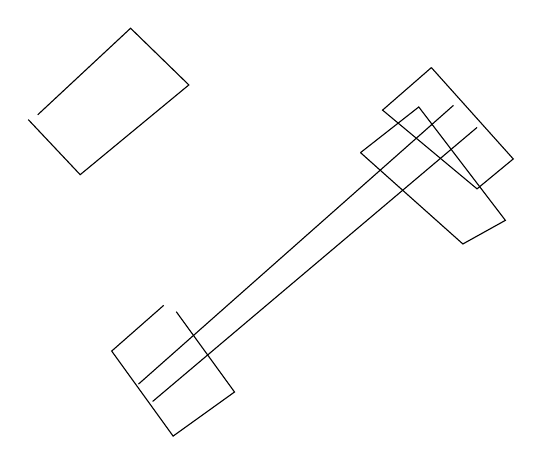
\begin{tikzpicture}[x=0.20mm, y=-0.20mm]
\draw (32,92)--(91,37)--(128,73)--(59,130)--(26,95);
\draw (96,263)--(296,86);
\draw (105,274)--(311,100);
\draw (282,62)--(334,120)--(311,139)--(251,89)--(282,62);
\draw (237,116)--(274,87)--(329,159)--(302,174)--(237,116);
\draw (112,213)--(79,242)--(118,296)--(157,268)--(120,217);
\end{tikzpicture}
}}
\end{GelfandAdjacentEvidence}

the ends cannot be in the middle.

(original parallelogram.)



\begin{center}$\text{—}\,\bullet\,\text{—}$\end{center}



If $\alpha$ is a partition with $m$, then one can make $m=1$, taking the intersection



\begin{equation*}
 \alpha_1=\alpha\cdot T^{-1}\alpha\cdots\cdot T^{-m+1}\alpha\;\text{—}
\end{equation*}
— Markov with $m=1$





\SourcePage{GELFAND-P000227}{12}
— from
\begin{equation*}
 \Gamma_{\mathrm{p}}(\alpha_1)=\Gamma_{\mathrm{p}}(\alpha)
 \cup\Gamma_{\mathrm{p}}(T^{-1}\alpha)\cup\cdots
 \cup\Gamma_{\mathrm{p}}(T^{-m+1}\alpha)
\end{equation*}



\begin{center}

\begin{tikzpicture}[x=1mm, y=1mm]
\node[anchor=base, align=left, text width=136mm] at (70.0,0) {Symbolic dynamics for a $U$-diffeomorphism.};
\draw (0,-2) .. controls (2,-1) and (4,-1) .. (6,-2)
 .. controls (8,-3) and (10,-3) .. (12,-2)
 .. controls (14,-1) and (16,-1) .. (18,-2)
 .. controls (20,-3) and (22,-3) .. (24,-2)
 .. controls (26,-1) and (28,-1) .. (30,-2)
 .. controls (32,-3) and (34,-3) .. (36,-2)
 .. controls (38,-1) and (40,-1) .. (42,-2)
 .. controls (44,-3) and (46,-3) .. (48,-2)
 .. controls (50,-1) and (52,-1) .. (54,-2)
 .. controls (56,-3) and (58,-3) .. (60,-2)
 .. controls (62,-1) and (64,-1) .. (66,-2)
 .. controls (68,-3) and (70,-3) .. (72,-2)
 .. controls (74,-1) and (76,-1) .. (78,-2)
 .. controls (80,-3) and (82,-3) .. (84,-2)
 .. controls (86,-1) and (88,-1) .. (90,-2)
 .. controls (92,-3) and (94,-3) .. (96,-2)
 .. controls (98,-1) and (100,-1) .. (102,-2)
 .. controls (104,-3) and (106,-3) .. (108,-2)
 .. controls (110,-1) and (112,-1) .. (114,-2)
 .. controls (116,-3) and (118,-3) .. (120,-2)
 .. controls (122,-1) and (124,-1) .. (126,-2)
 .. controls (128,-3) and (130,-3) .. (132,-2)
 .. controls (134,-1) and (136,-1) .. (138,-2);
\end{tikzpicture}
\end{center}




(Suppose there is a Markov partition and with $m=1$.)



\begin{equation*}
 \pi_{j_1j_2}=\begin{cases}
 1&V_{j_1}\cap TV_{j_2}\ne\varnothing\\
 0&\text{in the remaining cases}
 \end{cases}
\end{equation*}
\Needspace{8\baselineskip}
$\Pi$\par\nobreak



$\Omega_\Pi$ — the space of points
\begin{equation*}
 \begin{gathered}
 \omega=\{\ldots\ j_{-n},\ldots, j_0,\ldots, j_n,\ldots\}\\
 \pi_{j_nj_{n+1}}=1.
 \end{gathered}
\end{equation*}



Now associate
\begin{equation*}
 \omega\longrightarrow\bigcap_{-\infty}^{+\infty}T^n\overline{V}_{j_n}
 =x\in M\qquad (!)
\end{equation*}



(nonempty by the Markov property and, for a fine partition, consists of 1 point.)



We obtain a map $\varphi:\Omega_\Pi\longrightarrow M$



[A parenthesis begun on the right:] (from nonuniqueness.



\begin{GelfandAdjacentEvidence}{GELFAND-P000227}{1}
it is not
\Unclear{GELFAND-P000227}{overwritten-negation}{After the readable “not” a short entry is crossed out; possible “one-to-” is not established.}
\end{GelfandAdjacentEvidence}

one-to-one because of the points — boundaries of parallelograms).

On a set of the 2nd category it is one-to-one.



\underline{Condition:} $\Pi^K$ consists of positive entries for some $K$.



(i.e. all leaves $\Gamma^{(\mathrm{c})}$ and $\Gamma^{(\mathrm{p})}$ are dense in $M$ — this is necessary and sufficient.)



\begin{center}

\begin{tikzpicture}[x=1mm, y=1mm]
\node[anchor=base, align=left, text width=136mm] at (70.0,0) {On each leaf $\Gamma^{(\mathrm{c})}$ a $\sigma$-finite measure $\lambda_{\mathrm{c}}$ is introduced,};
\draw (0,-2) .. controls (2,-1) and (4,-1) .. (6,-2)
 .. controls (8,-3) and (10,-3) .. (12,-2)
 .. controls (14,-1) and (16,-1) .. (18,-2)
 .. controls (20,-3) and (22,-3) .. (24,-2)
 .. controls (26,-1) and (28,-1) .. (30,-2)
 .. controls (32,-3) and (34,-3) .. (36,-2)
 .. controls (38,-1) and (40,-1) .. (42,-2)
 .. controls (44,-3) and (46,-3) .. (48,-2)
 .. controls (50,-1) and (52,-1) .. (54,-2)
 .. controls (56,-3) and (58,-3) .. (60,-2)
 .. controls (62,-1) and (64,-1) .. (66,-2)
 .. controls (68,-3) and (70,-3) .. (72,-2)
 .. controls (74,-1) and (76,-1) .. (78,-2)
 .. controls (80,-3) and (82,-3) .. (84,-2)
 .. controls (86,-1) and (88,-1) .. (90,-2)
 .. controls (92,-3) and (94,-3) .. (96,-2)
 .. controls (98,-1) and (100,-1) .. (102,-2)
 .. controls (104,-3) and (106,-3) .. (108,-2)
 .. controls (110,-1) and (112,-1) .. (114,-2)
 .. controls (116,-3) and (118,-3) .. (120,-2)
 .. controls (122,-1) and (124,-1) .. (126,-2)
 .. controls (128,-3) and (130,-3) .. (132,-2)
 .. controls (134,-1) and (136,-1) .. (138,-2);
\end{tikzpicture}
\end{center}

\begin{GelfandAdjacentEvidence}{GELFAND-P000227}{2}
where

[On the left:]




\Unclear{GELFAND-P000227}{invariant-measure-diagram}{The lines labelled $A,\widetilde A$ and connecting curves. Directed thickenings are visible at two lower right ends; the number of coinciding lower curves and character of the other ends are not uniquely established.\par\smallskip\centering{\color{black}
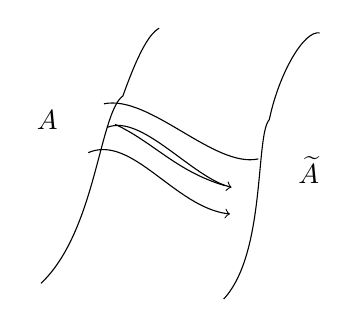
\begin{tikzpicture}[x=0.20mm, y=-0.20mm]
\draw (30,194) .. controls (65,161) and (67,86) .. (82,75)
 .. controls (91,50) and (98,36) .. (105,32);
\draw (146,204) .. controls (173,175) and (166,100) .. (175,90)
 .. controls (181,61) and (197,33) .. (207,35);
\node at (34,90) {$A$};
\node at (200,122) {$\widetilde A$};
\draw (70,80) .. controls (99,74) and (140,121) .. (168,115);
\draw[->] (72,95) .. controls (94,86) and (126,127) .. (151,133);
\draw (77,93) .. controls (101,104) and (116,123) .. (147,132);
\draw[->] (60,111) .. controls (88,99) and (115,146) .. (150,150);
\end{tikzpicture}
}}
\end{GelfandAdjacentEvidence}

1) $\lambda_{\mathrm{c}}(A)=\lambda_{\mathrm{c}}(\widetilde A)$

(measures of canonically isomorphic sets are equal.)

2) $\lambda_{\mathrm{c}}(TA)=h\lambda_{\mathrm{c}}(A)$\quad$(h<1)$

($h$ — an algebraic number.)



— additional information.

(Reflects the homogeneous structure.)



\begin{GelfandAdjacentEvidence}{GELFAND-P000227}{3}
(In an algebraic
\Unclear{GELFAND-P000227}{cancelled-group-word}{A word is crossed out, possibly “case”; its reading is not established.}
[Inserted above:] $U$-automorphism
everything is induced by Haar measure.)
\end{GelfandAdjacentEvidence}



\begin{GelfandAdjacentEvidence}{GELFAND-P000227}{4}
\begin{center}

\begin{tikzpicture}[x=1mm, y=1mm]
\node[anchor=base, align=left, text width=38mm] at (21.0,0) {Corollary:};
\draw (0,-2) .. controls (2,-1) and (4,-1) .. (6,-2)
 .. controls (8,-3) and (10,-3) .. (12,-2)
 .. controls (14,-1) and (16,-1) .. (18,-2)
 .. controls (20,-3) and (22,-3) .. (24,-2)
 .. controls (26,-1) and (28,-1) .. (30,-2)
 .. controls (32,-3) and (34,-3) .. (36,-2)
 .. controls (38,-1) and (40,-1) .. (42,-2);
\end{tikzpicture}
\end{center}
 there is an invariant measure, $T$ is
\Unclear{GELFAND-P000227}{cancelled-before-chain}{Crossed-out sign: Cyrillic “б” / “в”; its reading is not established.}
\end{GelfandAdjacentEvidence}

a finite Markov chain.



\begin{GelfandAdjacentEvidence}{GELFAND-P000227}{5}
\begin{center}

\begin{tikzpicture}[x=1mm, y=1mm]
\node[anchor=base, align=left, text width=86mm] at (45.0,0) {Construction of this measure:};
\draw (0,-2) .. controls (2,-1) and (4,-1) .. (6,-2)
 .. controls (8,-3) and (10,-3) .. (12,-2)
 .. controls (14,-1) and (16,-1) .. (18,-2)
 .. controls (20,-3) and (22,-3) .. (24,-2)
 .. controls (26,-1) and (28,-1) .. (30,-2)
 .. controls (32,-3) and (34,-3) .. (36,-2)
 .. controls (38,-1) and (40,-1) .. (42,-2)
 .. controls (44,-3) and (46,-3) .. (48,-2)
 .. controls (50,-1) and (52,-1) .. (54,-2)
 .. controls (56,-3) and (58,-3) .. (60,-2)
 .. controls (62,-1) and (64,-1) .. (66,-2)
 .. controls (68,-3) and (70,-3) .. (72,-2)
 .. controls (74,-1) and (76,-1) .. (78,-2)
 .. controls (80,-3) and (82,-3) .. (84,-2)
 .. controls (86,-1) and (88,-1) .. (90,-2);
\end{tikzpicture}
\end{center}
 $(n=2)$







\Unclear{GELFAND-P000227}{final-diagrams}{Two diagrams with $V_i$, leader stroke, transverse marks, and visible directed strokes. Connections of thick lines at the base of the right diagram and some endpoint directions remain undetermined. There is no arrow between the diagrams.\par\smallskip\centering{\color{black}
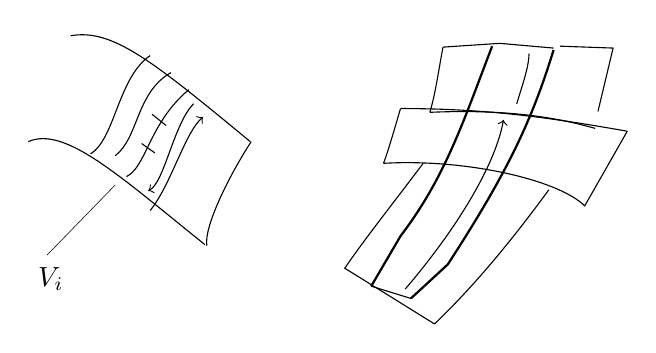
\begin{tikzpicture}[x=0.12mm, y=-0.12mm]
\draw (63,18) .. controls (107,10) and (150,45) .. (253,130);
\draw (18,130) .. controls (57,113) and (115,167) .. (205,239);
\draw (254,130) .. controls (230,167) and (204,220) .. (207,240);
\draw (84,143) .. controls (110,127) and (113,62) .. (147,39);
\draw (110,145) .. controls (135,126) and (132,78) .. (169,57);
\draw (122,167) .. controls (143,157) and (146,110) .. (188,75);
\draw (138,132)--(152,142);
\draw (149,101)--(164,113);
\draw[->] (193,90) .. controls (172,111) and (162,174) .. (145,182);
\draw[->] (147,203) .. controls (169,176) and (184,120) .. (203,104);
\draw[line width=0.2pt] (38,250)--(110,176);
\node[below] at (42,253) {$V_i$};
\begin{scope}[xshift=40.44mm]
\draw (120,30)--(180,26)--(237,31);
\draw (244,29)--(300,31)--(284,98);
\draw (106,99) .. controls (112,80) and (116,50) .. (120,30);
\draw (106,99) .. controls (197,95) and (249,107) .. (281,116);
\draw (75,95) .. controls (70,112) and (62,140) .. (57,153);
\draw (75,95) .. controls (169,95) and (235,105) .. (315,119);
\draw (57,153) .. controls (140,148) and (240,169) .. (270,198)--(315,119);
\draw[line width=0.8pt] (172,29) .. controls (142,107) and (123,167) .. (75,230)--(44,283);
\draw[line width=0.8pt] (237,33) .. controls (214,108) and (188,163) .. (125,260)--(86,296);
\draw (99,153) .. controls (65,198) and (35,236) .. (16,264)--(111,323);
\draw (111,323) .. controls (158,278) and (199,226) .. (232,181);
\draw (44,283)--(86,296);
\draw[->] (80,286) .. controls (124,235) and (174,162) .. (184,107);
\draw (198,90) .. controls (203,73) and (211,51) .. (211,37);
\end{scope}
\end{tikzpicture}
}}
\end{GelfandAdjacentEvidence}
\begin{GelfandAdjacentEvidence}{GELFAND-P000227}{6}

\begin{equation*}
 \lambda_i h^{-1}=\sum\lambda_i'=\sum\pi_{ii'}\lambda_{i'},\quad\text{i.e.}
\end{equation*}
\Unclear{GELFAND-P000227}{first-sum-prime}{In the first sum the prime is high: $\sum\lambda_i'$ / $\sum\lambda_{i'}$; the first candidate is displayed.}
\end{GelfandAdjacentEvidence}

\begin{equation*}
 \fbox{$h^{-1}\vec\lambda=\Pi\vec\lambda$.}
\end{equation*}
— eigenvector.



\begin{GelfandAdjacentEvidence}{GELFAND-P000227}{7}
(This is for our
\Unclear{GELFAND-P000227}{bottom-cancelled-word}{A short crossed-out entry is illegible.}


parallelograms).



The values of the measure on a segment are given. Then from the 2nd property.

[Below the last line:] (on a smaller segment.)
\end{GelfandAdjacentEvidence}







\begin{GelfandAdjacentEvidence}{GELFAND-P000228}{1}
\SourcePage{GELFAND-P000228}{unlabelled}
\Unclear{GELFAND-P000228}{title-ending}{Энтропия / Энтропии (entropy); the ending is not uniquely established.}


\begin{equation*}
 T=\left|\begin{array}{ccc}a&\cdot&b\\c&&d\end{array}\right|
\end{equation*}



\begin{equation*}
 h (T)=\ln\lambda\quad (\lambda>1)
\end{equation*}



\begin{equation*}
 h (T)=\lambda
\end{equation*}
\end{GelfandAdjacentEvidence}



$\Rightarrow$ the transformations are metrically isomorphic.

\begin{GelfandAdjacentEvidence}{GELFAND-P000228}{2}
$\Omega_{\Pi_1}$ maps onto $\Omega_{\Pi_0}$ (stand.) —



\Unclear{GELFAND-P000228}{earlier-abbreviation}{прежн. раз. / прим. раз. (prev. time / example, time); the first abbreviation is undetermined.}
\end{GelfandAdjacentEvidence}


And it remains to map the torus onto $\Omega_{\Pi_1}$.

\begin{GelfandAdjacentEvidence}{GELFAND-P000228}{3}
$\Pi_1$ is of a certain type: 4 groups of letters and properties
of transitions — see earlier.







\Unclear{GELFAND-P000228}{torus-partition}{A nearly rectangular frame, oblique edges projecting above, to the right and below, and hatching. Continuations of lines at dense crossings and exact boundaries of the hatched parts are not uniquely established. There are no vertex labels or arrows.\par\smallskip\centering{\color{black}\GelfandFitDiagram{
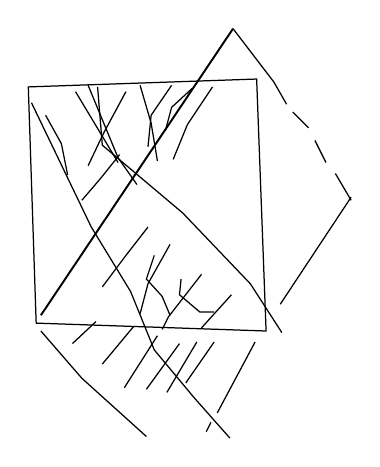
\begin{tikzpicture}[x=0.20mm, y=-0.20mm, line width=0.45pt]
\draw (30,55)--(175,50)--(181,210)--(35,205)--cycle;
\draw[line width=0.7pt] (38,200)--(160,18);
\draw (32,65)--(70,144)--(95,185)--(110,222)--(135,252)--(158,278);
\draw (74,55)--(77,92)--(128,135)--(171,180)--(191,211);
\draw (160,18)--(186,52)--(194,66);
\draw (198,71)--(208,81);
\draw (212,89)--(219,103);
\draw (225,110)--(235,127);
\draw (235,125)--(190,193);
\draw (38,210)--(64,240)--(105,277);
\draw (150,262)--(174,217);
\draw (146,268)--(143,274);
\draw (60,58)--(72,78)--(87,103);
\draw (41,73)--(51,91)--(55,111);
\draw (68,54)--(87,100)--(99,117);
\draw (101,54)--(108,78)--(112,102);
\draw (121,54)--(108,73)--(106,93);
\draw (92,58)--(78,84)--(68,105);
\draw (147,55)--(131,79)--(122,101);
\draw (134,56)--(121,68)--(117,83);
\draw (88,98)--(76,113)--(64,127);
\draw (106,144)--(92,162)--(77,182);
\draw (120,155)--(106,180)--(101,199);
\draw (140,174)--(119,201)--(115,209);
\draw (159,187)--(140,208);
\draw (110,162)--(105,177)--(115,188)--(120,200);
\draw (127,177)--(126,187)--(139,198)--(148,198);
\draw (58,218)--(73,204);
\draw (77,231)--(97,207);
\draw (91,246)--(112,213);
\draw (105,247)--(126,218);
\draw (118,249)--(137,217);
\draw (130,243)--(148,217);
\end{tikzpicture}
}}\par\smallskip}
\end{GelfandAdjacentEvidence}

— a partition of the torus into 2 parallelograms
(the sides $\parallel$ the eigendirections)



\begin{GelfandAdjacentEvidence}{GELFAND-P000228}{4}

The sides lie on a line through 0
in an eigendirection (and \Unclear{GELFAND-P000228}{parenthetical-direction}{продолж. / проек. (cont. / proj.); the middle strokes of the abbreviation merge.}

).
\end{GelfandAdjacentEvidence}

This is a Markov partition (the coarsest).
It is because of it that one succeeds in solving the isomorphism problem.



\begin{GelfandAdjacentEvidence}{GELFAND-P000228}{5}

\begin{equation*}
 \bigcap T^n V_{\omega_n}
\end{equation*}
\Unclear{GELFAND-P000228}{intersection-subscript}{The subscript under $V$ is $\omega_n$ / $\omega$; a separate lower $n$ is not established. No separate index is visible at the intersection sign.}


may consist of a large number of points.
\end{GelfandAdjacentEvidence}

\begin{GelfandAdjacentEvidence}{GELFAND-P000228}{6}
Consider first 4 parallelograms:
\begin{gather*}
 V_1\cap TV_1\\
 V_2\cap TV_2\\
 V_1\cap TV_2\\
 V_1\cap TV_2
\end{gather*}



\Unclear{GELFAND-P000228}{second-pair}{The second intersection: $V_2\cap TV_2$ / $V_2\cap TV_1$. The right subscript is heavily retraced; the first candidate is displayed.}
\end{GelfandAdjacentEvidence}




\begin{GelfandAdjacentEvidence}{GELFAND-P000228}{7}

(\Unclear{GELFAND-P000228}{uzhe-cancellation}{Уже (Already); the word is readable, but whether a transverse stroke crosses it out is undetermined.}
 a disconnected partition. Form a partition —
— its connected components. Their numbers, respectively —
— \Unclear{GELFAND-P000228}{component-counts}{$p, q, r, s$; the second sign is heavily retraced and $q$ remains a candidate.}

)
\end{GelfandAdjacentEvidence}





\begin{GelfandAdjacentEvidence}{GELFAND-P000229}{91}
\SourcePage{GELFAND-P000229}{unlabelled}
\underline{\underline{Year 1968.}}

12/\underline{II}\quad\underline{Question} (Gelfand)



$R$ — a countably normed ring:




\begin{equation*}
 \lVert xy\rVert_i\leq\lVert x\rVert_k\lVert y\rVert_\ell
\end{equation*}
\Unclear{GELFAND-P000229}{norm-final-index}{The last subscript: $\ell$ / $e$; $\ell$ is displayed.}

\end{GelfandAdjacentEvidence}
\begin{GelfandAdjacentEvidence}{GELFAND-P000229}{2}





\SourceFigure{GELFAND-P000229}{stepped-theorem-frame}{\par\smallskip\centering{\color{black}\GelfandFitDiagram{
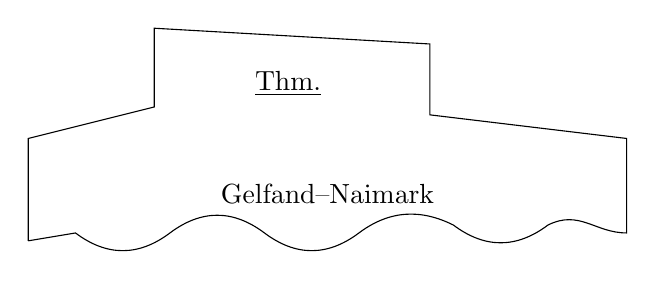
\begin{tikzpicture}[x=1mm, y=1mm]
\draw (0,0)--(0,13)--(16,17)--(16,27)--(51,25)--(51,16)--(76,13)--(76,1)
 .. controls (72,1) and (70,4) .. (66,2)
 .. controls (62,-1) and (58,-1) .. (54,2)
 .. controls (50,4) and (46,4) .. (42,1)
 .. controls (38,-2) and (34,-2) .. (30,1)
 .. controls (26,4) and (22,4) .. (18,1)
 .. controls (14,-2) and (10,-2) .. (6,1)--(0,0);
\node at (33,20) {\underline{Thm.}};
\node at (38,6) {Gelfand–Naimark};
\end{tikzpicture}
}}\par\smallskip}
\end{GelfandAdjacentEvidence}
\begin{GelfandAdjacentEvidence}{GELFAND-P000229}{92}


for \Unclear{GELFAND-P000229}{superscribed-mark}{[Superscribed sign: superposed loops and strokes; its reading is undetermined.]}



normed rings:
\begin{equation*}
 f (x^*x)\geq0\Rightarrow f (x)=\int_{\mathcal M_0}x (M)\, d\sigma (M)
\end{equation*}
($\mathcal M_0$ — symm. ideals)
\Unclear{GELFAND-P000229}{ideal-space-notation}{In the lower limit and the explanation, the letter is $M_0$ / $m_0$ / $\mathcal M_0$; the lower zero is readable. Case and style are undetermined; $\mathcal M_0$ is displayed.}

\end{GelfandAdjacentEvidence}

Extension — ? (Not always: one must
characterize the class axiomatically).



\begin{equation*}
 x^*(M)=\overline{x (M')},\quad M=M'
\end{equation*}
— symm.



$L^1$ with convolution, $\overline{x (-t)}=x^*(t)$



$\Rightarrow$ Bochner's theorem
\begin{equation*}
 \int_{-\infty}^{+\infty}e^{it\lambda}\, d\sigma (t)
\end{equation*}



\begin{GelfandAdjacentEvidence}{GELFAND-P000229}{5}
\underline{\underline{I. Bernstein.}}




\SourceFigure{GELFAND-P000229}{topology-heading}{\par\smallskip\centering{\color{black}\GelfandFitDiagram{

\begin{tikzpicture}[x=1mm, y=1mm]
\node[anchor=base] at (69,0) {Grothendieck topology.};
\draw (0,-2) .. controls (2,-1) and (4,-1) .. (6,-2)
 .. controls (8,-3) and (10,-3) .. (12,-2)
 .. controls (14,-1) and (16,-1) .. (18,-2)
 .. controls (20,-3) and (22,-3) .. (24,-2)
 .. controls (26,-1) and (28,-1) .. (30,-2)
 .. controls (32,-3) and (34,-3) .. (36,-2)
 .. controls (38,-1) and (40,-1) .. (42,-2)
 .. controls (44,-3) and (46,-3) .. (48,-2)
 .. controls (50,-1) and (52,-1) .. (54,-2)
 .. controls (56,-3) and (58,-3) .. (60,-2)
 .. controls (62,-1) and (64,-1) .. (66,-2)
 .. controls (68,-3) and (70,-3) .. (72,-2)
 .. controls (74,-1) and (76,-1) .. (78,-2)
 .. controls (80,-3) and (82,-3) .. (84,-2)
 .. controls (86,-1) and (88,-1) .. (90,-2)
 .. controls (92,-3) and (94,-3) .. (96,-2)
 .. controls (98,-1) and (100,-1) .. (102,-2)
 .. controls (104,-3) and (106,-3) .. (108,-2)
 .. controls (110,-1) and (112,-1) .. (114,-2)
 .. controls (116,-3) and (118,-3) .. (120,-2)
 .. controls (122,-1) and (124,-1) .. (126,-2)
 .. controls (128,-3) and (130,-3) .. (132,-2)
 .. controls (134,-1) and (136,-1) .. (138,-2);
\end{tikzpicture}
}}\par\smallskip}
\end{GelfandAdjacentEvidence}

$T$ is the following collection:

1) The category $\operatorname{Cat}T$ is specified (objects — open sets).

2) Certain families $\{\alpha_i: U_i\to U\}$ are specified,
called coverings

\begin{GelfandAdjacentEvidence}{GELFAND-P000229}{93}
3) A system satisfying axioms is specified:




1. There exists an intersection — a \underline{product} (fibered).




\SourceFigure{GELFAND-P000229}{fiber-product-diagram}{\par\smallskip\centering{\color{black}\GelfandFitDiagram{
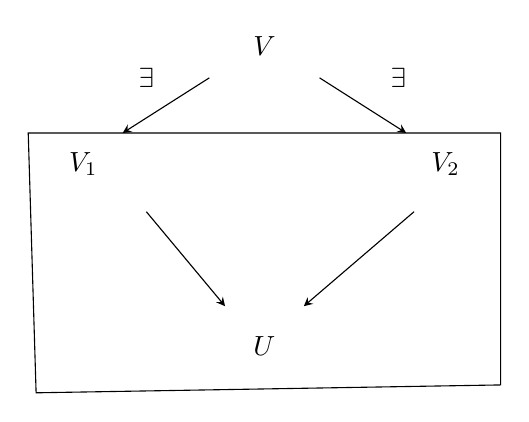
\begin{tikzpicture}[x=1mm, y=1mm,>=stealth]
\node at (30,38) {$V$};
\node at (7,23) {$V_1$};
\node at (53,23) {$V_2$};
\node at (30,0) {$U$};
\draw[->] (23,34)--(12,27);
\draw[->] (37,34)--(48,27);
\node at (15,34) {$\exists$};
\node at (47,34) {$\exists$};
\draw[->] (15,17)--(25,5);
\draw[->] (49,17)--(35,5);
\draw (0,27)--(60,27)--(60,-5)--(1,-6)--cycle;
\end{tikzpicture}
}}\par\smallskip}



(commut.).




\SourceFigure{GELFAND-P000229}{given-data-caption}{\par\smallskip\centering{\color{black}\GelfandFitDiagram{
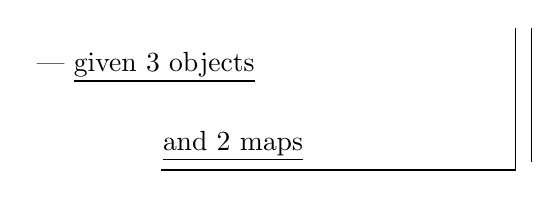
\begin{tikzpicture}[x=1mm, y=1mm]
\node[anchor=west] at (0,10) {— \underline{given 3 objects}};
\node[anchor=west] at (16,0) {\underline{and 2 maps}};
\draw (17,-3)--(62,-3)--(62,15);
\draw (64,-2)--(64,15);
\end{tikzpicture}
}}\par\smallskip}

\end{GelfandAdjacentEvidence}
\begin{GelfandAdjacentEvidence}{GELFAND-P000229}{8}

\fbox{$V=V_1\times_U V_2$} — notation.
Then there exists







\SourceFigure{GELFAND-P000229}{open-set-sketch}{\par\smallskip\centering{\color{black}\GelfandFitDiagram{
\begin{tikzpicture}[x=1mm, y=1mm]
\draw (15,15) .. controls (-11,4) and (-22,-17) .. (2,-29)
 .. controls (23,-39) and (49,-18) .. (49,3)
 .. controls (49,17) and (36,23) .. (24,18);
\draw[rotate=32] (6,-5) ellipse (9mm and 5mm);
\draw[rotate=32] (15,-3) ellipse (9mm and 7mm);
\draw (12,-6)--(15,2);
\node at (65,-4) {$U$};
\end{tikzpicture}
}}\par\smallskip}
\end{GelfandAdjacentEvidence}

\begin{GelfandAdjacentEvidence}{GELFAND-P000229}{9}
The universal property is required to hold:

$\forall X$, and $\forall$







\Unclear{GELFAND-P000229}{universal-diagram}{Four outer arrows: $X\to V_1$, $X\to V_2$, $V\to V_1$, $V\to V_2$. Wedge-shaped strokes are visible at both ends of the thick central connection; its direction and whether it was corrected are undetermined. The visible heads are retained but do not establish an unambiguous universal map. A leader points to “exists and is unique”.\par\smallskip\centering{\color{black}\GelfandFitDiagram{
\begin{tikzpicture}[x=1mm, y=1mm,>=stealth]
\node at (0,4) {$X$};
\node at (32,17) {$V_1$};
\node at (31,-13) {$V_2$};
\node at (68,0) {$V$};
\draw[->] (8,8)--(26,15);
\draw[->] (7,-3)--(25,-12);
\draw[->] (61,7)--(40,16);
\draw[->] (62,-8)--(42,-16);
\draw[line width=0.9pt] (12,1)--(60,-3);
\draw[line width=0.8pt] (20,5)--(12,1)--(20,-3);
\draw[line width=0.8pt] (53,1)--(60,-3)--(53,-7);
\draw (48,-7) .. controls (56,-9) and (57,-19) .. (65,-26);
\node[anchor=west] at (65,-26) {exists and is unique};
\end{tikzpicture}
}}\par\smallskip}
\end{GelfandAdjacentEvidence}

Depends essentially on $U$ (in Grothendieck top.)

(If $V$ exists, it is determined uniquely by the properties of the category)





\begin{GelfandAdjacentEvidence}{GELFAND-P000230}{1}
\SourcePage{GELFAND-P000230}{unlabelled}




\Unclear{GELFAND-P000230}{upper-right-label}{At the upper right, $18$ / $98$; the first digit is thickened. The candidate $18$ and angular frame are displayed.\par\smallskip\centering{\color{black}\GelfandFitDiagram{
\begin{tikzpicture}[x=1mm, y=1mm]
\draw (0,20)--(0,0)--(24,1);
\node at (13,10) {$18$};
\end{tikzpicture}
}}\par\smallskip}
\end{GelfandAdjacentEvidence}

2. $\{U\overset{\mathrm{id}}{\longrightarrow}U\}$ — a covering.



3. $\{V_i\to V\}$ — a covering.

$\{V_{ij}\to V_i\}$ — a covering.

$\Rightarrow\{V_{ij}\to V\}$ — a covering.



4. $\{U_i\to U\}$ — a covering

$\{V\to U\}$ — a morphism

Then $\{U_i\times_U V\to V\}$



\underline{Example:} unramified topology.

$X$ — an ordinary topological space.



An open set: $U\to X$ — a local homeomorphism

($U$ — a topological space)



\begin{GelfandAdjacentEvidence}{GELFAND-P000230}{2}
(a covering over $X$ or its open \Unclear{GELFAND-P000230}{open-subset-word}{подмн-вом (subset) / мн-вом (set), with possible cancellation of the initial “под”; no separate crossing-out stroke is established.}

).
\end{GelfandAdjacentEvidence}

\begin{GelfandAdjacentEvidence}{GELFAND-P000230}{3}
A map




\SourceFigure{GELFAND-P000230}{morphism-triangle}{\par\smallskip\centering{\color{black}\GelfandFitDiagram{
\begin{tikzpicture}[x=1mm, y=1mm,>=stealth]
\node at (0,20) {$U$};
\node at (0,-9) {$V$};
\node at (42,20) {$X$};
\draw[->] (8,20)--(34,20);
\draw[->] (0,-2)--(0,12);
\draw[->] (11,-1)--(34,12);
\end{tikzpicture}
}}\par\smallskip}
\end{GelfandAdjacentEvidence}

(any continuous one with a commutative diagram)



\begin{GelfandAdjacentEvidence}{GELFAND-P000230}{4}
$\{U_i\to U\}$ — a covering, if the images
\Incomplete{GELFAND-P000230}{crossed-word}{[The crossed-out word is undeciphered.]}


cover.
\end{GelfandAdjacentEvidence}



\begin{GelfandAdjacentEvidence}{GELFAND-P000230}{5}
\underline{Axiom 1.}







\SourceFigure{GELFAND-P000230}{circle-sketch}{\par\smallskip\centering{\color{black}\GelfandFitDiagram{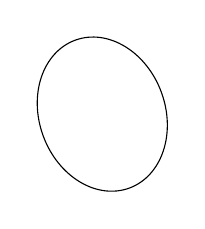
\begin{tikzpicture}[x=1mm, y=1mm]
\draw[rotate=20] (0,0) ellipse (8mm and 10mm);
\end{tikzpicture}}}\par\smallskip}
\end{GelfandAdjacentEvidence}

$U$ — a circle, $U$ — also a circle, a map of degree 2
$U\to U$.



\begin{GelfandAdjacentEvidence}{GELFAND-P000230}{6}
\begin{equation*}
 U\times_U U=U.
\end{equation*}







\SourceFigure{GELFAND-P000230}{degree-two-diamond}{\par\smallskip\centering{\color{black}\GelfandFitDiagram{
\begin{tikzpicture}[x=1mm, y=1mm,>=stealth]
\node at (20,30) {$U$};
\node at (0,13) {$U$};
\node at (40,13) {$U$};
\node at (20,-6) {$U$};
\draw[->] (14,26)--(5,18);
\draw[->] (26,26)--(35,18);
\draw[->] (5,7)--(14,-1);
\draw[->] (35,7)--(26,-1);
\end{tikzpicture}
}}\par\smallskip}
\end{GelfandAdjacentEvidence}
\begin{GelfandAdjacentEvidence}{GELFAND-P000230}{7}

$U_1\times_X U_2$ —
\Unclear{GELFAND-P000230}{join-operations}{перемн. и склеив. / пересеч. и склеив. (multipl. and gluing / intersect. and gluing); the first abbreviation is not uniquely established.}
\end{GelfandAdjacentEvidence}

— a disconnected union.

2 and 3 sheets $\Rightarrow$ 6 sheets



\begin{gather*}
 \mathbb Z_2\times\mathbb Z_2\ne\mathbb Z_4,\\
 \mathbb Z_2\times\mathbb Z_3=\mathbb Z_6.
\end{gather*}





\SourcePage{GELFAND-P000231}{unlabelled}
Presheaf: $\bullet$ a functor



\begin{gather*}
 \operatorname{Cat}T\to\mathrm{Ab}\qquad\text{(contravar.)}\\
 u\to P (u)
\end{gather*}



\begin{equation*}
 v\to u\;\Rightarrow\; P (u)\to P (v)
\end{equation*}



\begin{GelfandAdjacentEvidence}{GELFAND-P000231}{0}
A sheaf — a presheaf satisfying the axioms:



1. $\xi\in P (u)$

$\{u_i\to u\}$ — a covering
\begin{equation*}
 \xi\to\xi_i\qquad P (u)\to P (u_i)
\end{equation*}
$\xi$ is uniquely determined by $\xi_i$




\end{GelfandAdjacentEvidence}
\begin{GelfandAdjacentEvidence}{GELFAND-P000231}{1}
2. and is indeed determined, if $\xi_i$ agree on intersections







\SourceFigure{GELFAND-P000231}{framed-intersection}{\par\smallskip\centering{\color{black}\GelfandFitDiagram{
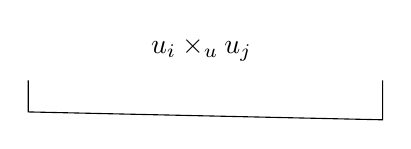
\begin{tikzpicture}[x=1mm, y=1mm]
\node at (22,5) {$u_i\times_u u_j$};
\draw (0,1)--(0,-3)--(45,-4)--(45,1);
\end{tikzpicture}
}}\par\smallskip}
\end{GelfandAdjacentEvidence}

Define Čech cohomology



\begin{align*}
 C^0&=P (u)\\
 C^1&=\prod P (u_i)\\
 C^2&=\prod P (u_i\times_u u_j).\\
 C^3&=\prod P (u_i\times_u u_j\times_u u_k)
\end{align*}



$d$ is defined naturally



$\mathcal F\to\Gamma (X,\mathcal F)$ — a functor.



\begin{GelfandAdjacentEvidence}{GELFAND-P000231}{2}
\begin{center}
\begin{tabular}{l}
($\Gamma$ — an abelian group —\\
\hspace{12mm}— a sheaf of groups)
\end{tabular}
\end{center}
\Unclear{GELFAND-P000231}{gamma-gloss}{Both lines of the parenthesis are retained. No separate symbol is visible before the dash in the second line; its implied subject is undetermined.}
\end{GelfandAdjacentEvidence}

\begin{equation*}
 0\to\mathcal F_1\to\mathcal F_2\to\mathcal F_3\to0.
\end{equation*}



— an \underline{exact sequence of sheaves.}



\begin{equation*}
 0\to\Gamma (\mathcal F_1)\to\Gamma (\mathcal F_2)\to\Gamma (\mathcal F_3)
\end{equation*}



(left exact).



\begin{GelfandAdjacentEvidence}{GELFAND-P000231}{91}
Derived functors exist. $R^i: S\to\mathrm{Ab}$



$S$ — arbit. sheaves (category).



\begin{equation*}
 \to R^1(\mathcal F_1)\to\ldots\to R^2(\mathcal F_2)
\end{equation*}



($R^i$ — determined uniquely).
\begin{equation*}
 R^i (\mathcal F)\underset{\mathrm{def}}{=}H^i (X,\mathcal F).
\end{equation*}




\end{GelfandAdjacentEvidence}\begin{GelfandAdjacentEvidence}{GELFAND-P000231}{3}
\underline{Finite group.} Grothendieck top. from representations.







\SourceFigure{GELFAND-P000231}{source-icon}{Separate icon on the source image.\par\smallskip\centering{\color{black}\GelfandFitDiagram{

\begin{tikzpicture}[x=1mm, y=1mm, line width=0.6pt]
\path[draw=black,fill=yellow] (3,3)--(8,3)--(7,0)--(11,3)--(22,3)
 .. controls (25,3) and (26,5) .. (26,8)--(26,17)
 .. controls (26,20) and (24,22) .. (21,22)--(4,22)
 .. controls (1,22) and (0,20) .. (0,17)--(0,8)
 .. controls (0,5) and (1,3) .. (3,3)--cycle;
\draw (5,17)--(21,17);
\draw (5,12)--(21,12);
\draw (5,7)--(17,7);
\end{tikzpicture}
}}\par\smallskip}
\end{GelfandAdjacentEvidence}



\SourcePage{GELFAND-P000232}{unlabelled}
11/III \underline{Gelfand} (and Kirillov)



$\mathfrak g$ — semisimple Lie algebra, (over $C$)



$U (\mathfrak g)$ — its enveloping algebra



(polyn. in generators $e_1,\ldots, e_n$,
\begin{equation*}
 e_i e_k-e_k e_i=\sum C^j_{ik}e_j
\end{equation*}



$Z (\mathfrak g)$ — centre of the enveloping algebra

(its elements — Laplace or Casimir operators).



Repr. of $G\Rightarrow$ diff. operators and commut.



\begin{GelfandAdjacentEvidence}{GELFAND-P000232}{1}
$Z (\mathfrak g)$ — commut. with the action of the \Unclear{GELFAND-P000232}{centre-end}{group}
\end{GelfandAdjacentEvidence}


Such a repr. of the enveloping alg. by diff. operators is not necessarily faithful.



On $G$ itself — faithful (transform.)



For $Z (\mathfrak g)$ it makes no difference, left or right.



$\mathfrak g$ — semisimple Lie algebra. (over $C$).



\begin{GelfandAdjacentEvidence}{GELFAND-P000232}{2}
$N_-$ — $\max$ nilpot. \Unclear{GELFAND-P000232}{nilpotent-corrections}{[crossed out: group algebra] [inserted below the first word: group]}
\end{GelfandAdjacentEvidence}
\begin{GelfandAdjacentEvidence}{GELFAND-P000232}{3}
 (triang. matr.)

\Unclear{GELFAND-P000232}{quotient-correction}{$N_-\backslash G$ [upper right symbol heavily overwritten]}
\end{GelfandAdjacentEvidence}


\begin{GelfandAdjacentEvidence}{GELFAND-P000232}{4}
\underline{Theorem:} in $N_-\backslash G$ the repr. of $U (\mathfrak g)$ is faithful.



\Unclear{GELFAND-P000232}{theorem-adjective}{(simple).}
\end{GelfandAdjacentEvidence}


$f$ on the group is regular if its translates — finite-dim. space

($\sin$ on the line)



On a comp. group, functions are approx. by regular ones (completeness theorem)



Consider functions $f (g)\equiv f (n_-g)$ — invar. — ring.



Consider $\operatorname{Spec}$ of this ring. This is $X$.



$N_-\backslash G$ birat. equiv. to projective space.



Enveloping algebras are numerous, but division rings, of fractions are few



\begin{equation*}
 \underset{\substack{\text{division ring}\\\text{of quotients}}}{D (\mathfrak g)}\sim D_{n, k}
\end{equation*}



Nontriv. that embeds into a division ring (!) of quotients.



\begin{GelfandAdjacentEvidence}{GELFAND-P000232}{5}
\begin{equation*}
 x_1,\ldots, x_n;\quad
 \frac{\partial}{\partial x_1},\ldots,\frac{\partial}{\partial x_n},\quad
 y_1,\ldots, y_k
\end{equation*}



\Unclear{GELFAND-P000232}{operator-letter}{$\ell (x,\frac{\partial}{\partial x}, y)$}
\end{GelfandAdjacentEvidence}


$\underline{\underline{QP^{-1}}}\; Q_1P_1^{-1}$ and so on. Everything can be done in 2 steps.

($QP^{-1}$ suffices)



$n$ — number of variables, $k$ — number of parameters — invariants.





\begin{GelfandAdjacentEvidence}{GELFAND-P000233}{1}
\SourcePage{GELFAND-P000233}{23}




\SourceFigure{GELFAND-P000233}{source-number}{\par\smallskip\centering{\color{black}\GelfandFitDiagram{
\begin{tikzpicture}[x=1mm, y=1mm]
\node at (9,6) {$23$};
\draw (0,14)--(0,0)--(18,0);
\end{tikzpicture}
}}\par\smallskip}
\end{GelfandAdjacentEvidence}\begin{GelfandAdjacentEvidence}{GELFAND-P000233}{91}


For a semisimple group it is almost proved that $D (\mathfrak g)\sim D_{n, k}$.




(\Unclear{GELFAND-P000233}{top-parenthesis}{постр.}

 is valid)

\end{GelfandAdjacentEvidence}

\begin{GelfandAdjacentEvidence}{GELFAND-P000233}{3}
For nilpotent proved, and probably for algebraic solvable.




\SourceFigure{GELFAND-P000233}{central-extension}{\par\smallskip\centering{\color{black}\GelfandFitDiagram{\begin{minipage}{68mm}\raggedright 
Adjoin to $Z (\mathfrak g)$ \tikz[baseline=(k.base)]{\node[draw, circle, inner sep=1pt] (k) {$K$};} operators — virtual Laplace operators
\end{minipage}}}\par\smallskip}
\end{GelfandAdjacentEvidence}
\begin{GelfandAdjacentEvidence}{GELFAND-P000233}{4}

New ring $\tilde U (\mathfrak g)$ — with adjoined left translations



\Incomplete{GELFAND-P000233}{crossed-top}{A short word or abbreviation is crossed out; its letters beneath the heavy strokes have not been established.}
\end{GelfandAdjacentEvidence}

\begin{equation*}
 U (\mathfrak g)\otimes_{Z (\mathfrak g)}\tilde Z (\mathfrak g)=\tilde U (\mathfrak g).
\end{equation*}



$\tilde Z$ — $Z$ with adjoined virt. Laplace operators.



(this is an algebraic extens., Galois group — Weyl group).



\underline{Theorem.} The division ring of fractions of $\tilde U (\mathfrak g)$ is $D_{n, k}$.



(For $U$ unknown; done for unimodular).



Alg. extens. of $D_{n, k}$ — ?.



\begin{GelfandAdjacentEvidence}{GELFAND-P000233}{5}
In the commut. case, alg. varieties.




\SourceFigure{GELFAND-P000233}{question}{\par\smallskip\centering{\color{black}\GelfandFitDiagram{\begin{minipage}{68mm}\raggedright 
\underline{Question.} There are compact 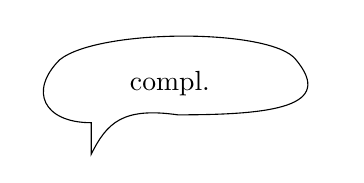
\begin{tikzpicture}[x=1mm, y=1mm, baseline=(c.base)]
\node[inner sep=1pt] (c) at (15,5) {compl.};
\draw (1,8).. controls (6,12) and (28,12) .. (31,8)
 .. controls (36,2) and (28,1) .. (16,1)
 .. controls (9,2) and (7,0) .. (5,-4)
 --(5,0).. controls (-1,0) and (-3,4) .. (1,8);
\end{tikzpicture} manif.

Describe regular differential operators
\end{minipage}}}\par\smallskip}
\end{GelfandAdjacentEvidence}

On the Riemann sphere $\frac{\partial}{\partial z},\; z\frac{\partial}{\partial z},\; z^2\frac{\partial}{\partial z}$



\underline{On Dixmier's work} (Limanov).



\begin{GelfandAdjacentEvidence}{GELFAND-P000233}{6}
$R_{1,0}$ — ring of quantum mech. — generators $x,\frac{d}{dx}$.







\SourceFigure{GELFAND-P000233}{polynomial-callout}{\par\smallskip\centering{\color{black}\GelfandFitDiagram{
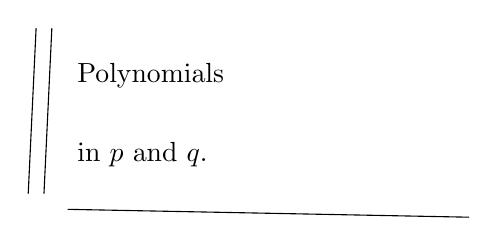
\begin{tikzpicture}[x=1mm, y=1mm]
\node[anchor=west] at (5,15) {Polynomials};
\node[anchor=west] at (5,5) {in $p$ and $q$.};
\draw (0,0)--(1,21);
\draw (2,0)--(3,21);
\draw (5,-2)--(56,-3);
\end{tikzpicture}
}}\par\smallskip}
\end{GelfandAdjacentEvidence}

$p, q,\quad [p, q]=1$.



\begin{GelfandAdjacentEvidence}{GELFAND-P000233}{7}
The autom. group is generated by triang. autom.



\Unclear{GELFAND-P000233}{first-shear}{$\left\{\begin{aligned}p&\to p\\q&\to q+f (p)\end{aligned}\right. $}
\end{GelfandAdjacentEvidence}

and
$\left\{\begin{aligned}p&\to p+g (q)\\q&\to q\end{aligned}\right. $



For the division ring $D_{1,0}$ unknown.



\begin{GelfandAdjacentEvidence}{GELFAND-P000233}{8}
Or \Unclear{GELFAND-P000233}{bottom-cancellation}{[crossed-out symbol: и? от?]}
\end{GelfandAdjacentEvidence}


$\left\{\begin{aligned}q&\to q\\p&\to p+g (q)\end{aligned}\right. $



and
$\left\{\begin{aligned}q&\to p\\p&\to -q\end{aligned}\right. $

(Fourier transform)



Is generated





\SourcePage{GELFAND-P000234}{unlabelled}
Arnold: theor.



\begin{GelfandAdjacentEvidence}{GELFAND-P000234}{1}
Let there be functions $f (p, q)$



\Unclear{GELFAND-P000234}{poisson-index}{$[f_1(p, q), f_2(p, q)]=\dfrac{\partial f_1}{\partial p}\cdot\dfrac{\partial f_2}{\partial q}-\dfrac{\partial f_1}{\partial q}\cdot\dfrac{\partial f_2}{\partial p}$. [Index in the first factor after the minus: $1$ or $2$.]}
\end{GelfandAdjacentEvidence}

Consider 2 polynomials
\begin{gather*}
 P=P (p, q)\\
 Q=Q (p, q).
\end{gather*}



Substitute $P$ and $Q$ — will be 1.



They induce canon. transformations of quasiclassics.



But there is no connection, even with grading.



An element $x$ is completely semisimple if the transformation $\operatorname{ad}X$ has a complete system of eigenvalues.



\begin{GelfandAdjacentEvidence}{GELFAND-P000234}{2}
Then by an automorph. $x$ is carried into $x\to pq$.




\SourceFigure{GELFAND-P000234}{euler}{\par\smallskip\centering{\color{black}\GelfandFitDiagram{\begin{minipage}{68mm}\raggedright 
\begin{tikzpicture}[x=1mm, y=1mm, baseline=(e.base)]
\node[inner sep=0pt] (e) at (11,7) {$x\dfrac{d}{dx}$};
\draw (-2,3)--(-2,0)--(24,0)--(24,3);
\end{tikzpicture} — eigenfunctions — homog. polynomials.
\end{minipage}}}\par\smallskip}
\end{GelfandAdjacentEvidence}

\begin{equation*}
 p^a q^b\to (a-b)p^a q^b.
\end{equation*}



\begin{GelfandAdjacentEvidence}{GELFAND-P000234}{3}
Result of \Unclear{GELFAND-P000234}{amitsur-name}{Амицури or Амицура}

:

$x$\qquad $C (x)$ — commuting — commut. subalgebra.
\end{GelfandAdjacentEvidence}



But these are not always polynomials.



\begin{equation*}
 \forall\alpha\ \exists X, Y,\qquad X^3=Y^2+\alpha,\qquad \alpha\in C.
\end{equation*}



\underline{Palamodov.}



on Hörmander's work (on $\bar\partial$)



2 main results: existence theorem and approx. theorem.



1. $\Omega\subset C^n$, $\phi\in C^2(\Omega)$
\begin{equation*}
 L (\phi)=\frac{\partial^2\phi}{\partial z_j\partial\bar z_k}\xi_j\bar\xi_k\ge0
\end{equation*}



\begin{equation*}
 L_{p, q}=L_{p, q}(\Omega,\phi),\qquad
 \|f\|_\phi^2=\int_\Omega |f|^2e^{-\phi}dV
\end{equation*}
forms of type $(p, q)$



\begin{GelfandAdjacentEvidence}{GELFAND-P000234}{4}
Let $\phi$ be plurisubh. in $\Omega$ \Unclear{GELFAND-P000234}{plurisub-correction}{[overlapping strokes before the parenthesis]}
\end{GelfandAdjacentEvidence}
 (therefore real) and

$\forall c\ \{\phi\le c\}$ — compact. ($\Rightarrow\Omega$ — pseudoconvex)



Then $\forall f\in L_{p, q}$, $\bar\partial f=0$



\begin{GelfandAdjacentEvidence}{GELFAND-P000234}{5}
$\exists$ \Incomplete{GELFAND-P000234}{cancelled-existence}{Crossed-out fragment; its initial symbol resembles $g$, the remaining letters have not been established.}
\end{GelfandAdjacentEvidence}

$g$ of type $p, q-1$



\begin{equation*}
 \bar\partial g=f\qquad\overset{(q\ge1)}{\text{and}}\qquad
 g\in L_{p, q-1}(\Omega,\phi+2\ln (1+|z|^2))
\end{equation*}



Here $\sqrt q\,\|g\|\le\|f\|$ (assuming $q\ge1$)





\begin{GelfandAdjacentEvidence}{GELFAND-P000235}{1}
\SourcePage{GELFAND-P000235}{24}



\SourceFigure{GELFAND-P000235}{source-number}{\par\smallskip\centering{\color{black}\GelfandFitDiagram{\begin{tikzpicture}[x=1mm, y=1mm]
\node at (9,6) {$24$};\draw (0,14)--(0,0)--(18,0);
\end{tikzpicture}}}\par\smallskip}
\end{GelfandAdjacentEvidence}

\begin{GelfandAdjacentEvidence}{GELFAND-P000235}{2}
2. \underline{Approx. theorem.}

$\Omega=C^n$.



\Unclear{GELFAND-P000235}{revised-weight}{The former second argument is crossed out: $\phi$ or $\psi$; $\phi+c\ln (1+|z|^2)$ is inserted below. \par\smallskip\centering{\color{black}\GelfandFitDiagram{\begin{tikzpicture}[x=1mm, y=1mm]
\node[anchor=west, font=\small] at (0,10) {$f\in L_{0,0}(\Omega, [?])$};
\node[anchor=west, font=\small] at (20,-3) {$\phi+c\ln (1+|z|^2)$};
\node[anchor=west, font=\small] at (47,10) {$\bar\partial f=0$};
\node[anchor=west, font=\small] at (75,10) {(holom. functions)};
\draw (44,18)--(44,3)--(73,0)--(73,-8)--(65,-8);
\end{tikzpicture}}}\par\smallskip}
\end{GelfandAdjacentEvidence}




i.e. $|f|\le Ce^\phi (1+|z|^2)^k$, ($\exists C>0$).



This set is nonempty (nontriv. — $\Omega=C^n$). — and dense in the space of all $\underset{\text{entire}}{\text{[holom.]}}$ functions with unif. convergence on $\forall$ compact set:



$\phi$ — homog. along radii $\Rightarrow$ indicator of an entire function.



\begin{GelfandAdjacentEvidence}{GELFAND-P000235}{3}
Hence \underline{Martino}: the class of indicators — all radially homog. plurisubh. harm.



\Unclear{GELFAND-P000235}{indicator-limit}{\par\smallskip\centering{\color{black}\GelfandFitDiagram{\begin{tikzpicture}[x=1mm, y=1mm]
\node at (0,0) {$i (z)=$};
\node at (23,0) {$\displaystyle\lim_{\tau\to\infty}$};
\node at (68,0) {$\tau^{-k}\ln|f (z\tau)|$};
\draw (13,12)--(13,8)--(38,8);
\draw (38,8)--(100,8)--(100,-7)--(38,-7)--cycle;
\end{tikzpicture}}}\par\smallskip The affiliation of the stroke above $\lim$ has not been established.}
\end{GelfandAdjacentEvidence}

18/III



If $\phi=\phi (x)$ (only on the real parts), it is plurisubharm. if and only if it is convex.



In $\forall$ one-dim. complex space subharm.



\underline{Example:}
\begin{equation*}
 \frac{\partial u}{\partial\bar z}=f,\qquad
 |f (z)|\le Ce^{a|\operatorname{Im}z|}(1+|z|^2)^k.
\end{equation*}



A solution in this class — nontrivial.



\begin{GelfandAdjacentEvidence}{GELFAND-P000235}{4}
For bounded functions in the unit disk, the equation \Unclear{GELFAND-P000235}{disk-derivative}{$\dfrac{\partial u}{\partial z}=f$ [denominator: $z$ or $\bar z$]}
\end{GelfandAdjacentEvidence}
 is not necessarily solvable
for bounded $f$.



For solvability it suffices



\begin{GelfandAdjacentEvidence}{GELFAND-P000235}{5}
($f$ — measure)



\Unclear{GELFAND-P000235}{disk-figure}{\par\smallskip\centering{\color{black}\GelfandFitDiagram{\begin{tikzpicture}[x=1mm, y=1mm, line width=0.6pt]
\draw (0,0) ellipse [x radius=13,y radius=12];
\draw[white,line width=1.2pt] (-11,6).. controls (-8,12) and (-3,13) .. (4,11.4);
\draw[gray,line width=0.35pt] (-11,6).. controls (-9,10) and (-7,11) .. (-5,11.4);
\draw[gray,line width=0.35pt] (-3,12.2)--(-1.5,12.3);
\draw (6,10) ellipse [x radius=6,y radius=5];
\path[fill=black] (-1,-1) circle [radius=0.6];
\draw[line width=1pt] (1,11).. controls (3,13) and (5,13) .. (7,11);
\draw (3,8)--(6,11)--(12,5);
\draw (6,11)--(6,8.7);
\node at (15,16) {$S$};
\end{tikzpicture}}}\par\smallskip The faint upper arc and dark strokes at the intersection are transcribed without an established meaning for the strokes.}
\end{GelfandAdjacentEvidence}

$S$ — disk. $|f (S\cap\Omega)|\le C R_S$.



\begin{GelfandAdjacentEvidence}{GELFAND-P000235}{91}
\underline{Theorem 3.} More precise theorem for fixed $q$.



Let $\partial\Omega\in C^3$ and the domain be bounded. Local condition on the boundary:



$\forall z\in\partial\Omega\ \exists\phi\in C^2$ such that $\Omega=\{\phi (z)<\phi (z_0)\}$ in a nbhd. of this point.



Condition $a_q$:
\begin{equation*}
 \sum\frac{\partial^2\phi}{\partial z_j\partial\bar z_k}\xi_j\bar\xi_k
 \quad\text{on}\quad
 \sum\frac{\partial\phi}{\partial z_j}\xi_j=0
\end{equation*}



has —
\begin{equation*}
 \left\{\begin{aligned}&q+1\ \text{negative}\\&\text{or }n-q\ \text{positive}\end{aligned}\right.
 \quad\Vert\quad\substack{\text{eigen-}\\\text{values}}
\end{equation*}




\end{GelfandAdjacentEvidence}\underline{Gelfand:} domains of regularity — ?



Palam. says nobody is working on this.



$\partial\Omega$ pseudoconvex if at $\forall$ point condition $a_0$ (at $\forall$ point $n-1$ positive eigenvalues)



In the tangent space, $n-q$-dim. surfaces along which the domain is pseudoconvex.



Let $a_q$ hold at $\forall$ boundary point.



\begin{equation*}
 L_{p, q-1}\overset{\bar\partial}{\longrightarrow}
 L_{p, q}(\Omega,\phi)\overset{\bar\partial}{\longrightarrow}L_{p, q+1}
\end{equation*}



\begin{GelfandAdjacentEvidence}{GELFAND-P000235}{6}
Cohomology \Unclear{GELFAND-P000235}{cancelled-cohomology-word}{[crossed out below: kernel, ядро or ядра]}

is finite-dimensional and the image is closed.
\end{GelfandAdjacentEvidence}
\begin{GelfandAdjacentEvidence}{GELFAND-P000235}{7}
 



\Unclear{GELFAND-P000235}{isolated-mark}{\par\smallskip\centering{\color{black}\GelfandFitDiagram{\begin{tikzpicture}[x=1mm, y=1mm]
\draw (2,16).. controls (-1,12) and (-1,4) .. (2,1);
\draw (0,13)--(10,13);
\draw (0,8)--(9,8);
\draw (3,4)--(10,4)--(10,9);
\end{tikzpicture}}}\par\smallskip Isolated sign: $E$ or $\exists$; its function has not been established.}
\end{GelfandAdjacentEvidence}

Existence of a function $\Psi$ on the whole domain.



\begin{GelfandAdjacentEvidence}{GELFAND-P000235}{8}
$\Psi$ — real, defined inside $\Omega$,



\Unclear{GELFAND-P000235}{last-hessian-index}{$\dfrac{\partial^2\Psi}{\partial z_i\partial\bar z_k}\eta_j\bar\eta_k$ [first denominator index: $i$ or $j$]}
\end{GelfandAdjacentEvidence}

satisfies all conditions



(1 more plus required, since in the whole space)



Then cohomology 0.





\begin{GelfandAdjacentEvidence}{GELFAND-P000236}{91}
\SourcePage{GELFAND-P000236}{unlabelled}
All these theorems for complex spaces — Andreotti and Grauert.



1. Runge-type theorem.



$\omega\subset\Omega$, $L (\Psi)$ at $\forall$ point of $\Omega\setminus\omega$ satisfies the condition



\begin{gather*}
 q+1\quad -\\
 \text{or}\\
 n-q+1\quad +
\end{gather*}



$\Psi\to\infty$ near $\partial\Omega$, $\{\Psi<0\}=\omega$



Then the cohomology of $\Omega$ restricts monomorphically to the cohom. of $\omega$.



A closed form $f$ in $\Omega$ and the equation $\bar\partial u=f$ solvable in $\omega\Rightarrow$ it is solvable in $\Omega$ as well.



2. Approximation theorem.



Closed forms in $\omega$ are approximated by closed forms in $\Omega$.




\end{GelfandAdjacentEvidence}\begin{GelfandAdjacentEvidence}{GELFAND-P000236}{1}
\underline{Existence theorem.}

Let $\partial\Omega\in C^2$ and there exist $\rho$, $\{\rho<0\}=\Omega$,






\SourceFigure{GELFAND-P000236}{boundary-conditions}{\par\smallskip\centering{\color{black}\GelfandFitDiagram{\begin{tikzpicture}[x=1mm, y=1mm]
\node[anchor=west] at (6,24) {$\operatorname{grad}\rho|_{\partial\Omega}\ne0, $};
\node[anchor=west] at (6,14) {$\dfrac{\partial^2\rho}{\partial z_j\partial\bar z_k}\xi_j\bar\xi_k\ge0$};
\node[anchor=west] at (27,3) {when $\displaystyle\sum\frac{\partial\rho}{\partial z_j}\xi_j=0.$};
\draw (0,29)--(0,-3).. controls (16,-4) and (31,-6) .. (44,-7);
\draw (1.5,29)--(1.5,-2);
\draw (57,-8)--(102,-9);
\end{tikzpicture}}}\par\smallskip}
\end{GelfandAdjacentEvidence}\begin{GelfandAdjacentEvidence}{GELFAND-P000236}{92}


It is proved simply, using the identity.



\begin{equation*}
 L_{p, q-1}\overset{\bar\partial=T}{\longrightarrow}L_{p, q}
 \overset{\bar\partial=S}{\longrightarrow}L_{p, q+1}
\end{equation*}



\begin{equation*}
 \|T^*f\|_\phi^2+\|Sf\|_\phi^2=
\end{equation*}



\begin{equation*}
 (u, v)_\phi=\int_\Omega u\bar v e^{-\phi}dV.
\end{equation*}



(adjoint with respect to this inner product)



\begin{equation*}
 =\sum_L\sum_{j, k}\left (\frac{\partial^2\phi}{\partial z_j\partial\bar z_k}f_{jL}, f_{kL}\right)_\phi
 +\sum_J\sum_k\left\|\frac{\partial f_J}{\partial\bar z_k}\right\|_\phi^2+
\end{equation*}




Take $p=0$ (for simplicity — expansion in \Unclear{GELFAND-P000236}{assume-p-zero}{$dz$ [first symbol heavily overwritten; reading not established]}

).

\begin{equation*}
 f=\sum f_Jd\bar z^J,\qquad J=j_1,\ldots, j_q.
\end{equation*}



$f_J$ skew-symm. in the indices, $jL$ — long index.



\begin{equation*}
 +\sum\sum\int_{\partial\Omega}\frac{\partial^2\rho}{\partial z_j\partial\bar z_k}f_{jL}\overline{f_{kL}}e^{-\phi}dS.
\end{equation*}



The identity — integration by parts.



First — Morri with $\phi=0$.



$\operatorname{grad},\operatorname{rot}$ — known in mechanics.



Solvability follows from it.



Next time — Nirenberg (according to hearsay).




\end{GelfandAdjacentEvidence}


\clearpage\section*{Chapter 4}

\Needspace{7\baselineskip}
\begin{GelfandAdjacentEvidence}{GELFAND-P000237}{1}
\SourcePage{GELFAND-P000237}{unlabelled}
\Unclear{GELFAND-P000237}{top-right-label}{[At the upper right: $1$ / $l$.]}
\end{GelfandAdjacentEvidence}

\underline{Seminar} \quad \underline{of Gelfand.} \quad 1968-69.



\begin{GelfandAdjacentEvidence}{GELFAND-P000237}{2}
1. Mumford. Moduli spaces. (Geronimus Sasha)



\Unclear{GELFAND-P000237}{list-two-cancelled}{2. [Cancelled: Kr.]}
\end{GelfandAdjacentEvidence}

Kirillov. Characters. (lectures)



3. Kazhdan \quad Dwork ?



4. Griffiths \quad Mixture of diff. eqs., geom., top., complex analysis



5. Spencer resolution. (Palamodov)



6. \textbf{Gromov}

\textbf{7.} \textbf{Buslaev} on eigenvalues (incl. Maslov's work)



8. Grauert and Remmert, $\boldsymbol{p}$-adic analysis.

(old idea of L. G. Shnirelman about the Cauchy $\int$ and the like over an arbitrary field)



\textbf{9. Nilson}



\begin{GelfandAdjacentEvidence}{GELFAND-P000237}{3}
\textbf{10.} Vershik on factors $\underline{\overline{\mathrm{II}}}$ and $\underline{\overline{\mathrm{III}}}$



\Unclear{GELFAND-P000237}{sinai-superscript}{or Sinai (and $K^0$ / $K^{\circ}$)}
\end{GelfandAdjacentEvidence}

11. H\"ormander \quad work on Lie groups and diff. eqs. (hypoell.).



Idea of \textbf{Dwork} (Kazhdan)



If some series converges near $0$ in a complex variable and at every $p$-adic one, then it is a rational function.



idea: represent the $\zeta$-function using ([Above the line: in] $p$-adic variables) completely continuous operators.



[Wavy underlining: On Gromov:] 2 extreme cases which are unified.



Bundle techniques are transferred to foliations (sometimes). For foliations of dimension $1$ — the question of a vector field.



[Wavy underlining on two lines:]
A foliation of codim. $\geq1$ always exists if a family of planes exists (!)



The sheaf of germs and jets — a weak homotopy equiv.



\begin{GelfandAdjacentEvidence}{GELFAND-P000237}{4}
(If there is a set of \underline{coeff.} \underline{glob.}, then one can construct a function)



\Unclear{GELFAND-P000237}{psychology-college}{\underline{Psych. experiment} \quad \underline{in an Eng. / Am. coll.}}
\end{GelfandAdjacentEvidence}

Tests $\Rightarrow$ teachers secretly told about the giftedness of $20\%$ of the pupils, selected by lot $\Rightarrow$ after a year they are $1.5$ times better than avg.! (not by marks, but by tests)





\Needspace{7\baselineskip}
\SourcePage{GELFAND-P000238}{unlabelled}
\underline{\underline{Geronimus}} on Mumford.



[Wavy underlining: Object of study] — compact Riem. surfaces.



$\underline{g=0}$ — all isomorphic (sphere).



\begin{GelfandAdjacentEvidence}{GELFAND-P000238}{1}
$\underline{\underline{g=1}}$ — complex elliptic curves.




\SourceFigure{GELFAND-P000238}{universal-cover}{\par\smallskip\centering{\color{black}\GelfandFitDiagram{\begin{minipage}{68mm}\raggedright 
$X$ — surface of genus $1$.
\begin{center}\GelfandFitDiagram{\begin{tikzpicture}[x=1mm, y=1mm]
\node at (0,15) {$\overline X$};\node at (0,0) {$X$};
\draw[->] (0,11)--(0,4);
\end{tikzpicture}}\end{center}
— universal cover. It is the plane (analytically)
\end{minipage}}}\par\smallskip}
\end{GelfandAdjacentEvidence}

$Z+Z$ acts without fixed points
\begin{equation*}z\to z+b\qquad (b_1, b_2)\end{equation*}



\begin{GelfandAdjacentEvidence}{GELFAND-P000238}{2}
\underline{When} do we obtain different surfaces?



\Unclear{GELFAND-P000238}{elliptic-comparison}{\par\smallskip\centering{\color{black}\GelfandFitDiagram{\begin{tikzpicture}[x=1mm, y=1mm]
\node at (0,20) {$X$};\node at (27,20) {$X'$};
\node at (0,0) {$X$};\node at (27,0) {$X'$};
\draw (-3,26)--(3,26);\draw (24,26)--(30,26);
\draw[->] (5,20)--(22,20);\node at (13.5,27) {$lz+m$};
\draw[->] (0,15)--(0,5);
\draw[->] (5,0)--(22,0);\node at (13.5,5) {$\sim$};
\end{tikzpicture}}}\par\smallskip
[The attachment of the rules above the upper letters is not established.]}
\end{GelfandAdjacentEvidence}
\begin{GelfandAdjacentEvidence}{GELFAND-P000238}{3}

\Unclear{GELFAND-P000238}{lattice-second-index}{\begin{equation*}
\begin{cases}b_1=l b'_1,\\b_2=l b'_i.\end{cases}
\end{equation*}
[Final index in the second line: $i$ / $2$.]}
\end{GelfandAdjacentEvidence}

One can assume ($b_i\ne0$) that $b_1=1$.



$(1, z_2)$ \quad an automorphism of $Z+Z$ also changes nothing.



\begin{GelfandAdjacentEvidence}{GELFAND-P000238}{4}
\begin{equation*}(1, z)\qquad\operatorname{Im}z>0\end{equation*}
\begin{equation*}\operatorname{SL}(2, Z)=\Gamma\end{equation*}



\Unclear{GELFAND-P000238}{fractional-linear-formula}{\begin{equation*}
z_2=\frac{d z_1+b}{c z_1+b}\qquad\begin{pmatrix}a&b\\c&d\end{pmatrix}\in\Gamma
\end{equation*}
[First numerator coefficient: $d$ / $a$; last denominator coefficient: $b$ / $d$.]}
\end{GelfandAdjacentEvidence}
\begin{GelfandAdjacentEvidence}{GELFAND-P000238}{5}


\SourceFigure{GELFAND-P000238}{quotient-action}{\par\smallskip\centering{\color{black}\GelfandFitDiagram{\begin{minipage}{68mm}\raggedright 
Thus, the quotient of the upper half-plane $H$ by
\begin{center}\GelfandFitDiagram{\begin{tikzpicture}[x=1mm, y=1mm]
\node at (0,7) {the action};
\draw (-12,1).. controls (-31,1) and (-29,15) .. (-12,16)
 .. controls (8,21) and (30,13) .. (25,5)
 .. controls (24,0) and (7,0) .. (-4,1)
 --(-13,-6)--(-12,1);
\end{tikzpicture}}\end{center}
of the unimodular group $\Gamma$
\end{minipage}}}\par\smallskip}
\end{GelfandAdjacentEvidence}

\begin{equation*}H\longrightarrow H/\Gamma=\Pi\end{equation*}



\begin{GelfandAdjacentEvidence}{GELFAND-P000238}{6}
On $H$ there is a fund. domain




\SourceFigure{GELFAND-P000238}{fundamental-domain}{\par\smallskip\centering{\color{black}\GelfandFitDiagram{\begin{minipage}{148mm}\raggedright 
\begin{center}\GelfandFitDiagram{\begin{tikzpicture}[x=18mm, y=12mm]
\draw (-1.7,0)--(1.9,0);
\draw (-1,0).. controls (-.75,.6) and (-.45,.95) ..(0,1)
 .. controls (.55,1.03) and (.8,.65) ..(1,0);
\draw[dashed] (-.45,0)--(-.45,.9);
\draw (.45,0)--(.45,.9);
\draw[line width=.7pt] (-.45,.9)--(-.45,2.7)--(.45,2.85)--(.45,.9);
\draw (-.42,1.03)--(.36,1.19);
\draw (-.37,1.23)--(.34,1.44);
\draw (-.38,1.48)--(.35,1.61);
\draw (-.22,1.67)--(.35,1.86);
\draw (-.39,1.90)--(.37,2.08);
\draw (-.37,2.12)--(.38,2.32);
\draw (-.40,2.34)--(.38,2.53);
\draw (-.38,2.53)--(.37,2.70);
\node[below] at (-1,0) {$-1$};\node[below] at (-.45,0) {$-\frac12$};
\node[below] at (.45,0) {$\frac12$};\node[below] at (1,0) {$1$};
\node[anchor=west, align=left] at (2.2,1.7) {this is a fund.\\domain};
\end{tikzpicture}}\end{center}
\end{minipage}}}\par\smallskip}
\end{GelfandAdjacentEvidence}

The plane — the analytic manifold of all elliptic curves.



\begin{GelfandAdjacentEvidence}{GELFAND-P000238}{7}
\underline{\underline{General def. 1}}



There is a collection of analytic manifolds $K$.




\SourceFigure{GELFAND-P000238}{moduli-family}{\par\smallskip\centering{\color{black}\GelfandFitDiagram{\begin{minipage}{68mm}\raggedright 
Moduli space — an analytic manifold with a map
\begin{center}\GelfandFitDiagram{\begin{tikzpicture}[x=1mm, y=1mm]
\node at (0,17) {$X$};\node at (0,0) {$\underline Y$};
\draw[->] (0,12)--(0,5);\node at (6,8) {$p$};
\end{tikzpicture}}\end{center}
\end{minipage}}}\par\smallskip}
\end{GelfandAdjacentEvidence}

($X,\underline Y$ — manifolds and an analytic map). Points of $\underline Y$ in one-to-one corresp. with $K$ \begin{tikzpicture}[x=1mm, y=1mm, baseline=0mm]
\draw (0,-2)--(3,7);\draw (1.2,-3)--(4,7);\draw (2.4,-2)--(5,6.5);
\end{tikzpicture}



and, in addition, $p^{-1}(y)\cong$ the corresponding object of $K$



(objects of $K$ cannot be analytically isom.)





\Needspace{7\baselineskip}
\SourcePage{GELFAND-P000239}{2}



$\underline Y=K$ with the structure of an analytic manifold



If the moduli space exists, it is unique up to analytic isom. (easy to prove).



Another def. takes account of possible automorphisms of objects of $K$.



\begin{GelfandAdjacentEvidence}{GELFAND-P000239}{1}
\underline{\underline{Prelim. notion.}}




\SourceFigure{GELFAND-P000239}{family}{\par\smallskip\centering{\color{black}\GelfandFitDiagram{\begin{minipage}{148mm}\raggedright 
\GelfandFitDiagram{\begin{tikzpicture}[x=1mm, y=1mm, baseline=(a.base)]
\node[inner sep=0pt] (a) at (0,0) {Anal.};
\draw (-9,5)--(-9,-4)--(8,-1);\draw (-9,5)--(9,7);
\end{tikzpicture}} \quad \underline{Family of objects of $K$:}
\begin{center}\GelfandFitDiagram{\begin{tikzpicture}[x=1mm, y=1mm]
\node at (0,16) {$X$};\node at (0,0) {$\underline Y$};
\draw[->] (0,11)--(0,5);
\end{tikzpicture}}\end{center}
all fibers isom. to objects of $K$
\end{minipage}}}\par\smallskip}
\end{GelfandAdjacentEvidence}
\begin{GelfandAdjacentEvidence}{GELFAND-P000239}{2}

\begin{tikzpicture}[x=1mm, y=1mm, baseline=(t.base)]
\node[anchor=base west, inner sep=0pt] (t) at (0,0) {Induced family};
\draw[dashed] (t.south west)--(t.south east);
\end{tikzpicture} — analogous to an induced bundle (it always exists)




\SourceFigure{GELFAND-P000239}{pullback-diagram}{\par\smallskip\centering{\color{black}\GelfandFitDiagram{\begin{minipage}{68mm}\raggedright 
\begin{center}\GelfandFitDiagram{\begin{tikzpicture}[x=1mm, y=1mm]
\node at (0,20) {$X''$};\node at (22,20) {$X'$};\node at (52,20) {$X$};
\node at (22,0) {$Y'$};\node at (52,0) {$Y$};
\draw[->] (5,20)--(16,20);\draw[->] (28,20)--(46,20);
\draw[->] (22,15)--(22,5);\draw[->] (52,15)--(52,5);
\draw[->] (28,0)--(46,0);\draw[->] (3,15)--(16,4);
\draw[->] (4,25).. controls (18,33) and (39,31) ..(49,26);
\end{tikzpicture}}\end{center}
\end{minipage}}}\par\smallskip}
\end{GelfandAdjacentEvidence}

This is a commut. diagram $+$ univers.



\begin{GelfandAdjacentEvidence}{GELFAND-P000239}{3}
\begin{tikzpicture}[x=1mm, y=1mm, baseline=(u.base)]
\node[anchor=base west, inner sep=0pt] (u) at (0,0) {Universality};
\draw[dashed] (u.south west)--(u.south east);
\draw[->] (u.east).. controls +(5,0) and +(5,5) ..(u.north east)--(u.north);
\end{tikzpicture}




\SourceFigure{GELFAND-P000239}{universal-projection}{\par\smallskip\centering{\color{black}\GelfandFitDiagram{\begin{minipage}{68mm}\raggedright 
\begin{center}\GelfandFitDiagram{\begin{tikzpicture}[x=1mm, y=1mm]
\node at (0,18) {$X'$};\node at (0,0) {$\underline{Y'}$};
\draw[->] (0,13)--(0,5);\node at (-13,9) {$($};
\node[anchor=west] at (13,9) {univers. $)$};
\end{tikzpicture}}\end{center}
\end{minipage}}}\par\smallskip}
\end{GelfandAdjacentEvidence}
\begin{GelfandAdjacentEvidence}{GELFAND-P000239}{4}


\SourceFigure{GELFAND-P000239}{two-fibers}{\par\smallskip\centering{\color{black}\GelfandFitDiagram{\begin{minipage}{68mm}\raggedright 
\begin{center}\GelfandFitDiagram{\begin{tikzpicture}[x=1mm, y=1mm]
\draw (0,18) ellipse (2.3 and 6);\draw (28,18) ellipse (2 and 6);
\draw (0,0) circle (.6);\draw (28,0) circle (.6);
\end{tikzpicture}}\end{center}
\end{minipage}}}\par\smallskip}
\end{GelfandAdjacentEvidence}
\begin{GelfandAdjacentEvidence}{GELFAND-P000239}{5}

A merely commut. diagram is insufficient (2 points and any one where a map $\exists$).




\SourceFigure{GELFAND-P000239}{product-family}{\par\smallskip\centering{\color{black}\GelfandFitDiagram{\begin{minipage}{68mm}\raggedright 
\begin{center}\GelfandFitDiagram{\begin{tikzpicture}[x=1mm, y=1mm]
\node at (0,19) {$Y'\times X$};\node at (36,19) {$X$};
\node at (0,0) {$Y'$};\node at (36,0) {$\bullet$};
\draw[->] (12,19)--(30,19);\draw[->] (0,14)--(0,5);
\draw[->] (36,14)--(36,4);\draw[->] (6,0)--(31,0);
\end{tikzpicture}}\end{center}
\end{minipage}}}\par\smallskip}
\end{GelfandAdjacentEvidence}

[Wavy underlining: Kirillov] (conjecture)



Representable functor. The representing object is the family of moduli



\begin{GelfandAdjacentEvidence}{GELFAND-P000239}{6}
2 categ. — 1) all analytic spaces.



\Unclear{GELFAND-P000239}{category-cancelled}{functor into the [Cancelled: $2)$ / $2$] category of sets}
\end{GelfandAdjacentEvidence}
\begin{GelfandAdjacentEvidence}{GELFAND-P000239}{7}


\SourceFigure{GELFAND-P000239}{families-functor}{\par\smallskip\centering{\color{black}\GelfandFitDiagram{\begin{minipage}{68mm}\raggedright 
$Y\rightsquigarrow$ set of pairs
\begin{center}\GelfandFitDiagram{\begin{tikzpicture}[x=1mm, y=1mm]
\node at (0,16) {$X$};\node at (0,0) {$\underline Y$};
\draw[->] (0,11)--(0,5);
\end{tikzpicture}}\end{center}
— analytic families.
\end{minipage}}}\par\smallskip}
\end{GelfandAdjacentEvidence}

Repr. of the functor



\begin{equation*}C\overset{F}{\longrightarrow}\mathrm{Ens}\quad (\text{sets})\end{equation*}



\begin{equation*}F_M=\operatorname{Hom}(\bullet, M)\qquad M\text{ — analytic space.}\end{equation*}



\begin{GelfandAdjacentEvidence}{GELFAND-P000239}{8}
\begin{center}\begin{tikzpicture}[x=1mm, y=1mm]
\draw (0,2).. controls (47,6) and (98,-1) ..(150,1);
\draw (0,0).. controls (49,4) and (101,-3) ..(150,0);
\end{tikzpicture}\end{center}




\SourceFigure{GELFAND-P000239}{official-definition}{\par\smallskip\centering{\color{black}\GelfandFitDiagram{\begin{minipage}{148mm}\raggedright 
\begin{center}\GelfandFitDiagram{\begin{tikzpicture}[x=1mm, y=1mm]
\node[align=left] at (-23,12) {Official\\def.};
\draw (-33,20)--(-15,22)--(-15,4)--(-33,4);
\node at (0,20) {$Y$};\node at (0,0) {$S$};
\node at (32,20) {$X$};\node at (32,0) {$M$};
\draw[->] (0,15)--(0,5);\draw[->] (32,15)--(32,5);
\draw[->,dashed] (4,0)--(24,0);
\draw (32,10) ellipse (10 and 17);\draw (32.3,10) ellipse (10.4 and 17.3);
\end{tikzpicture}}\end{center}
— the family is called a moduli manifold if $\forall$ other family is obtained as an induced one.
\end{minipage}}}\par\smallskip}
\end{GelfandAdjacentEvidence}



\Needspace{7\baselineskip}
\SourcePage{GELFAND-P000240}{unlabelled}
A universal family for curves of a given genus does not exist (even for elliptic ones)



Exists for polarized ones (with a chosen homology basis)



\underline{\underline{Modification}} — final object of the category of families



If it does not exist, adjoin it formally.



An additional structure is introduced, allowing cohom. with coeff. in a sheaf to be considered, and so on.



\begin{GelfandAdjacentEvidence}{GELFAND-P000240}{1}
There is no universal object for elliptic curves




\SourceFigure{GELFAND-P000240}{oval-m}{\par\smallskip\centering{\color{black}\GelfandFitDiagram{\begin{minipage}{68mm}\raggedright 
\begin{center}\GelfandFitDiagram{\begin{tikzpicture}[x=1mm, y=1mm]
\draw (0,16).. controls (0,22) and (9,24) ..(9,12)
 .. controls (9,5) and (6,-2) ..(2,0);
\draw[densely dotted] (2,0).. controls (-1,4) and (-1,10) ..(0,16);
\node at (40,-6) {$M$};
\end{tikzpicture}}\end{center}
\end{minipage}}}\par\smallskip}
\end{GelfandAdjacentEvidence}

all points map unambiguously $\Rightarrow$ as a set — elliptic curves do not repeat.



\begin{GelfandAdjacentEvidence}{GELFAND-P000240}{2}
Suppose there is a nontrivial family (base not a point) with identical fibers.
[Above “fibers”: (bundle).]



\Incomplete{GELFAND-P000240}{middle-cancel}{[Cancelled fragment to the right of “fibers”: reading not established.]}
\end{GelfandAdjacentEvidence}
\begin{GelfandAdjacentEvidence}{GELFAND-P000240}{3}

(because there are automorphisms)



\Unclear{GELFAND-P000240}{lower-trivial}{Then the map must be into a point and one obtains triv. / nontriv.}
\end{GelfandAdjacentEvidence}
\begin{GelfandAdjacentEvidence}{GELFAND-P000240}{4}

Exists in a weaker sense — the plane



\Unclear{GELFAND-P000240}{margin-right-sketch}{\par\smallskip\centering{\color{black}\GelfandFitDiagram{\begin{tikzpicture}[x=1mm, y=1mm]
\draw[line width=1pt] (0,25)--(0,0);\draw[line width=1pt] (9,25)--(9,0);
\draw (1,24)--(8,24);\draw (0,0).. controls (3,5) and (6,5) ..(9,0);
\draw (1,20)--(8,22);\draw (2,16)--(8,18);
\draw (2,10)--(8,11);\draw (2,6)--(8,6);
\node at (20,19) {$M$};
\draw (16,5).. controls (20,9) and (25,7) ..(23,3)
 .. controls (18,1) and (17,1) ..(19,-2)
 .. controls (23,-3) and (22,-5) ..(20,-7)
 .. controls (17,-11) and (24,-10) ..(22,-5);
\draw (15,4)--(25,4);\draw (16,2)--(25,6);\draw (18,-1)--(24,2);
\end{tikzpicture}}}\par\smallskip
[Upper right mark: $M$? The lower mark is cancelled; its reading is not established.]}
\end{GelfandAdjacentEvidence}

Most have one autom. ($x\to-x$) (with a marked point), and some have additional rotations.



\textbf{Thus}, the work consists in studying the properties of a nonexistent universal object.



Start precisely $6^{\underline{15}}$





\Needspace{7\baselineskip}
\SourcePage{GELFAND-P000241}{3}



$9/\underline{\overline{\mathrm{IX}}}$.
\underline{\textbf{Continuation}} \underline{\textbf{of the talk}} \underline{\textbf{by Geronimus.}}



Nonexistence of the moduli space is overcome by fixing a homology basis (a more rigid object). This is not considered.



For elliptic curves only a point is fixed (and even that not immediately).



\textbf{A way (a different one) to overcome this difficulty will be indicated.}



\begin{GelfandAdjacentEvidence}{GELFAND-P000241}{1}
Def. of a Grothendieck topology.




\SourceFigure{GELFAND-P000241}{fiber-product-category}{\par\smallskip\centering{\color{black}\GelfandFitDiagram{\begin{minipage}{68mm}\raggedright 
Fiber product over $S$ — product in the categ.
\begin{center}\GelfandFitDiagram{\begin{tikzpicture}[x=1mm, y=1mm]
\node at (0,15) {$X$};\node at (0,0) {$S$};\draw[->] (0,10)--(0,5);
\node at (-38,0) {$X\times_S Y$};
\draw (-38,0) ellipse (14 and 6);\draw (-50,-3)--(-55,-6);
\end{tikzpicture}}\end{center}
\end{minipage}}}\par\smallskip}
\end{GelfandAdjacentEvidence}

The axioms of a Grothendieck topology are obvious except: [Cancelled: $X_i\times Y$]



\begin{equation*}
\left.\begin{gathered}X_i\longrightarrow X\text{ — cover}\\Y\longrightarrow X\end{gathered}\right\}
\Rightarrow\begin{gathered}X_i\times_X Y\longrightarrow X\\\text{cover}\end{gathered}
\end{equation*}



A morphism of Grothendieck topologies —

— a functor $T_1\to T_2$ preserving all structures.



\underline{Example 1.} $T_\Gamma$ — $\Gamma$-sets ($\Gamma$ — a group).



\begin{GelfandAdjacentEvidence}{GELFAND-P000241}{2}
Fiber products exist — pairs.




\SourceFigure{GELFAND-P000241}{pair-diagrams}{\par\smallskip\centering{\color{black}\GelfandFitDiagram{\begin{minipage}{148mm}\raggedright 
\begin{center}\GelfandFitDiagram{\begin{tikzpicture}[x=1mm, y=1mm]
\node at (0,17) {$X$};\node at (24,17) {$Y$};\node at (12,0) {$Z$};
\draw[->] (3,12)--(9,5);\draw[->] (21,12)--(15,5);
\node at (43,8) {given.};
\node at (77,26) {$X\times Y$};\node at (61,11) {$X$};
\node at (93,11) {$Y$};\node at (77,-5) {$Z$};
\draw[->] (71,22)--(64,16);\draw[->] (83,22)--(90,16);
\draw[->] (64,6)--(72,-1);\draw[->] (90,6)--(82,-1);
\node at (61,1) {$p_1$};\node at (95,1) {$p_2$};
\end{tikzpicture}}\end{center}
\end{minipage}}}\par\smallskip}
\end{GelfandAdjacentEvidence}

(in $X\times Y$ take pairs $(x, y)$ such that $p_1(x)=p_2(y)$).



\begin{GelfandAdjacentEvidence}{GELFAND-P000241}{3}
$X_i\overset{f}{\longrightarrow}X$ — a covering if $\bigcup f_i (X_i)=X$.



\Unclear{GELFAND-P000241}{terminal-cancel}{Final object [dense loop-shaped strokes; their purpose is not established] — a point.}
\end{GelfandAdjacentEvidence}

Cohomology of a point with coeff. in various sheaves. $H^q (\cdot, F)$

($F$ — an arbitrary sheaf)



[Cancelled: On]



All sheaves are constructed as follows.



If the value $F (\Gamma)=A$ is specified ($\Gamma$ acts on $\Gamma$ on the left), then on all the others it is uniquely determined by the group $A$. (if this really is a sheaf and not a presheaf).



$\Gamma\longrightarrow\Gamma/H$ \qquad a covering.



Apply the sheaf property to the covering of the open set $\Gamma/H$. We obtain



\begin{GelfandAdjacentEvidence}{GELFAND-P000241}{4}
\begin{equation*}F (\Gamma/H)=A^H\end{equation*}



\Unclear{GELFAND-P000241}{invariant-explanation-group}{(elements of $A$ invariant under $M$ / $H$)}
\end{GelfandAdjacentEvidence}

($\Gamma$ acts on $A$, because maps of sets induce maps of sections by the definition of a presheaf).





\Needspace{7\baselineskip}
\SourcePage{GELFAND-P000242}{unlabelled}
For an arbitrary $\Gamma$-set that is a union of disjoint orbits, one must consider the embeddings of all orbits, and there will be a direct sum.



\textbf{Thus}, everything is uniquely determined by the $\Gamma$-module $A$.



Here
\begin{equation*}
\underline{\underline{H^q (\cdot, F)=H^q (\Gamma, A)}}.
\end{equation*}
(another def. of $H^q (\Gamma, A)$).



A fact about group cohom.



\begin{equation*}
H^2(\Gamma, Z)=\{\text{all complex one-dimensional representations of }\Gamma\}
\end{equation*}



\begin{GelfandAdjacentEvidence}{GELFAND-P000242}{1}
\underline{\underline{Example 2.}} Topology $C$




\SourceFigure{GELFAND-P000242}{category}{\par\smallskip\centering{\color{black}\GelfandFitDiagram{\begin{minipage}{148mm}\raggedright 
The categ. of analytic manifolds and their \GelfandFitDiagram{\begin{tikzpicture}[x=.8mm, y=.8mm, baseline=(body.base)]
\node[inner sep=1pt] (body) at (0,0) {maps};
\node at (-2,20) {open};\node at (0,13) {analytic};
\draw (-27,20) .. controls (-20,32) and (18,32) .. (23,18)
 .. controls (22,6) and (8,3) .. (-7,5)
 .. controls (-23,4) and (-31,10) .. cycle;
\draw (-26,17) .. controls (-18,27) and (14,27) .. (20,16)
 .. controls (20,8) and (12,6) .. (-6,7)
 .. controls (-21,7) and (-27,10) .. cycle;
\draw[->] (2,6)--(1,2);
\draw (-24,12)--(-12,16);\draw (-23,16)--(-12,12);
\draw (-24,14)--(-13,14);\draw (-23,11)--(-14,17);
\end{tikzpicture}} to one another.
\end{minipage}}}\par\smallskip}
\end{GelfandAdjacentEvidence}
\begin{GelfandAdjacentEvidence}{GELFAND-P000242}{2}

\Incomplete{GELFAND-P000242}{insertion-cancel}{The cancelled fragment to the left of “analytic” inside the enclosing stroke could not be deciphered.}
\end{GelfandAdjacentEvidence}

There is a fiber product.



Coverings (!) $X$ — an analytic manifold



$X_i\overset{f_i}{\longrightarrow}X$ — a covering if



1) $\bigcup f_i (X_i)=X$



2) each $f_i$ — an unramified covering of $X_i$ over an open set of $X$

\begin{GelfandAdjacentEvidence}{GELFAND-P000242}{3}
($f_i^{-1}$ a discrete set of points).




\SourceFigure{GELFAND-P000242}{pair-diagram}{\par\smallskip\centering{\color{black}\GelfandFitDiagram{\begin{minipage}{68mm}\raggedright 
\begin{center}\GelfandFitDiagram{\begin{tikzpicture}[x=1mm, y=1mm]
\node at (0,17) {$X$};\node at (12,17) {$\times$};
\node at (24,17) {$Y$};\node at (12,0) {$Z$};
\draw[->] (3,12)--(9,5);\draw[->] (21,12)--(15,5);
\end{tikzpicture}}\end{center}
— the collection of pairs projecting to the same point of $Z$
\end{minipage}}}\par\smallskip}

(an analytic structure is introduced on it)
\end{GelfandAdjacentEvidence}
\begin{GelfandAdjacentEvidence}{GELFAND-P000242}{4}





\SourceFigure{GELFAND-P000242}{given-sheaf}{\par\smallskip\centering{\color{black}\GelfandFitDiagram{\begin{minipage}{68mm}\raggedright 
let \GelfandFitDiagram{\begin{tikzpicture}[x=1mm, y=1mm, baseline=(body.base)]
\node[inner sep=1pt] (body) at (0,0) {$F$};
\node at (-1,13) {sheaf};\draw (-1,13) ellipse (12 and 4);
\draw[->] (-1,9)--(0,3);
\end{tikzpicture}} be given on this entire topology
\end{minipage}}}\par\smallskip}
\end{GelfandAdjacentEvidence}

\begin{equation*}H^q (X, F)=H^q (X,\widetilde F)\end{equation*}



$\widetilde F$ — a sheaf on the usual topology (restriction)



(ordinary cohomology)



(over a sufficiently small open set all coverings split).





\Needspace{7\baselineskip}
\begin{GelfandAdjacentEvidence}{GELFAND-P000243}{1}
\SourcePage{GELFAND-P000243}{4}
\underline{\underline{Example 3.}} (the main one) Given $K$.




\SourceFigure{GELFAND-P000243}{family}{\par\smallskip\centering{\color{black}\GelfandFitDiagram{\begin{minipage}{68mm}\raggedright 
\begin{center}\GelfandFitDiagram{\begin{tikzpicture}[x=1mm, y=1mm]
\node at (0,16) {$X$};\node at (0,0) {$S$};\draw[->] (0,11)--(0,5);
\end{tikzpicture}}\end{center}
— analytic families of objects of $K$ (manifolds)
\end{minipage}}}\par\smallskip}
\end{GelfandAdjacentEvidence}
\begin{GelfandAdjacentEvidence}{GELFAND-P000243}{2}

A map — induction,



\Unclear{GELFAND-P000243}{top-crossout}{[A short word is cancelled: all / this / for; the reading is not established.]}
\end{GelfandAdjacentEvidence}
\begin{GelfandAdjacentEvidence}{GELFAND-P000243}{3}


\SourceFigure{GELFAND-P000243}{open-base-bracket}{\par\smallskip\centering{\color{black}\GelfandFitDiagram{\begin{minipage}{68mm}\raggedright 
\begin{center}\GelfandFitDiagram{\begin{tikzpicture}[x=1mm, y=1mm]
\node[align=center] at (10,7) {with an open\\map of bases};
\draw (-36,3)--(-27,3)--(-27,-1)--(44,-1);
\end{tikzpicture}}\end{center}
\end{minipage}}}\par\smallskip}
\end{GelfandAdjacentEvidence}
\begin{GelfandAdjacentEvidence}{GELFAND-P000243}{4}

Fiber products exist




\SourceFigure{GELFAND-P000243}{fiber-diagrams}{\par\smallskip\centering{\color{black}\GelfandFitDiagram{\begin{minipage}{148mm}\raggedright 
\begin{center}\GelfandFitDiagram{\begin{tikzpicture}[x=1mm, y=1mm]
\node at (0,32) {$X_2$};\node at (27,32) {$X_1$};
\node at (0,15) {$S_2$};\node at (27,15) {$S_1$};\node at (14,0) {$S$};
\node at (-6,24) {$\pi$};\node at (33,24) {$\pi$};
\draw[->] (5,32)--(22,32);\draw[->] (0,27)--(0,20);
\draw[->] (27,27)--(27,20);\draw[->] (5,15)--(22,15);
\draw[->] (4,11)--(10,4);\draw[->] (23,11)--(18,4);
\node[align=center] at (62,24) {One must\\take};
\node at (100,23) {$S_2\times_S S_1$};
\node at (82,4) {$S_2$};\node at (118,4) {$S_1$};
\draw[->] (91,17)--(85,9);\draw[->] (109,17)--(115,9);
\end{tikzpicture}}\end{center}
\end{minipage}}}\par\smallskip}
\end{GelfandAdjacentEvidence}
\begin{GelfandAdjacentEvidence}{GELFAND-P000243}{5}

and induce a family over it (from $S_2$ and $S_1$ one obtains the same thing)




\SourceFigure{GELFAND-P000243}{covering}{\par\smallskip\centering{\color{black}\GelfandFitDiagram{\begin{minipage}{68mm}\raggedright 
A covering
\begin{center}\GelfandFitDiagram{\begin{tikzpicture}[x=1mm, y=1mm]
\node at (0,17) {$X_i$};\node at (28,17) {$X$};
\node at (0,0) {$S_i$};\node at (28,0) {$S$};\node at (7,9) {$\pi_i$};
\draw[->] (5,17)--(23,17);\draw[->] (0,12)--(0,5);
\draw[->] (28,12)--(28,5);\draw[->] (5,0)--(23,0);
\end{tikzpicture}}\end{center}
\end{minipage}}}\par\smallskip}
\end{GelfandAdjacentEvidence}

if the images cover all of $S$ and each map —

— a covering (in the sense of Ex.2).



\begin{GelfandAdjacentEvidence}{GELFAND-P000243}{6}
\begin{equation*}
H^q (\pi, F)\quad\text{equiv. to the preceding example}\quad\cong\quad\text{cohom. of $S$ in the preceding example.}
\end{equation*}



(since the structures of open sets are the same and the topologies are isomorphic).



\Unclear{GELFAND-P000243}{cohomology-vertical-sign}{\par\smallskip\centering{\color{black}\GelfandFitDiagram{\begin{tikzpicture}[x=1mm, y=1mm, baseline=-1mm]
\draw (0,0)--(-.3,5);\draw (1.5,0)--(1.2,5);
\draw (3,5.5).. controls (5,6) and (5,3) .. (3.9,2)
 .. controls (2.8,.5) and (4.6,.4) .. (6.3,1.2);
\end{tikzpicture}}}\par\smallskip — a vertical sign between the two cohomology lines; the exact meaning of its form is not established.}


\begin{equation*}H^q (S,\widetilde F)\quad\text{— ordinary cohomology.}\end{equation*}
\end{GelfandAdjacentEvidence}



If there is a terminal object.



Suppose there is \underline{no} \underline{terminal object}.



\underline{\underline{Example 4.}}



$T_M$ — categ. — the old one $+$ a formally adjoined terminal object $M$.



Its cohomology is computed as if it existed.



A fiber product exists.



\begin{equation*}\pi\times_M M=\pi\end{equation*}
($M$ maps only to $M$)



The fiber product $X\times_M Y$ remains



In any category $\boldsymbol{X\times_M Y}$ — the direct product.

\begin{GelfandAdjacentEvidence}{GELFAND-P000243}{7}
(a tautological fact).



\Unclear{GELFAND-P000243}{bottom-final-sign}{(it may also be empty [a sign resembling $\xi$, possibly cancelled])}
\end{GelfandAdjacentEvidence}

— there is an empty family





\Needspace{7\baselineskip}
\begin{GelfandAdjacentEvidence}{GELFAND-P000244}{1}
\SourcePage{GELFAND-P000244}{unlabelled}
\Unclear{GELFAND-P000244}{top-cancelled-word}{Existence of a direct product — a difficult [cancelled: category / construction?; inserted above the word: theorem] for the category of families.}
\end{GelfandAdjacentEvidence}
\begin{GelfandAdjacentEvidence}{GELFAND-P000244}{2}


\SourceFigure{GELFAND-P000244}{base-product}{\par\smallskip\centering{\color{black}\GelfandFitDiagram{\begin{minipage}{68mm}\raggedright 
\begin{center}\GelfandFitDiagram{\begin{tikzpicture}[x=1mm, y=1mm]
\node at (0,17) {$S_1\times S_2$};\node at (28,17) {$S_2$};\node at (0,0) {$S_1$};
\draw[->] (11,17)--(23,17);\draw[->] (0,12)--(0,5);
\end{tikzpicture}}\end{center}
over $S_1\times S_2$ \underline{\underline{different}} families are induced
\end{minipage}}}\par\smallskip}
\end{GelfandAdjacentEvidence}
\begin{GelfandAdjacentEvidence}{GELFAND-P000244}{3}

and one cannot take $S_1\times S_2$ as the base.




\SourceFigure{GELFAND-P000244}{point-families}{\par\smallskip\centering{\color{black}\GelfandFitDiagram{\begin{minipage}{68mm}\raggedright 
\begin{center}\GelfandFitDiagram{\begin{tikzpicture}[x=1mm, y=1mm]
\node at (0,25) {$X_1$};\node at (25,25) {$X_2$};
\draw (5,20) circle (.6);\fill (25,18) circle (.65);
\draw (5,8) circle (.8);\draw (22,8) circle (.8);
\node at (0,0) {$S_1$};\node at (25,0) {$S_2$};
\end{tikzpicture}}\end{center}
\end{minipage}}}\par\smallskip}
\end{GelfandAdjacentEvidence}

If $X_1=X_2$ then the product — itself.



\begin{GelfandAdjacentEvidence}{GELFAND-P000244}{4}
If $X_1\ne X_2$, then empty.



\Unclear{GELFAND-P000244}{left-cancelled-word}{[Cancelled: But?]}
\end{GelfandAdjacentEvidence}

If a point, then as a rule empty.



\begin{GelfandAdjacentEvidence}{GELFAND-P000244}{5}
If close to universal, then usually nonempty.




\SourceFigure{GELFAND-P000244}{family-diagram}{\par\smallskip\centering{\color{black}\GelfandFitDiagram{\begin{minipage}{68mm}\raggedright 
\begin{center}\GelfandFitDiagram{\begin{tikzpicture}[x=1mm, y=1mm]
\node at (0,18) {$Y$};\node at (25,18) {$X$};
\fill (0,0) circle (.7);\node at (25,0) {$S$};
\draw[->] (0,13)--(0,4);\draw[->] (25,13)--(25,5);
\end{tikzpicture}}\end{center}
\end{minipage}}}\par\smallskip}
\end{GelfandAdjacentEvidence}
\begin{GelfandAdjacentEvidence}{GELFAND-P000244}{6}

The base — a submanifold in $S$, with fibers isom. to $Y$.



\Unclear{GELFAND-P000244}{multiplicity-crossout}{if there are autom., then [cancelled: there is?] multiplicity etc.}
\end{GelfandAdjacentEvidence}

Set-theoretically — the base — points in $S$ with fibers $Y$, multiplicity — the number of automorphisms.



This — an analytic manifold! (a difficult theorem)



(the number of ways of \underline{mapping $Y$ into} this family)



\begin{GelfandAdjacentEvidence}{GELFAND-P000244}{7}
\underline{Def. of a covering} of $M$:




\SourceFigure{GELFAND-P000244}{cover-condition}{\par\smallskip\centering{\color{black}\GelfandFitDiagram{\begin{minipage}{148mm}\raggedright 
\begin{center}\GelfandFitDiagram{\begin{tikzpicture}[x=1mm, y=1mm]
\node at (0,14) {$\pi_i\longrightarrow M$};
\node at (38,14) {— a cover if};\node at (79,14) {$\pi\longrightarrow M$};
\draw (-27,5).. controls (-1,15) and (30,-1) .. (58,10);
\end{tikzpicture}}\end{center}
\end{minipage}}}\par\smallskip}
\end{GelfandAdjacentEvidence}
\begin{GelfandAdjacentEvidence}{GELFAND-P000244}{8}


\SourceFigure{GELFAND-P000244}{universal-other}{\par\smallskip\centering{\color{black}\GelfandFitDiagram{\begin{minipage}{68mm}\raggedright 
\begin{center}\GelfandFitDiagram{\begin{tikzpicture}[x=1mm, y=1mm]
\node at (0,0) {for any other};
\draw[line width=.6pt] (25,2).. controls (29,3) and (34,5) .. (38,8);
\end{tikzpicture}}\end{center}
\end{minipage}}}\par\smallskip}
\end{GelfandAdjacentEvidence}

\begin{center}$\pi_i\times\pi\longrightarrow\pi$ — a \underline{\underline{genuine}} \underline{\underline{covering}}.\end{center}



(one axiom is ensured by this def., the others — automatically)



\begin{GelfandAdjacentEvidence}{GELFAND-P000244}{9}
All $\pi_i$ — not a covering!



\Unclear{GELFAND-P000244}{bottom-cancelled-word}{[Cancelled: But / To us?]}

Next time, continuation and or the Spencer resolvent \underline{\underline{or Dwork.}}
\end{GelfandAdjacentEvidence}
\begin{GelfandAdjacentEvidence}{GELFAND-P000244}{10}





\SourceFigure{GELFAND-P000244}{annotation-icon}{Annotation icon in the lower margin.\par\smallskip\centering{\color{black}\GelfandFitDiagram{\begin{minipage}{68mm}\raggedright 
[In the lower margin — a yellow annotation icon with three horizontal strokes.]
\begin{center}\GelfandFitDiagram{\begin{tikzpicture}[x=1mm, y=1mm]
\path[draw,fill=yellow,line width=.5pt,rounded corners=2mm]
 (0,0)--(0,10)--(14,10)--(14,0)--(6,0)--(3,-3)--(4,0)--cycle;
\draw[line width=.5pt] (2.5,7.5)--(11.5,7.5);
\draw[line width=.5pt] (2.5,5)--(11.5,5);
\draw[line width=.5pt] (2.5,2.5)--(9,2.5);
\end{tikzpicture}}\end{center}
\end{minipage}}}\par\smallskip}
\end{GelfandAdjacentEvidence}



\Needspace{7\baselineskip}
\begin{GelfandAdjacentEvidence}{GELFAND-P000245}{1}
\SourcePage{GELFAND-P000245}{5}
$16/\overline{\underline{\mathrm{IX}}}$ \quad \begin{tikzpicture}[x=1mm, y=1mm, baseline=(word.base)]
\node[inner sep=1pt] (word) at (0,0) {Geronimus.};
\draw[decorate,decoration={snake,amplitude=.5mm,segment length=4mm}] (-25,-3)--(25,-3);
\end{tikzpicture}



\Incomplete{GELFAND-P000245}{top-cancelled-word}{\begin{tikzpicture}[x=1mm, y=1mm]
\draw (-8,-2).. controls (-3,2) and (2,3) .. (7,3);
\end{tikzpicture} (it is necessary that there exist [a cancelled word cannot be read beneath dense strokes] fiber products)}
\end{GelfandAdjacentEvidence}

Apologies: everywhere, not analytic manifolds, but analytic spaces.



\begin{GelfandAdjacentEvidence}{GELFAND-P000245}{2}
Fiber product.




\SourceFigure{GELFAND-P000245}{existence-diagrams}{\par\smallskip\centering{\color{black}\GelfandFitDiagram{\begin{minipage}{148mm}\raggedright 
\begin{center}\GelfandFitDiagram{\begin{tikzpicture}[x=1mm, y=1mm]
\node at (-8,18) {$\forall$};
\draw (1,31).. controls (-2,24) and (-2,12) .. (1,5);
\draw (43,31).. controls (46,24) and (46,12) .. (43,5);
\node at (10,27) {$X$};\node at (34,27) {$Y$};\node at (22,9) {$Z$};
\draw[->] (13,22)--(19,14);\draw[->] (31,22)--(25,14);
\node at (59,18) {$\exists$};
\node at (90,35) {$X\times_Z Y$};\node at (75,18) {$X$};
\node at (105,18) {$Y$};\node at (90,0) {$Z$};
\draw[->] (82,29)--(78,23);\draw[->] (98,29)--(102,23);
\draw[->] (78,13)--(86,5);\draw[->] (102,13)--(94,5);
\node at (126,17) {(comm.)};
\end{tikzpicture}}\end{center}
\end{minipage}}}\par\smallskip}
\end{GelfandAdjacentEvidence}
\begin{GelfandAdjacentEvidence}{GELFAND-P000245}{3}

and universally, i.e. if




\SourceFigure{GELFAND-P000245}{universal-diagrams}{\par\smallskip\centering{\color{black}\GelfandFitDiagram{\begin{minipage}{148mm}\raggedright 
\begin{center}\GelfandFitDiagram{\begin{tikzpicture}[x=1mm, y=1mm]
\node at (0,30) {$A$};\node at (-15,15) {$X$};
\node at (15,15) {$Y$};\node at (0,0) {$Z$};
\draw[->] (-4,25)--(-11,20);\draw[->] (4,25)--(11,20);
\draw[->] (-11,10)--(-4,4);\draw[->] (11,10)--(4,4);
\node at (35,16) {, then};
\node at (69,33) {$A$};\node at (69,16) {$X\times_Z Y$};
\node at (49,0) {$X$};\node at (89,0) {$Y$};
\draw[->] (65,29)--(52,5);\draw[->] (73,29)--(86,5);
\draw[->] (69,28)--(69,22);\draw[->] (61,11)--(53,4);
\draw[->] (77,11)--(85,4);
\end{tikzpicture}}\end{center}
\end{minipage}}}\par\smallskip}
\end{GelfandAdjacentEvidence}

\underline{Covering axioms}



\begin{GelfandAdjacentEvidence}{GELFAND-P000245}{4}
1) $X_{ij}\longrightarrow X_i\longrightarrow X$



\Unclear{GELFAND-P000245}{axiom2-arrow-label}{2) $X\overset{e\,/\,\varepsilon}{\longrightarrow}X$ [the reading of the arrow label is not established.]}
\end{GelfandAdjacentEvidence}

3) $X_i\times_X Y\longrightarrow Y$



\begin{tikzpicture}[x=1mm, y=1mm, baseline=(word.base)]
\node[inner sep=1pt] (word) at (0,0) {Presheaf:};\draw[dashed] (-26,-3)--(26,-3);
\end{tikzpicture} a contravariant functor $F$ to the categ. of groups.



\begin{GelfandAdjacentEvidence}{GELFAND-P000245}{5}
\begin{tikzpicture}[x=1mm, y=1mm, baseline=(word.base)]
\node[inner sep=1pt] (word) at (0,0) {Sheaf.};\draw[dashed] (-13,-3)--(13,-3);
\end{tikzpicture}



\begin{equation*}U_i\longrightarrow U\quad\text{— a covering}\end{equation*}



\begin{equation*}g_i\in F (U_i)\end{equation*}




\SourceFigure{GELFAND-P000245}{restriction-diagrams}{\par\smallskip\centering{\color{black}\GelfandFitDiagram{\begin{minipage}{148mm}\raggedright 
\begin{center}\GelfandFitDiagram{\begin{tikzpicture}[x=1mm, y=1mm]
\node at (0,22) {$U_i$};\node at (29,22) {$U_i\times_U U_j$};
\node at (0,0) {$U_j$};\node at (29,0) {$U_i\times_U U_j$};
\draw[->] (17,22)--(5,22);\draw[->] (17,0)--(5,0);
\node at (75,22) {$g_i\in F (U_i)$};\node at (75,0) {$g_j\in F (U_j)$};
\node at (123,22) {$F (U_i\times_U U_j)$};
\draw[->] (91,22)--(105,22);\draw[->] (91,3)--(111,16);
\end{tikzpicture}}\end{center}
\end{minipage}}}\par\smallskip}
\end{GelfandAdjacentEvidence}

Compatible if the $g_i$ map to the same element.



\begin{GelfandAdjacentEvidence}{GELFAND-P000245}{6}
\begin{equation*}U_i\longrightarrow U\qquad F (U)\longrightarrow\underset{g_i}{F (U_i)}\end{equation*}



\Unclear{GELFAND-P000245}{sheaf-cancelled-word}{[Cancelled: def. / exists / this?]}

a sheaf: if $g\in F (U)$ \underline{\underline{exists}} and is \underline{\underline{unique}}, mapping to the $g_i$.
\end{GelfandAdjacentEvidence}
\begin{GelfandAdjacentEvidence}{GELFAND-P000245}{7}




\Unclear{GELFAND-P000245}{bottom-category-symbol}{\begin{center}\GelfandFitDiagram{\begin{tikzpicture}[x=1mm,y=1mm]
\node (T) at (0,0) {$T^o$};\node (A) at (36,0) {$\mathrm{Ab}$};
\draw[->] (T)--node[above] {$F$} (A);
\node at (83,0) {$F$ — a sheaf.};
\draw[dashed] (0,-3)--(0,-8);\node[align=center] at (0,-15) {categ. with\\reversed arrows.};
\node[align=center] at (36,-15) {abel. groups};
\end{tikzpicture}}\end{center}The first sign is written over an earlier form; $T^o$ / $T^0$ / calligraphic $T^0$.}
\end{GelfandAdjacentEvidence}






\Needspace{7\baselineskip}
\begin{GelfandAdjacentEvidence}{GELFAND-P000246}{1}
\SourcePage{GELFAND-P000246}{unlabelled}
\underline{Cohomology} — these are groups



\Unclear{GELFAND-P000246}{top-degree}{$H^q (U, F)$ / $H^{\nu}(U, F)$,}
\end{GelfandAdjacentEvidence}

such that $H^0(U, F)=F (U)$. and if



\begin{equation*}0\longrightarrow F'\longrightarrow F\longrightarrow F''\longrightarrow0,\quad\text{then}\end{equation*}



(there is a procedure allowing one to construct a sheaf canonically from any presheaf — for any topology),



\begin{gather*}
\longrightarrow H^q (U, F')\longrightarrow H^q (U, F)\longrightarrow H^q (U, F'')\\
\longrightarrow H^{q+1}(U, F')\longrightarrow\ldots
\end{gather*}



(they exist).



And for any injective sheaf cohom. $0$



(and there are sufficiently many inj. sheaves)



\begin{GelfandAdjacentEvidence}{GELFAND-P000246}{2}
Suppose there is a map compatible with all structures (a map of topologies)




\SourceFigure{GELFAND-P000246}{map-data}{\par\smallskip\centering{\color{black}\GelfandFitDiagram{\begin{minipage}{68mm}\raggedright 
\begin{center}\GelfandFitDiagram{\begin{tikzpicture}[x=1mm, y=1mm]
\node at (-10,17) {$f: $};\node at (0,17) {$T_1$};\node at (35,17) {$T_2$};
\draw[->] (6,17)--(29,17);
\node at (0,0) {$f^*F$};\node at (17,0) {def.};\node at (35,0) {$F$};
\end{tikzpicture}}\end{center}
\begin{equation*}f^*F (U)=F (f (U)).\end{equation*}
\end{minipage}}}\par\smallskip}
\end{GelfandAdjacentEvidence}

\begin{equation*}H^q (U, f^*F)\longrightarrow H^q (f (U), F).\end{equation*}



\begin{GelfandAdjacentEvidence}{GELFAND-P000246}{3}
\begin{center}\fbox{\parbox{.93\linewidth}{
$U\longrightarrow H^i (f (U), F)$ a presheaf and the constructed sheaf is zero,

then this map gives a canonical isom. (formal? criterion)
\begin{equation*}H^q (U, f^*F)\cong H^q (f (U), F).\end{equation*}
}}\end{center}



\Unclear{GELFAND-P000246}{criterion-word}{Abbreviation in parentheses before “criterion”: formal?}
\end{GelfandAdjacentEvidence}
\begin{GelfandAdjacentEvidence}{GELFAND-P000246}{4}


\SourceFigure{GELFAND-P000246}{main-example}{\par\smallskip\centering{\color{black}\GelfandFitDiagram{\begin{minipage}{68mm}\raggedright 
\underline{Main} \underline{example $T$.} objects — analytic families
\begin{center}\GelfandFitDiagram{\begin{tikzpicture}[x=1mm, y=1mm]
\node at (0,16) {$X$};\node at (0,0) {$S$};\draw[->] (0,11)--(0,5);
\end{tikzpicture}}\end{center}
($X, S$ — analytic spaces)
\end{minipage}}}\par\smallskip}
\end{GelfandAdjacentEvidence}

\begin{center}\begin{tikzpicture}[x=1mm, y=1mm]
\node at (0,0) {It is necessary that};\draw (-23,2)--(23,2);\draw (-23,-1)--(23,-1);
\end{tikzpicture}\end{center}



\underline{New category} $T_M$ with $M$. (a terminal object)



Existence of fiber products.



\begin{GelfandAdjacentEvidence}{GELFAND-P000246}{5}
\begin{center}\begin{tikzpicture}[x=1mm, y=1mm]
\node at (0,0) {Structure of coverings of the terminal object.};
\draw[decorate,decoration={snake,amplitude=.5mm,segment length=6mm}] (-68,-4)--(68,-4);
\end{tikzpicture}\end{center}



(topol. moduli spaces)



\Unclear{GELFAND-P000246}{cover-crossout}{$\pi_i$ — a covering [cancelled sign: $\varphi$ / o?] of $M$ if the properties hold}


1) each $K$ occurs as a fiber in one of the families $\pi_i$



2) each $K$ occurs only a discrete number of times
\end{GelfandAdjacentEvidence}





\Needspace{7\baselineskip}
\begin{GelfandAdjacentEvidence}{GELFAND-P000247}{1}
\SourcePage{GELFAND-P000247}{6}
3) Extension axiom. $\forall X$.





\SourceFigure{GELFAND-P000247}{each-family}{\par\smallskip\centering{\color{black}\GelfandFitDiagram{\begin{minipage}{68mm}\raggedright 

\underline{Each} $\Pi_i$ satisfies the cond.
\begin{center}\GelfandFitDiagram{\begin{tikzpicture}[x=1mm, y=1mm]
\node at (0,16) {$X$};\node at (0,0) {$S$};
\draw[->] (0,11)--(0,5);\node at (-7,8) {$\pi_i$};
\end{tikzpicture}}\end{center}

\end{minipage}}}\par\smallskip }
\end{GelfandAdjacentEvidence}
\begin{GelfandAdjacentEvidence}{GELFAND-P000247}{2}


\SourceFigure{GELFAND-P000247}{other-family}{\par\smallskip\centering{\color{black}\GelfandFitDiagram{\begin{minipage}{68mm}\raggedright 

$\forall$ \GelfandFitDiagram{\begin{tikzpicture}[x=1mm, y=1mm, baseline=(word.base)]
\node[inner sep=1pt] (word) at (0,0) {family};\node at (0,10) {other};
\draw (-13,14).. controls (-4,18) and (17,17) .. (18,11)
 .. controls (18,6) and (4,5) .. (-7,6)--(-12,2)--(-13,14);
\draw[decorate,decoration={snake,amplitude=.4mm,segment length=4mm}] (-13,-4)--(13,-4);
\end{tikzpicture}}
\begin{center}\GelfandFitDiagram{\begin{tikzpicture}[x=1mm, y=1mm]
\node at (0,17) {$X'$};\node at (0,0) {$S'$};\draw[->] (0,12)--(0,5);
\node at (26,17) {$X$};\node at (26,0) {$S$};\draw[->] (26,12)--(26,5);
\draw (26,8.5) ellipse (8mm and 17mm);
\end{tikzpicture}}\end{center}

\end{minipage}}}\par\smallskip }
\end{GelfandAdjacentEvidence}


\begin{GelfandAdjacentEvidence}{GELFAND-P000247}{3}
and a subfamily (base — a submanifold and [cancelled: \Unclear{GELFAND-P000247}{cancelled-abbreviation}{т.д. / т.е.; reading not established}

] induced restr.)
\end{GelfandAdjacentEvidence}





and $\forall$ map of the subfamily





$\exists$ its extension (local)-





\begin{GelfandAdjacentEvidence}{GELFAND-P000247}{4}
— to a tubular neighborhood $S''$.





\Unclear{GELFAND-P000247}{extension-diagram}{\par\smallskip\centering{\color{black}\GelfandFitDiagram{\GelfandFitDiagram{\begin{tikzpicture}[x=1mm, y=1mm]
\node at (-4,29) {$X'$};\node at (60,32) {$X$};\node at (27,13) {$X''$};
\node at (-4,-10) {$S'$};\node at (27,-26) {$S''$};\node at (60,-10) {$S$};
\draw[dashed,->] (3,30)--(52,33);
\draw[->] (34,17)--(54,28);
\draw[->] (-4,22)--(-4,-3);
\draw[->] (27,7)--(27,-19);
\draw[->] (35,-24)--(54,-15);
\draw[->] (4,-7)--(52,-8);
\draw (8,-6)--(43,-11);\draw (18,-10)--(42,-5);
\draw (21,-5)--(35,-11);\draw (30,-11)--(41,-6);
\draw (7,-14).. controls (29,-17) and (28,-24) .. (7,-27);
\end{tikzpicture}}}}\par\smallskip 
The horizontal arrow $S'\to S$ is repeatedly crossed over; its final state is not established. The lower curved sign is reproduced by its shape, without an established meaning.}
\end{GelfandAdjacentEvidence}


Next time — \begin{tikzpicture}[x=1mm, y=1mm, baseline=(word.base)]
\node[inner sep=1pt] (word) at (0,0) {example with ellipt. curves.};
\draw[decorate,decoration={snake,amplitude=.4mm,segment length=4mm}] ([yshift=-2mm]word.south west)--([yshift=-2mm]word.south east);
\end{tikzpicture}





\begin{center}\begin{tikzpicture}[x=1mm, y=1mm]
\draw (0,0)--(0,13)--(8,15)--(8,1);
\draw (-2,6)--(8,14)--(-1,4)--(8,11)--(0,1)--(8,7)--(2,-1)--(9,2)--(5,-2);
\end{tikzpicture}\end{center}







\Needspace{7\baselineskip}
\SourcePage{GELFAND-P000248}{unlabelled}
\underline{\underline{Palamodov.}}

\begin{tikzpicture}[x=1mm, y=1mm, baseline=(title.base)]
\node[inner sep=1pt] (title) at (0,0) {Spencer resolution.};
\draw[decorate,decoration={snake,amplitude=.5mm,segment length=6mm}] ([yshift=-2mm]title.south west)--([yshift=-2mm]title.south east);
\end{tikzpicture}





Working on this

\begin{GelfandAdjacentEvidence}{GELFAND-P000248}{1}
Sweeny

\Unclear{GELFAND-P000248}{names-second}{Holdschmidt / Heldschmidt / Goldschmidt}
\end{GelfandAdjacentEvidence}


Guillemin\par Quillen\par Sternberg\par Singer

\begin{center}\begin{tikzpicture}[x=1mm, y=1mm]
\draw (0,0)--(0,18);
\node[anchor=west] at (4,14) {presented by Sweeny in Acta math.};
\end{tikzpicture}\end{center}





\begin{GelfandAdjacentEvidence}{GELFAND-P000248}{2}
A method for solving the system $p (x, D)u=w$, where $p$ is a matrix, $u, w$ are vectors.





\SourceFigure{GELFAND-P000248}{first-jet-map}{\par\smallskip\centering{\color{black}\GelfandFitDiagram{\begin{minipage}{68mm}\raggedright 

$M$ — a smooth manifold. $\mathcal O$ — the sheaf of germs of diff. fns.

\begin{center}\GelfandFitDiagram{\begin{tikzpicture}[x=1mm, y=1mm]
\node at (0,15) {$\mathcal O$};\node at (32,15) {$J_\mu$};
\draw[->] (6,15)--(24,15);\node at (15,22) {$j_\mu$};
\draw (26,6).. controls (29,3) and (35,3) .. (38,6);
\node at (32,-1) {jets of ord. $\mu$};
\node at (25,-9) {(jets)};
\end{tikzpicture}}\end{center}

($j_\mu$ is even an embedding)

\end{minipage}}}\par\smallskip }
\end{GelfandAdjacentEvidence}


\begin{GelfandAdjacentEvidence}{GELFAND-P000248}{3}
$J_\mu$ — vect. bundle (or the sheaf of its germs)

\Unclear{GELFAND-P000248}{second-sheaf}{\par\smallskip\centering{\color{black}\GelfandFitDiagram{\GelfandFitDiagram{\begin{tikzpicture}[x=1mm, y=1mm]
\node at (0,0) {$\mathcal O$};\node at (38,0) {$J_\mu$};\node at (46,-1) {.};
\draw (-2,2).. controls (-6,8) and (2,8) .. (3,3)
 .. controls (-2,1) and (-4,5) .. (1,6)
 .. controls (5,5) and (5,1) .. (2,2);
\draw (2,1)--(5,6)--(3,0);
\draw[->] (10,0)--(30,0);\draw (6,3)--(10,0)--(6,-3);
\node at (20,7) {$j_\mu$};
\end{tikzpicture}}}}\par\smallskip Retraced $\mathcal O$ / $\mathcal O$ with an upper sign; overlapping strokes not deciphered.}
\end{GelfandAdjacentEvidence}


The Spencer resolution of the sheaf $\mathcal O$ begins with $j_\mu$ and continues so that the seq. of sheaves is exact.

\begin{GelfandAdjacentEvidence}{GELFAND-P000248}{4}
\begin{equation*}
0\longrightarrow\mathcal O\overset{j_\mu}{\longrightarrow}J_\mu\longrightarrow
\end{equation*}





\Unclear{GELFAND-P000248}{mu-zero-target}{$\mu=0$ — map to $0$ / $\mathcal O$; final sign not established.}
\end{GelfandAdjacentEvidence}


\begin{GelfandAdjacentEvidence}{GELFAND-P000248}{5}
A collection is given (I. M. G.’s project)

\begin{equation*}\varphi_i\qquad i\text{ — multi-index},\qquad |i|\leq\mu.\end{equation*}





\SourceFigure{GELFAND-P000248}{first-order-map}{\par\smallskip\centering{\color{black}\GelfandFitDiagram{\begin{minipage}{148mm}\raggedright 

\begin{center}\GelfandFitDiagram{\begin{tikzpicture}[x=1mm, y=1mm]
\node at (0,0) {$f$};\draw[->] (7,0)--(24,0);\node at (16,15) {$j_1$};
\node[anchor=west] at (29,16) {$\varphi_0(x)=f (x)$};
\node[anchor=west] at (29,0) {$\displaystyle\varphi_1(x)=\frac{\partial f}{\partial x_1}$};
\node[anchor=west] at (29,-14) {$\varphi_2(x)$};
\node at (33,-25) {$\vdots$};
\node at (88,0) {$\displaystyle\varphi_i=\frac{\partial\varphi_0}{\partial x_i}$};
\node at (127,0) {$\displaystyle\frac{\partial\varphi_0}{\partial x_i}-\varphi_i$};
\end{tikzpicture}}\end{center}

to a sp., isom. to the $J$’s of 1st order

\end{minipage}}}\par\smallskip }
\end{GelfandAdjacentEvidence}


\begin{center}\begin{tikzpicture}[x=1mm, y=1mm]
\draw (0,0).. controls (14,1.5) and (32,1.5) .. (48,1.5)--(145,1.5);
\draw (1.5,.5)--(0,0)--(1.7,-.25);
\end{tikzpicture}\end{center}





\begin{GelfandAdjacentEvidence}{GELFAND-P000248}{6}
Cf. \Unclear{GELFAND-P000248}{bottom-comparison}{псевдогр. / псевдооп. (pseudo-gr. / pseudo-op.)}
 one order higher.
\end{GelfandAdjacentEvidence}
\begin{GelfandAdjacentEvidence}{GELFAND-P000248}{7}


\Unclear{GELFAND-P000248}{final-derivatives}{\par\smallskip\centering{\color{black}\GelfandFitDiagram{\GelfandFitDiagram{\begin{tikzpicture}[x=1mm, y=1mm]
\node at (0,0) {$f$};\draw[->] (8,0)--(27,0);
\node at (45,0) {$\{D^i f\}$};\node at (60,-2) {.};
\draw (-1,10)--(2,11)--(1.5,8.5); 
\draw (-1.5,9.3)--(1.5,10); 
\end{tikzpicture}}}}\par\smallskip Above the first $f$ are short strokes; their meaning is not established.}
\end{GelfandAdjacentEvidence}




\Needspace{7\baselineskip}
\SourcePage{GELFAND-P000249}{7}
notation $1_j=(0,\ldots,\underset{j}{1},\ldots,0)$

cf. $\varphi_i$ with $\varphi_{i+1_j}$.





\begin{GelfandAdjacentEvidence}{GELFAND-P000249}{1}
Need to \Unclear{GELFAND-P000249}{top-abbreviation}{chk. (прв. / пров.)}

 that

\begin{equation*}
\frac{\partial\varphi_i}{\partial x_j}=\varphi_{i+1_j},
\qquad\underset{|i|\leq\mu-1}{\forall i},\qquad j=1,\ldots, n.
\end{equation*}
\end{GelfandAdjacentEvidence}





\begin{GelfandAdjacentEvidence}{GELFAND-P000249}{2}
Map to \Unclear{GELFAND-P000249}{upper-cancellation}{Cancelled: \par\smallskip\centering{\color{black}\GelfandFitDiagram{\GelfandFitDiagram{\begin{tikzpicture}[x=1mm, y=1mm, baseline=(old.base)]
\node (old) at (0,0) {$J$};
\draw[line width=.65mm] (-2,-3)--(2,5)--(-1,3)--(1,-3)--(2,5);
\draw (-3,-2).. controls (-5,1) and (-1,1) .. (1,0);
\end{tikzpicture}}}}\par\smallskip  $J$ / $j$; the beginning of the next word is also corrected.}



jets of order lower by $1$.
\end{GelfandAdjacentEvidence}

\begin{equation*}
\{\varphi_i\}\longrightarrow
\left\{\frac{\partial}{\partial x_j}\varphi_i-\varphi_{i+1_j}\right\}
\end{equation*}
\begin{equation*}
|i|\leq\mu-1,\qquad j=1,2,\ldots, n.
\end{equation*}





\begin{GelfandAdjacentEvidence}{GELFAND-P000249}{3}
\begin{equation*}\sum\left (\frac{\partial}{\partial x_j}\varphi_i-\varphi_{i+1_j}\right)dx_j\qquad\text{(added).}\end{equation*}





\SourceFigure{GELFAND-P000249}{spencer-complex}{\par\smallskip\centering{\color{black}\GelfandFitDiagram{\begin{minipage}{148mm}\raggedright 

\begin{center}\GelfandFitDiagram{\begin{tikzpicture}[x=1mm, y=1mm]
\node at (0,0) {$(\mathcal O)$};\node at (25,0) {$J_\mu$};
\node at (64,0) {$T^*\otimes_{\mathcal O}J_{\mu-1}$};
\node at (126,0) {$\Lambda^2T^*\otimes_{\mathcal O}J_{\mu-2}$};
\draw[->] (8,0)--(19,0);\draw (5,2)--(8,0)--(5,-2);
\draw[->] (32,0)--(44,0);\node at (38,7) {$D$};
\draw[->] (84,0)--(103,0);\node at (93.5,8) {$D=d-\delta$};
\draw (49,-7).. controls (51,-10) and (56,-10) .. (58,-7);
\node at (54,-16) {cotang.};
\end{tikzpicture}}\end{center}

\end{minipage}}}\par\smallskip }
\end{GelfandAdjacentEvidence}


\begin{equation*}
\left (\frac{\partial}{\partial x_j}\varphi_i-\varphi_{i+1_j}\right)
=(d-\delta)\{\varphi_i\}
\end{equation*}

(difference of the operators of actual and formal diff.)





On $T^*\otimes J_{\mu-1}$ both ops. are also def.

$d$ — exterior diff. in the 1st coord.

$\delta$ — formal diff.





\begin{GelfandAdjacentEvidence}{GELFAND-P000249}{4}
\begin{equation*}
\{\varphi_i^j (x)dx_j\}\overset{D=d-\delta}{\longrightarrow}
d (\varphi_i^j (x)dx_j)-\varphi_{i+1_s}^j\, dx_j\wedge dx_s
\end{equation*}





\Unclear{GELFAND-P000249}{lower-corrected-index}{In the second coefficient the lower index is corrected: $i+1_s$ / $i+1_j$; the final reading is not established.}
\end{GelfandAdjacentEvidence}


and so on.

The resolution will terminate (and it is exact)

\begin{center}\begin{tikzpicture}[x=1mm, y=1mm]
\path[fill=yellow,draw=black,rounded corners=1mm] (0,0)--(0,8)--(11,8)--(11,0)--(4,0)--(2,-3)--(2.8,0)--cycle;
\draw (2,6)--(9,6);\draw (2,4.3)--(9,4.3);\draw (2,2.6)--(7,2.6);
\end{tikzpicture}\end{center}





Next time Geronimus, Palamodov and Kazhdan







\Needspace{7\baselineskip}
\SourcePage{GELFAND-P000250}{unlabelled}
$23/\overline{\underline{\mathrm{IX}}}$

\begin{GelfandAdjacentEvidence}{GELFAND-P000250}{1}
\begin{tikzpicture}[x=1mm, y=1mm, baseline=(name.base)]
\node[inner sep=1pt] (name) at (0,0) {Geronimus.};
\draw[decorate,decoration={snake,amplitude=.35mm,segment length=3mm}] ([yshift=-1.5mm]name.south west)--([yshift=-1.5mm]name.south east);
\end{tikzpicture}





\SourceFigure{GELFAND-P000250}{torus-family}{\par\smallskip\centering{\color{black}\GelfandFitDiagram{\begin{minipage}{68mm}\raggedright 

$K$ — sp. of all tori with a compl. structure, and with a marked point.

Let us construct Grothendieck’s top. Category: families

\begin{center}\GelfandFitDiagram{\begin{tikzpicture}[x=1mm, y=1mm]
\node at (0,16) {$X$};\node at (0,0) {$S$};
\draw[->] (0,11)--(0,5);\node at (-7,8) {$\pi$};
\end{tikzpicture}}\end{center}

with a distinguished section $\sigma\colon S\to X$ (analyt. map)

\end{minipage}}}\par\smallskip }
\end{GelfandAdjacentEvidence}
\begin{GelfandAdjacentEvidence}{GELFAND-P000250}{2}


\Unclear{GELFAND-P000250}{lattice-domain}{\par\smallskip\centering{\color{black}\GelfandFitDiagram{\GelfandFitDiagram{\begin{tikzpicture}[x=1mm, y=1mm]
\draw[->] (-38,0)--(44,0);\draw[->] (0,-17)--(0,70);
\draw (-27,0).. controls (-27,9) and (-22,16) .. (-13,20)
 .. controls (-8,22) and (-4,25) .. (0,25)
 .. controls (4,25) and (8,22) .. (13,20)
 .. controls (21,16) and (26,9) .. (26,0);
\begin{scope}
\clip (-13,20).. controls (-8,22) and (-4,25) .. (0,25)
 .. controls (4,25) and (8,22) .. (13,20)
 --(13,65)--(-13,65)--cycle;
\foreach \y in {17,22,27,32,37,42,47,52,57,62,67} {\draw (-13,\y)--(13,{\y+10});}
\end{scope}
\draw[line width=.55mm] (-13,21)--(-14,64);
\draw[line width=.5mm] (13,20)--(12.5,67);
\draw (14,20).. controls (15,36) and (14.5,47) .. (13,52);
\draw (13,47)--(28,47);
\draw (-13,20)--(-13,0);\draw (13,20)--(13,0);
\path[fill=black] (-13,20) circle (1.7mm);
\path[fill=black] (0,25) circle (1.7mm);
\path[fill=black] (13,20) circle (1.7mm);
\node at (-33,-7) {$-1$};\node at (-16,-9) {$-\frac12$};
\node at (13,-9) {$\frac12$};\node at (30,-7) {$1$};
\end{tikzpicture}}}}\par\smallskip The precise right boundary and joins of the short vertical lines are not established.}
\end{GelfandAdjacentEvidence}


set of all lattices $S^\prime$

(moduli sp. in the \begin{tikzpicture}[x=1mm, y=1mm, baseline=(coarse.base)]
\node[inner sep=1pt] (coarse) at (0,0) {coarse};
\node at (0,-6) {(coarse)};
\end{tikzpicture} sense of the word)

Grothendieck top. — mod. sp. in the fine (fine) sense of the word.





Quotient $H/\Gamma$ — $H$ — upper half-plane

There is a family with base $S^\prime$, but this is not a fine moduli sp.





\begin{GelfandAdjacentEvidence}{GELFAND-P000250}{3}
(does not induce nontriv. bundles with const. fiber)





\SourceFigure{GELFAND-P000250}{quotient-family}{\par\smallskip\centering{\color{black}\GelfandFitDiagram{\begin{minipage}{68mm}\raggedright 

Another reason.

\begin{center}\GelfandFitDiagram{\begin{tikzpicture}[x=1mm, y=1mm]
\node at (0,16) {$H$};\node at (0,0) {$H/\Gamma$};\draw[->] (0,11)--(0,5);
\end{tikzpicture}}\end{center}

The family over $H$ is not induced from a family over $H/\Gamma$.

\end{minipage}}}\par\smallskip }
\end{GelfandAdjacentEvidence}


\begin{GelfandAdjacentEvidence}{GELFAND-P000250}{4}
(Under the action on $H$ there are fixed points (3 of them)

there is branching there

\Unclear{GELFAND-P000250}{branching-sketch}{\par\smallskip\centering{\color{black}\GelfandFitDiagram{\GelfandFitDiagram{\begin{tikzpicture}[x=1mm, y=1mm]
\draw[line width=.45mm] (0,0)--(-.5,11);
\draw[line width=.45mm] (0,0)--(-10,2);
\draw[line width=.45mm] (0,0)--(9,3);
\draw[line width=.45mm] (0,0)--(-10,-8);
\draw[line width=.45mm] (0,0)--(8,-7);
\draw[line width=.7mm] (0,0) ellipse (1.8mm and 1.2mm);
\draw (-1,-.5).. controls (-3,1) and (1,2) .. (2,0);
\end{tikzpicture}}}}\par\smallskip Dense retracing at the node and stroke ends; arrowheads are not established.}



and different struct. of the ellipt. curve are obtained)
\end{GelfandAdjacentEvidence}





Family over $H$\qquad $H\times\mathbb C$\qquad $z\in H$\qquad $(z,1)$ —

\begin{GelfandAdjacentEvidence}{GELFAND-P000250}{5}
— a lattice.





\SourceFigure{GELFAND-P000250}{lattice-relation-box}{\par\smallskip\centering{\color{black}\GelfandFitDiagram{\begin{minipage}{148mm}\raggedright 

\begin{center}\GelfandFitDiagram{\begin{tikzpicture}[x=1mm, y=1mm]
\draw (0,4).. controls (32,8) and (72,7) .. (124,1)--(124,-19)
 .. controls (105,-16) and (77,-15) .. (50,-15)
 --(51,-9).. controls (40,-6) and (16,-6) .. (0,-6)--cycle;
\draw (1,3)--(1,-5);\draw (2,3)--(2,-5);
\foreach \y in {-5,-3,-1,1} {\draw (0,\y)--(2,{\y+2});}
\draw (122,1)--(122,-18);\draw (123,1)--(123,-18);
\foreach \y in {-17,-14,-11,-8,-5,-2} {\draw (122,\y)--(124,{\y+2});}
\node[anchor=west] at (4,-1) {$(z,\zeta)\sim (z,\zeta+mz+n)$};
\node at (96,-11) {$\operatorname{Im}z>0.$};
\node at (13,-17) {$\displaystyle z^\prime=\frac{az+b}{cz+d}.$};
\draw (130,-8)--(145,-9);
\end{tikzpicture}}\end{center}

\end{minipage}}}\par\smallskip }
\end{GelfandAdjacentEvidence}






\underline{\underline{Problem}}: \begin{tikzpicture}[x=1mm, y=1mm, baseline=(last.base)]
\node[inner sep=1pt] (last) at (0,0) {this family,};
\draw[decorate,decoration={snake,amplitude=.5mm,segment length=5mm}] ([yshift=-2mm]last.south west)--([yshift=-2mm]last.south east);
\end{tikzpicture}







\Needspace{7\baselineskip}
\begin{GelfandAdjacentEvidence}{GELFAND-P000251}{1}
\SourcePage{GELFAND-P000251}{8}
\begin{tikzpicture}[x=1mm, y=1mm, baseline=(opening.base)]
\node[inner sep=1pt] (opening) at (0,0) {and there the group acts};
\draw[decorate,decoration={snake,amplitude=.4mm,segment length=5mm}] ([yshift=-2mm]opening.south west)--([yshift=-2mm]opening.south east);
\end{tikzpicture}

\begin{align*}
z^\prime&=\frac{az+b}{cz+d}\\
\zeta^\prime&=\zeta (cz+d)^{-1}
\end{align*}





\Unclear{GELFAND-P000251}{top-right-cancellation}{Cancelled in the upper right margin: там (there) / так (so).}
\end{GelfandAdjacentEvidence}


\underline{\underline{Calculation of cohomology in this case.}}

\begin{GelfandAdjacentEvidence}{GELFAND-P000251}{2}
\begin{tikzpicture}[x=1mm, y=1mm, baseline=(topology.base)]
\node[inner sep=1pt] (topology) at (0,0) {The topology and everything else were defined earlier.};
\draw[decorate,decoration={snake,amplitude=.3mm,segment length=4mm}] ([yshift=-1.6mm]topology.south west)--([yshift=-1.6mm]topology.south east);
\draw[decorate,decoration={snake,amplitude=.35mm,segment length=5mm}] ([yshift=-2mm]topology.south west)--([yshift=-2mm]topology.south east);
\end{tikzpicture}





\Unclear{GELFAND-P000251}{cancelled-leading-word}{A separate word is cancelled: \par\smallskip\centering{\color{black}\GelfandFitDiagram{\GelfandFitDiagram{\begin{tikzpicture}[x=1mm, y=1mm, baseline=0]
\draw (-1,-1)--(21,3)--(0,1)--(20,-2)--(1,4)--(19,0)--(2,-2)--(21,2);
\draw (1,-2).. controls (-4,4) and (8,4) .. (6,-1)
 .. controls (3,-4) and (16,5) .. (16,0)
 .. controls (13,-3) and (23,4) .. (21,-1);
\end{tikzpicture}}}}\par\smallskip  Cohom. (?) / undeciphered word.}
\end{GelfandAdjacentEvidence}


\begin{center}\begin{tikzpicture}[x=1mm, y=1mm]
\node[anchor=west] at (0,0) {$H^n (\pi, Z)=$ this is a sheaf};
\draw (-1,-2)--(49,4)--(2,1)--(48,-3)--(4,3)--(52,0);
\draw (0,-1)--(50,3); \draw (7,-3)--(45,4);
\end{tikzpicture}\end{center}





\begin{equation*}F (\pi)=\underbrace{Z+Z+Z}_{\text{by the number of conn. comp.}}\end{equation*}

(so to speak, a const. sheaf).





It is easy to see that $H^n (\pi, Z)=H^n (S, Z)$

\begin{center}\begin{tabular}{@{}c@{\qquad\qquad}c@{}}($\pi$ — ordinary)&(Topological).\end{tabular}\end{center}

Cohom. of the final object.





1) $T_\Gamma$ — another top.; $\Gamma$ — a group of matrices with $\det 1$.

2) $T^\prime_\Gamma$ — those $\Gamma$-sets where $\Gamma$ does not act too triv.





\begin{GelfandAdjacentEvidence}{GELFAND-P000251}{3}
(if the stabilizer of $\forall$ point — integral matr. with

\Unclear{GELFAND-P000251}{stabilizer-cancellation}{The cancelled word has not been deciphered.}



$1\ \mathrm{mod}\ 3$.

\begin{equation*}\sigma x=x\to\sigma\in\Gamma_3.)\end{equation*}
\end{GelfandAdjacentEvidence}





Map $T^\prime_\Gamma\to T$

\begin{equation*}S\to (H\times S)/\Gamma\qquad (S\text{ — a discr. set}).\end{equation*}





\begin{equation*}M^\prime\to M.\end{equation*}

It induces an isomorphism of cohomology.

(which is checked using the criterion stated last time).





\begin{GelfandAdjacentEvidence}{GELFAND-P000251}{4}
Hence

\Unclear{GELFAND-P000251}{cohomology-degree}{\begin{equation*}
H^n (M, Z)=H^n (\Gamma, Z)=
\begin{cases}
0 & n\ne2\\
Z_{12} & n=2
\end{cases}
\end{equation*}
The sign in the second condition is heavily retraced: $n=2$ / $n\equiv2$; reading not established.}
\end{GelfandAdjacentEvidence}


(but if $\Gamma$ acted without fixed points, would coincide with the cohom. of the ordinary moduli sp.).

The answer is valid over any field ($\operatorname{Char}\ne2$).





\begin{center}\begin{tikzpicture}[x=1mm, y=1mm]
\draw[line width=.5mm] (0,-7)--(0,12);\draw[line width=.5mm] (2,-7)--(2,12);
\node[anchor=west] at (7,7) {Families have an invar.};
\node at (29,-3) {$\mathrm{mod}\ 12$.};
\end{tikzpicture}\end{center}







\Needspace{7\baselineskip}
\SourcePage{GELFAND-P000252}{unlabelled}
\begin{tikzpicture}[x=1mm, y=1mm, baseline=(name.base)]
\node[inner sep=1pt] (name) at (0,0) {Shafarevich};
\draw[decorate,decoration={snake,amplitude=.4mm,segment length=5mm}] ([yshift=-2mm]name.south west)--([yshift=-2mm]name.south east);
\end{tikzpicture}: an example of Grothendieck top.





\begin{GelfandAdjacentEvidence}{GELFAND-P000252}{1}
A syst. of diff. eqns. (ordinary) is given on \Unclear{GELFAND-P000252}{manifold-abbreviation}{мн-зии / мн-гии}
\end{GelfandAdjacentEvidence}


$U$ — transv. patch





\begin{GelfandAdjacentEvidence}{GELFAND-P000252}{2}
Map

\Unclear{GELFAND-P000252}{trajectory-sketch}{\par\smallskip\centering{\color{black}\GelfandFitDiagram{\GelfandFitDiagram{\begin{tikzpicture}[x=1mm, y=1mm]
\node at (-19,6) {$U$};
\draw (0,0) ellipse (8mm and 12mm);
\draw (65,-2) ellipse (6mm and 7mm);
\draw (-3,5).. controls (20,8) and (43,3) .. (66,1);
\draw (-2,-1).. controls (30,6) and (54,16) .. (77,14)
 .. controls (108,14) and (105,-4) .. (80,-2)
 .. controls (75,-1) and (69,-2) .. (65,-2);
\path[fill=black] (-4,4.7)--(1.5,6.1)--(2.5,5.5)--(-2,4.2)--cycle;
\path[fill=black] (-3,-.9)--(4.5,-.2)--(5.5,-1.1)--(-1.5,-1.8)--cycle;
\draw[line width=.35mm] (63,-2)--(68,-1.5);
\end{tikzpicture}}}}\par\smallskip The directions of all parts and exact joins are not established; the left-hand thickenings are retained by their shape.}
\end{GelfandAdjacentEvidence}


\begin{GelfandAdjacentEvidence}{GELFAND-P000252}{3}
$U\to V$

if from points of $U$

draw [cancelled: \Unclear{GELFAND-P000252}{trajectory-cancellation}{по (along?) / undeciphered word}

] traject. into $V$
\end{GelfandAdjacentEvidence}





\begin{GelfandAdjacentEvidence}{GELFAND-P000252}{4}
there is a fiber product

\Unclear{GELFAND-P000252}{fiber-product-sketch}{\par\smallskip\centering{\color{black}\GelfandFitDiagram{\GelfandFitDiagram{\begin{tikzpicture}[x=1mm, y=1mm]
\draw (-16,12).. controls (-20,16) and (-25,12) .. (-24,8)
 .. controls (-24,4) and (-17,4) .. (-14,8)
 .. controls (-12,10) and (-12,12) .. (-16,12);
\draw (17,14).. controls (21,17) and (25,15) .. (23,12)
 .. controls (22,9) and (17,9) .. (16,11)
 .. controls (15,12) and (16,13) .. (17,14);
\draw (-1,-4).. controls (-5,-2) and (-7,-7) .. (-3,-9)
 .. controls (1,-10) and (6,-7) .. (4,-4)
 .. controls (3,-2) and (1,-3) .. (-1,-4);
\draw (-19,10)--(3,-4);\draw (-21,8)--(-1,-7);
\draw (-1,-4)--(19,13);\draw (3,-6)--(23,12);
\draw (-20,13).. controls (-23,14) and (-19,16) .. (-18,14);
\draw (-21,8)--(-19,7)--(-18,8)--(-16,6.5);
\draw (18,12)--(20,13.5)--(22,13)--(19,11);
\draw (-2,-5).. controls (-5,-2) and (0,-2) .. (1,-5);
\draw (-1,-7)--(1,-8)--(3,-6);
\end{tikzpicture}}}}\par\smallskip Three contours, paired links and internal strokes; labels and presence of arrowheads are not established.}
\end{GelfandAdjacentEvidence}


If a fibration, then the cohom. of the base and the syst. are triv.

(then there is a final object).





\underline{\underline{On the plane}} diff. eqn. and const. sheaf of Groth. top.,





\begin{GelfandAdjacentEvidence}{GELFAND-P000252}{5}
then its Euler char. — the difference \begin{tikzpicture}[x=1mm, y=1mm, baseline=0]
\node at (0,9) {of numbers};
\draw (-16,12).. controls (-20,8) and (-10,6) .. (-4,5)
 .. controls (-2,3) and (-1,1) .. (-1,-2)
 .. controls (4,4) and (17,5) .. (17,10)
 .. controls (17,15) and (-6,14) .. (-16,12);
\end{tikzpicture}
\Unclear{GELFAND-P000252}{cycles-abbreviation}{прд. / пред.}

 cycles and sing. points.
\end{GelfandAdjacentEvidence}





Next time \underline{\underline{Kazhdan.}} and \underline{\underline{Palamodov.}}







\Needspace{7\baselineskip}
\begin{GelfandAdjacentEvidence}{GELFAND-P000253}{1}
\SourcePage{GELFAND-P000253}{9}
$30/\underline{\overline{\mathrm{IX}}}$. \underline{Kazhdan.}





\underline{Work of Ihara.} (Jap.). (Ihara, Journ. Math. Soc. of J.

\Incomplete{GELFAND-P000253}{bibliography-erasure}{Then two small strokes:11 / II; the subsequent bibliographic elements under dense cancellation cannot be read.}



\underline{107-121})
\end{GelfandAdjacentEvidence}





One-dimensional surf. over $C$ are connected with discr. groups.

An attempt to transfer this to curves over finite fields.





$X=\Gamma\backslash M$\qquad $M$ — Lobach. pl.

$\Gamma$ describes both $X$ and unramif. coverings.





\begin{GelfandAdjacentEvidence}{GELFAND-P000253}{2}
(The \Unclear{GELFAND-P000253}{english-title}{congruence / conguence}

 monodromy problem).
\end{GelfandAdjacentEvidence}

\begin{GelfandAdjacentEvidence}{GELFAND-P000253}{3}
In [\Unclear{GELFAND-P000253}{cancelled-ring-symbol}{Cancelled sign: $C$ / $k$; reading not established.}

] $k[X, Y]$ consider the principal ideal $(f)$
\end{GelfandAdjacentEvidence}

$A=k[x, y]/(f)$ — ring of fns. on the curve, max. ideals — geom. points of the curve





A map $Y\longrightarrow X$ is a map of rings $A\longrightarrow B$

\begin{equation*}B\longleftarrow A\end{equation*}





An unramif. map — unramif. at $\forall$ point.





$\underset{\text{max. ideal.}}{m}\subset A$\qquad Consider the image and \underline{\underline{$B/mB$}}

if it does not contain nilpot. elems., then it is unramified at $m$.





\begin{tikzpicture}[x=1mm, y=1mm, baseline=(announcement.base)]
\node[inner sep=1pt] (announcement) at (0,0) {There will be no seminar next Monday.};
\draw[decorate,decoration={snake,amplitude=.45mm,segment length=6mm}] ([yshift=-2mm]announcement.south west)--([yshift=-2mm]announcement.south east);
\end{tikzpicture}

The time after next there will be...







\Needspace{7\baselineskip}
\SourcePage{GELFAND-P000254}{unlabelled}
$14/\underline{\overline{\mathrm{X}}}$ \underline{Palamodov.}

$X$ — manifold

\begin{GelfandAdjacentEvidence}{GELFAND-P000254}{1}
$O$ — sheaf of germs of diff. fns.





\SourceFigure{GELFAND-P000254}{initial-jet-map}{\par\smallskip\centering{\color{black}\GelfandFitDiagram{\begin{minipage}{68mm}\raggedright 

\GelfandFitDiagram{\begin{tikzcd}[ampersand replacement=\&, column sep=large]
O \arrow[r, tail] \& J^k
\end{tikzcd}}

— sheaf of jets of order $k$.

\end{minipage}}}\par\smallskip }
\end{GelfandAdjacentEvidence}


presheaf $\underline{\{\varphi_i,\quad i=(i_1,\ldots, i_n),\quad |i|\le k\}\qquad\text{transition}}$ — as for derivatives.





\begin{GelfandAdjacentEvidence}{GELFAND-P000254}{2}
\underline{Gelfand.} Def.

Let $k, m$ be integers.





Def. of $(m, k)$-jets.

\Unclear{GELFAND-P000254}{jet-tuple}{First letter of the pair overwritten: $(m, k)$ / $(n, k)$.}
\end{GelfandAdjacentEvidence}


$X$ — diff. manifold.

\begin{GelfandAdjacentEvidence}{GELFAND-P000254}{3}
Consider fns. of the $(m+1)$-st variable.

\Unclear{GELFAND-P000254}{variable-count}{Retraced letter before $+1$: $m$ / $n$.}
\end{GelfandAdjacentEvidence}


(ordinary — $(1, k)$-jets).

\underline{$(1, k)$-jets.}

$\varphi (x, y)$ — fns. on the square $X\times X$

Consider the diagonal $x=y$

Consider the collection of fns. $=0$ on the diagonal

\begin{GelfandAdjacentEvidence}{GELFAND-P000254}{4}
This is an ideal.





\Unclear{GELFAND-P000254}{right-addition}{After two vertical strokes: $m\ne1$ and $(m+1)$ above; the final indices in the three lines look like $n+1$, $n+1$, $m+1$. The letter readings $n$ / $m$ are not fully established.\par\smallskip\centering{\color{black}\GelfandFitDiagram{\begin{minipage}{148mm}\raggedright 

\begin{flushright}
\GelfandFitDiagram{\begin{tikzpicture}[baseline=(addition.base)]
\node[anchor=north west, inner sep=3mm] (addition) at (0,0) {\begin{minipage}{.76\linewidth}
$m\ne1$\qquad $\overbrace{X\times\cdots\times X}^{(m+1)\ \text{times}}$

diag. $x_1=x_2=\cdots=x_{n+1}$

$\mathcal J$ — ideal.

$\varphi (x_1,\ldots, x_{n+1})=0$ if

$x_1=x_2=\cdots=x_{m+1}$
\end{minipage}};
\draw[line width=.35pt] (addition.north west)--(addition.south west);
\draw[line width=.35pt] ([xshift=-1.2mm]addition.north west)--([xshift=-1.2mm]addition.south west);
\end{tikzpicture}}
\end{flushright}

\end{minipage}}}\par\smallskip }
\end{GelfandAdjacentEvidence}
\begin{GelfandAdjacentEvidence}{GELFAND-P000254}{5}


\Unclear{GELFAND-P000254}{ideal-symbol}{Repeated symbol for the ideal: $\mathcal J$ / $\mathcal I$.}
\end{GelfandAdjacentEvidence}


Consider \underline{\underline{$\mathcal J^{k+1}$}}\qquad (fns. of $k$-th order of smallness on the diag.)

\begin{GelfandAdjacentEvidence}{GELFAND-P000254}{6}
We regard $\varphi_1\sim\varphi_2$ if $\varphi_1-\varphi_2\in\mathcal J^{k+1}$





\SourceFigure{GELFAND-P000254}{diagonal-square}{Unlabelled square, thick rising diagonal and two dark lower corners; central protrusion: point / small arrowhead.\par\smallskip\centering{\color{black}\GelfandFitDiagram{\begin{minipage}{68mm}\raggedright 

\begin{center}
\GelfandFitDiagram{\begin{tikzpicture}[x=1mm, y=1mm]
\draw[line width=.75pt] (0,0)--(-.6,16)--(16,16.5)--(16.3,0)--cycle;
\draw[line width=1.5pt] (0,0)--(16,16.5);
\path[fill=black] (-.8,-.3) circle[radius=1.2mm];
\path[fill=black] (16.1,-.3) circle[radius=1.2mm];
\path[fill=black] (6.8,6.5)--(7.6,7.8)--(8.4,7.4)--(8.1,6.5)--cycle;
\end{tikzpicture}}
\end{center}

\end{minipage}}}\par\smallskip }
\end{GelfandAdjacentEvidence}


\begin{GelfandAdjacentEvidence}{GELFAND-P000254}{7}
$\varphi (x, y)$ — [

\Unclear{GELFAND-P000254}{cancelled-single-symbol}{Cancelled single sign: $0$ / $e$.}



]
\end{GelfandAdjacentEvidence}

\begin{GelfandAdjacentEvidence}{GELFAND-P000254}{8}
$(1,0)$-jet. — fn. on the diagonal.





\Incomplete{GELFAND-P000254}{cancelled-jet-expression}{Short cancelled entry at the left; possible beginning $(1,\ldots)$, remainder unreadable.}
\end{GelfandAdjacentEvidence}


\begin{GelfandAdjacentEvidence}{GELFAND-P000254}{9}
$(1,1)$ — jet 

\Unclear{GELFAND-P000254}{jet-zero-or-sheaf}{$0$ / $O$}



on the diag. with $1$-st derivatives.
\end{GelfandAdjacentEvidence}

\begin{GelfandAdjacentEvidence}{GELFAND-P000254}{10}
\begin{gather*}
\varphi (x, y)=\varphi (x, x)+\left.\frac{\partial\varphi (x, y)}{\partial x}\right|_{y=x}(y-x)
\\
\varphi (x, y)=\varphi (y, y)+\left.\frac{\partial\varphi (x, y)}{\partial y}\right|_{y=x}(x-y)
\end{gather*}

\Unclear{GELFAND-P000254}{derivative-variables}{Denominators $\partial x$, then $\partial y$; $y=x$ below both bars; factors $(y-x)$, then $(x-y)$.}
\end{GelfandAdjacentEvidence}


There are $2$ ways to define jets

\begin{gather*}
a (x)+b (x)(y-x)
\\
a (y)+b (y)(x-y)
\end{gather*}

These are different ways.







\Needspace{7\baselineskip}
\SourcePage{GELFAND-P000255}{10}
One can differentiate — this gives a jet of lower order.





\begin{GelfandAdjacentEvidence}{GELFAND-P000255}{1}
\begin{equation*}
\varphi (x_1,\ldots, x_{n+1})=\varphi (x,\ldots, x)+\sum\left.\frac{\partial\varphi}{\partial x_i}\right|_{\ldots}
\end{equation*}

\Unclear{GELFAND-P000255}{unfinished-taylor-end}{Small dots or strokes are visible at the lower end of the bar; the entry ends here.}
\end{GelfandAdjacentEvidence}


$(1, m)$-jet — scalar fn. $+$ diff. form





\underline{\underline{Palamodov.}}

The case of general $m$ reduces to $m=1$.





\begin{equation*}
\varphi (x, y)\sim\sum_{|i|\le m}\varphi_i (x)\frac{\xi^i}{i!}
\end{equation*}





\begin{GelfandAdjacentEvidence}{GELFAND-P000255}{2}
\begin{equation*}
O_Y\longrightarrow O_{X\times Y}/\mathcal J^{k+1}
\end{equation*}

\Unclear{GELFAND-P000255}{quotient-ideal-symbol}{Sign in the denominator: $\mathcal J^{k+1}$ / $\mathcal I^{k+1}$.}
\end{GelfandAdjacentEvidence}
\begin{GelfandAdjacentEvidence}{GELFAND-P000255}{3}


\SourceFigure{GELFAND-P000255}{spencer-sequence}{\par\smallskip\centering{\color{black}\GelfandFitDiagram{\begin{minipage}{148mm}\raggedright 

\GelfandFitDiagram{\begin{tikzcd}[ampersand replacement=\&, column sep=small]
0 \arrow[r] \& O_X \arrow[r,"j"] \& J^k \arrow[r,"d_x"] \& T^*\otimes J^{k-1} \arrow[r,"d_x"] \& \Lambda^2 T^*\otimes J^{k-2} \arrow[r] \& \ldots
\end{tikzcd}}

\end{minipage}}}\par\smallskip }
\end{GelfandAdjacentEvidence}


Spencer resol. (triv. case)





\underline{\underline{In the gen. case}} — $O_X$ is replaced by the sheaf of germs of solns. of an arbitrary lin. syst. of eqns.





Sweeny

\underline{Acta Math., $120\ N=3-4$.}

and \underline{development by Malgrang}





Quillen — a large article in proceedings...

\underline{Next time:} Palamodov again.





\begin{flushright}
\begin{tikzpicture}[x=1mm, y=1mm, baseline=(folio.base)]
\node[inner sep=1pt] (folio) at (4,4) {$10$};
\draw[line width=.4pt] (10,9)--(0,9)--(-.4,0)--(10,0);
\end{tikzpicture}
\end{flushright}







\Needspace{7\baselineskip}
\SourcePage{GELFAND-P000256}{17}
$27/\overline{\underline{\mathrm{X}}}$. Prof. \begin{tikzpicture}[x=1mm, y=1mm, baseline=(name.base)]
\node[inner sep=1pt] (name) at (0,0) {Weinstein};
\draw[line width=.4pt] ([yshift=-.8mm]name.south west) rectangle ([yshift=-2.3mm]name.south east);
\draw[line width=.3pt] ([yshift=-2mm]name.south west)--([yshift=-1mm]name.south east);
\draw[line width=.3pt] ([yshift=-1mm]name.south west)--([yshift=-2mm]name.south east);
\end{tikzpicture} (USA).

\underline{on operators.}





\begin{GelfandAdjacentEvidence}{GELFAND-P000256}{1}
4/\Unclear{GELFAND-P000256}{schedule-date}{XI / X}



\underline{\underline{Kirillov}} — \begin{tikzpicture}[baseline=(topic.base)]
\node[inner sep=1pt] (topic) {Traces of operators};
\draw[decorate,decoration={snake,amplitude=.4mm,segment length=4mm}] ([yshift=-1mm]topic.south west)--([yshift=-1mm]topic.south east);
\end{tikzpicture} !!
\end{GelfandAdjacentEvidence}





$11/\overline{\underline{\mathrm{XI}}}$ — \underline{\underline{skipped.}}

$18/\overline{\underline{\mathrm{XI}}}$ \underline{\underline{Kazhdan}} $\zeta$-fns. following Dwork





$25/\overline{\underline{\mathrm{XI}}}$\quad
\begin{tikzpicture}[x=1mm, y=1mm, baseline=0pt]
\draw (0,1)--(15,1) (21,1)--(39,1) (45,1)--(63,1) (69,1)--(90,1);
\draw (17,.2)--(17,2.2) (18.2,.2)--(18.2,2.2) (41,.2)--(41,2.2) (42.2,.2)--(42.2,2.2) (65,.2)--(65,2.2) (66.2,.2)--(66.2,2.2);
\end{tikzpicture}





\underline{\underline{Kirillov.}}

$\mathcal A$ — operator.





$M$ — comp. manifold,\qquad $\mathcal L_2(M, H)$\qquad $H$ — Hilbert.

$\mu$ — measure on it

(or a Hermitian bundle)





\begin{equation*}
\mathcal K f (x)=\int_M K (x, y)f (y)\, d\mu (y)
\end{equation*}





($K$ — operator fn.,\quad $K (x, y)\colon H\longrightarrow H$)





jointly cont. in the weak oper. topology.





\begin{GelfandAdjacentEvidence}{GELFAND-P000256}{999}
Existence of the trace

Necessary, and for \begin{tikzpicture}[x=1mm, y=1mm, baseline=(positive.base)]
\node[inner sep=1pt] (positive) at (0,0) {$>0$};
\node[inner sep=1pt] (insert) at (-1,8) {oper.};
\draw[rounded corners=2pt] ([xshift=-1mm,yshift=1mm]insert.north west)--([xshift=1mm,yshift=1mm]insert.north east)--([xshift=1mm,yshift=-1mm]insert.south east)--(-4,4)--(-5,-1)--(-6,4)--([xshift=-1mm,yshift=-1mm]insert.south west)--cycle;
\end{tikzpicture} sufficient existence.





\begin{center}
\begin{tikzpicture}[baseline=(trace.base)]
\node[inner sep=2mm] (trace) {$\displaystyle\operatorname{tr}\mathcal K=\int_M\operatorname{tr}K (x, x)\, d\mu (x)\qquad (\operatorname{tr}\text{ in the usual sense}). $};
\draw[line width=.4pt] ([yshift=1mm]trace.south west)..controls ([yshift=-5mm]trace.south west) and ([yshift=-2mm]trace.south west)..([yshift=-2mm]trace.south)..controls ([yshift=-2mm]trace.south east) and ([yshift=-2mm]trace.south east)..([yshift=1mm]trace.south east);
\end{tikzpicture}
\end{center}
\end{GelfandAdjacentEvidence}





Scalar fns.: see Gohberg and Krein (Carleman theorem)





\underline{\underline{Nontriv.:}} if $\mathcal K$ has a trace, then $\operatorname{tr}K (x, x)$ exists almost everywhere.





\underline{Weinstein.}





$A$ — self-adj. oper. with discr. spectrum.





\begin{equation*}
\mathbf{A+B}\qquad\min R (u)\qquad R (u)=\frac{(Au, u)}{(u, u)}
\end{equation*}





\begin{GelfandAdjacentEvidence}{GELFAND-P000256}{2}
The Euler eqn. gives $Au=\lambda u=0$

\Unclear{GELFAND-P000256}{euler-sign}{Heavily retraced sign: $Au=\lambda u=0$ / $Au-\lambda u=0$.}
\end{GelfandAdjacentEvidence}


\begin{GelfandAdjacentEvidence}{GELFAND-P000256}{3}
$u\perp\mathcal R$\qquad infinite-dim.

\Unclear{GELFAND-P000256}{lower-right-space}{Overwritten letter: $\mathcal R$ / $\mathcal P$.}
\end{GelfandAdjacentEvidence}


\begin{equation*}
\mathcal P=\bigcup\mathcal P_n
\end{equation*}
\begin{equation*}
\min_{u\perp\mathcal P_n}R (u)\qquad\text{soln. exists:}\quad\det\ldots=0
\end{equation*}





\begin{flushright}
\begin{tikzpicture}[x=1mm, y=1mm, baseline=(folio.base)]
\node[inner sep=1pt] (folio) at (4,4) {$17$};
\draw[line width=.4pt] (0,10)--(-.3,0)--(11,0);
\end{tikzpicture}
\end{flushright}







\Needspace{7\baselineskip}
\begin{GelfandAdjacentEvidence}{GELFAND-P000257}{1}
\SourcePage{GELFAND-P000257}{unlabelled}
\begin{equation*}
\min_{u\perp\mathcal P}\frac{(Au, u)}{(u, u)}
\end{equation*}

\Unclear{GELFAND-P000257}{top-min-condition}{Retraced letter below the minimum: $\Phi$ / $P$ / $\mathcal P$.}
\end{GelfandAdjacentEvidence}


exists for the oper. of \begin{tikzpicture}[x=1mm, y=1mm, baseline=(word.base)]
\node[inner sep=1pt] (word) {Schrödinger};
\draw[decorate,decoration={snake,amplitude=.4mm,segment length=5mm}] ([yshift=-1.5mm]word.south west)--([yshift=-1.5mm]word.south east);
\end{tikzpicture}

(not only completely cont.).





\underline{In general.} classical theory --- estimates of eigenvals., from one side.

Weinstein and Co. --- from the other side.





\begin{tikzpicture}[x=1mm, y=1mm, baseline=(poland.base)]
\node[inner sep=1pt] (poland) {Someone from Poland.};
\draw ([yshift=-1mm]poland.south west)--([yshift=-1mm]poland.south east);
\draw ([yshift=-2mm]poland.south west)--([yshift=-2mm]poland.south east);
\draw[line width=.25pt] ([yshift=-2.5mm]poland.south west)--([yshift=-.5mm]poland.south east);
\end{tikzpicture}\quad\underline{Rolevich.}





\begin{tikzpicture}[x=1mm, y=1mm, baseline=(word.base)]
\node[inner sep=1pt] (word) {Periodic solns. of diff. eqns. with delay.};
\draw[decorate,decoration={snake,amplitude=.4mm,segment length=5mm}] ([yshift=-1.5mm]word.south west)--([yshift=-1.5mm]word.south east);
\end{tikzpicture}

\begin{GelfandAdjacentEvidence}{GELFAND-P000257}{2}
Reduces to solving a syst. of ordinary eqns. with periodic coeffs.





\Unclear{GELFAND-P000257}{right-delay-margin}{The word below “periodic” at the double bracket: случ. / случая / случай [case]; ending not established.\par\smallskip\centering{\color{black}\GelfandFitDiagram{\begin{minipage}{68mm}\raggedright 

\begin{flushright}
\GelfandFitDiagram{\begin{tikzpicture}[x=1mm, y=1mm]
\draw (0,25)..controls (5,17) and (5,7)..(1,0);
\draw (2,25)..controls (6,17) and (6,7)..(3,0);
\node[anchor=west] at (8,19) {periodic};
\end{tikzpicture}}
\end{flushright}

\end{minipage}}}\par\smallskip }
\end{GelfandAdjacentEvidence}


A few more applications, etc.

Appl. to control problems.

Next will be \underline{\underline{Kirillov.}}





\medskip $4/\overline{\underline{\mathrm{XI}}}$\qquad\underline{Kirillov.}

$G$ --- simply conn. Lie group

$T$ --- irred. representation





\begin{equation*}
T (\varphi)=\int_G\varphi (g)T (g)\, dg\quad\text{--- operator}
\end{equation*}





$\operatorname{tr}$ as a generalized fn. sometimes exists.





\begin{equation*}
\operatorname{tr}T (\varphi)=\int_G\varphi (g)\chi (g)\, dg
\end{equation*}

$\chi (g)$ --- generalized fn.





In the examples it is no more complicated than a measure, but there is no general
Theorem.





There are examples with no trace for any $\varphi$ and even narrower than $C_0^{\infty}$.





\begin{equation*}
\begin{pmatrix}a&b\\0&1\end{pmatrix}
\end{equation*}

for it one must narrow $C_0^{\infty}$ to fns. with





\begin{equation*}
\int\varphi (a, b)\, db\underset{a}{\equiv}0
\end{equation*}

(over a conjugacy class of elems. --- $0$)







\Needspace{7\baselineskip}
\SourcePage{GELFAND-P000258}{18}
\begin{center}\begin{tabular}{cc}
$\mathfrak g$ --- Lie alg.&$\mathfrak g^*$ --- dual sp.\\
(real)&(real).
\end{tabular}\end{center}





$G$ acts in $\mathfrak g$ and $\mathfrak g^*$.

$\chi (g)$ resembles another generalized fn.

$\mathfrak g^*\supset\Omega$,\qquad $\Omega$ --- orbit of $G$.

\begin{GelfandAdjacentEvidence}{GELFAND-P000258}{1}
$\Omega$ --- symplectic sp. (there is a nondegen. $2$-form there).





\SourceFigure{GELFAND-P000258}{orbit-sketch}{\par\smallskip\centering{\color{black}\GelfandFitDiagram{\begin{minipage}{68mm}\raggedright 

\begin{center}\GelfandFitDiagram{\begin{tikzpicture}[x=1cm, y=1cm]
\draw (0.1,1.45)..controls (0.55,2.2) and (0.75,2.25)..(1.25,2.08)
..controls (2.12,2.12) and (2.82,1.5)..(2.75,0.7)
..controls (2.71,0.13) and (2.39,-0.15)..(1.15,-0.14)
..controls (0.62,-0.18) and (0.78,0.43)..(0.22,0.68)
..controls (-0.28,0.86) and (-0.18,1.13)..(0.1,1.45);
\draw[->] (.9,.94)--(1.12,1.64);\draw[->] (.9,.94)--(1.64,.94);
\node at (.66,1.72) {$\xi$};\node at (1.4,.52) {$\eta$};
\node at (.76,.63) {$F$};\node at (3,1.58) {$\Omega$};
\end{tikzpicture}}\end{center}

\end{minipage}}}\par\smallskip }
\end{GelfandAdjacentEvidence}


$B (\xi,\eta)$\qquad $F\in\Omega$

\begin{GelfandAdjacentEvidence}{GELFAND-P000258}{2}
functional on $\mathfrak g$.





\SourceFigure{GELFAND-P000258}{tangent-sequence}{\par\smallskip\centering{\color{black}\GelfandFitDiagram{\begin{minipage}{148mm}\raggedright 

\begin{center}\GelfandFitDiagram{\begin{tikzpicture}[x=1mm, y=1mm]
\node (zero) at (-62,0) {$0$};\node (stab) at (-49,0) {$\mathcal H$};
\node (alg) at (-33,0) {$\mathfrak g$};\node (tangent) at (0,0) {$T\Omega_F$};\node (last) at (24,0) {$0$};
\draw[->] (zero.east)--(stab.west);\draw[->] (stab.east)--(alg.west);
\draw[->] (alg.east)--(tangent.west);\draw[->] (tangent.east)--(last.west);
\draw (-49,-4)--(-49,-8);
\node[anchor=north, align=center] at (-49,-9) {stabilizer subalg.\\of the orbit $\Omega$};
\node at (36,19) {tangent sp. to the orbit};
\draw (1,8)--(7,12)..controls (6,14) and (7,24)..(16,25)
..controls (35,26) and (56,29)..(66,24)
..controls (75,20) and (67,12)..(55,12)--(17,12)--(1,8);
\draw (1,-5)..controls (5,-6) and (8,-10)..(14,-12);
\node[anchor=west] at (17,-13) {(from transit. --- transport)};
\end{tikzpicture}}\end{center}

\end{minipage}}}\par\smallskip }
\end{GelfandAdjacentEvidence}
\begin{GelfandAdjacentEvidence}{GELFAND-P000258}{3}


\SourceFigure{GELFAND-P000258}{lift-arrows}{\par\smallskip\centering{\color{black}\GelfandFitDiagram{\begin{minipage}{68mm}\raggedright 

\begin{center}\GelfandFitDiagram{\begin{tikzpicture}[x=1mm, y=1mm]
\node (xi) at (0,12) {$\xi$};\node (eta) at (12,12) {$\eta$};
\node at (6,12) {$, $};\node (X) at (0,0) {$X$};\node (Y) at (12,0) {$Y$};
\draw[->] (X.north)--(xi.south);\draw[->] (Y.north)--(eta.south);
\end{tikzpicture}}\end{center}

\end{minipage}}}\par\smallskip }
\end{GelfandAdjacentEvidence}


One must take

\begin{equation*}
\frac{1}{2\pi}\langle F, [X, Y]\rangle=B (\xi,\eta)
\end{equation*}

\begin{flushright}\begin{tabular}{c}
\underline{\underline{skew-symm.}}\\
\underline{\underline{nondegen.}}\\
\underline{\underline{\underline{form}}}
\end{tabular}\end{flushright}





\begin{GelfandAdjacentEvidence}{GELFAND-P000258}{4}
(well-defined --- independent of the choice [two symbols cancelled:

\Unclear{GELFAND-P000258}{middle-cancelled-symbols}{$\xi,\eta$ / $X, Y$; neither cancelled symbol has an established reading.}



] representatives $\bmod\mathcal H$)
\end{GelfandAdjacentEvidence}

\underline{Inhomog.}\quad\underline{form.}

\begin{equation*}
\beta=e^B=1+B+\frac{B\wedge B}{2!}+\cdots+\frac{B\wedge\cdots\wedge B}{k!}
\end{equation*}

(it terminates).





In fact, only one term is needed for integr.

Thus, a measure is defined on each orbit.





\begin{GelfandAdjacentEvidence}{GELFAND-P000258}{5}
\begin{equation*}
\text{generalized fns.}\quad
\left\{\begin{aligned}
\mathcal J_\Omega (x)&=\int_\Omega e^{i\langle F, X\rangle}\beta (F)
\quad\text{\parbox[c]{43mm}{\raggedright (Fourier transform of the measure on the orbit)}}\\[16pt]
\chi (\exp X)&
\end{aligned}\right.
\end{equation*}

\Unclear{GELFAND-P000258}{fourier-brace}{The left argument looks like $x$, while the exponent and $\chi (\exp X)$ have $X$; letter case is not fully established. The brace and complete right-hand explanation are retained.}
\end{GelfandAdjacentEvidence}


\noindent\rule{\linewidth}{0.4pt}

resemble one another.

\par\noindent\begin{minipage}{\linewidth}
the hypothesis that they coincide is \fbox{\underline{false}}.\qquad But:





\begin{flushright}\begin{tikzpicture}[x=1mm, y=1mm]
\draw (0,12)--(0,0)--(14,1);\node at (6,6) {$18$};
\end{tikzpicture}\end{flushright}








\SourcePage{GELFAND-P000259}{unlabelled}
Their ratio $\in C^\infty$ and one can write a formula.
\end{minipage}





$\forall$ irred. repr.

\begin{GelfandAdjacentEvidence}{GELFAND-P000259}{1}
\begin{equation*}
\chi (\exp X)=p_\Omega^{-1}(x)\int_\Omega e^{i\langle F, X\rangle}\beta (F),
\end{equation*}





\SourceFigure{GELFAND-P000259}{nilpotent-case}{\par\smallskip\centering{\color{black}\GelfandFitDiagram{\begin{minipage}{148mm}\raggedright 

where

\begin{center}\GelfandFitDiagram{\begin{tikzpicture}[x=1mm, y=1mm]
\node[anchor=east] at (-8,23) {$p_\Omega (x)=$};
\draw (3,28)..controls (-1,29) and (-2,25)..(-2,19)--(-2,8)
..controls (-2,3) and (-4,2)..(-6,1)..controls (-4,0) and (-2,-2)..(-2,-7)
--(-2,-19)..controls (-2,-25) and (0,-28)..(4,-26);
\node at (13,23) {$1$};\node[anchor=west] at (35,23) {for nilpot. groups};
\node at (13,9) {$\sqrt{\rho (x)}$};
\node[anchor=west] at (35,9) {for orbits in general position};
\node[anchor=west] at (35,3) {(for all groups)};
\draw (7,4)..controls (9,1) and (16,1)..(19,4);
\node[anchor=north west, align=left] at (7,-1) {inv. measure\\(if there is one)};
\node at (22,-22) {$\sqrt[4]{\rho_\ell (x)\rho_n (x)}$};
\node[inner sep=1pt] (cancelled) at (49,-15) {for};
\draw ([xshift=-1mm]cancelled.west)--([xshift=1mm]cancelled.east);
\draw ([xshift=-1mm,yshift=1mm]cancelled.west)--([xshift=1mm,yshift=-1mm]cancelled.east);
\node[anchor=west] at (48,-23) {(if there is no inv. measure)};
\end{tikzpicture}}\end{center}

\end{minipage}}}\par\smallskip }
\end{GelfandAdjacentEvidence}
\begin{GelfandAdjacentEvidence}{GELFAND-P000259}{2}


\Unclear{GELFAND-P000259}{upper-density-symbol}{Symbol under the square root: $\rho (x)$ / $g (x)$; the lower arc leads to “inv. measure (if there is one)”.}
\end{GelfandAdjacentEvidence}
\begin{GelfandAdjacentEvidence}{GELFAND-P000259}{3}


\Unclear{GELFAND-P000259}{upper-density-product}{Under the fourth root: $\rho_\ell (x)\rho_n (x)$ / $g_\ell (x)g_n (x)$ / $\rho_{\text{л}}(x)\rho_{\text{п}}(x)$ / $g_{\text{л}}(x)g_{\text{п}}(x)$; the indices remain unresolved. “For” is cancelled at the right.}
\end{GelfandAdjacentEvidence}
\begin{GelfandAdjacentEvidence}{GELFAND-P000259}{4}


\SourceFigure{GELFAND-P000259}{smooth-normalization}{\par\smallskip\centering{\color{black}\GelfandFitDiagram{\begin{minipage}{68mm}\raggedright 

\begin{center}\GelfandFitDiagram{\begin{tikzpicture}[x=1mm, y=1mm]
\node at (0,7) {$p_\Omega (0)=1$};
\node at (-2,-5) {\underline{\underline{smooth}} (proved)};
\draw (-28,-2)..controls (-28,8) and (-23,15)..(-17,19);
\end{tikzpicture}}\end{center}

\end{minipage}}}\par\smallskip }
\end{GelfandAdjacentEvidence}
\begin{GelfandAdjacentEvidence}{GELFAND-P000259}{5}


\Unclear{GELFAND-P000259}{middle-curved-arrow}{The arrow rises from beside “Nilpot. gr.” through the “comp.” line towards “always”; its reference to the formula or the orbit remark is not established.\par\smallskip\centering{\color{black}\GelfandFitDiagram{\begin{minipage}{148mm}\raggedright 

\begin{center}\GelfandFitDiagram{\begin{tikzpicture}[x=1mm, y=1mm]
\node[anchor=west] at (0,20) {(orbits do not always correspond to representations)};
\node[anchor=west, inner sep=1pt] (compact) at (0,0) {For an arbitrary comp. group all orbits are in general position.};
\draw ([yshift=-1mm]compact.south west)--([yshift=-1mm]compact.south east);
\node[anchor=west] at (3,-13) {\underline{Nilpot. gr.}};
\draw[->,line width=.55mm] (42,-13)..controls (57,-13) and (34,7)..(45,30);
\end{tikzpicture}}\end{center}

\end{minipage}}}\par\smallskip }
\end{GelfandAdjacentEvidence}


\begin{GelfandAdjacentEvidence}{GELFAND-P000259}{6}
\underline{Reduction theorems}

\Unclear{GELFAND-P000259}{middle-reduction-heading}{Provisional reading of the retraced word: theorems (теоремы); initial strokes remain undeciphered.}
\end{GelfandAdjacentEvidence}


\begin{GelfandAdjacentEvidence}{GELFAND-P000259}{7}
\begin{equation*}
\operatorname{sth}x=\frac{\operatorname{sh}\frac{x}{2}}{x/2}
\end{equation*}

\Unclear{GELFAND-P000259}{middle-modified-sh-definition}{Left notation: $\operatorname{sth}x$ / $\overline{\operatorname{sh}}x$ / $\operatorname{s}\bar h x$; the cross-stroke is not established as a separate t or bar.}
\end{GelfandAdjacentEvidence}


\begin{equation*}
p_\Omega (x)=\prod_\alpha\operatorname{sth}\langle\alpha, X\rangle\qquad\text{(conjecture)}
\end{equation*}

\begin{GelfandAdjacentEvidence}{GELFAND-P000259}{8}
(where $\alpha$ --- roots)

\Unclear{GELFAND-P000259}{middle-modified-sh-product}{Repeated notation: $\operatorname{sth}\langle\alpha, X\rangle$ / $\overline{\operatorname{sh}}\langle\alpha, X\rangle$ / $\operatorname{s}\bar h\langle\alpha, X\rangle$; the reading remains unresolved.}
\end{GelfandAdjacentEvidence}


\medskip\underline{\underline{Unit. irred. reprs. of all Lie groups.}}





in $\mathfrak g^*$, orbits $\Omega$.

\begin{center}\begin{tikzpicture}[x=1mm, y=1mm]
\node[anchor=west, inner sep=1pt] (integral) at (0,0) {Choose those for which $B\in H^2(\Omega,\mathbb Z)$};
\draw ([xshift=-18mm,yshift=-1mm]integral.south east)..controls ([xshift=-11mm,yshift=-2mm]integral.south east) and ([xshift=-2mm,yshift=-1mm]integral.south east)..([yshift=1mm]integral.south east);
\draw ([xshift=-19mm,yshift=-4mm]integral.south east)..controls ([xshift=-12mm,yshift=-5mm]integral.south east) and ([xshift=-4mm,yshift=-4mm]integral.south east)..([xshift=-1mm,yshift=-3mm]integral.south east);
\end{tikzpicture}\end{center}

($\int$ over $\forall$ cycle --- an integer)





\begin{GelfandAdjacentEvidence}{GELFAND-P000259}{9}
\begin{tikzpicture}[x=1mm, y=1mm, baseline=(word.base)]
\node[inner sep=1pt] (word) {An integral};
\draw[decorate,decoration={snake,amplitude=.4mm,segment length=4mm}] ([yshift=-1.5mm]word.south west)--([yshift=-1.5mm]word.south east);
\end{tikzpicture} \underline{orbit} corresponds to a repr. [cancelled:

\Incomplete{GELFAND-P000259}{lower-cancelled-quantity}{Short cancelled passage not deciphered; the historical candidate “по числу” [by the number] is not asserted. The number of words beneath the strokes is undetermined.}



]
\end{GelfandAdjacentEvidence}

\begin{center}\begin{tikzpicture}[x=1mm, y=1mm]
\node[inner sep=1pt] (quantity) at (0,0) {in a number};
\draw ([xshift=-2mm,yshift=2mm]quantity.north west)..controls ([xshift=10mm,yshift=3mm]quantity.north) and ([xshift=7mm,yshift=-2mm]quantity.east)..([xshift=1mm,yshift=-2mm]quantity.south east)--([xshift=-3mm,yshift=-1mm]quantity.south west)--([xshift=-3mm,yshift=-7mm]quantity.south west)--cycle;
\end{tikzpicture}\end{center}

equal to \underline{the number} \underline{of characters} \underline{of the fund.} \underline{group} \underline{of the orbit.}





(the fund. gr. is commutative in this case).







\Needspace{7\baselineskip}
\SourcePage{GELFAND-P000260}{19}
\begin{tikzpicture}[baseline=(cancelled.base)]
\node[inner sep=1pt] (cancelled) {On};
\draw ([xshift=-1mm,yshift=1mm]cancelled.west)--([xshift=1mm,yshift=1mm]cancelled.east);
\draw ([xshift=-1mm,yshift=-1mm]cancelled.west)--([xshift=1mm,yshift=-1mm]cancelled.east);
\end{tikzpicture} For $SU (2)$ (almost $SO (3)$)





2 form on the sphere $\frac{1}{2\pi}\frac{d\sigma}{r}$.

Integrality: \fbox{$2r=n$} --- such spheres.

\begin{GelfandAdjacentEvidence}{GELFAND-P000260}{1}
$\int\ldots=\frac{\sin rx}{x}$. Obtain the usual characters.

\Unclear{GELFAND-P000260}{top-radius-symbol}{In all three formulas: $r$ / $\tau$; the repeated handwritten sign remains unresolved.}
\end{GelfandAdjacentEvidence}


\par\noindent\begin{minipage}{\linewidth}
\begin{center}\begin{tikzpicture}[baseline=(heading.base)]
\node[inner sep=1pt] (heading) {Universal Plancherel formula for all groups.};
\draw[decorate,decoration={snake,amplitude=.4mm,segment length=4mm}] ([yshift=-1.2mm]heading.south west)--([yshift=-1.2mm]heading.south east);
\end{tikzpicture}\end{center}





\begin{equation*}
\int_G |f (g)|^2\, dg=\int\operatorname{tr}[T (f)T^*(f)]\, d\mu (T)
\end{equation*}





\begin{equation*}
T (f)=\int_G f (g)T (g)\, dg
\end{equation*}
\end{minipage}





\begin{GelfandAdjacentEvidence}{GELFAND-P000260}{2}
($T$ ranges over all [cont. / irred.] unit. reprs. up to equiv.)

\Unclear{GELFAND-P000260}{representation-range}{Abbreviation “непр.”: continuous / irreducible; its expansion remains unresolved. Complete parenthesis.}
\end{GelfandAdjacentEvidence}


Abstr. theorem --- true, the question is the calculation of the measure $d\mu$.





\begin{GelfandAdjacentEvidence}{GELFAND-P000260}{3}
\underline{\underline{Problem.}} For a skew-symm. matrix, extract a polynomial sq. root from its $\det$.





\SourceFigure{GELFAND-P000260}{middle-determinant-sign}{\par\smallskip\centering{\color{black}\GelfandFitDiagram{\begin{minipage}{68mm}\raggedright 

\begin{center}\GelfandFitDiagram{\begin{tikzpicture}[x=1mm, y=1mm, baseline=(matrix.base)]
\node[anchor=east, inner sep=1pt] at (8,0) {(example};
\node[inner sep=1pt] (matrix) at (21,0) {$\begin{pmatrix}0&a\\-a&0\end{pmatrix}$};
\node[anchor=east, inner sep=0pt] at ([xshift=-.5mm, yshift=-3mm]matrix.west) {\scriptsize $\det$};
\node[anchor=west, inner sep=1pt] at ([xshift=1mm]matrix.east) {$=-a^2). $};
\end{tikzpicture}}\end{center}

\end{minipage}}}\par\smallskip }
\end{GelfandAdjacentEvidence}


\begin{center}\begin{tikzpicture}[x=1mm, y=1mm]
\draw (0,0)--(28,1);\draw (50,1)--(78,1);
\end{tikzpicture}\end{center}





\begin{GelfandAdjacentEvidence}{GELFAND-P000260}{4}
\underline{One nontriv. duality:}





\SourceFigure{GELFAND-P000260}{matrix-product}{\par\smallskip\centering{\color{black}\GelfandFitDiagram{\begin{minipage}{148mm}\raggedright 

\begin{center}\GelfandFitDiagram{\begin{tikzpicture}[x=1mm, y=1mm]
\node[anchor=north west, inner sep=0pt, align=left, text width=69mm] at (0,0) {$1)$ Product of matrices which $\overset{\text{(unit.)}}{>0}$.\\Find distrib. of eigenvalues\\from distrib. of eigenvalues of factors.};
\draw (74,0)--(73,-39);\draw (76,0)--(75,-40);
\node[anchor=north west, inner sep=0pt, align=left, text width=68mm] at (81,0) {$2)$ the same for tensor\\product of reprs. of the unit. group.\\[2mm]Perelomov and Popov ---\\--- on a convex region.};
\end{tikzpicture}}\end{center}

\end{minipage}}}\par\smallskip }
\end{GelfandAdjacentEvidence}






$[(x^2-1)^n]^{(n)}$ --- Legendre





$[(x-1)^{m_1}(x+1)^{m_2}]^{(m_3)}$ --- Jacobi polynomials





$m_3$ --- fractional --- hypergeom. function





(or $x (x-1)$)





\begin{center}\begin{tikzpicture}[x=1mm, y=1mm]
\draw[fill=yellow,rounded corners=1mm] (0,0)--(0,7)--(10,7)--(10,0)--(4,0)--(1.5,-2)--(2,0)--cycle;
\draw (2,5.5)--(8,5.5);\draw (2,4)--(8,4);\draw (2,2.5)--(6.5,2.5);
\end{tikzpicture}\end{center}





\begin{flushright}\begin{tikzpicture}[x=1mm, y=1mm]
\node at (5,5) {$19$};\draw (0,10)--(0,0)--(12,1);
\end{tikzpicture}\end{flushright}







\Needspace{7\baselineskip}
\SourcePage{GELFAND-P000261}{unlabelled}
$18/\overline{\underline{\mathrm{XI}}}.$





\begin{GelfandAdjacentEvidence}{GELFAND-P000261}{1}
\begin{tikzpicture}[x=1mm, y=1mm]
\draw (0,1)--(28,2);\draw (0,-1)--(28,0);
\end{tikzpicture}

\Incomplete{GELFAND-P000261}{top-cancelled-heading}{Heavily cancelled inscription to the right of the date not deciphered; two strokes below it.}
\end{GelfandAdjacentEvidence}


\begin{tikzpicture}[baseline=(word.base)]
\node[inner sep=1pt] (word) {Lit. on representation theory.};
\draw[decorate,decoration={snake,amplitude=.35mm,segment length=4mm}] ([yshift=-1mm]word.south west)--([yshift=-1mm]word.south east);
\end{tikzpicture}





\underline{\underline{Minimum}} (\underline{0th level})





1. Kirillov lectures „Elem. theory of reprs. “, $\overline{\underline{\mathrm I}},\overline{\underline{\mathrm{II}}}$





2. Gelfand, Minlos, Shapiro „Reprs. of the rotation group “





3. Zhelobenko, Lectures on theory of reprs.





4. Jacob Schwartz „Lie alg. and Lie groups “ (Engl)





5. Serre --- \textquotedbl \rule{30mm}{.4pt}





6. Vinberg „Compact Lie groups “.





7. Sophus Lie Seminar „Reprs. of \begin{tikzpicture}[x=1mm, y=1mm, baseline=(lie.base)]
\node[inner sep=1pt] (lie) at (0,0) {Lie algs.};
\node[inner sep=0pt] at ([xshift=1mm, yshift=2mm]lie.north east) {$*$};
\node[inner sep=0pt] at ([xshift=3mm, yshift=-2mm]lie.south east) {and};
\end{tikzpicture} reprs. of Lie groups “





1. general theorems on fin. and comp. grs.





2. detailed analysis for rotation gr. and matrices of 2nd order --- illustr. and concr. for \begin{tikzpicture}[x=1mm, y=1mm, baseline=(one.base)]
\node[inner sep=0pt] (one) at (0,0) {$1$};\draw (4,-2)--(7,-1.5);
\end{tikzpicture}





3. useful for physicists





4. general theory of Lie groups and class. comp. and semisimple Groups





6. ... comp. groups and Lie algebras (Schwartz, but shorter)





7. modern exposition of theory of semisimple groups





\par\noindent\rule{\linewidth}{.4pt}

\underline{1st level.}





1. \begin{tikzpicture}[baseline=(word.base)]
\node[inner sep=1pt] (word) {Gelfand, Naimark};
\draw[decorate,decoration={snake,amplitude=.35mm,segment length=4mm}] ([yshift=-1mm]word.south west)--([yshift=-1mm]word.south east);
\end{tikzpicture} \begin{tikzpicture}[baseline=(cancelled.base)]
\node[inner sep=1pt] (cancelled) {Reprs.};
\draw ([xshift=-1mm,yshift=1mm]cancelled.west)--([xshift=1mm,yshift=-1mm]cancelled.east);
\draw ([xshift=-1mm,yshift=-1mm]cancelled.west)--([xshift=1mm,yshift=1mm]cancelled.east);
\end{tikzpicture} „Unit. reprs. of class. groups “

(Acad. Sci. 1950)





(do not read the chapter on the Plancherel theorem,

read the introd. and article of \begin{tikzpicture}[baseline=(word.base)]
\node[inner sep=1pt] (word) {Gelfand and Graev};
\draw[decorate,decoration={snake,amplitude=.35mm,segment length=4mm}] ([yshift=-1mm]word.south west)--([yshift=-1mm]word.south east);
\end{tikzpicture} in Trans. Math. Soc. vol. 4.

(Plancherel theorem).





2. \begin{tikzpicture}[baseline=(word.base)]
\node[inner sep=1pt] (word) {Godement};
\draw[decorate,decoration={snake,amplitude=.35mm,segment length=4mm}] ([yshift=-1mm]word.south west)--([yshift=-1mm]word.south east);
\end{tikzpicture} Matem. 5:5

Simple proof of the Harish-Chandra theorem on existence of char.

Also there, description of fin.-dim. reprs.





\begin{tikzpicture}[x=1mm, y=1mm, baseline=(name.base)]
\node[anchor=west, inner sep=1pt] (name) at (0,0) {$3$ Berezin};
\draw[decorate,decoration={snake,amplitude=.35mm,segment length=4mm}] ([xshift=4mm,yshift=-1mm]name.south west)--([yshift=-1mm]name.south east);
\node[anchor=west, inner sep=1pt] (transactions) at ([xshift=5mm]name.east) {Trans.};
\node[inner sep=0pt] at ([yshift=-4mm]transactions.south) {vol. 6};
\node[anchor=west, inner sep=1pt] (letter) at ([xshift=3mm]transactions.east) {$+$ letter to ed.};
\node[inner sep=0pt] at ([yshift=-4mm]letter.south) {vol. 12};
\end{tikzpicture}





[Cancelled: Given / For.] Description of reprs. of a semisimple group through the Laplace oper.

\begin{GelfandAdjacentEvidence}{GELFAND-P000261}{2}
Existence of all reprs. proved.

\Unclear{GELFAND-P000261}{lower-berezin-cancelled-word}{Cancelled word: Дан / Для [Given / For]; final joined strokes undeciphered. Both following lines in full.}
\end{GelfandAdjacentEvidence}


\begin{GelfandAdjacentEvidence}{GELFAND-P000261}{3}
4. \begin{tikzpicture}[baseline=(word.base)]
\node[inner sep=1pt] (word) {Kirillov};
\draw[decorate,decoration={snake,amplitude=.35mm,segment length=4mm}] ([yshift=-1mm]word.south west)--([yshift=-1mm]word.south east);
\end{tikzpicture} Reprs. of a nilpot. group.





\Unclear{GELFAND-P000261}{lower-left-insertion-arrow}{Circled number: 7 /4. Curve from the circle points upward at the left margin; precise attachment unresolved. Below the circle, “(in the 0th)”.\par\smallskip\centering{\color{black}\GelfandFitDiagram{\begin{minipage}{68mm}\raggedright 

\GelfandFitDiagram{\begin{tikzpicture}[x=1mm, y=1mm]
\node[inner sep=1pt] at (0,0) {$7.$};
\draw (0,0) ellipse (7mm and 5mm);
\draw[->] (-5,3)..controls (-12,13) and (-11,23)..(-11,29);
\node[inner sep=1pt] at (0,-10) {(in the 0th)};
\end{tikzpicture}}

\end{minipage}}}\par\smallskip }
\end{GelfandAdjacentEvidence}


\begin{GelfandAdjacentEvidence}{GELFAND-P000261}{4}
\begin{tikzpicture}[baseline=(word.base)]
\node[inner sep=1pt] (word) {Mackey};
\draw[decorate,decoration={snake,amplitude=.35mm,segment length=4mm}] ([yshift=-1mm]word.south west)--([yshift=-1mm]word.south east);
\end{tikzpicture} Addendum to Segal’s book (induc. reprs.)

\Unclear{GELFAND-P000261}{lower-mackey-abbreviation}{Abbreviation: индуц. / индук. [induc.]; last consonant crossed or overwritten.}
\end{GelfandAdjacentEvidence}


\begin{GelfandAdjacentEvidence}{GELFAND-P000261}{5}
$5.$ $SL (2, C)$, \begin{tikzpicture}[baseline=(cancelled.base)]
\node[inner sep=1pt] (cancelled) {$SL_2$};
\draw ([xshift=-1mm,yshift=1mm]cancelled.west)--([xshift=1mm,yshift=-1mm]cancelled.east);
\draw ([xshift=-1mm,yshift=-1mm]cancelled.west)--([xshift=1mm,yshift=1mm]cancelled.east);
\end{tikzpicture},

\Unclear{GELFAND-P000261}{bottom-cancelled-group}{Cancelled notation: $SL_2$ / $SL (2)$; position of 2 and parentheses unresolved.}



(5th issue of generalized functions, Naimark, Unitary repr. of the Lorentz gr.)
\end{GelfandAdjacentEvidence}







\Needspace{7\baselineskip}
\SourcePage{GELFAND-P000262}{20}
$SL (2, R)$ (5th issue of generalized functions)





\par\noindent\rule{\linewidth}{.4pt}





$SL (2, Q_p)$ (6th issue of gen. functions) \begin{tikzpicture}[baseline=(old.base)]
\node[inner sep=1pt] (old) {or Gelfand’s article )};
\draw ([xshift=-1mm]old.west)--([xshift=1mm]old.east);
\end{tikzpicture}

to the next level.





1st level: no final theorems, except Berezin’s work $+$ \begin{tikzpicture}[x=1mm, y=1mm, baseline=(harish.base)]
\node[inner sep=1pt] (harish) at (0,0) {Harish-};
\node[inner sep=1pt] at (0,-4) {-Chandra};
\end{tikzpicture}





\begin{tikzpicture}[x=1mm, y=1mm, baseline=(name.base)]
\node[anchor=west, inner sep=1pt] (name) at (0,0) {$6.$ J. Schwartz,};
\node[anchor=west, inner sep=1pt] (algebras) at ([xshift=3mm]name.east) {$C^*$-algebras $^*$;};
\node[inner sep=1pt] at ([yshift=-4mm]algebras.south) {(book)};
\node[anchor=west, inner sep=1pt] at ([xshift=4mm]algebras.east) {Naimark, UMN};
\end{tikzpicture}





\par\noindent\rule{\linewidth}{.4pt}





\underline{2nd level.}





$1.$ $SL (2, Q_p)$. Gen. functions 6.





2. Karpelevich, Gindikin (Izv. AN) \begin{tikzpicture}[baseline=(old.base)]
\node[inner sep=1pt] (old) {Method};
\draw ([xshift=-1mm]old.west)--([xshift=1mm]old.east);
\end{tikzpicture} Plancher. theorem

for symm. spaces.





3. Method of horospheres $\to$ 1st level

(Gelfand, Graev --- Trans. MMO, vol. 8





4. Exposition by \begin{tikzpicture}[x=1mm, y=1mm, baseline=(cancelled.base)]
\node[inner sep=1pt] (cancelled) at (0,0) {Harish-Chandra};
\draw ([xshift=-1mm,yshift=1mm]cancelled.west)--([xshift=1mm,yshift=1mm]cancelled.east);
\draw ([xshift=-1mm,yshift=-1mm]cancelled.west)--([xshift=1mm,yshift=-1mm]cancelled.east);
\node[inner sep=1pt] at ([yshift=1mm]cancelled.north) [anchor=south] {Serre};
\end{tikzpicture} \begin{tikzpicture}[baseline=(old.base)]
\node[inner sep=1pt] (old) {о};
\draw ([xshift=-1mm]old.west)--([xshift=1mm]old.east);
\end{tikzpicture} of \textbf{Borel-Weil!} work in

\begin{GelfandAdjacentEvidence}{GELFAND-P000262}{1}
--- Bourbaki sem. (exp 100 or 101)

\Unclear{GELFAND-P000262}{middle-serre-cancelled-symbol}{Separate cancelled sign: о / undeciphered sign. “Harish-Chandra” cancelled; “Serre” inserted above.}
\end{GelfandAdjacentEvidence}


5. Exposition of Harish-Chandra at the Bourbaki sem. (Bruhat, \begin{tikzpicture}[baseline=(old.base)]
\node[inner sep=1pt] (old) {а};
\draw ([xshift=-1mm]old.west)--([xshift=1mm]old.east);
\end{tikzpicture}

Cartier, Dixmier) ---

\begin{GelfandAdjacentEvidence}{GELFAND-P000262}{2}
--- transl. in the journal „Matematika “, 6:5

\Unclear{GELFAND-P000262}{middle-bruhat-cancelled-symbol}{After “Bruhat”, separate altered sign: а / undeciphered sign. Complete names parenthesis and line with 6:5.}
\end{GelfandAdjacentEvidence}


6. Groups and algs. of type 1, Glimm, Ferr, etc. ---

--- in Dixmier’s book „$C^*$-algebras and their reprs. “





\begin{GelfandAdjacentEvidence}{GELFAND-P000262}{3}
$7.$ \begin{tikzpicture}[baseline=(heading.base)]
\node[inner sep=1pt] (heading) {Lie algebras and enveloping algebras.};
\draw[decorate,decoration={snake,amplitude=.35mm,segment length=4mm}] ([yshift=-1mm]heading.south west)--([yshift=-1mm]heading.south east);
\end{tikzpicture}

\Unclear{GELFAND-P000262}{lower-overwritten-heading-number}{Heavily altered number before the heading: 7 /8. Wavy heading underline.}
\end{GelfandAdjacentEvidence}


$7.$ \underline{Enveloping algebras:}





а) Sophus Lie; ch. $\overline{\underline{\mathrm I}}$.





б) Harish-Chandra from 5)





в) Gelf., Kirillov; Fr. work and journal FA, vol. 3, issue 1

\hspace*{32mm}(Publ. Math.)





\begin{GelfandAdjacentEvidence}{GELFAND-P000262}{4}
\begin{tikzpicture}[baseline=(old.base)]
\node[inner sep=1pt] (old) {в)};
\draw ([xshift=-1mm]old.west)--([xshift=1mm]old.east);
\end{tikzpicture}

\Unclear{GELFAND-P000262}{bottom-cancelled-list-label}{Separate cancelled label before г): в) /8. / undeciphered number.}
\end{GelfandAdjacentEvidence}


г) Kostant, Amer. Journ., 85, pp. 327--404





д) Zhelobenko „Enveloping algs. “





е) Nelson „Anal. vectors “ (there is a transl. in the journal \begin{tikzpicture}[x=1mm, y=1mm, baseline=(journal.base)]
\node[inner sep=1pt] (journal) at (0,0) {Matem.};
\node[inner sep=0pt] at ([yshift=-3mm]journal.south) {$6{:}3$};
\end{tikzpicture})





\begin{flushright}\begin{tikzpicture}[x=1mm, y=1mm]
\node at (5,5) {$20$};\draw (0,10)--(0,0)--(12,1);
\end{tikzpicture}\end{flushright}







\Needspace{7\baselineskip}
\begin{GelfandAdjacentEvidence}{GELFAND-P000263}{1}
\SourcePage{GELFAND-P000263}{unlabelled}
8. Kirillov and Kostent

\Unclear{GELFAND-P000263}{top-kostant}{Surname: Kostant / Kostent; retraced ending and vowel unresolved.}
\end{GelfandAdjacentEvidence}


\begin{tikzpicture}[x=1mm, y=1mm, baseline=0]
\draw (0,0)--(4,1);\draw (0,-1)--(4,0);
\draw (1,-2)--(2,2);\draw (2.5,-1)--(3.5,1);
\end{tikzpicture} Gen. theory of reprs. and characters.

\begin{GelfandAdjacentEvidence}{GELFAND-P000263}{2}
(talk at Gelfand’s sem.

\Unclear{GELFAND-P000263}{top-cancelled-sign}{Dense mark to the left of “Gen.” undeciphered; separate annotation or cancelled sign. No missing words established. Following parenthesis open.}
\end{GelfandAdjacentEvidence}


9. Harish-Chandra --- work of the latest series. (from. 1963 yr.)





10. Kazhdan --- func. analysis and Fr. translation at the Bourbaki sem.

vol. $\overline{\underline{\mathrm I}}$, issue 1.

\hspace*{45mm}(Kirillov’s talk)





$11.$ $G/\Gamma$ --- extensive lit. (conference \begin{tikzpicture}[x=1mm, y=1mm, baseline=(boulder.base)]
\node[inner sep=1pt] (boulder) at (0,0) {Boulder};
\node[inner sep=1pt] at (0,-5) {Sommer Sicol};
\end{tikzpicture})

\begin{GelfandAdjacentEvidence}{GELFAND-P000263}{3}
Proceed. --- translation in preparation.

\Unclear{GELFAND-P000263}{boulder-note}{Lower Latin note: Sommer Scool / Sommer Sicol / Sommer Sicool. Second word unresolved; no distinct h.}
\end{GelfandAdjacentEvidence}


12. Other fields. Extensive lit.,





\begin{GelfandAdjacentEvidence}{GELFAND-P000263}{4}
13. Other questions. --- // ---

\Unclear{GELFAND-P000263}{list-corrected-number}{Altered number: 13 /14. Ditto sign at right consists of two slanting strokes between horizontal strokes.}
\end{GelfandAdjacentEvidence}


\begin{center}\begin{tikzpicture}[x=1mm, y=1mm]
\draw[->] (0,0)..controls (45,2) and (105,4)..(150,2);
\end{tikzpicture}\end{center}





13. List of questions.

Everything will be in „Uspekhi “





\begin{center}\begin{tikzpicture}[x=1mm, y=1mm]
\draw[->] (0,2)..controls (47,4) and (107,3)..(150,0);
\draw (0,-1)..controls (48,1) and (111,2)..(155,-2);
\end{tikzpicture}\end{center}





\begin{GelfandAdjacentEvidence}{GELFAND-P000263}{5}
\underline{\underline{Gromov.}}






$1.$ \underline{Invar. def. of diff. oper.}





\SourceFigure{GELFAND-P000263}{bundle-notes}{\par\smallskip\centering{\color{black}\GelfandFitDiagram{\begin{minipage}{148mm}\raggedright 

\begin{center}\GelfandFitDiagram{\begin{tikzpicture}[x=1mm, y=1mm]
\node[anchor=west, inner sep=1pt] at (0,15) {$M$ --- manifold};
\node[anchor=west, inner sep=1pt] at (0,0) {$\mathcal L$ --- bundle};
\draw[->,line width=.5mm] (31,2)--(49,16);
\node[anchor=west, inner sep=1pt, align=left, text width=82mm] at (52,18) {fibre not necessarily a linear space};
\node[anchor=west, inner sep=1pt] at (52,0) {$\Gamma (\mathcal L)$ --- sections.};
\node[anchor=west, inner sep=1pt] at (104,-10) {$X$ --- bundle space};
\end{tikzpicture}}\end{center}

\end{minipage}}}\par\smallskip }
\end{GelfandAdjacentEvidence}


Jets --- equiv. class of sects. coinciding up to derivatives.





$\mathcal L^r$ --- jet extension.

\hspace*{55mm}$X^r$ --- its space





Partial diff. equation ---

--- subset $A\subset\boldsymbol X^r$.





In appl. --- a submanifold (not necessarily closed),





linear equation --- a subbundle.

(add. to $X$ of vect. spaces)





\begin{GelfandAdjacentEvidence}{GELFAND-P000263}{6}
\begin{equation*}
\mathcal L^r=\{M, X^r,\mathcal F^r,\rho^r\}
\end{equation*}

\Unclear{GELFAND-P000263}{bundle-projection}{Last symbol of the quadruple: $\rho^r$ / $p^r$; superscript r retained, the letter unresolved.}
\end{GelfandAdjacentEvidence}


Submanifold $A$ in class. theory is usually closed.





But the equation $Lu\ne0$ --- an open set





$L (u)=0$ --- closed (if the func. does not satisfy, then







\Needspace{7\baselineskip}
\SourcePage{GELFAND-P000264}{21}
Or \underline{\underline{example.}}





\begin{equation*}
f:\underset{g_1}{M_1}\longrightarrow\underset{g_2}{M_2}\qquad\text{with quad. forms.}
\end{equation*}





\begin{GelfandAdjacentEvidence}{GELFAND-P000264}{1}
smooth map, inducing forms $f^*(g_2)=g_1$.





\SourceFigure{GELFAND-P000264}{product-bundle}{\par\smallskip\centering{\color{black}\GelfandFitDiagram{\begin{minipage}{68mm}\raggedright 

\begin{center}\GelfandFitDiagram{\begin{tikzpicture}[x=1mm, y=1mm]
\node[inner sep=1pt] at (12,0) {$X=M_1\times M_2$};
\node[inner sep=1pt] at (0,-18) {$M_1$};
\draw[->] (10,-5)--(1,-13);
\end{tikzpicture}}\end{center}

\end{minipage}}}\par\smallskip }
\end{GelfandAdjacentEvidence}


map $M_1\to M_2\Leftrightarrow$ section





add an open cond. --- so that it is an \underline{\underline{embedding.}}





\underline{General formulation:}

solution exists or not.





\begin{equation*}
d^r:\Gamma (\mathcal L)\longrightarrow\Gamma (\mathcal L^r)
\end{equation*}

\hspace*{35mm}(sect. has a jet at a point).





\begin{GelfandAdjacentEvidence}{GELFAND-P000264}{2}
\underline{\underline{Solution}}:

\begin{equation*}
\gamma\in\Gamma (\mathcal L),\quad\text{if}\quad\operatorname{Im}\gamma\subset A
\end{equation*}

\hspace*{45mm}(at any point)

\Unclear{GELFAND-P000264}{solution-symbol}{Repeated letter: $\gamma$ / $\delta$. The line has membership in Γ(L) and Im of the same letter; no visible dʳbefore the second letter.}
\end{GelfandAdjacentEvidence}


1. \underline{Problem} \underline{of existence.}

\underline{Connection}\quad\underline{with others}





\begin{tikzpicture}[x=1mm, y=1mm, baseline=(number.base)]
\node[inner sep=1pt] (number) at (0,0) {$2.$};
\draw[->] (12,-5)--(-5,9);
\end{tikzpicture} \underline{Uniqueness.} never occurs \begin{tikzpicture}[x=1mm, y=1mm, baseline=(almost.base)]
\node[inner sep=1pt] (almost) at (0,0) {(almost never)};
\node[inner sep=1pt] at (0,-5) {open sets};
\end{tikzpicture}





But one can speak of well-posedness.





3. \underline{Well-posedness.}





\begin{GelfandAdjacentEvidence}{GELFAND-P000264}{3}
A family $A_N$ of diff. equations ($A_N$ varies)

\Unclear{GELFAND-P000264}{family-subscript}{Right-hand index on A: $N$ / $n$ / $\alpha$. First left-hand $A_N$ read separately; the overwritten right-hand index unresolved.}
\end{GelfandAdjacentEvidence}


\begin{equation*}
\Gamma (\mathcal L)\times N\longrightarrow N
\end{equation*}





Well-posedness --- this is a Serre fibration!!!





\hspace*{10mm}\underline{\underline{of a family of problems.}}





\begin{GelfandAdjacentEvidence}{GELFAND-P000264}{4}
(for \begin{tikzpicture}[baseline=(old.base)]
\node[inner sep=1pt] (old) {every};
\draw ([xshift=-1mm]old.west)--([xshift=1mm]old.east);
\draw ([xshift=-1mm,yshift=1mm]old.west)--([xshift=1mm,yshift=-1mm]old.east);
\end{tikzpicture}

\Incomplete{GELFAND-P000264}{serre-cancelled-tail}{Following cancelled continuation unreadable; only elements resembling N and “и” are distinguishable. Complete words and number of hidden signs unknown.}
\end{GelfandAdjacentEvidence}


\begin{GelfandAdjacentEvidence}{GELFAND-P000264}{5}
every $\Gamma$ \begin{tikzpicture}[x=1mm, y=1mm, baseline=0]
\draw (0,1) ellipse (2mm and 1mm);\draw (0,-1) ellipse (2mm and 1mm);
\draw (-2,2)--(2,-2);\draw (1,2)--(-2,-5);
\end{tikzpicture}, family $N$ fixed)

\Unclear{GELFAND-P000264}{serre-cancelled-sign}{After Γ, a separate cancelled looped sign is undeciphered; lower stroke and following comma visible in the complete fragment.}
\end{GelfandAdjacentEvidence}
\begin{GelfandAdjacentEvidence}{GELFAND-P000264}{6}


\SourceFigure{GELFAND-P000264}{framed-note}{\par\smallskip\centering{\color{black}\GelfandFitDiagram{\begin{minipage}{148mm}\raggedright 

\begin{center}\GelfandFitDiagram{\begin{tikzpicture}[x=1mm, y=1mm]
\node[anchor=west, inner sep=1pt] at (4,4) {(one may, e.g., deform};
\node[anchor=west, inner sep=1pt] at (53,-3) {with a finite number of param.)};
\draw (0,9)--(98,10)--(100,4)--(144,3)--(142,-10)--(0,-1);
\end{tikzpicture}}\end{center}

\end{minipage}}}\par\smallskip }
\end{GelfandAdjacentEvidence}


\underline{Example:}

\begin{equation*}
\underset{g_1}{M_1},\ \underset{g_2}{M_2}\qquad\text{a pair of forms defines an eq.}
\end{equation*}

All pairs of forms --- $N$,





\underline{Idea:} as a rule, one assumes that locally everything is known,

and what is global --- unknown.





\begin{tikzpicture}[x=1mm, y=1mm, baseline=(local.base)]
\node[inner sep=1pt] (local) at (0,0) {Local part:};
\draw ([yshift=-1mm]local.south west)--([yshift=-1mm]local.south east);
\node[inner sep=0pt] at ([yshift=-4mm]local.south) {\small in ex.};
\end{tikzpicture} Nash’s implicit-function theorems.





\begin{flushright}\begin{tikzpicture}[x=1mm, y=1mm]
\node at (5,5) {$21$};\draw (0,10)--(0,0)--(12,1);
\end{tikzpicture}\end{flushright}







\Needspace{7\baselineskip}
\SourcePage{GELFAND-P000265}{unlabelled}
Stab. Corr. allows solving eqs.





\underline{Theorem $C^1$-Nash.}





problem of $C^1$-imm. is posed correctly:

with a deform. of the metric one can deform the immersion.





With some metric an imm. exists --- top. properties,

then deform it into any --- obtain an emb. !!





\begin{GelfandAdjacentEvidence}{GELFAND-P000265}{1}
\begin{center}\begin{tikzpicture}[baseline=(heading.base)]
\node[inner sep=1pt] (heading) {Whitney–Smale princ. of contin. deformation.};
\draw[->] ([yshift=-1mm]heading.south west)--([xshift=2mm,yshift=-1mm]heading.south east);
\draw ([yshift=-2mm]heading.south west)--([xshift=2mm,yshift=-2mm]heading.south east);
\end{tikzpicture}\end{center}

\Unclear{GELFAND-P000265}{heading-continuation}{Abbreviation in the heading: “продолж.” / “продолже.” The upper of the two underlines has a right-hand point.}
\end{GelfandAdjacentEvidence}
\begin{GelfandAdjacentEvidence}{GELFAND-P000265}{2}


\SourceFigure{GELFAND-P000265}{deformation-diagram}{\par\smallskip\centering{\color{black}\GelfandFitDiagram{\begin{minipage}{148mm}\raggedright 

\begin{center}\GelfandFitDiagram{\begin{tikzpicture}[x=1mm, y=1mm]
\node[anchor=east, inner sep=1pt] at (-5,6) {Sol. over $U\subset M$,};
\draw (3,10) ..controls(8,17)and(20,17)..(25,9) ..controls(30,-3)and(24,-11)..(16,-12) ..controls(4,-15)and(-4,-3)..(0,5) ..controls(1,7)and(2,9)..(3,10);
\draw (3,10) ..controls(8,5)and(9,-3)..(6,-9);
\draw (3,7)--(1,4)--(5,5)--(2,1)--(6,2)--(2,-3)--(6,-2)--(3,-7);
\path[fill] (14,-2) circle (0.17mm);
\node[anchor=west, inner sep=1pt] at (37,6) {deform the solution over a part};
\node[anchor=west, inner sep=1pt] at (37,-2) {extend to the whole region};
\end{tikzpicture}}\end{center}

\end{minipage}}}\par\smallskip }
\end{GelfandAdjacentEvidence}


(if the boundary effect is ignored)





They proved it in a number of cases.





\begin{tikzpicture}[baseline=(old.base)]
\node[inner sep=1pt] (old) {From corr. and this princ. one can};
\draw[->] ([xshift=-1mm]old.west)--([xshift=1mm]old.east);
\end{tikzpicture}





Microscopic realizability of these principles ---

--- this is the implicit-function theorem.

\begin{GelfandAdjacentEvidence}{GELFAND-P000265}{3}
(contin. only at the 1\textsuperscript{st} instant).





\SourceFigure{GELFAND-P000265}{micro-macro}{\par\smallskip\centering{\color{black}\GelfandFitDiagram{\begin{minipage}{68mm}\raggedright 

\underline{Often:}

\begin{center}\GelfandFitDiagram{\begin{tikzpicture}[x=1mm, y=1mm]
\node[inner sep=1pt] at (0,0) {Micro};
\draw[double,->,line width=0.6pt] (15,0)--(29,0);
\node[inner sep=1pt] at (46,0) {Macro};
\draw[->] (63,2) ..controls(69,-3)and(67,-9)..(63,-13);
\end{tikzpicture}}\end{center}

\end{minipage}}}\par\smallskip }
\end{GelfandAdjacentEvidence}


\underline{Narrowing the class of eqs.}





\begin{GelfandAdjacentEvidence}{GELFAND-P000265}{4}
If \textbf{[?]} a sol. after the action of diffeom. of some group remains

a solution, then \underline{\underline{Stability.}}

\Unclear{GELFAND-P000265}{before-solution-sign}{Separate overwritten or cancelled sign before “реш.” undeciphered. The р of the following word is distinguishable at its right.}
\end{GelfandAdjacentEvidence}


(invar. under the action

of the group of \underline{\underline{all}} diff., which acts there in $X$ ---

--- if this is given)





example --- \underline{\underline{tang. bundle.}}

(maps the eq. to itself)





\begin{tikzpicture}[baseline=(old.base)]
\node[inner sep=1pt] (old) {Plateau prob.};
\draw[->] ([xshift=-1mm]old.west)--([xshift=1mm]old.east);
\draw ([xshift=-1mm,yshift=-2mm]old.south west)--([xshift=1mm,yshift=-1mm]old.south east);
\draw ([xshift=-1mm,yshift=-3mm]old.south west)--([xshift=1mm,yshift=-2mm]old.south east);
\draw (old.south west)--(old.north east);
\draw ([xshift=8mm]old.south west)--([xshift=-6mm]old.north east);
\end{tikzpicture}





\underline{Example:} Plateau prob.

\begin{equation*}
R^2\longrightarrow R^3\qquad\begin{gathered}\text{minim. films invar. under}\\\text{diffeom.}\end{gathered}
\end{equation*}





Then (in the stable case) micro $\Rightarrow$ macro.





\underline{\underline{Another}}\quad\underline{\underline{principle.}}





\hspace*{42mm}\underline{(Theorem \textsuperscript{2}.)}





a) $M$ parall.

\begin{GelfandAdjacentEvidence}{GELFAND-P000265}{5}
noncomp. conn.

\Unclear{GELFAND-P000265}{parallel-abbreviation}{Abbreviation: “паралл.” / “парал.” Lower line: “noncomp. conn.”}
\end{GelfandAdjacentEvidence}


в) $A$ --- submanifold

(subbundle)

\begin{GelfandAdjacentEvidence}{GELFAND-P000265}{6}
and fibres nonempty.

\Unclear{GELFAND-P000265}{condition-b}{The letter before A has two loops: “в)” / “b)”. The order of the conditions does not determine its alphabet.}
\end{GelfandAdjacentEvidence}


\hspace*{32mm}$\Rightarrow$





13-04 from 16-18 Tue.; sem. \underline{Arnold}







\Needspace{7\baselineskip}
\SourcePage{GELFAND-P000266}{22}
c) there is \underline{Micro}

d) there is \underline{stability}





Then \underline{\underline{the eq. has a solution}}.





It contains Smale’s immersion theory and so on.





\begin{GelfandAdjacentEvidence}{GELFAND-P000266}{1}
\underline{Noncomp.}: micro $\Rightarrow$ macro.





\SourceFigure{GELFAND-P000266}{max-box}{\par\smallskip\centering{\color{black}\GelfandFitDiagram{\begin{minipage}{68mm}\raggedright 

\begin{flushright}\GelfandFitDiagram{\begin{tikzpicture}[x=1mm, y=1mm]
\node[anchor=west, inner sep=1pt] at (4,0) {noncomp. $\Rightarrow$};
\node[anchor=west, inner sep=1pt] at (14,-7) {$\Rightarrow$ there is a fn. without};
\node[inner sep=1pt] at (64,-12) {$\max$};
\draw (78,8)--(3,9) ..controls(0,9)and(0,7)..(0,5)--(0,-9) ..controls(0,-12)and(3,-12)..(6,-13);
\draw (9,-13)--(50,-13)--(50,-20)--(81,-18);
\end{tikzpicture}}\end{flushright}

\end{minipage}}}\par\smallskip }
\end{GelfandAdjacentEvidence}


\begin{tikzpicture}[x=1mm, y=1mm, baseline=(word.base)]
\node[anchor=west, inner sep=1pt] (word) at (0,0) {Example of a geom. character};
\draw (0,-4) ..controls(3,-1)and(7,-7)..(10,-4)  ..controls(13,-1)and(17,-7)..(20,-4)  ..controls(23,-1)and(27,-7)..(30,-4)  ..controls(33,-1)and(37,-7)..(40,-4)  ..controls(43,-1)and(47,-7)..(50,-4)  ..controls(53,-1)and(57,-7)..(60,-4)  ..controls(63,-1)and(67,-7)..(70,-4)  ..controls(73,-1)and(77,-7)..(80,-4);
\end{tikzpicture}





\begin{tikzpicture}[x=1mm, y=1mm, baseline=(word.base)]
\node[anchor=west, inner sep=1pt] (word) at (0,0) {$M^n$ --- Riemannian};
\draw (0,-4) ..controls(3,-1)and(7,-7)..(10,-4)  ..controls(13,-1)and(17,-7)..(20,-4)  ..controls(23,-1)and(27,-7)..(30,-4)  ..controls(33,-1)and(37,-7)..(40,-4)  ..controls(43,-1)and(47,-7)..(50,-4);
\end{tikzpicture}





\begin{center}\begin{tikzpicture}[x=1mm, y=1mm]
\node[anchor=east, inner sep=1pt] at (-8,0) {$M^n\subset R^s$};
\node[anchor=west, inner sep=1pt] at (0,0) {loc. in};
\node[inner sep=1pt] at (49,0) {$s=\dfrac{n (n+1)}{2}$};
\draw (30,-9)--(30,-14)--(69,-14)--(69,-9);
\node[inner sep=1pt] at (50,-20) {comp. of metr. tensor};
\end{tikzpicture}\end{center}





one cannot, generally speaking, fit into a lower one.





\begin{GelfandAdjacentEvidence}{GELFAND-P000266}{2}
\begin{tikzpicture}[baseline=(cancelled.base)]
\node[inner sep=1pt] (cancelled) {But, \textbf{[?]}};
\draw ([xshift=-1mm]cancelled.west)--([xshift=7mm]cancelled.east);
\draw ([yshift=-2mm]cancelled.west)--([xshift=4mm,yshift=1mm]cancelled.east);
\end{tikzpicture}

\Incomplete{GELFAND-P000266}{middle-cancelled-line}{After “But,” the cancelled continuation is unreadable; looped and horizontal strokes are visible.}
\end{GelfandAdjacentEvidence}


\begin{GelfandAdjacentEvidence}{GELFAND-P000266}{3}
But: if $f_1, f_2: M\to R^{{?}s}$.

\Unclear{GELFAND-P000266}{middle-target-exponent}{Obscured sign before superscript $s$: $R^s$ with a cancelled preceding sign / $R^{2s}$ / $R^{\lambda s}$. Its final shape is undetermined.}
\end{GelfandAdjacentEvidence}


\begin{GelfandAdjacentEvidence}{GELFAND-P000266}{4}
\hspace*{65mm}\underline{\underline{$0<\lambda<1$}}





\Incomplete{GELFAND-P000266}{middle-right-cancelled-formula}{Cancelled formula at the right; lower loop resembles $g_0$. Left-hand part and relation sign are unreadable.}
\end{GelfandAdjacentEvidence}
\begin{GelfandAdjacentEvidence}{GELFAND-P000266}{5}


\SourceFigure{GELFAND-P000266}{circled-smooth}{\par\smallskip\centering{\color{black}\GelfandFitDiagram{\begin{minipage}{68mm}\raggedright 

\begin{center}\GelfandFitDiagram{\begin{tikzpicture}[x=1mm, y=1mm]
\node[inner sep=1pt] at (0,0) {smooth};
\draw (0,0) ellipse (17mm and 5mm);
\node[anchor=west, inner sep=1pt] at (-15,-10) {parametriz. (stable).};
\end{tikzpicture}}\end{center}

\end{minipage}}}\par\smallskip }
\end{GelfandAdjacentEvidence}


\begin{center}\begin{tikzpicture}[baseline=(approx.base)]
\node[inner sep=1pt, text width=150mm, align=left] (approx) {they are $C^0$-approxim. by maps $\varphi_1,\varphi_2$, such that\\
the induced metrics are equal.};
\draw ([yshift=-1mm]approx.south west)--([yshift=-1mm]approx.south east);
\draw[<-] ([xshift=3mm,yshift=-4mm]approx.south west)--([yshift=-1mm]approx.south east);
\end{tikzpicture}\end{center}





(Essentially there is no unique determination)





\begin{GelfandAdjacentEvidence}{GELFAND-P000266}{6}
In large dim. $t\ge s$





\hspace*{55mm}\underline{\underline{$t={?}+An$}}

\Unclear{GELFAND-P000266}{lower-dimension}{Sign after the equality resembles 3 or handwritten $s$: $t=3+An$ / $t=s+An$. The formula is doubly underlined.}
\end{GelfandAdjacentEvidence}


\begin{GelfandAdjacentEvidence}{GELFAND-P000266}{7}
\begin{equation*}M\to R\end{equation*}

\Unclear{GELFAND-P000266}{lower-target-dimension}{No exponent discernible on $R$. Written: $M\to R$.}
\end{GelfandAdjacentEvidence}


\begin{GelfandAdjacentEvidence}{GELFAND-P000266}{8}
any map is approxim. by a similar one

\begin{tikzpicture}[x=1mm, y=1mm]
\node[inner sep=1pt] at (27,1) {\textbf{[?]}};
\draw (0,-2)--(54,-2)--(54,3)--(0,2)--(0,-2);
\draw (0,-1)--(12,2)--(18,-1)--(27,2)--(33,-1)--(42,2)--(49,-1)--(54,1);
\end{tikzpicture}

\Incomplete{GELFAND-P000266}{lower-cancelled-word}{Below “similar”, a cancelled word in a narrow outline is unreadable; the candidate “isometric” is unestablished.}
\end{GelfandAdjacentEvidence}


\begin{GelfandAdjacentEvidence}{GELFAND-P000266}{9}
\begin{tikzpicture}[x=1mm, y=1mm, baseline=0]
\draw (3,7) ..controls(0,3)and(0,-4)..(3,-5);
\draw (-4,0)--(8,0);
\draw (-5,3) ..controls(1,3)and(4,8)..(5,9)--(-5,3);
\draw (-3,-6) ..controls(2,-5)and(6,-3)..(8,1);
\end{tikzpicture}

\Unclear{GELFAND-P000266}{lower-overwritten-symbol}{Separate overwritten sign: $f$ / $t$. Order of the superimposed strokes undetermined.}
\end{GelfandAdjacentEvidence}


(with induced metric $\lambda g$)





All this follows from theorem 2.





\par\noindent\begin{minipage}{\linewidth}
\underline{Next time}: Gromov





\begin{flushright}\begin{tikzpicture}[x=1mm, y=1mm]
\node at (6,5) {$22$};\draw (0,12)--(0,0)--(14,2);
\end{tikzpicture}\end{flushright}
\end{minipage}







\Needspace{7\baselineskip}
\SourcePage{GELFAND-P000267}{unlabelled}
\subsection*{$25/\overline{\underline{\mathrm{XI}}}$}

\begin{GelfandAdjacentEvidence}{GELFAND-P000267}{1}
\GelfandFitDiagram{\begin{tikzpicture}[baseline=(unknown.base)]
\node[inner sep=1pt] (unknown) {\textbf{[?]}};
\draw (unknown.south west)--(unknown.north east);
\draw (unknown.north west)--(unknown.south east);
\end{tikzpicture}}

\Unclear{GELFAND-P000267}{cancelled-date}{Dense cancelled sign at the right of the date is unreadable.}
\end{GelfandAdjacentEvidence}


\GelfandFitDiagram{\begin{tikzpicture}[baseline=(word.base)]
\node[inner sep=1pt] (word) {Oleinik};
\draw[decorate,decoration={snake,amplitude=.35mm,segment length=4mm}] ([yshift=-1mm]word.south west)--([yshift=-1mm]word.south east);
\end{tikzpicture}}\qquad Radkevich’s results on eqs.

\begin{GelfandAdjacentEvidence}{GELFAND-P000267}{2}
\begin{equation*}
Pu\equiv a^{ij}u_{x_i x_j}+b^i u_{x_i}+cu=0.
\end{equation*}

\Unclear{GELFAND-P000267}{drift-index}{Last index in $b^iu_{x_i}$ is overwritten: $i$ / $j$.}
\end{GelfandAdjacentEvidence}


hypoell. --- ?

Hörmander:

\begin{equation*}
\sum_{i=1}^{n}X_i^2u+X_0u+cu=f
\end{equation*}

if at $\forall$ point there are $n$ lin. indep. commutators, then hypoell., which

is obtained from the est.:

\begin{equation*}
\lVert u\rVert_{\varepsilon}\le C\bigl[\lVert u\rVert_0+\lVert Pu\rVert_0\bigr]
\end{equation*}

\begin{GelfandAdjacentEvidence}{GELFAND-P000267}{3}
\GelfandFitDiagram{\begin{tikzpicture}[baseline=(old.base)]
\node[inner sep=1pt] (old) {$+$ weak norm\textbf{[?]}};
\draw ([xshift=-1mm,yshift=1mm]old.west)--([xshift=1mm,yshift=-1mm]old.east);
\draw ([xshift=-1mm,yshift=-1mm]old.west)--([xshift=1mm,yshift=1mm]old.east);
\end{tikzpicture}}

\Unclear{GELFAND-P000267}{cancelled-norm}{Cancelled continuation: $+$ weak norm (Russian “норм” / “норма”). Ending of the last word undetermined.}
\end{GelfandAdjacentEvidence}


\fbox{$\varepsilon>0$}\qquad (necessity not proved)

\begin{GelfandAdjacentEvidence}{GELFAND-P000267}{4}
\GelfandFitDiagram{\begin{tikzpicture}[baseline=(word.base)]
\node[inner sep=1pt] (word) {General case};
\draw[decorate,decoration={snake,amplitude=.35mm,segment length=4mm}] ([yshift=-1mm]word.south west)--([yshift=-1mm]word.south east);
\end{tikzpicture}}: without resorting to the concrete form





\SourceFigure{GELFAND-P000267}{estimate-box}{\par\smallskip\centering{\color{black}\GelfandFitDiagram{\begin{minipage}{68mm}\raggedright \GelfandFitDiagram{\begin{tikzpicture}[x=1mm, y=1mm]
\node[inner sep=1pt] at (23,5) {for the estimate};
\node[inner sep=1pt] at (24,-3) {cond. necessary};
\draw (-2,43) ..controls(-12,26)and(-7,17)..(0,8);
\draw (-6,8)--(48,11) ..controls(50,7)and(50,-4)..(49,-9)--(-7,-12);
\end{tikzpicture}}\end{minipage}}}\par\smallskip }
\end{GelfandAdjacentEvidence}


\underline{Radkevich}:

\begin{equation*}
Lu=a^{ij}u_{x_i x_j}+\delta u
\end{equation*}





\begin{GelfandAdjacentEvidence}{GELFAND-P000267}{5}
\begin{equation*}
P^0=a^{ij}u_{ij},\qquad P^{(j)}=a^{ij}(x)D_i,
\end{equation*}





\SourceFigure{GELFAND-P000267}{smoothing-label}{\par\smallskip\centering{\color{black}\GelfandFitDiagram{\begin{minipage}{68mm}\raggedright \GelfandFitDiagram{\begin{tikzpicture}[x=1mm, y=1mm]
\node[inner sep=1pt] at (0,0) {$P_{(j)}$};
\node[inner sep=1pt] at (23,0) {$\mathcal E_{-1}$};
\draw (14,-5) ..controls(14,-8)and(27,-9)..(32,-5);
\node[inner sep=1pt] at (30,-15) {\underline{\underline{smooth. ellipt.}}};
\end{tikzpicture}}\end{minipage}}}\par\smallskip }
\end{GelfandAdjacentEvidence}
\begin{GelfandAdjacentEvidence}{GELFAND-P000267}{6}






\SourceFigure{GELFAND-P000267}{operators-arrow}{\par\smallskip\centering{\color{black}\GelfandFitDiagram{\begin{minipage}{68mm}\raggedright \GelfandFitDiagram{\begin{tikzpicture}[x=1mm, y=1mm]
\node[anchor=east, inner sep=1pt] at (-9,0) {Operators};
\node[inner sep=1pt] at (0,0) {these};
\node[anchor=west, inner sep=1pt] at (9,0) {and all commutators.};
\draw[->] (-6,6) ..controls(7,10)and(18,8)..(28,8);
\end{tikzpicture}}\end{minipage}}}\par\smallskip }
\end{GelfandAdjacentEvidence}


The condition is the same

($2n$ first-order oper.)

\begin{equation*}
P_{(j)}=\sum_{i, k}\frac{\partial a_{ik}}{\partial x_j}
\frac{\partial^2}{\partial x_i\partial x_k}\bigl (\mathcal E_{(-1)}\bigr)
\end{equation*}

Rank $n$ --- one can select an elliptic system.

First order --- the same

\underline{without pseudodiff. oper.}

\begin{equation*}P^{(j)}\quad\text{and}\quad P_{(j)}\end{equation*}

everywhere we keep the principal parts

It is necessary to be able to obtain an ellipt. system.

There is as yet no formulation incl. Hörmander’s theorem.



\Needspace{7\baselineskip}
\SourcePage{GELFAND-P000268}{25}
\hfill\GelfandFitDiagram{\begin{tikzpicture}[x=1mm, y=1mm, baseline=(number.base)]
\node[inner sep=1pt] (number) at (0,0) {$25$};
\draw (8,5)--(-5,5)--(-5,-5)--(8,-5);
\end{tikzpicture}}

\underline{Gelfand}: for applications it is important to know: when is every solution a summable function?

\GelfandFitDiagram{\begin{tikzpicture}[baseline=(word.base)]
\node[inner sep=1pt] (word) {Kazhdan};
\draw ([yshift=-1mm]word.south west)--([yshift=-1mm]word.south east);
\draw[decorate,decoration={zigzag,amplitude=.4mm,segment length=2mm}] ([yshift=-1.6mm]word.south west)--([yshift=-1.6mm]word.south east);
\draw ([yshift=-2.2mm]word.south west)--([yshift=-2.2mm]word.south east);
\end{tikzpicture}}

Work of \underline{\underline{Dwork}}: rat. of $\zeta$-func. of $\forall$ alg. varieties over a fin. field.

$k$ --- a field.

\begin{GelfandAdjacentEvidence}{GELFAND-P000268}{1}
$A=k[x_1,\ldots, x_n]/\mathfrak J$ --- an aff. scheme

\Unclear{GELFAND-P000268}{ideal-letter}{Ideal sign: $\mathfrak J$ / $\mathfrak a$ / $J$; reading undetermined.}
\end{GelfandAdjacentEvidence}


Points --- closed points ($\max$ ideals)

Hilbert’s thm.:

\begin{equation*}
K=A/I\quad\text{--- a fin. ext. of }k.
\end{equation*}

Prime ideals --- points.\qquad $K\supset k$.

Geom. point with values in $K$: a homomorphism $A\to K$.

(a $\max$ ideal corresp. to it)

\begin{equation*}A=\frac{R[x]}{x^2+1}\end{equation*}

2 geom. points, although 1 scheme point

$i$ and $-i$

\GelfandFitDiagram{\begin{tikzpicture}[baseline=(word.base)]
\node[inner sep=1pt] (word) {Alg. variety};
\draw ([yshift=-1mm]word.south west)--([yshift=-1mm]word.south east);
\draw[decorate,decoration={zigzag,amplitude=.4mm,segment length=2mm}] ([yshift=-1.6mm]word.south west)--([yshift=-1.6mm]word.south east);
\draw ([yshift=-2.2mm]word.south west)--([yshift=-2.2mm]word.south east);
\end{tikzpicture}} --- if there are no nilpot. elements

(this is the difference from a scheme)

\begin{GelfandAdjacentEvidence}{GELFAND-P000268}{2}
\GelfandFitDiagram{\begin{tikzpicture}[baseline=(unknown.base)]
\node[inner sep=1pt] (unknown) {\textbf{[?]}};
\draw (unknown.south west)--(unknown.north east);
\draw (unknown.north west)--(unknown.south east);
\end{tikzpicture}}

\Unclear{GELFAND-P000268}{cancelled-before-field}{At the left before $F_{p^n}$ is a separate densely cancelled unreadable sign.}
\end{GelfandAdjacentEvidence}


\begin{GelfandAdjacentEvidence}{GELFAND-P000268}{3}
$F_{p^n}$ --- a fin. field, ext. of $Z_p$ by the eq.





\Unclear{GELFAND-P000268}{finite-polynomial}{Height relation of $p$ and $n-1$, and role of the heavy stroke, undetermined. Possible readings: $\dfrac{x^{p^{n-1}}-1}{x^p-1}=0$ / $\dfrac{x^{p^n-1}-1}{x^p-1}=0$; heavy stroke may be an underline or a raised minus. Glyph arrangement retained here.\par\smallskip\centering{\color{black}\GelfandFitDiagram{\begin{minipage}{68mm}\raggedright \GelfandFitDiagram{\begin{tikzpicture}[x=1mm, y=1mm]
\node[inner sep=1pt] at (-22,-7) {$f (x)=$};
\node[inner sep=1pt] at (0,0) {$x$};
\node[inner sep=1pt] at (7,7) {$\scriptstyle p$};
\node[inner sep=1pt] at (17,12) {$\scriptscriptstyle n-1$};
\draw[line width=.6pt] (12,5)--(23,5);
\draw[line width=.35pt] (13,4.3)--(22,4.3);
\node[inner sep=1pt] at (34,0) {$1$};
\draw (-4,-7)--(42,-7);
\node[inner sep=1pt] at (18,-15) {$x^p-1$};
\node[inner sep=1pt] at (54,-7) {$=0.$};
\end{tikzpicture}}\end{minipage}}}\par\smallskip }
\end{GelfandAdjacentEvidence}
\begin{GelfandAdjacentEvidence}{GELFAND-P000268}{4}






\SourceFigure{GELFAND-P000268}{field-tower}{\par\smallskip\centering{\color{black}\GelfandFitDiagram{\begin{minipage}{68mm}\raggedright \GelfandFitDiagram{\begin{tikzpicture}[x=1mm, y=1mm]
\node[inner sep=1pt] at (0,12) {$K$};
\draw[->] (0,-7)--(0,7);
\node[inner sep=1pt] at (0,-12) {$k$};
\end{tikzpicture}}\end{minipage}}}\par\smallskip }
\end{GelfandAdjacentEvidence}


The autom. group of $K$ is cyclic and has a canon. gen. --- the Frobenius autom.

\begin{equation*}\underline{\underline{\sigma:\ x\to x^p}}.\end{equation*}

\underline{\underline{$k=Z_p$.}}

\begin{GelfandAdjacentEvidence}{GELFAND-P000268}{5}
\GelfandFitDiagram{\begin{tikzpicture}[baseline=(unknown.base)]
\node[inner sep=1pt] (unknown) {\textbf{[?]}};
\draw (unknown.south west)--(unknown.north east);
\draw (unknown.north west)--(unknown.south east);
\node[anchor=west, inner sep=1pt] at (unknown.east) {$. $};
\end{tikzpicture}}

\Unclear{GELFAND-P000268}{interlinear-mark}{Interlinear mark above the following line: 3. / §.; reading and role undetermined.}
\end{GelfandAdjacentEvidence}


$A$ --- an alg. variety.\qquad $\zeta$-func. of it --- ?

Consider a closed point of $A$ --- $x=I\subset A$

$A/I$ --- a finite field --- an ext. of some degree.

Degree --- degree of the closed point.



\Needspace{7\baselineskip}
\SourcePage{GELFAND-P000269}{unlabelled}
\begin{equation*}
\zeta (t, A)=\prod_{x\in X}\frac{1}{1-t^{\operatorname{deg}x}}
\end{equation*}

($t$ --- a formal \underline{variable})

\begin{GelfandAdjacentEvidence}{GELFAND-P000269}{1}
\underline{\underline{Theorem.}} (Dwork)





\SourceFigure{GELFAND-P000269}{affine-insertion}{\par\smallskip\centering{\color{black}\GelfandFitDiagram{\begin{minipage}{68mm}\raggedright \GelfandFitDiagram{\begin{tikzpicture}[x=1mm, y=1mm]
\node[anchor=east, inner sep=1pt] at (-15,0) {$\forall$ alg.};
\node[inner sep=1pt] at (0,10) {affine};
\node[anchor=west, inner sep=1pt] at (-12,0) {variety --- this is a rat. func. of $t$};
\draw (-16,13) ..controls(-12,17)and(17,17)..(20,12) ..controls(23,8)and(9,7)..(-2,7) ..controls(-8,6)and(-10,4)..(-12,1)--(-13,6) ..controls(-20,6)and(-20,8)..(-20,11);
\end{tikzpicture}}\end{minipage}}}\par\smallskip }
\end{GelfandAdjacentEvidence}


(was Weil’s conjecture, proved earlier for curves).

\underline{\underline{There are usually infinitely many points.}}

\begin{GelfandAdjacentEvidence}{GELFAND-P000269}{2}
If $A$ --- the ring





\SourceFigure{GELFAND-P000269}{ring-insertion-box}{\par\smallskip\centering{\color{black}\GelfandFitDiagram{\begin{minipage}{68mm}\raggedright \GelfandFitDiagram{\begin{tikzpicture}[x=1mm, y=1mm]
\node[inner sep=1pt] at (-22,10) {all};
\draw (-31,13) ..controls(-31,17)and(-13,17)..(-12,12) ..controls(-11,9)and(-19,7)..(-24,2)--(-25,7) ..controls(-31,7)and(-32,10)..(-31,13);
\node[anchor=west, inner sep=1pt] at (-20,0) {polynom. over $Z_p$, then};
\node[inner sep=1pt] at (10,-10) {$Z_p[x]$};
\draw (-16,-5)--(-7,-5)--(-7,-15)--(27,-15)--(27,-5)--(40,-5);
\end{tikzpicture}}\end{minipage}}}\par\smallskip }
\end{GelfandAdjacentEvidence}


\begin{equation*}\zeta (t)=\frac{1}{1-pt}\end{equation*}

\begin{GelfandAdjacentEvidence}{GELFAND-P000269}{3}
(expansion inf. and all --- \GelfandFitDiagram{\begin{tikzpicture}[baseline=(word.base)]
\node[inner sep=1pt] (word) {poles at 1};
\draw[decorate,decoration={snake,amplitude=.4mm,segment length=4mm}] ([yshift=-1mm]word.south west)--([yshift=-1mm]word.south east);
\end{tikzpicture}})

\Unclear{GELFAND-P000269}{poles-at-one}{“poles at 1” is clearly legible; the scope of the words is undetermined.}
\end{GelfandAdjacentEvidence}


\underline{Degree 1} --- exactly $p$ points ($x$ --- $Z_p$).

\underline{Degree 2} --- in $(p^2-p)$ elem.

(so as not to fall among those counted

$\exists\,1$ nontriv. autom.

\begin{equation*}
\frac{1}{(1-t)^p}\quad
\frac{1}{(1-t^2)^{\frac{p^2-p}{2}}}\quad
\frac{1}{(1-t^3)^{\frac{p^3-p}{3}}}\quad\ldots
\end{equation*}

\begin{GelfandAdjacentEvidence}{GELFAND-P000269}{4}
\begin{equation*}
(1-t^4)^{\frac{p^4-p^2\,\GelfandFitDiagram{\begin{tikzpicture}[baseline=(unknown.base)]
\node[inner sep=0pt] (unknown) {$\scriptscriptstyle[?]$};
\draw[line width=.25pt] (unknown.south west)--(unknown.north east);
\draw[line width=.25pt] (unknown.north west)--(unknown.south east);
\end{tikzpicture}}}{4}}
\end{equation*}

\Unclear{GELFAND-P000269}{fourth-factor}{Separate entry $(1-t^4)^{(p^4-p^2)/4}$: corrected digits 4, and a cancelled unreadable sign after $p^2$. Possible cancelled reading: $p$? Earlier digits not recovered. No reciprocal fraction.}
\end{GelfandAdjacentEvidence}


Uniqueness --- ?

\underline{Idea}

\begin{GelfandAdjacentEvidence}{GELFAND-P000269}{5}
Degree chosen by the last chance to equate coeff. at the last.

\Unclear{GELFAND-P000269}{closing-abbreviation}{Russian “по посл. шансу” / “по посл. шагу” (“by the last chance” / “at the last step”): word after the abbreviation remains uncertain.}
\end{GelfandAdjacentEvidence}


Hence $\forall$ can be expanded.



\Needspace{7\baselineskip}
\SourcePage{GELFAND-P000270}{26}
\hfill\GelfandFitDiagram{\begin{tikzpicture}[x=1mm, y=1mm, baseline=(number.base)]
\node[inner sep=1pt] (number) at (0,0) {$26$};
\draw (-5,5)--(-5,-5)--(8,-5);
\end{tikzpicture}}

\begin{equation*}
\zeta (t, A)=\sum c_kt^k\qquad c_k\text{ --- integers}\qquad (\text{obv.}).
\end{equation*}

The equality holds.

\begin{equation*}
\zeta (t, A)=\exp\left (\sum N_e t^e/e\right),
\end{equation*}

where $N_e$ --- the number of geom. points with values in a field with $\operatorname{deg}=e$.

(number of homom. from $A$ to $F_{p^e}$).

This is a general equality.

\begin{GelfandAdjacentEvidence}{GELFAND-P000270}{1}
But \GelfandFitDiagram{\begin{tikzpicture}[baseline=(unknown.base)]
\node[inner sep=1pt] (unknown) {\textbf{[?]}};
\draw (unknown.south west)--(unknown.north east);
\draw (unknown.north west)--(unknown.south east);
\draw ([yshift=1mm]unknown.west)--([yshift=-1mm]unknown.east);
\end{tikzpicture}} it does not immediately follow from it that $c_k$ --- integers

\Unclear{GELFAND-P000270}{cancelled-word}{Cancelled word after “But”: possibly “immediately” (Russian “сразу”); reading undetermined.}
\end{GelfandAdjacentEvidence}


Compute for $Z_p[x]$.\qquad $N_e=p^e$.

\begin{equation*}
\sum (pt)^e/e=-\ln (1-pt)\qquad\text{and the rest is clear.}
\end{equation*}

Apply at $A=Z$. The usual $\zeta$-func. results.

\begin{GelfandAdjacentEvidence}{GELFAND-P000270}{2}
\GelfandFitDiagram{\begin{tikzpicture}[baseline=(unknown.base)]
\node[inner sep=1pt, minimum width=50mm] (unknown) {\textbf{[? $\ldots$ ?]}};
\draw (unknown.south west)--(unknown.north east);
\draw (unknown.north west)--(unknown.south east);
\draw[decorate,decoration={zigzag,amplitude=1mm,segment length=5mm}] (unknown.west)--(unknown.east);
\end{tikzpicture}}

\Incomplete{GELFAND-P000270}{cancelled-line}{Cancelled line not fully read. Possibly Russian “Идея … Дворк” / “… Дворк” (“Idea … Dwork” / “… Dwork”); content beneath the hatching undetermined.}
\end{GelfandAdjacentEvidence}


\underline{Idea of proof}. The series $\zeta (t, A)$ in a compl. variable --- conv. in a disc.

Consider it in a $p$-adic variable. It will also conv. for a small norm.

Merom. $p$-adic (ratio of holom. $p$-adic) $\Longrightarrow$

$\Longrightarrow$ autom. rational (general theorem) ---

--- a simple theorem

\begin{align*}
\mathbb Z_p\text{ --- ring}&=\{x\in Q_p;\ |x|\le1\}\\
M_p&=\{x\in Q_p:\ |x|<1\}\quad\text{--- max. ideal}
\end{align*}

\begin{equation*}
\mathbb Z_p/M_p=Z_p\quad\text{--- a field of }p\text{ elem.}
\end{equation*}





\begin{equation*}
x_n\in Q_p.\qquad
\underset{\text{conv.}}{\sum x_n}\ \Longleftrightarrow\ x_n\to0.
\end{equation*}

Banach sp. --- the usual def. carries over.

Completely cont. oper.



\Needspace{7\baselineskip}
\SourcePage{GELFAND-P000271}{unlabelled}
\underline{\underline{Thm.}} \GelfandFitDiagram{\begin{tikzpicture}[baseline=(word.base)]
\node[inner sep=1pt] (word) {In a Ban. sp. a compl. cont. oper. is \underline{\underline{nuclear}}};
\draw[decorate,decoration={snake,amplitude=.35mm,segment length=4mm}] ([yshift=-1mm]word.south west)--([yshift=-1mm]word.south east);
\end{tikzpicture}},

\begin{GelfandAdjacentEvidence}{GELFAND-P000271}{1}
\GelfandFitDiagram{\begin{tikzpicture}[baseline=(unknown.base)]
\node[inner sep=1pt] (unknown) {\textbf{[?]}};
\draw (unknown.south west)--(unknown.north east);
\draw (unknown.north west)--(unknown.south east);
\end{tikzpicture}}

\Unclear{GELFAND-P000271}{cancelled-top}{Cancelled after “nuclear,”: Russian “то” / “по…” (“then” / “po…”); reading undetermined.}
\end{GelfandAdjacentEvidence}


and therefore there exists $\underline{\underline{\det (1-tA)}}$

--- an entire \underline{$p$-adic} func. of a \underline{$p$-adic} variable $t$.

\GelfandFitDiagram{\begin{tikzpicture}[baseline=(word.base)]
\node[inner sep=1pt] (word) {Alg. extensions of $Q_p$.};
\draw[decorate,decoration={snake,amplitude=.35mm,segment length=4mm}] ([yshift=-1mm]word.south west)--([yshift=-1mm]word.south east);
\end{tikzpicture}}

\GelfandFitDiagram{\begin{tikzpicture}[baseline=(old.base)]
\node[inner sep=1pt] (old) {Closure};
\draw (old.south west)--(old.north east);
\draw (old.north west)--(old.south east);
\end{tikzpicture}}

\begin{GelfandAdjacentEvidence}{GELFAND-P000271}{2}
$\Omega$ --- alg. completion of the alg. closure of $Q_p$





\SourceFigure{GELFAND-P000271}{residue-quotient}{\par\smallskip\centering{\color{black}\GelfandFitDiagram{\begin{minipage}{68mm}\raggedright \GelfandFitDiagram{\begin{tikzpicture}[x=1mm, y=1mm]
\node[inner sep=1pt] at (-20,1) {$Z_\Omega/$};
\node[inner sep=1pt] (ideal) at (-4,-2) {$M_\Omega$};
\node[inner sep=1pt] at (14,1) {$=F$};
\node[anchor=west, inner sep=1pt] at (25,1) {--- field};
\draw ([xshift=-2mm,yshift=-1mm]ideal.south west) ..controls(-6,-11)and(3,-10)..([xshift=2mm,yshift=-1mm]ideal.south east);
\node[inner sep=1pt] at (-2,-14) {$\max$ ideal};
\end{tikzpicture}}\end{minipage}}}\par\smallskip }
\end{GelfandAdjacentEvidence}


Teichmüller representatives exist.

Every elem. $f\in F$ has a canon. representative in $Z_\Omega$.

\begin{equation*}
\underline{F^*\longrightarrow Z_\Omega^*}\qquad\text{there is a canon. homomorphism.}
\end{equation*}

\GelfandFitDiagram{\begin{tikzpicture}[baseline=(word.base)]
\node[inner sep=1pt] (word) {Structure of analytic funcs. on the field of $p$-adic numbers.};
\draw[decorate,decoration={snake,amplitude=.35mm,segment length=4mm}] ([yshift=-1mm]word.south west)--([yshift=-1mm]word.south east);
\end{tikzpicture}}

\begin{equation*}
f (t)=\sum c_kt^k,\qquad c_k\in\Omega.
\end{equation*}

Entire analytic, i.e. $c_k$ sufficiently rapidly $\to0$.

\begin{GelfandAdjacentEvidence}{GELFAND-P000271}{3}
Then in $\forall$ \GelfandFitDiagram{\begin{tikzpicture}[baseline=(unknown.base), x=1mm, y=1mm]
\node[inner sep=1pt] at (0,7) {disc};
\node[inner sep=1pt] (unknown) at (0,0) {\textbf{[?]}};
\draw (unknown.south west)--(unknown.north east);
\draw (unknown.north west)--(unknown.south east);
\draw (-10,10) ..controls(-4,13)and(12,12)..(13,8) ..controls(15,4)and(5,4)..(-4,4)--(-10,-3)--(-9,4) ..controls(-13,6)and(-13,8)..(-10,10);
\end{tikzpicture}} of finite radius there are finitely many zeros.

\Unclear{GELFAND-P000271}{circle-insertion}{“disc” is inserted above a cancelled word and outlined with a lower point. Initial word undetermined.}
\end{GelfandAdjacentEvidence}


\begin{GelfandAdjacentEvidence}{GELFAND-P000271}{4}
(Unit disc in the field $Q_p$ is not compact)

\Unclear{GELFAND-P000271}{noncompact-unit-ball}{The source has $Q_p$ and “not compact”; intended field notation and meaning of “disc” here undetermined.}
\end{GelfandAdjacentEvidence}


(Shnirelman)

\underline{\underline{Proof}}: the $\max$ principle, Schwarz lemma $\Rightarrow$ finitely many zeros.





\begin{equation*}
f (z)=\frac{\prod (1-\alpha_i z)}{\prod (1-\beta_j z)}=1+\sum c_kz^k
\end{equation*}

$c_k$ --- integers

\begin{GelfandAdjacentEvidence}{GELFAND-P000271}{5}
$\alpha_i,\beta_j$ --- alg. $\Longrightarrow$ they are alg. integers.

\SourceFigure{GELFAND-P000271}{rational-function}{\par\smallskip\centering{\color{black}\GelfandFitDiagram{\begin{minipage}{68mm}\raggedright \GelfandFitDiagram{\begin{tikzpicture}[x=1mm, y=1mm]
\node[inner sep=1pt] at (0,0) {rat. func.};
\draw (-20,3) ..controls(-15,7)and(16,6)..(20,2) ..controls(24,-5)and(8,-5)..(-12,-4) ..controls(-23,-5)and(-24,-1)..(-22,2);
\end{tikzpicture}}\end{minipage}}}\par\smallskip }
\end{GelfandAdjacentEvidence}


If not integers, a contradiction with the norms is obtained

\begin{equation*}
|\ |<1\quad\text{(on the left)}\qquad\text{on the right }=1
\end{equation*}

(This is an example)

\begin{GelfandAdjacentEvidence}{GELFAND-P000271}{6}
\begin{center}\GelfandFitDiagram{\begin{tikzpicture}[x=1mm, y=1mm]
\node[anchor=west, inner sep=1pt] at (-60,0) {next mtg. on the 1st};
\node[anchor=west, inner sep=1pt] at (5,0) {Mon. of next sem.)};
\node[inner sep=1pt] at (23,8) {str[?] after $6/\overline{\underline{\mathrm{II}}}$};
\end{tikzpicture}}\end{center}

\Unclear{GELFAND-P000271}{next-session}{Above “Mon.”: Russian “строго” / “стр.” before “after 6/II”; full word or abbreviation undetermined.}
\end{GelfandAdjacentEvidence}


\hfill\GelfandFitDiagram{\begin{tikzpicture}[x=1mm, y=1mm]
\draw[fill=yellow,line width=.4pt] (2,8)--(10,8) ..controls(11.5,8)and(12,7.5)..(12,6)--(12,2) ..controls(12,.5)and(11.5,0)..(10,0)--(6,0)--(2,-3)--(3,0)--(2,0) ..controls(.5,0)and(0,.5)..(0,2)--(0,6) ..controls(0,7.5)and(.5,8)..(2,8);
\draw (2,6)--(10,6);
\draw (2,4)--(10,4);
\draw (2,2)--(7,2);
\end{tikzpicture}}







\Needspace{7\baselineskip}
\begin{GelfandAdjacentEvidence}{GELFAND-P000272}{1}
\SourcePage{GELFAND-P000272}{unlabelled}
\subsection*{$10/\overline{\underline{\mathrm{II}}}-1969$ yr.}

\GelfandFitDiagram{\begin{tikzpicture}[baseline=(word.base)]
\node[inner sep=1pt] (word) {Margulis.};
\draw[decorate,decoration={snake,amplitude=.3mm,segment length=3mm}] ([yshift=-1mm]word.south west)--([yshift=-1mm]word.south east);
\draw[decorate,decoration={snake,amplitude=.3mm,segment length=3mm}] ([yshift=-2mm]word.south west)--([yshift=-2mm]word.south east);
\end{tikzpicture}} Integer points in a disc on the Lobachevsky plane.

Int. points --- preimages on the univers. covering.



\SourceFigure{GELFAND-P000272}{boundary-remainder}{\par\smallskip\centering{\color{black}\GelfandFitDiagram{\begin{minipage}{68mm}\raggedright Obtain \underline{\underline{area}} $+$

\GelfandFitDiagram{\begin{tikzpicture}[baseline=(base.base), x=1mm, y=1mm]
\node[inner sep=1pt] (base) at (0,0) {\underline{\underline{term, proport. to boundary}}};
\node[inner sep=1pt] at (8,9) {length of};
\draw (-4,12) ..controls(3,15)and(20,14)..(20,9) ..controls(20,6)and(12,6)..(5,6)--(-3,1)--(-2,6) ..controls(-5,8)and(-5,10)..(-4,12);
\end{tikzpicture}}\qquad \GelfandFitDiagram{\begin{tikzpicture}[baseline=(word.base)]
\node[inner sep=1pt] (word) {of the same order};
\draw[decorate,decoration={snake,amplitude=.3mm,segment length=3mm}] ([yshift=-1mm]word.south west)--([yshift=-1mm]word.south east);
\end{tikzpicture}}

\begin{equation*}
\text{Remainder of order}\quad\sqrt{\text{of the 1st terms}}
\end{equation*}

\end{minipage}}}\par\smallskip }
\end{GelfandAdjacentEvidence}


Complete ergodicity of the horospherical flow is used.

There are works of \GelfandFitDiagram{\begin{tikzpicture}[baseline=(word.base)]
\node[inner sep=1pt] (word) {Linnik};
\draw[decorate,decoration={snake,amplitude=.3mm,segment length=3mm}] ([yshift=-1mm]word.south west)--([yshift=-1mm]word.south east);
\end{tikzpicture}}: how many points on a sphere.

What will there be?

1. \GelfandFitDiagram{\begin{tikzpicture}[baseline=(word.base)]
\node[inner sep=1pt] (word) {Kazhdan};
\draw[dashed,dash pattern=on 2mm off 1mm] ([yshift=-1mm]word.south west)--([yshift=-1mm]word.south east);
\end{tikzpicture}}.\quad 2. \GelfandFitDiagram{\begin{tikzpicture}[baseline=(word.base)]
\node[inner sep=1pt] (word) {Margulis};
\draw[dashed,dash pattern=on 2mm off 1mm] ([yshift=-1mm]word.south west)--([yshift=-1mm]word.south east);
\end{tikzpicture}}.\quad 3. \GelfandFitDiagram{\begin{tikzpicture}[baseline=(word.base)]
\node[inner sep=1pt] (word) {Kirillov};
\draw[dashed,dash pattern=on 2mm off 1mm] ([yshift=-1mm]word.south west)--([yshift=-1mm]word.south east);
\end{tikzpicture}}.

\underline{\underline{Gelfand}}:

\GelfandFitDiagram{\begin{tikzpicture}[baseline=(word.base)]
\node[inner sep=1pt] (word) {3-adic numbers};
\draw[decorate,decoration={snake,amplitude=.3mm,segment length=3mm}] ([yshift=-1mm]word.south west)--([yshift=-1mm]word.south east);
\end{tikzpicture}} (for schoolchildren)

\begin{equation*}121\qquad101\end{equation*}

Inf. number of digits to the left, rather than to the right.

The rules and top. are introduced analogously.

\begin{GelfandAdjacentEvidence}{GELFAND-P000272}{2}
Ordinary numbers are worse because of the identification of





\SourceFigure{GELFAND-P000272}{decimal-identification}{\par\smallskip\centering{\color{black}\GelfandFitDiagram{\begin{minipage}{68mm}\raggedright \GelfandFitDiagram{\begin{tikzpicture}[x=1mm, y=1mm]
\node[inner sep=1pt] at (-23,0) {$0{,}999\ldots$ and $1$};
\node[inner sep=1pt] at (35,0) {disconnected becomes};
\node[inner sep=1pt] at (35,-6) {connected};
\end{tikzpicture}}\end{minipage}}}\par\smallskip }
\end{GelfandAdjacentEvidence}
\begin{GelfandAdjacentEvidence}{GELFAND-P000272}{3}


\SourceFigure{GELFAND-P000272}{ternary-arithmetic}{\par\smallskip\centering{\color{black}\GelfandFitDiagram{\begin{minipage}{148mm}\raggedright 

\begin{equation*}\ldots2222=-1\end{equation*}

\begin{equation*}
\begin{array}{r}
\ldots2222\\
\ldots0001\\\hline
\ldots0000
\end{array}
\end{equation*}

$\frac12$ --- ?

\begin{equation*}
\begin{array}{rcl}
\times\quad\times\quad\times\quad\times\quad\times\quad\times&&\text{infinite (clear)}\\
2&&\\\cline{1-1}
0\quad0\quad0\ \ldots\ 0\quad1&&
\end{array}
\end{equation*}

\begin{equation*}
\begin{array}{r}
\ldots11112\\
2\\\hline
1
\end{array}
\end{equation*}

\end{minipage}}}\par\smallskip }
\end{GelfandAdjacentEvidence}


10-adic --- \underline{\underline{no division}} (no $1/5$)



\Needspace{7\baselineskip}
\SourcePage{GELFAND-P000273}{unlabelled}
$31/\overline{\underline{\mathrm{III}}}$\qquad \GelfandFitDiagram{\begin{tikzpicture}[baseline=(word.base)]
\node[inner sep=1pt] (word) {Bleher’s talk. On the spectr. func.};
\draw[decorate,decoration={snake,amplitude=.35mm,segment length=4mm}] ([yshift=-1mm]word.south west)--([yshift=-1mm]word.south east);
\end{tikzpicture}}

Acta Math. 121

$N=3-4$, 1968 yr. (L. Hörmander)

\begin{equation*}(Pu, u)\ge c (u, u),\end{equation*}

\begin{equation*}
\hat p=\int\lambda\, dE_\lambda,\qquad e (x, y,\lambda)\in C^\infty (\Omega\times\Omega)
\end{equation*}

--- the spectral function of the operator.

Asymptotics in $\lambda$ --- ?

\begin{GelfandAdjacentEvidence}{GELFAND-P000273}{1}
\underline{Theorem.}


\begin{equation*}
\left|\lambda^{-n/m}e (x, x,\lambda)-(2\pi)^{-n}\int_{p^0(x,\xi)<1}d\xi\right|=O (\lambda^{-1/m})
\end{equation*}

\Unclear{GELFAND-P000273}{theorem-arguments}{Second argument: final $x$ over $y$ / an earlier $x$; initial letter undetermined.}
\end{GelfandAdjacentEvidence}
\begin{GelfandAdjacentEvidence}{GELFAND-P000273}{2}


\Unclear{GELFAND-P000273}{theorem-sign}{Corrected sign before $O$: $=$ / $\le$; reading undetermined.}
\end{GelfandAdjacentEvidence}


\GelfandFitDiagram{\begin{tikzpicture}[baseline=(word.base)]
\node[inner sep=1pt] (word) {Off the diagonal 0.};
\draw[decorate,decoration={snake,amplitude=.35mm,segment length=4mm}] ([yshift=-1mm]word.south west)--([yshift=-1mm]word.south east);
\end{tikzpicture}}

\underline{Avakumovich’s example.}

\begin{GelfandAdjacentEvidence}{GELFAND-P000273}{3}
\begin{equation*}\Delta\ \text{on}\ S^n\subset R^{n+1}\end{equation*}





\Unclear{GELFAND-P000273}{staircase}{Axes with upward and rightward arrows, four horizontal steps and three rises. Sloping strokes have no assigned formulas; their number as distinct comparison lines and their role are undetermined. No axis labels.\par\smallskip\centering{\color{black}\GelfandFitDiagram{\begin{minipage}{68mm}\raggedright \GelfandFitDiagram{\begin{tikzpicture}[x=1mm, y=1mm]
\draw[->,line width=.6pt] (-1,-3)--(-1,24);
\draw[->,line width=.6pt] (-10,-.6) ..controls(0,.2)and(12,-.5)..(20,.8) ..controls(29,1.2)and(35,.8)..(42,1.1);
\draw[line width=.8pt] (0,4)--(8,4.5)--(7.8,10.5)--(18,10.8)--(18,15.7)--(26.8,16)--(26.8,19.6)--(35.5,19.4);
\draw[line width=.35pt] (-1,1.8) ..controls(9,7.5)and(12,10.5)..(18,13.8) ..controls(24,16.5)and(33,20.5)..(39,22.8);
\draw[line width=.18pt] (0,1.2)--(15,11.8)--(39,23.8);
\draw[line width=.15pt] (-.5,4.5)--(5.5,9.7);
\end{tikzpicture}}\end{minipage}}}\par\smallskip }
\end{GelfandAdjacentEvidence}


$\lambda$ of large multiplicity.

the jump magnitude is of just this order.

Large multiplicities due to invariance of the sphere under rotations.

The worst situation for asymptotics is a \textbf{multiple spectrum.}

\begin{GelfandAdjacentEvidence}{GELFAND-P000273}{4}
\begin{equation*}
e (x, x,\lambda_k+0)-e (x, x,\lambda_k-0)=\frac{C_{n+k}^{k}-C_{n+k}^{k-2}}{V_n}.
\end{equation*}

\Unclear{GELFAND-P000273}{multiplicity-coefficient}{Both lower indices read $n+k$, and the second upper index is $k-2$: $C_{n+k}^{k}-C_{n+k}^{k-2}$.}
\end{GelfandAdjacentEvidence}


\begin{equation*}\frac{(2\pi)^{-n}}{V_n}\lambda^{n/2}\end{equation*}

Jump $\sim\lambda^{(n-1)/2}$ and $C\lambda^{(n-1)/2}$ cannot be written.

\begin{GelfandAdjacentEvidence}{GELFAND-P000273}{5}
There are averages:


\begin{equation*}
\frac1\lambda\int_0^\lambda e (x, x,\nu)\, d\nu=(2\pi)^{-n}\lambda^{n/m}\int_{p^0(x,\xi)<1}d\xi+\lambda^{(n-1)/m}\qquad
\GelfandFitDiagram{\begin{tikzpicture}[baseline=(question.base), x=1mm, y=1mm]
\node[inner sep=1pt] (question) at (0,0) {$?$};
\draw (-4,-4) ..controls(-5,9)and(5,10)..(5,2) ..controls(5,-6)and(0,-7)..(-4,-4);
\end{tikzpicture}}
\end{equation*}

\Unclear{GELFAND-P000273}{averaged-coefficient}{The leading coefficient is written $(2\pi)^{-n}$; a question mark is outlined after the second power term.}
\end{GelfandAdjacentEvidence}


This has not been done. It has been done for Laplace on a square.



\Needspace{7\baselineskip}
\SourcePage{GELFAND-P000274}{38}
See Dikii, UMN, 1957 \GelfandFitDiagram{\begin{tikzpicture}[baseline=(word.base)]
\node[inner sep=1pt] (word) {on traces.};
\draw[decorate,decoration={snake,amplitude=.35mm,segment length=4mm}] ([yshift=-1mm]word.south west)--([yshift=-1mm]word.south east);
\end{tikzpicture}}

\hfill and earlier in 1954 \GelfandFitDiagram{\begin{tikzpicture}[baseline=(word.base)]
\node[inner sep=1pt] (word) {Gelfand.};
\draw[decorate,decoration={snake,amplitude=.35mm,segment length=4mm}] ([yshift=-1mm]word.south west)--([yshift=-1mm]word.south east);
\end{tikzpicture}}

\hfill\GelfandFitDiagram{\begin{tikzpicture}[x=1mm, y=1mm, baseline=(number.base)]
\node[inner sep=1pt] (number) at (0,0) {$38$};
\draw (8,5)--(-5,5)--(-5,-5)--(8,-5);
\end{tikzpicture}}

There are 2 problems.

1) obtain the subsequent terms of the asymptotics.

2) obtain a \textbf{formal asympt. expansion} (a subtle problem).

\begin{equation*}A=\hat P^{1/m}\quad\text{--- a pseudodiff. operator.}\end{equation*}

\begin{equation*}A=a_1+a_0+a_{-1}+\cdots\end{equation*}

\begin{equation*}a_1=p^{1/m}(x,\xi).\end{equation*}

It suffices to do everything for the operator $A$. (pseudodiff., first order)

\begin{equation*}G (t)=\int e^{it\lambda}\, dE_\lambda=\exp (itA).\end{equation*}

\GelfandFitDiagram{\begin{tikzpicture}[baseline=(word.base)]
\node[inner sep=1pt] (word) {$E_\lambda$ --- spectr. decomp. of $A$: $A=\int\lambda\, dE_\lambda$.};
\draw[decorate,decoration={snake,amplitude=.35mm,segment length=4mm}] ([yshift=-1mm]word.south west)--([yshift=-1mm]word.south east);
\end{tikzpicture}}

\begin{equation*}
(D\mathbin{\boldsymbol{+}}A)G (t)=0,\qquad\text{where}\quad D=i\frac{\partial}{\partial t}
\end{equation*}

\begin{equation*}G (0)=I\end{equation*}

A hyperb. problem results and is therefore solved.

\GelfandFitDiagram{\begin{tikzpicture}[baseline=(word.base)]
\node[inner sep=1pt] (word) {Generalized Huygens principle:};
\draw[decorate,decoration={snake,amplitude=.35mm,segment length=4mm}] ([yshift=-1mm]word.south west)--([yshift=-1mm]word.south east);
\end{tikzpicture}} singularities propagate at finite speed.

\begin{equation*}
G (t)u=\iint e^{i\varphi (x, t, y,\xi)}q (x, t, y,\xi)u (y)\, dy\, d\xi+Ku;
\end{equation*}

\GelfandFitDiagram{\begin{tikzpicture}[baseline=(word.base)]
\node[inner sep=1pt] (word) {$\varphi (x, t, y,\xi)=\psi (x, y,\xi)-ta_1(y,\xi). $};
\draw[decorate,decoration={snake,amplitude=.35mm,segment length=4mm}] ([yshift=-1mm]word.south west)--([yshift=-1mm]word.south east);
\end{tikzpicture}}

\begin{equation*}q\sim q_0+q_1+\cdots\end{equation*}

Only this is important for the asymptotics.

We need small $t$. $(|t|<\varepsilon)$.

\begin{equation*}\psi (x, y,\xi)=(x-y,\xi)+O (|x-y|^2|\xi|).\end{equation*}

One can then refer to Marchenko’s Tauberian theorem.

$E (x, y, t)$ --- kernel of $G (t)$

$Q (x, y, t)$ --- approx. kernel (regulariz.)

\begin{equation*}E-Q\in C^\infty\quad\text{in $x$ and $y$ for $|t|<\varepsilon$}\end{equation*}

\begin{GelfandAdjacentEvidence}{GELFAND-P000274}{1}
\begin{equation*}\hat\varrho (t)(E-Q)\in C^\infty_{0\, t}\end{equation*}

\Unclear{GELFAND-P000274}{smoothing-subscript}{The signs $0$ and $t$ are below and to the right of $C^\infty$; $t$ is lower and farther right than $0$. Strict index hierarchy undetermined.}
\end{GelfandAdjacentEvidence}


\begin{GelfandAdjacentEvidence}{GELFAND-P000274}{2}
\hfill cut off





\Unclear{GELFAND-P000274}{cutoff}{Horizontal axis with a rightward arrow, vertical stroke with $\hat\varrho$, rounded rise and lower tails. Whether lower strokes belong to the graph or are pen flourishes is undetermined. No $\pm\varepsilon$ labels.\par\smallskip\centering{\color{black}\GelfandFitDiagram{\begin{minipage}{68mm}\raggedright \GelfandFitDiagram{\begin{tikzpicture}[x=1mm, y=1mm]
\draw[->,line width=.5pt] (-15,0)--(15,0);
\draw[line width=.45pt] (-1,-3)--(1,13);
\node[inner sep=1pt] at (1,17) {$\hat\varrho$};
\draw[line width=.45pt] (-13,-2) ..controls(-8,-2)and(-2,-1.5)..(-3,3) ..controls(-5,9)and(-3,10)..(1,10) ..controls(6,10)and(4,7)..(2,3) ..controls(1,-1)and(6,-3)..(9,-2) ..controls(10,-1.5)and(8,-1)..(7,-.8);
\end{tikzpicture}}\end{minipage}}}\par\smallskip }
\end{GelfandAdjacentEvidence}




\Needspace{7\baselineskip}
\SourcePage{GELFAND-P000275}{unlabelled}
\begin{equation*}
\int\varrho (\lambda-\mu)\, de (x, y,\mu)-\int e^{i\psi (x, y,\xi)}R (x,\lambda-a_1(y,\xi), y,\xi)\, d\xi
\end{equation*}

\begin{GelfandAdjacentEvidence}{GELFAND-P000275}{1}
\begin{equation*}
R (x,\lambda, y,\xi)=F^{-1}_{t\to\lambda}\bigl (q (x, t, y,\xi)\hat\varrho (t)\bigr)
\end{equation*}





\SourceFigure{GELFAND-P000275}{separator}{\par\smallskip\centering{\color{black}\GelfandFitDiagram{\begin{minipage}{68mm}\raggedright \GelfandFitDiagram{\begin{tikzpicture}[x=.085mm, y=.085mm]
\fill[black] (16.2074,8.1538) ellipse [x radius=10.50,y radius=10.00];
\fill[black] (76.0476,8.2778) ellipse [x radius=9.50,y radius=9.50];
\fill[black] (127.2436,6.3018) ellipse [x radius=10.50,y radius=10.00];
\fill[black] (186.6964,9.0089) ellipse [x radius=8.00,y radius=9.50];
\fill[black] (250.5963,10.6422) ellipse [x radius=8.00,y radius=9.50];
\fill[black] (319.2424,10.7229) ellipse [x radius=8.50,y radius=10.00];
\fill[black] (387.8290,10.3516) ellipse [x radius=11.00,y radius=10.50];
\fill[black] (451.1081,16.3676) ellipse [x radius=8.50,y radius=7.50];
\fill[black] (500.6089,18.0279) ellipse [x radius=8.50,y radius=8.50];
\fill[black] (553.9184,19.9551) ellipse [x radius=10.00,y radius=10.00];
\fill[black] (601.9719,16.2410) ellipse [x radius=9.50,y radius=11.00];
\fill[black] (653.4427,17.5992) ellipse [x radius=9.00,y radius=10.50];
\fill[black] (719.5368,16.6580) ellipse [x radius=9.00,y radius=8.50];
\fill[black] (784.7264,17.2972) ellipse [x radius=8.50,y radius=8.50];
\fill[black] (838.9544,22.4894) ellipse [x radius=11.50,y radius=10.50];
\fill[black] (893.1598,11.9498) ellipse [x radius=9.00,y radius=8.00];
\fill[black] (944.4845,11.7702) ellipse [x radius=8.50,y radius=8.00];
\fill[black] (993.0000,11.7959) ellipse [x radius=10.50,y radius=9.50];
\fill[black] (1048.1636,14.4164) ellipse [x radius=11.50,y radius=10.00];
\fill[black] (1104.3933,15.7865) ellipse [x radius=12.00,y radius=10.50];
\fill[black] (1166.5559,22.7343) ellipse [x radius=11.00,y radius=10.00];
\fill[black] (1222.8039,24.9936) ellipse [x radius=12.50,y radius=9.50];
\fill[black] (1279.4034,28.0949) ellipse [x radius=14.50,y radius=9.50];
\fill[black] (1329.5646,27.0337) ellipse [x radius=11.50,y radius=11.50];
\fill[black] (1385.2887,27.7798) ellipse [x radius=14.00,y radius=10.50];
\fill[black] (1450.2209,32.0271) ellipse [x radius=9.50,y radius=10.00];
\fill[black] (1519.1519,34.7852) ellipse [x radius=9.50,y radius=10.00];
\fill[black] (1568.0853,31.4502) ellipse [x radius=9.50,y radius=9.00];
\fill[black] (1620.7508,33.6678) ellipse [x radius=11.00,y radius=11.50];
\fill[black] (1688.8143,28.1205) ellipse [x radius=11.00,y radius=10.50];
\fill[black] (1747.2862,23.5799) ellipse [x radius=12.50,y radius=9.00];
\end{tikzpicture}}\end{minipage}}}\par\smallskip }
\end{GelfandAdjacentEvidence}



\Needspace{7\baselineskip}
\begin{GelfandAdjacentEvidence}{GELFAND-P000276}{1}
\SourcePage{GELFAND-P000276}{unlabelled}
$14/\overline{\underline{\mathrm{IV}}}-69$ yr.

\Unclear{GELFAND-P000276}{cancelled-date}{An illegible short mark is crossed out before the date.}



\underline{I. M. Gelfand.}

On the work of \GelfandFitDiagram{\begin{tikzpicture}[baseline=(word.base)]
\node[inner sep=1pt] (word) {Yik-Hoi Au-Yeung};
\draw[decorate,decoration={snake,amplitude=.35mm,segment length=4mm}] ([yshift=-1mm]word.south west)--([yshift=-1mm]word.south east);
\end{tikzpicture}} (Proceed. of Amer. M. S. February 1969)
\end{GelfandAdjacentEvidence}

\begin{GelfandAdjacentEvidence}{GELFAND-P000276}{2}


If \GelfandFitDiagram{\begin{tikzpicture}[baseline=(word.base)]
\node[inner sep=1pt] (word) {two quadr. forms are not simult. $0$};
\draw[decorate,decoration={snake,amplitude=.35mm,segment length=4mm}] ([yshift=-1mm]word.south west)--([yshift=-1mm]word.south east);
\end{tikzpicture}}, \GelfandFitDiagram{\begin{tikzpicture}[baseline=(word.base)]
\node[inner sep=1pt] (word) {then they can be};
\draw[decorate,decoration={snake,amplitude=.35mm,segment length=4mm}] ([yshift=-1mm]word.south west)--([yshift=-1mm]word.south east);
\end{tikzpicture}}


\GelfandFitDiagram{\begin{tikzpicture}[baseline=(word.base)]
\node[inner sep=1pt] (word) {simult. reduced};
\draw[decorate,decoration={snake,amplitude=.35mm,segment length=4mm}] ([yshift=-1mm]word.south west)--([yshift=-1mm]word.south east);
\end{tikzpicture}}  [Crossed out: to normal form / to diagonal form.]

\Unclear{GELFAND-P000276}{cancelled-phrase}{The middle word of the cancelled phrase is undetermined: “to normal form” / “to normal form” with a longer abbreviation / “to diagonal form”.}
\end{GelfandAdjacentEvidence}


\GelfandFitDiagram{\begin{tikzpicture}[baseline=(word.base)]
\node[inner sep=1pt] (word) {to a sum of squares.};
\draw[decorate,decoration={snake,amplitude=.35mm,segment length=4mm}] ([yshift=-1mm]word.south west)--([yshift=-1mm]word.south east);
\end{tikzpicture}}

\begin{GelfandAdjacentEvidence}{GELFAND-P000276}{3}
(Greg / Grech / Grel “Lin. algebra”)

\Unclear{GELFAND-P000276}{cited-author}{The surname’s final letters are undetermined: Greg / Grech / Grel.}
\end{GelfandAdjacentEvidence}


\begin{equation*}\xi^*A\xi,\qquad\xi^*B\xi\quad\text{--- corresp. quadr. forms}\end{equation*}

a pair of numbers --- a vector of the plane.

[Above the line: \underline{Normalize}.]

If $\forall\xi$ this is $\ne0$, then it runs through no more than a semicirc.

\begin{GelfandAdjacentEvidence}{GELFAND-P000276}{4}
After this rotate and one will be pos. definite.





\Unclear{GELFAND-P000276}{quadratic-diagrams}{The upper axes have upward and rightward arrows. Below are axes without arrows and an open, nearly circular curve, heavier at the upper right. Short strokes occur at the ends of the heavy arc; their role as arrows or boundary marks is undetermined. There are no labels.\par\smallskip\centering{\color{black}\GelfandFitDiagram{\begin{minipage}{68mm}\raggedright \GelfandFitDiagram{\begin{tikzpicture}[x=.11mm, y=.11mm]
\draw[->,line width=.45pt] (35,342) ..controls(65,350)and(95,345)..(150,350) ..controls(215,348)and(280,351)..(355,354);
\draw[->,line width=.45pt] (178,262) ..controls(175,320)and(175,395)..(170,444);
\draw[line width=.6pt] (17,94) ..controls(95,85)and(170,88)..(225,98) ..controls(280,104)and(325,100)..(380,102);
\draw[line width=.6pt] (176,-15) ..controls(178,60)and(184,170)..(187,229);
\draw[line width=.35pt] (96,149) ..controls(65,128)and(55,100)..(89,54) ..controls(112,20)and(160,9)..(192,20) ..controls(250,26)and(290,42)..(289,91);
\draw[line width=1pt] (136,168) ..controls(190,182)and(256,172)..(292,109);
\draw[line width=.7pt] (136,153)--(139,183);
\draw[line width=.3pt] (124,166)--(167,180);
\draw[line width=.7pt] (266,105)--(299,112);
\end{tikzpicture}}\end{minipage}}}\par\smallskip }
\end{GelfandAdjacentEvidence}


\begin{GelfandAdjacentEvidence}{GELFAND-P000276}{5}
[Crossed out: $\text{in }R$ / $\text{in }R^3$.]

\Unclear{GELFAND-P000276}{cancelled-before-davis}{A possible superscript at $R$ is obscured by hatching; the digit $3$ is undetermined.}
\end{GelfandAdjacentEvidence}


\GelfandFitDiagram{\begin{tikzpicture}[baseline=(word.base)]
\node[inner sep=1pt] (word) {Davis};
\draw[decorate,decoration={snake,amplitude=.35mm,segment length=4mm}] ([yshift=-1mm]word.south west)--([yshift=-1mm]word.south east);
\end{tikzpicture}} (\GelfandFitDiagram{\begin{tikzpicture}[baseline=(word.base)]
\node[inner sep=1pt] (word) {Toronto};
\draw[decorate,decoration={snake,amplitude=.35mm,segment length=4mm}] ([yshift=-1mm]word.south west)--([yshift=-1mm]word.south east);
\end{tikzpicture}})

Davis, Acta Sci. Math. (1968)

\begin{GelfandAdjacentEvidence}{GELFAND-P000276}{6}
$H$ --- compl. Hilb.

\Unclear{GELFAND-P000276}{hilbert-correction}{Under the beginning of “Hilb.” is a small correction group resembling Cyrillic “и”; its role is undetermined.}
\end{GelfandAdjacentEvidence}


$y^*x$ --- scalar product, $(x, y)\in H\oplus H$.

\begin{equation*}A: H\to H,\qquad\underset{y=Ax}{(y, x)}\quad\text{--- graph}\end{equation*}

\begin{GelfandAdjacentEvidence}{GELFAND-P000276}{7}
More gen. def. --- a relation --- a set $\alpha=\{(y, x)\}\subseteq H\oplus H$.

\Unclear{GELFAND-P000276}{relation-space}{The first letter after $\subseteq$: $H$ / $M$; the final $H$ is clearly legible.}
\end{GelfandAdjacentEvidence}


$1^{\circ}$

\begin{equation*}\|A\|\le a\quad\Rightarrow\quad\left\{\frac{\|Ax\|^2}{\|x\|^2}: x\ne0\right\}\subseteq[0, a^2]\end{equation*}

\par\noindent\begin{minipage}{\linewidth}
$2^{\circ}$. Range of values of the form.

\begin{equation*}w (A)=\left\{\frac{x^*Ax}{\|x\|^2}: x\ne0\right\}.\end{equation*}
\end{minipage}

$3^{\circ}$.

\begin{GelfandAdjacentEvidence}{GELFAND-P000276}{8}
\begin{equation*}\sigma_p (A):\{\lambda\in C: (\exists x)\quad Ax=\lambda x\}\end{equation*}

\Unclear{GELFAND-P000276}{eigenvector-condition}{No condition $x\ne0$ is written at $\exists x$.}
\end{GelfandAdjacentEvidence}


\begin{GelfandAdjacentEvidence}{GELFAND-P000276}{9}
([Crossed out: Numerical?] Numerical sets of the operator)

\Unclear{GELFAND-P000276}{cancelled-before-numerical}{The cancelled word: Numerical?; some letters are obscured.}
\end{GelfandAdjacentEvidence}


Univers. inform. about the operator.

\begin{GelfandAdjacentEvidence}{GELFAND-P000276}{10}
\underline{Indicatrix.}

$4^{\circ}$.

\begin{equation*}\left\{(\|Ax\|^2,\ x^*Ax,\ \|x\|^2): x\ne0\right.\end{equation*}


\begin{equation*}R\times C\times R\end{equation*}

\Unclear{GELFAND-P000276}{indicatrix-ending}{After $x\ne0$ there is no visible closing brace.}
\hfill\underline{\underline{cone}}
\end{GelfandAdjacentEvidence}



\Needspace{7\baselineskip}
\begin{GelfandAdjacentEvidence}{GELFAND-P000277}{1}
\SourcePage{GELFAND-P000277}{41}




\SourceFigure{GELFAND-P000277}{page-emblem}{\par\smallskip\centering{\color{black}\GelfandFitDiagram{\begin{minipage}{68mm}\raggedright \GelfandFitDiagram{\begin{tikzpicture}[x=1mm, y=1mm]
\draw[line width=.7pt] (0,0)--(0,16)--(6,16)--(6,12);
\draw[line width=1pt] (0,7)--(12,16);
\draw[line width=.5pt] (0,7)--(16,11);
\draw[line width=.8pt] (0,7)--(7,0)--(12,10);
\draw[line width=.8pt] (7,0)--(16,6)--(16,0)--(0,0);
\begin{scope}\clip (0,7)--(7,0)--(12,10)--cycle;
\foreach \k in {-10,-8,...,20}{\draw[line width=.2pt] (\k,-2)--(\k+10,12);}
\foreach \k in {-8,-6,...,20}{\draw[line width=.2pt] (-1,\k)--(14,\k+2);}
\end{scope}
\begin{scope}\clip (0,12)--(6,12)--(6,16)--(0,16)--cycle;
\foreach \k in {1,2,...,5}{\draw[line width=.25pt] (\k,12)--(\k,16);}
\draw (0,13)--(6,13);\draw (0,15)--(6,15);\end{scope}
\draw[line width=.5pt] (1,-1)--(1,-11)--(16,-10);
\node[inner sep=1pt] at (9,-6) {$41$};
\end{tikzpicture}}\end{minipage}}}\par\smallskip }
\end{GelfandAdjacentEvidence}


\GelfandFitDiagram{\begin{tikzpicture}[baseline=(word.base)]
\node[inner sep=1pt] (word) {A convenient section:};
\draw[decorate,decoration={snake,amplitude=.3mm,segment length=3mm}] ([yshift=-1mm]word.south west)--([yshift=-1mm]word.south east);
\end{tikzpicture}}

\begin{equation*}
(\xi, h)=\biggl (\frac{2x^*Ax}{\|Ax\|^2+\|x\|^2},\frac{\|Ax\|^2-\|x\|^2}{\|Ax\|^2+\|x\|^2}\overset{=s (A)}{\biggr)}\subseteq\mathbb C\times\mathbb R
\end{equation*}

\begin{GelfandAdjacentEvidence}{GELFAND-P000277}{2}
\begin{equation*}\lVert\xi\rVert^2+h^2\le1,\qquad s (A)\subseteq\text{ball}.\end{equation*}

\Unclear{GELFAND-P000277}{top-set-notation}{Above the right parenthesis is $=s (A)$; on the main line is $\subseteq\mathbb C\times\mathbb R$. There are no set braces or quantifier over $x$.}
\end{GelfandAdjacentEvidence}


\underline{Eigenvector} --- when it belongs to the sphere.

\begin{GelfandAdjacentEvidence}{GELFAND-P000277}{3}
eigenval. --- stereogr. projection





\Unclear{GELFAND-P000277}{projection-figure}{A circle, a vertical line, two horizontal lines and a sloping stroke with three marked points. Labels $\frac{a^2-1}{a^2+1}$, $\lambda$, $\tau (\lambda)$, $(\xi, h)$. Short strokes at the lower-right point have no established arrow direction; the exact boundaries of the densely marked points are undetermined.\par\smallskip\centering{\color{black}\GelfandFitDiagram{\begin{minipage}{68mm}\raggedright \GelfandFitDiagram{\begin{tikzpicture}[x=.11mm, y=.11mm]
\draw[line width=.35pt] (185,276) ..controls(128,266)and(70,235)..(67,189) ..controls(65,136)and(112,100)..(173,94) ..controls(244,90)and(292,122)..(296,179) ..controls(299,226)and(250,263)..(185,276);
\draw[line width=.5pt] (176,32)--(185,311);
\draw[line width=.4pt] (20,242) ..controls(116,231)and(202,240)..(316,241);
\draw[line width=.4pt] (46,187) ..controls(139,193)and(225,188)..(376,186);
\draw[line width=.8pt] (185,276) ..controls(215,242)and(230,190)..(237,181) ..controls(254,146)and(260,128)..(270,118);
\draw[line width=.6pt] (270,118)--(326,137)--(310,128);
\draw[line width=.25pt] (270,118)--(297,108);
\draw[line width=.8pt] (185,276) ellipse[x radius=6,y radius=9];
\draw[line width=.8pt] (237,181) ellipse[x radius=6,y radius=6];
\draw[line width=1pt] (270,118) ellipse[x radius=9,y radius=9];
\node[inner sep=1pt] at (15,242) {$\dfrac{a^2-1}{a^2+1}$};
\node[inner sep=1pt] at (217,164) {$\lambda$};
\node[anchor=west, inner sep=1pt] at (292,119) {$\tau (\lambda)$};
\node[anchor=west, inner sep=1pt] at (272,70) {$(\xi, h)$};
\end{tikzpicture}}\end{minipage}}}\par\smallskip }
\end{GelfandAdjacentEvidence}


Norm --- if it does not go above the line $\frac{a^2-1}{a^2+1}$, then $a$ --- the norm.

\underline{\underline{Th. 1.}}\quad Let $\mu (\lambda)=\frac{a\lambda+b}{c\lambda+d}$.\quad $ad-bc\ne0$.

$\forall$ relation $\alpha$ there is defined $\mu (\alpha)$,

\begin{GelfandAdjacentEvidence}{GELFAND-P000277}{4}
\begin{equation*}s (\mu (\alpha))=\varrho_\mu (s (\alpha))\end{equation*}

\Unclear{GELFAND-P000277}{map-symbol}{The symbol before index $\mu$: $\rho_\mu$ / $g_\mu$ / $\varrho_\mu$. A closed upper loop and a curved lower tail; the letter identity is undetermined.}
\end{GelfandAdjacentEvidence}


[Under the transformation symbol:]

\begin{GelfandAdjacentEvidence}{GELFAND-P000277}{5}
fractional? / analytic?-lin. transf.

\Unclear{GELFAND-P000277}{map-description}{The first abbreviation is undetermined: “дроб.” (fractional) / “анал.” (analytic).}
\end{GelfandAdjacentEvidence}


\begin{center}\GelfandFitDiagram{\begin{tikzpicture}[x=1mm, y=1mm]
\draw[line width=1pt] (-50,0)--(45,1)--(45,12)--(43,12)--(43,1);
\foreach \k in {2,3,...,11}{\draw[line width=.25pt] (43,\k)--(45,\k+.7);}
\end{tikzpicture}}\end{center}





\begin{GelfandAdjacentEvidence}{GELFAND-P000277}{6}
[Crossed out: \textbf{[?]}]

\Unclear{GELFAND-P000277}{cancelled-before-if}{A short cancelled word before “If”: Для? (For?); reading undetermined.}
\end{GelfandAdjacentEvidence}


If $A$ --- an oper., then as usual

(if there exists $\mu (A)=(aA+b)(cA+d)^{-1}$).

\begin{equation*}(y, x)\in\alpha\Longleftrightarrow (ay+bx, cy+dx)\in\mu (\alpha).\end{equation*}

def.:

\begin{equation*}X\text{ --- a spectr. set of }A\Longleftrightarrow\end{equation*}

\begin{GelfandAdjacentEvidence}{GELFAND-P000277}{7}
( [\textbf{Cancelled illegible mark}] $\forall$ rat. funcs. $f$: $f (X)\subseteq D\Rightarrow\|f (A)\|\le1$. )

\Unclear{GELFAND-P000277}{cancelled-quantifier}{After the opening parenthesis, before $\forall$, a single mark is densely crossed out and unread.}
\end{GelfandAdjacentEvidence}


\begin{equation*}D=\{\lambda:|\lambda|\le1\}.\end{equation*}

\underline{\underline{Th. 2}} description of spectr. sets

provided that $\underset{\text{(on the sph.)}}{\tau (X)}$ --- a segment (spherical).

\begin{center}\GelfandFitDiagram{\begin{tikzpicture}[baseline=(statement.base)]
\node[inner sep=1pt] (statement) {$X$ --- spectral};
\draw[line width=.45pt] ([xshift=-1mm,yshift=3mm]statement.west)--([xshift=-.5mm,yshift=-2mm]statement.south west) ..controls([yshift=-1mm]statement.south)and([yshift=-3mm]statement.south east)..([xshift=1mm,yshift=-3mm]statement.south east)--([xshift=3mm,yshift=-.5mm]statement.east);
\node[anchor=west, inner sep=1pt] at ([xshift=5mm]statement.east) {$\Longleftrightarrow\quad s (A)\subseteq\operatorname{konv}(\tau (X)). $};
\end{tikzpicture}}\end{center}







\Needspace{7\baselineskip}
\SourcePage{GELFAND-P000278}{unlabelled}
\underline{\underline{V. Buchstaber.}}

\begin{equation*}T^n=\underbrace{S^1\times\ldots\times S^1}_{n}.\end{equation*}

\underline{\underline{Thm.}}\quad There are finitely many smooth manifolds of homotopy type \underline{\underline{torus}}.

(up to diffeom.)

For simply conn., it is proved: everything is determined by Pontryagin classes.

\hfill and the hom. type

\hfill (up to finitely many possibilities)





\underline{\underline{Milnor:}} for spheres $(\underset{\text{unknown}}{\text{except}}\ 4\ \text{and}\ 3)$





\underline{\underline{Novikov:}} For simply conn. manifolds: they are determined by the homot. type and charact. classes of the tangent bundle --- then finitely many possibilities remain.

$M^n$ --- a manifold.

\underline{\underline{Smale:}}

Let $\partial W^{n+1}=M_1^n\cup M_2^n$

\begin{GelfandAdjacentEvidence}{GELFAND-P000278}{1}
\begin{equation*}M_1^n\subset W^{n+1}\text{ --- a deform. retract}\end{equation*}





\SourceFigure{GELFAND-P000278}{retract-ditto}{\par\smallskip\centering{\color{black}\GelfandFitDiagram{\begin{minipage}{68mm}\raggedright \GelfandFitDiagram{\begin{tikzpicture}[x=1mm, y=1mm]
\node[inner sep=1pt] at (-32,0) {$M_2^n\subset W^{n+1}$};
\draw[line width=.4pt] (-9,-.3)--(8,.5);
\draw[line width=.4pt] (9,-1.3)--(9,2);
\draw[line width=.4pt] (10.8,-1.3)--(10.8,2);
\draw[line width=.4pt] (12,-.3)--(34,.5);
\end{tikzpicture}}\end{minipage}}}\par\smallskip }
\end{GelfandAdjacentEvidence}


Then $W^{n+1}$ --- $h$-cobordism of the pair $(M_1^n, M_2^n)$.

\underline{Smale’s theorem.}

\begin{GelfandAdjacentEvidence}{GELFAND-P000278}{2}
$h$-cobordism (film) is completely (up to diffeom.) determined by a boundary (one of $M_i^n$) and an invar.

\Unclear{GELFAND-P000278}{boundary-word-overwrite}{The beginning of the final word “одним” (one) is overwritten over an illegible earlier entry.}
\end{GelfandAdjacentEvidence}


\begin{GelfandAdjacentEvidence}{GELFAND-P000278}{3}
\begin{equation*}\alpha\in\underset{\text{(Whitehead gr.)}}{\operatorname{Wh}}(\pi_1(M_1^n)).\end{equation*}





\SourceFigure{GELFAND-P000278}{whitehead-reference}{\par\smallskip\centering{\color{black}\GelfandFitDiagram{\begin{minipage}{68mm}\raggedright \GelfandFitDiagram{\begin{tikzpicture}[x=1mm, y=1mm]
\draw[line width=.45pt] (-20,13)--(-17,9);
\node[anchor=west, inner sep=1pt] at (-18,4) {expressed through};
\node[inner sep=1pt] at (4,-5) {$K_1(Z (\pi))$};
\draw[line width=.4pt] (-20,-15)--(-20,-34);
\draw[line width=.4pt] (-18,-15)--(-18,-34);
\node[anchor=west, inner sep=1pt] at (-15,-19) {see the talk of};
\node[anchor=west, inner sep=1pt] at (-10,-27) {Novikov.};
\end{tikzpicture}}\end{minipage}}}\par\smallskip }
\end{GelfandAdjacentEvidence}
\begin{GelfandAdjacentEvidence}{GELFAND-P000278}{4}






\SourceFigure{GELFAND-P000278}{GL-limit}{\par\smallskip\centering{\color{black}\GelfandFitDiagram{\begin{minipage}{68mm}\raggedright \GelfandFitDiagram{\begin{tikzpicture}[x=1mm, y=1mm]
\node[inner sep=1pt] at (0,12) {$Z[\pi]$};
\node[inner sep=1pt] at (0,0) {$GL (Z (\pi))$};
\draw[line width=.4pt] (-9,-9)--(-9,-6);
\draw[line width=.4pt] (-6,-9)--(-6,-6);
\node[inner sep=1pt] at (-6,-15) {$\lim\operatorname{ind}$};
\end{tikzpicture}}\end{minipage}}}\par\smallskip }
\end{GelfandAdjacentEvidence}


\begin{GelfandAdjacentEvidence}{GELFAND-P000278}{5}
group $\det$ D’ëdone / D’ëdonne $K_1(Z (\pi))$.

\Unclear{GELFAND-P000278}{dieudonne-name}{The number of repeated middle strokes in the surname is undetermined: Дьёдоне / Дьёдонне (D’ëdone / D’ëdonne).}
\end{GelfandAdjacentEvidence}


(noncommut.)

(quotient by the commutator subgroup).

$\operatorname{Wh}$ is obtained by \underline{taking a further quotient}.

The element $\alpha$ is obtained through Smale’s func. (nice-function).

\begin{GelfandAdjacentEvidence}{GELFAND-P000278}{6}
In the Smale-Novikov case [crossed out: this?] $h$ cobordisms $\Longleftrightarrow$ diffeom., and a cobord. is already a homot. [cancelled illegible mark] concept. (There $W^{n+1}=M_1^n\times I$)

\Unclear{GELFAND-P000278}{bottom-cancellation-one}{A short word between “Smale-Novikov” and “$h$ cobordisms” is cancelled: это? (this?); reading undetermined.}
\end{GelfandAdjacentEvidence}
\begin{GelfandAdjacentEvidence}{GELFAND-P000278}{7}


\Unclear{GELFAND-P000278}{bottom-cancellation-two}{Between “homot.” and “concept”, a mark or beginning of a word is cancelled; reading undetermined.}
\end{GelfandAdjacentEvidence}




\Needspace{7\baselineskip}
\SourcePage{GELFAND-P000279}{42}
\hfill\GelfandFitDiagram{\begin{tikzpicture}[x=1mm, y=1mm, baseline=(number.base)]
\node[inner sep=1pt] (number) at (0,0) {$42$};
\draw[line width=.5pt] (-5,5)--(-5,-5)--(8,-4);
\end{tikzpicture}}

Tori could be classif. because of Bass’s theorem:

\begin{equation*}K_1(Z+Z+\ldots+Z)=0.\end{equation*}

\hfill (of the group ring of the group).

\begin{GelfandAdjacentEvidence}{GELFAND-P000279}{1}
(algebr. fact)

\Unclear{GELFAND-P000279}{bass-k-one}{The entry reads $K_1$, ordinary plus signs and $=0$.}
\end{GelfandAdjacentEvidence}


\begin{GelfandAdjacentEvidence}{GELFAND-P000279}{2}
\GelfandFitDiagram{\begin{tikzpicture}[x=1mm, y=1mm, baseline=0pt]
\draw[line width=.5pt] (1,-2) ..controls(1,5)and(3,8)..(4,7) ..controls(6,7)and(4,-1)..(2,-1)--(1,-2);
\draw[line width=.4pt] (3,-2)--(4,10);
\draw[line width=.3pt] (0,0)--(5,1);
\end{tikzpicture}}\quad For $Z$ it is obvious.

\Unclear{GELFAND-P000279}{left-margin-mark}{Left of “For $Z$”, a narrow loop-like mark with a stroke; reading undetermined.}
\end{GelfandAdjacentEvidence}


\begin{GelfandAdjacentEvidence}{GELFAND-P000279}{3}
Matrices of polynomials \GelfandFitDiagram{\begin{tikzpicture}[baseline=(old.base)]
\node[inner sep=1pt] (old) {$\det=$};
\draw[line width=.4pt] (old.south west)--(old.north east);
\draw[line width=.4pt] ([yshift=1mm]old.west)--([yshift=-1mm]old.east);
\end{tikzpicture}}\quad invertibility $\Longleftrightarrow\det=\pm1$.

\Unclear{GELFAND-P000279}{cancelled-determinant}{Cancelled: $det$ and a following sign: $det=$ / $det\ne$; the sign is undetermined.}
\end{GelfandAdjacentEvidence}


(see Artin’s book “Geometrical algebra”--- it has the $\det$ of D’edonné).

Whitehead det. $1$ --- if reducible by elem. transformations to $1$

(and increase of order)

The quotient is commutative --- this is a remarkable theorem! (Whitehead).

\underline{\underline{Bass}} --- it suffices to restrict to

\begin{GelfandAdjacentEvidence}{GELFAND-P000279}{4}
\begin{center}\GelfandFitDiagram{\begin{tikzpicture}[x=1mm, y=1mm]
\node[inner sep=1pt] (old) at (0,0) {\textbf{[?]}};
\draw[line width=.4pt] ([xshift=-3mm]old.south west)--([xshift=3mm]old.north east);
\draw[line width=.4pt] ([xshift=-3mm]old.west)--([xshift=3mm]old.east);
\node[inner sep=1pt] at (0,8) {sufficiently high};
\draw[line width=.4pt] (-19,7) ..controls(-21,14)and(19,15)..(20,10) ..controls(22,5)and(5,4)..(2,4)--(3,-1)--(-2,4) ..controls(-18,3)and(-22,4)..(-19,7);
\node[anchor=west, inner sep=1pt] at (23,0) {order.};
\end{tikzpicture}}\end{center}

\Unclear{GELFAND-P000279}{bass-cancelled-word}{An illegible word is crossed out below the outlined “sufficiently high”.}
\end{GelfandAdjacentEvidence}


\begin{equation*}M^n\overset{\nu_n}{\subset}R^N\end{equation*}

\begin{GelfandAdjacentEvidence}{GELFAND-P000279}{5}
$\nu_n$ --- normal bundle

\Unclear{GELFAND-P000279}{normal-bundle-letter}{Initial letter: $\nu_n$ / $V_n$; the first lower index is $n$, and $M$ is used below.}
\end{GelfandAdjacentEvidence}


\begin{center}\GelfandFitDiagram{\begin{tikzpicture}[x=1mm, y=1mm]
\node[inner sep=1pt] at (-30,10) {(stable)};
\node[anchor=west, inner sep=1pt] at (-8,10) {(does not depend on};
\node[anchor=west, inner sep=1pt] at (-5,1) {embedding, like the tangent};
\node[anchor=west, inner sep=1pt] at (32,-6) {bundle)};
\draw[line width=.4pt] (-21,2)--(-11,1)--(-11,-10) ..controls(4,-11)and(38,-13)..(55,-14);
\end{tikzpicture}}\end{center}





Equivalence --- of manifolds with a bundle.

\begin{GelfandAdjacentEvidence}{GELFAND-P000279}{6}
(is induced\ldots)

\Unclear{GELFAND-P000279}{induced-word}{In “индуцируется” (is induced), the middle letters are heavily overwritten; the earlier entry is undetermined.}
\end{GelfandAdjacentEvidence}


Let us calculate for the torus.

From Adams’s theorem on the $J$-funct.

\GelfandFitDiagram{\begin{tikzpicture}[x=1mm, y=1mm, baseline=(word.base)]
\node[inner sep=1pt] (word) at (0,0) {for};
\node[inner sep=1pt] at (0,10) {spher.};
\draw[line width=.5pt] (-11,9) ..controls(-12,16)and(13,17)..(14,12) ..controls(16,7)and(6,7)..(2,6)--(-2,0)--(-2,5) ..controls(-10,6)and(-12,7)..(-11,9);
\end{tikzpicture}}\quad $M^n\sim T^n$ everything is completely determined by the Pontryagin classes of $M^n$.





Pontryagin classes --- an infinitely valued invar.

\underline{Novikov:} for tori, Pontryagin classes are a homot. invariant.

\hfill\underline{\underline{There $\nu_M=0$.}}





\underline{But:} on $S^2\times S^4$ there are infinitely many smooth structures.

Again everything works for tori, since it is parallelizable and $\nu_M=0$.

\begin{equation*}\{M_1^n\}\qquad f: M_1^n\longrightarrow M_2^n,\quad f^*\nu_{M_2}=\nu_{M_1}.\end{equation*}

\begin{GelfandAdjacentEvidence}{GELFAND-P000279}{7}
How many such classes? If there are finitely many here, then everything is in order. Then for tori everything is unique.





\SourceFigure{GELFAND-P000279}{Thom-map-layout}{\par\smallskip\centering{\color{black}\GelfandFitDiagram{\begin{minipage}{148mm}\raggedright \GelfandFitDiagram{\begin{tikzpicture}[x=1mm, y=1mm]
\node[anchor=west, inner sep=1pt] at (-50,12) {$M^n\subset R^N$};
\node[anchor=west, inner sep=1pt] at (-50,0) {$E_{\nu_M}\subset R^N$};
\node[anchor=west, inner sep=1pt] at (-15,0) {(tube)};
\node[anchor=west, inner sep=1pt] at (13,6) {$R^N\longrightarrow T_{\nu_M}$};
\node[anchor=west, inner sep=1pt] at (56,6) {(Thom compl.)};
\node[anchor=west, inner sep=1pt] (last) at (13,-7) {$S^N\longrightarrow T_{\nu_M}.$};
\draw[line width=.45pt] ([yshift=-1mm]last.south west)--([yshift=-1.5mm]last.south east);
\end{tikzpicture}}\end{minipage}}}\par\smallskip }
\end{GelfandAdjacentEvidence}




\Needspace{7\baselineskip}
\SourcePage{GELFAND-P000280}{unlabelled}
An elem. of $\pi_N (T_{\nu_{M_1}})$ is obtained.

The space $T_{\nu_M}$ does not depend on the manifold (!) --- they are all homot. equiv., since on the base they are homot. equiv.

We obtain an element of $\pi_N (T_{\nu_M})$.

\begin{GelfandAdjacentEvidence}{GELFAND-P000280}{1}
We need to consider the Hurewicz homom.





\SourceFigure{GELFAND-P000280}{hurewicz-diagram}{\par\smallskip\centering{\color{black}\GelfandFitDiagram{\begin{minipage}{148mm}\raggedright \GelfandFitDiagram{\begin{tikzpicture}[x=1mm, y=1mm]
\node[inner sep=1pt] at (-55,0) {$H: $};
\node[inner sep=1pt] (homotopy) at (-30,0) {$\pi_N (T_{\nu_M})$};
\node[inner sep=1pt] (homology) at (30,0) {$H_N (T_{\nu_M})=Z$};
\node[inner sep=1pt] (alpha) at (-30,-15) {$\alpha$};
\draw[->,line width=.45pt] ([xshift=2mm]homotopy.east)--([xshift=-2mm]homology.west);
\draw[->,line width=.45pt] ([yshift=-1mm]homotopy.south)--([yshift=1mm]alpha.north);
\end{tikzpicture}}\end{minipage}}}\par\smallskip }
\end{GelfandAdjacentEvidence}


If $\alpha$ is realized in this way, then $H (\alpha)\longrightarrow+1$.

(on the interior of the tube it is the identity).

(by the Excision theorem).

There is a map

\begin{GelfandAdjacentEvidence}{GELFAND-P000280}{2}
\begin{center}\GelfandFitDiagram{\begin{tikzpicture}[x=1mm, y=1mm]
\node[inner sep=1pt] (manifolds) at (-26,0) {$\{M_i\}$};
\node[inner sep=1pt] (fiber) at (18,0) {$H^{-1}(1)$};
\draw[->,line width=.45pt] ([xshift=2mm]manifolds.east)--([xshift=-2mm]fiber.west);
\draw[line width=.45pt] (7,-4)--(7,-7)--(29,-7)--(29,-4);
\node[inner sep=1pt] at (18,-13) {finite group};
\node[inner sep=1pt] at (18,-19) {$\forall$ manifolds};
\end{tikzpicture}}\end{center}

\Unclear{GELFAND-P000280}{fiber-called-group}{Below the rectangular bracket, the entry reads “finite group $\forall$ manifolds”.}
\end{GelfandAdjacentEvidence}


\begin{GelfandAdjacentEvidence}{GELFAND-P000280}{3}
\begin{equation*}T_\nu (T^n)=\Sigma^{N-n}T^n=S^N\vee\underset{i<N}{\left (\vee S^i\right)}.\end{equation*}

\Unclear{GELFAND-P000280}{suspension-notation}{The line uses equality signs; below the final part is $i<N$. No additional sign is visible after $T^n$.}
\end{GelfandAdjacentEvidence}


Everything follows from Serre’s finiteness theorem.

\begin{GelfandAdjacentEvidence}{GELFAND-P000280}{4}
It remains to show that $\operatorname{Ker}$ is finite.





\Unclear{GELFAND-P000280}{two-maps-diagram}{The horizontal arrow $f_{M_1}$ points right. There are thickened strokes at the ends of the slanting $f_{M_2}$ line; whether there is a second arrowhead is undetermined.\par\smallskip\centering{\color{black}\GelfandFitDiagram{\begin{minipage}{68mm}\raggedright \GelfandFitDiagram{\begin{tikzpicture}[x=1mm, y=1mm]
\node[inner sep=1pt] (sphereone) at (-25,14) {$S^N$};
\node[inner sep=1pt] (spheretwo) at (-25,-11) {$S^N$};
\node[inner sep=1pt] (thom) at (27,14) {$T_\nu$};
\node[inner sep=1pt] at (0,21) {$f_{M_1}$};
\node[inner sep=1pt] at (5,-8) {$f_{M_2}$};
\draw[->,line width=.45pt] ([xshift=2mm]sphereone.east)--([xshift=-2mm]thom.west);
\draw[line width=.55pt] (-16,-10)--(20,8);
\draw[line width=.55pt] (-15.2,-8.5)--(-16.5,-10)--(-14.5,-10);
\draw[line width=.45pt] (18,8) ..controls(15,10)and(17,11)..(20,8)--(18.5,6);
\end{tikzpicture}}\end{minipage}}}\par\smallskip }
\end{GelfandAdjacentEvidence}


Suppose they are homotopic.





\begin{equation*}\partial W^{n+1}=M_1^n\cup M_2^n\end{equation*}

\underline{and there exist retractions and with bundles}

\begin{GelfandAdjacentEvidence}{GELFAND-P000280}{5}
\hfill\underline{Everything is in order.}

\SourceFigure{GELFAND-P000280}{homotopy-preimage}{\par\smallskip\centering{\color{black}\GelfandFitDiagram{\begin{minipage}{68mm}\raggedright \begin{equation*}\begin{array}{rcl}
F: S^N\times I&\longrightarrow&T_\nu\\
&&\cup\\
&&M^n
\end{array}\end{equation*}\end{minipage}}}\par\smallskip }
\end{GelfandAdjacentEvidence}


\begin{GelfandAdjacentEvidence}{GELFAND-P000280}{6}
\uwave{We need to classify}\quad\GelfandFitDiagram{\begin{tikzpicture}[baseline=(old.base)]
\node[inner sep=1pt] (old) {\textbf{[?]}};
\draw[line width=.45pt] ([xshift=-3mm]old.south west)--([xshift=3mm]old.north east);
\draw[line width=.45pt] ([xshift=-3mm,yshift=1mm]old.west)--([xshift=3mm,yshift=-1mm]old.east);
\end{tikzpicture}}\quad\uwave{films which deform. retract.}

\Unclear{GELFAND-P000280}{bottom-cancelled-word}{A long word crossed out repeatedly: кобордизмы (cobordisms)? The reading is undetermined.}
\end{GelfandAdjacentEvidence}


\uwave{A class of finite index, for which a film exists.}

This is the same as saying that $i: M_1\subset W$ induces an isom. of \uwave{all homot. groups}.





Obstruction theory for the modification of the film.



\Needspace{7\baselineskip}
\SourcePage{GELFAND-P000281}{43}
\underline{21/IV}\quad\underline{\underline{Kirillov.}}\quad\uwave{Borel–Weil theorem. (in a new form).}

\hfill\GelfandFitDiagram{\begin{tikzpicture}[x=1mm, y=1mm, baseline=(folio.base)]
\node[inner sep=1pt] (folio) at (0,0) {$43$};
\draw[line width=.5pt] (-5,5)--(-5,-5)--(8,-4);
\end{tikzpicture}}

$G\supset K$\qquad $K$ --- compact subgr. (max).

It is assumed that $\text{rank }G=\text{rank }K$ (dimension of a max. torus).

$K\supset H$ --- \underline{Cartan subgr.} (common to $K$ and $G$).

\begin{GelfandAdjacentEvidence}{GELFAND-P000281}{1}
e.g.\quad\GelfandFitDiagram{\begin{tikzpicture}[x=1mm, y=1mm, baseline=(example.base)]
\node[inner sep=1pt] (example) at (0,0) {$GL (2, R)$};
\draw[line width=.45pt] (-15,5)--(15,5)--(15,-5)--(-15,-5);
\end{tikzpicture}}

$G$ --- a real semisimple group.

\begin{center}\GelfandFitDiagram{\begin{tikzpicture}[x=1mm, y=1mm]
\node[anchor=west, inner sep=1pt] at (0,3) {for matrices ---};
\node[anchor=west, inner sep=1pt] at (0,-5) {--- unit circle.};
\draw[line width=.45pt] (47,10)--(-3,10)--(-5,-10)--(47,-11);
\end{tikzpicture}}\end{center}

\Unclear{GELFAND-P000281}{group-example}{The example reads $GL (2, R)$; below, $G$ is called a real semisimple group. The example has a frame open on the left; the right-hand matrix note has a frame open on the right.}
\end{GelfandAdjacentEvidence}


$D=G/H$ --- \underline{\underline{complex manifold}} (always)

The number of complex structures --- the number of elements of the Weyl group.

$\mathcal L_\lambda$ --- 1-dimensional bundles over $D$(fiber $\mathbb C$)

\begin{equation*}\mathcal L_\lambda\overset{\mathbb C}{\longrightarrow}D\end{equation*}

1-dimensional representation --- a character of the Cartan subgroup

$A_0^i (\mathcal L_\lambda)$ --- smooth $(0, i)$-forms with values in $\mathcal L_\lambda$.

(and with compact support)

\begin{equation*}\bar\partial: A_0^i\longrightarrow A_0^{i+1}\end{equation*}

\begin{equation*}\Box=\bar\partial\bar\partial^*+\bar\partial^*\bar\partial.\end{equation*}

(Laplace–Beltrami)

\par\noindent\begin{minipage}{\linewidth}
\uwave{The space of $L^2$-cohomology.} (with coefficients in the sheaf)

\begin{center}\GelfandFitDiagram{\begin{tikzpicture}[x=1mm, y=1mm]
\node[anchor=west, inner sep=1pt] at (5,3) {A one-dimensional bundle};
\node[anchor=west, inner sep=1pt] at (5,-4) {is given by a character of the group $H$!};
\node[anchor=west, inner sep=1pt] at (5,-11) {(the principle of Frobenius};
\node[anchor=west, inner sep=1pt] at (19,-18) {reciprocity)};
\draw[line width=.45pt] (0,-19)--(0,8);
\draw[line width=.45pt] (1.8,-17)--(1.8,9);
\end{tikzpicture}}\end{center}
\end{minipage}\par





$G$ --- compact $\Rightarrow$ this is the Borel–Weil theorem.

\begin{GelfandAdjacentEvidence}{GELFAND-P000281}{2}
On $D$ there is an invariant measure $\Rightarrow$ there is \GelfandFitDiagram{\begin{tikzpicture}[baseline=(old.base), x=1mm, y=1mm]
\node[inner sep=1pt] (old) at (0,0) {\textbf{[?]}};
\draw[line width=.45pt] (-5,3)--(5,3)--(5,-3)--(-5,-3)--cycle;
\draw[line width=.45pt] (-5,-2)--(5,2);
\draw[line width=.45pt] (-5,1)--(5,-1);
\end{tikzpicture}}\quad a Hilbert space $L^2$. (completion of smooth ones)

\Unclear{GELFAND-P000281}{cancelled-before-hilbert}{Before “a Hilbert space $L^2$”, a densely crossed-out entry in a rectangle; its reading is undetermined.}
\end{GelfandAdjacentEvidence}


$\bar\partial$ on a dense set.

\begin{equation*}\operatorname{Ker}\Box=\mathcal H^i (\mathcal L_\lambda)\end{equation*}

--- $i$-dimensional $L^2$-cohomology.

In the compact case they are finite-dimensional. In the general case they are not.

\begin{GelfandAdjacentEvidence}{GELFAND-P000281}{3}
If with decay at infinity --- there will be the same cohomology.

\Unclear{GELFAND-P000281}{overwritten-decay-intro}{The beginning of “Если” (If) is heavily overwritten; the earlier letters are undetermined.}
\end{GelfandAdjacentEvidence}


A partial answer to 2 conjectures of Langlands

\underline{Theorem 1.}\quad\GelfandFitDiagram{\begin{tikzpicture}[x=1mm, y=1mm, baseline=(weight.base)]
\node[inner sep=1pt] (weight) at (0,0) {$\lambda$ --- a weight,};
\node[inner sep=1pt] at (0,-7) {sufficiently nondegenerate.};
\end{tikzpicture}}\quad $|(\lambda,\alpha)|>b\quad\forall$ simple root $\alpha$.





Then

\begin{GelfandAdjacentEvidence}{GELFAND-P000281}{4}
\begin{equation*}\mathcal H^i (\mathcal L_\lambda)=\begin{cases}
0,&i\ne k (\lambda\;\GelfandFitDiagram{\begin{tikzpicture}[baseline=(old.base)]
\node[inner sep=.3pt] (old) {\scriptsize[?]};
\draw[line width=.4pt] (old.south west)--(old.north east);
\draw[line width=.4pt] (old.west)--(old.east);
\end{tikzpicture}}\!+\rho),\\
\pi_{\lambda+\rho},&i=k (\lambda+\rho).
\end{cases}\end{equation*}

\Unclear{GELFAND-P000281}{cancelled-theorem-index}{Immediately after $\lambda$ in the first row, a loop-shaped sign is crossed out: $\rho$ / $\beta$. Its reading is undetermined; after the cancellation, the entry is $k (\lambda+\rho)$.}
\end{GelfandAdjacentEvidence}


\begin{GelfandAdjacentEvidence}{GELFAND-P000281}{5}
\GelfandFitDiagram{\begin{tikzpicture}[x=1mm, y=1mm, baseline=(theorem.base)]
\node[inner sep=1pt] (theorem) at (0,0) {Theorem 2.};
\draw[line width=.45pt] (-16,6)--(16,6)--(18,-6)--(-16,-6);
\end{tikzpicture}}

\begin{equation*}\begin{aligned}
K (\mu)={}&\text{number of compact roots }\alpha: (\alpha,\lambda)<0\quad+\\
&+\text{number of noncompact roots }\beta: (\beta,\lambda)>0.
\end{aligned}\end{equation*}

\noindent\GelfandFitDiagram{\begin{tikzpicture}[x=1mm, y=1mm]
\draw[line width=.45pt] (1,5)--(2,1) ..controls(55,-2)and(112,-3)..(145,0);
\end{tikzpicture}}

\Unclear{GELFAND-P000281}{degree-variable}{In Theorem 2, the left side is $K (\mu)$ and both pairings on the right use $\lambda$; Theorem 1 uses lowercase $k$. There are two plus signs at the line break. Theorem 2 is set off by an angular rule.}
\end{GelfandAdjacentEvidence}


For the usual Bor.–Weil theorem see Demazur



\Needspace{7\baselineskip}
\begin{GelfandAdjacentEvidence}{GELFAND-P000282}{1}
\SourcePage{GELFAND-P000282}{unlabelled}
\GelfandFitDiagram{\begin{tikzpicture}[x=1mm, y=1mm]
\draw[line width=.45pt] (0,0) ..controls(2,3)and(3,3)..(2,0) ..controls(1,-2)and(-1,-2)..(0,0);
\draw[line width=.45pt] (2,0) ..controls(4,3)and(5,2)..(4,0) ..controls(3,-1)and(2,-1)..(2,0);
\draw[line width=.45pt] (-.5,1.5)--(5,1.2);
\end{tikzpicture}}

\Unclear{GELFAND-P000282}{cancelled-before-heading}{Two small crossed-out loop-shaped signs above and to the left of the surname. Possible reading: В.; undetermined.}
\end{GelfandAdjacentEvidence}


\underline{\underline{Buchstaber.}}

Manifolds of the homot. type of a torus are divided by $h$-cobordisms into a finite number of classes

\underline{\underline{Problem:}} to show that in $\forall$ class there is a finite number

Next, the simplest films are classified by Morse modifications.

\begin{center}\GelfandFitDiagram{\begin{tikzpicture}[x=1mm, y=1mm]
\draw[line width=.6pt] (-20,0)--(-3,0);
\fill (0,0) circle[radius=.45mm];
\draw[line width=.6pt] (3,0)--(20,0);
\draw[line width=.35pt] (47,-6) ..controls(53,-6)and(57,-5.5)..(63,-6);
\end{tikzpicture}}\end{center}

\hfill\GelfandFitDiagram{\begin{tikzpicture}[x=1mm, y=1mm]
\draw[line width=.45pt] (0,0)--(2,0);
\draw[line width=.45pt] (0,-5)--(2,-5.2);
\end{tikzpicture}}





\begin{GelfandAdjacentEvidence}{GELFAND-P000282}{2}
\hfill\GelfandFitDiagram{\begin{tikzpicture}[x=1mm, y=1mm]
\draw[line width=.45pt] (.1,5.5) ..controls(1,2)and(.8,-2)..(-.4,-5);
\draw[line width=.4pt] (0,6.5)--(.7,6.8);
\end{tikzpicture}}

\Unclear{GELFAND-P000282}{bottom-right-mark}{At bottom right, a curved vertical stroke with a separate short mark above it: ) / 1. The reading is undetermined.}
\end{GelfandAdjacentEvidence}




\Needspace{7\baselineskip}
\SourcePage{GELFAND-P000283}{unlabelled}
\textbf{15.9.69 yr.}

\underline{\underline{B. Vainberg}} on results of Hörmander. (see Vishik seminar). on singularities of fund. sol.

General sol. of homog. eqn.: (homog. polynomial)

\begin{equation*}\int_{P (\xi)=0}f[(x,\xi)]A (\xi)\, d\xi\qquad\text{(Borovikov)}\end{equation*}

$f, A$ — arbitrary functions.

Singularities in the homog. case are described by Borovikov.

For example:

\begin{GelfandAdjacentEvidence}{GELFAND-P000283}{1}
\begin{equation*}\int_{P (\xi)=0}\frac{(x\cdot\xi)^\lambda}{\Gamma (\lambda+1)}A (\xi)\, d\xi\end{equation*}

\Unclear{GELFAND-P000283}{borovikov-numerator}{A short crossed stroke between $x$ and $\xi$: dot /plus /comma. The parentheses and superscript $\lambda$ are visible; the dotted reading is undetermined.}
\end{GelfandAdjacentEvidence}


— proposal of Borovikov.

\begin{center}\GelfandFitDiagram{\begin{tikzpicture}
\node (f) {$R_0^+$ (stand. fund. sol.)};
\draw ([xshift=-4pt,yshift=5pt]f.north west)--([xshift=-4pt,yshift=-3pt]f.south west)--([xshift=4pt,yshift=-3pt]f.south east)--([xshift=4pt,yshift=5pt]f.north east);
\end{tikzpicture}}\end{center}





Grushin:

\begin{equation*}\sum_j\int\frac{\alpha_j (\xi)e^{i (x,\xi)}}{P (\xi)\pm i0}\, d\xi\end{equation*}

$\alpha_j$ — partition of unity on the sphere.





\underline{The Bernstein problem is solved.}

\begin{GelfandAdjacentEvidence}{GELFAND-P000283}{2}
\begin{equation*}\left\{\begin{gathered}
z=f (x_1,\ldots, x_{n-1})\text{ — min. surf.}\\
(x\text{-arbitrary})\ \Longrightarrow\ \text{it is a plane.}
\end{gathered}\right\}\end{equation*}

\Unclear{GELFAND-P000283}{graph-variable-index}{The final variable index: $n-1$ /$n+1$; the short strokes merge. The reading is undetermined.}
\end{GelfandAdjacentEvidence}


true for $n\leq8$; for $n\geq9$ \underline{\underline{false}}.

\GelfandFitDiagram{\begin{tikzpicture}[baseline=(n.base)]\node[inner sep=0pt](n){De Giorgi};\draw[dashed]([yshift=-2pt]n.south west)--([yshift=-2pt]n.south east);\end{tikzpicture}}, \GelfandFitDiagram{\begin{tikzpicture}[baseline=(n.base)]\node[inner sep=0pt](n){Simons};\draw[dashed]([yshift=-2pt]n.south west)--([yshift=-2pt]n.south east);\end{tikzpicture}} and \GelfandFitDiagram{\begin{tikzpicture}[baseline=(n.base)]\node[inner sep=0pt](n){Bombieri};\draw[dashed]([yshift=-2pt]n.south west)--([yshift=-2pt]n.south east);\end{tikzpicture}}.

\GelfandFitDiagram{\begin{tikzpicture}[baseline=(k.base)]
\node[inner sep=0pt](k){Kazhdan and Bernstein.};
\draw[<-]([yshift=-1pt]k.south west)--([yshift=-1pt]k.south east);
\draw([yshift=-3pt]k.south west)--([yshift=-3pt]k.south east);
\end{tikzpicture}}

\begin{GelfandAdjacentEvidence}{GELFAND-P000283}{3}
Convergence of the spectrum as the domains expand.





\SourceFigure{GELFAND-P000283}{nested-domains}{\par\smallskip\centering{\color{black}\GelfandFitDiagram{\begin{minipage}{68mm}\raggedright \GelfandFitDiagram{\begin{tikzpicture}
\draw (0,0) .. controls (-0.25,0.55) and (0.35,1.30) .. (1.15,1.48)
 .. controls (1.95,1.76) and (2.50,1.45) .. (2.30,0.77)
 .. controls (2.15,0.23) and (0.65,-0.23) .. (0,0);
\draw (0.50,0.35) .. controls (0.31,0.73) and (0.86,1.27) .. (1.49,1.31)
 .. controls (2.03,1.40) and (2.18,0.86) .. (1.89,0.48)
 .. controls (1.56,0.18) and (0.76,0.20) .. (0.50,0.35);
\draw (1.04,0.66) .. controls (0.87,1.06) and (1.37,1.14) .. (1.65,1.01)
 .. controls (1.91,0.62) and (1.27,0.42) .. (1.04,0.66);
\draw (0.76,1.41) .. controls (1.25,1.64) and (1.76,1.71) .. (2.16,1.43);
\end{tikzpicture}}\end{minipage}}}\par\smallskip }
\end{GelfandAdjacentEvidence}


$A$ — self-adj. op. on the manifold $X$.

$\Lambda\subset R$.

[Below $\Lambda$:] \uwave{interval}.

\uwave{The continuous functions contained in $E_\Lambda$ are dense in it.}

(required) — so for elliptic op.

$x_0\longrightarrow$ a Plancherel measure on the spectrum of $A$.

\begin{GelfandAdjacentEvidence}{GELFAND-P000283}{4}
\begin{equation*}M_{x_0}(\Lambda)=
\max_{\substack{f\text{-continuous in }E_\lambda,\ \|f\|=1\\
\text{(over all of }X\text{)}}}|f (x_0)|^2.\end{equation*}

\Unclear{GELFAND-P000283}{spectral-subscript}{Below $\max$: $E_\lambda$; possibly $E_\Lambda$. Above are $E_\Lambda$ and $M_{x_0}(\Lambda)$; the cases have not been made uniform.}
\end{GelfandAdjacentEvidence}


[At right:] This is a measure (possibly infinite).



\Needspace{7\baselineskip}
\SourcePage{GELFAND-P000284}{53}
$K_\Lambda (x, y)$ — the kernel of $E_\Lambda$.

\begin{flushright}\GelfandFitDiagram{\begin{tikzpicture}[x=1mm, y=1mm]
\node[draw, circle, inner sep=2pt](q)at (-18,0){?};
\node at (0,0){$53$};
\draw(-5,5)--(-5,-5)--(6,-4);
\end{tikzpicture}}\end{flushright}
\begin{center}\GelfandFitDiagram{\begin{tikzpicture}[x=1mm, y=1mm]
\draw[line width=.6pt](-40,0)..controls(-20,.8)and(-8,-1)..(-3,-1);
\fill(0,-1)circle[radius=.6mm];
\draw[line width=.45pt](3,-.4)--(37,1);
\fill(34.5,.75)--(38,1.05)--(34.5,1.15)--cycle;
\end{tikzpicture}}\end{center}





\underline{Kazhdan.} M. Artin in the Bourbaki seminar.

\begin{equation*}f_i (x_1,\ldots, x_n)=0,\qquad1\leq i\leq k.\end{equation*}

$f_i$ — convergent power series.

\begin{GelfandAdjacentEvidence}{GELFAND-P000284}{1}
When does a sol. exist $\psi_j (t_1,\ldots, t_\tau)$

\Unclear{GELFAND-P000284}{artin-solution-parameters}{The function letter: $\psi$ /$Y$; the final index: $\tau$ /$r$. The reading is undetermined.}
\end{GelfandAdjacentEvidence}


\underline{Answer:} if and only if there is a sol. in formal power series.

(arbitrarily close to the formal one)

[Below the parenthesis:] can be completed

\begin{center}\GelfandFitDiagram{\begin{tikzpicture}[x=1mm, y=1mm]
\draw[line width=.55pt](-20,0)--(-3,0);
\fill(0,0)circle[radius=.6mm];
\draw[line width=.55pt](3,0)--(20,0);
\end{tikzpicture}}\end{center}

\textbf{22.9.69 yr.}

\begin{GelfandAdjacentEvidence}{GELFAND-P000284}{2}
\underline{Fikera} \underline{on} \underline{unilateral} \underline{bound.} \underline{problems.}





\SourceFigure{GELFAND-P000284}{elastic-body}{\par\smallskip\centering{\color{black}\GelfandFitDiagram{\begin{minipage}{68mm}\raggedright \GelfandFitDiagram{\begin{tikzpicture}
\draw (0,0.08) .. controls (0.03,0.57) and (0.17,1.34) .. (0.45,1.48)
 .. controls (0.78,1.66) and (1.03,1.30) .. (1.51,1.52)
 .. controls (1.91,1.77) and (2.07,1.80) .. (2.20,1.49)
 .. controls (2.29,1.29) and (2.49,1.39) .. (2.43,1.04)
 .. controls (2.40,0.67) and (2.60,0.35) .. (2.66,0.09);
\draw (0,0.08) .. controls (0.67,-0.11) and (1.94,-0.15) .. (2.68,0.02);
\draw[->] (-0.32,0.76) -- (0.08,0.76);
\draw[->] (0.10,1.79) -- (0.31,1.43);
\draw[->] (0.85,1.98) -- (0.77,1.52);
\draw[->] (1.43,2.05) -- (1.35,1.47);
\draw[->] (2.00,2.14) -- (1.98,1.70);
\draw[->] (2.60,1.91) -- (2.20,1.50);
\draw[->] (2.91,1.17) -- (2.45,1.01);
\node at (1.35,0.82) {$A$};
\node at (1.90,-0.36) {$\Sigma$};
\end{tikzpicture}}\end{minipage}}}\par\smallskip }
\end{GelfandAdjacentEvidence}


An elastic body on a surface $\Sigma$ rigid and frictionless.

And the stress tensor $\equiv0$.

$A$ — natural volume of the body.

On the free part of the boundary, a force \GelfandFitDiagram{\begin{tikzpicture}[baseline=(p.base)]
\node (p)at (0,0){$\varphi$};
\draw(-.35,-.25)..controls(-.35,-.45)and(.15,-.45)..(.4,-.25);
\node at (0,-.7){density};
\end{tikzpicture}} on $\partial A-\Sigma=\Sigma^*$.





Inside there are also certain forces $f$ — volume forces.

Let the body move to a position of equil.

\begin{GelfandAdjacentEvidence}{GELFAND-P000284}{3}
It may separate from $\Sigma$.





\Unclear{GELFAND-P000284}{detachment-figure}{Contact is visible at the left. At the right, overlapping strokes and a narrow light strip; exact contact or separation and the length of contact are undetermined. There are no labels or arrows.\par\smallskip\centering{\color{black}\GelfandFitDiagram{\begin{minipage}{68mm}\raggedright \GelfandFitDiagram{\begin{tikzpicture}
\draw (.14,1.16)..controls(.85,1.53)and(2.10,1.86)..(2.84,1.61)
 ..controls(2.70,1.27)and(2.64,.64)..(2.30,.37)
 ..controls(1.66,.00)and(1.40,.64)..(1.00,.55)
 ..controls(.70,.49)and(.54,.06)..(.33,.03)
 ..controls(-.10,.07)and(-.04,.78)..(.11,1.20);
\draw (.10,-.06)..controls(.94,.12)and(2.10,.13)..(2.66,.30);
\draw[line width=.6pt](1.85,.15)--(2.36,.17);
\end{tikzpicture}}\end{minipage}}}\par\smallskip }
\end{GelfandAdjacentEvidence}


This is an analytic problem (formulation A. Signorini, 1959)

$\sigma_{ik}$ — the stress tensor.

Inside the body

[Crossed out:] \GelfandFitDiagram{\begin{tikzpicture}[baseline=(c.base)]
\node (c){$(\sigma_{ik})_k-f_i=0$};
\draw(c.west)--(c.east);
\draw([yshift=-3pt]c.west)--([yshift=5pt]c.east);
\draw([yshift=-5pt]c.west)--([yshift=7pt]c.east);
\draw([xshift=1pt,yshift=-7pt]c.west)--([xshift=4pt,yshift=6pt]c.west);
\end{tikzpicture}}





[Written at the right:]

\begin{equation*}\sigma_{ik/k}-f_i=0.\end{equation*}

$(\operatorname{div}\sigma=f)$.

\begin{equation*}\sigma_{ik}\nu_k-\varphi_i=0.\end{equation*}

— bound. conditions.

\begin{GelfandAdjacentEvidence}{GELFAND-P000284}{4}
($\nu$ — normal vector)

\Unclear{GELFAND-P000284}{normal-letter}{The normal sign in the formula and caption has the form $V$ /$\nu$; the choice of letter is not established from the shape alone.}
\end{GelfandAdjacentEvidence}




\Needspace{7\baselineskip}
